\documentclass[%
	twoside=true,				%
	openright,					%
	parskip=half*,				%
	chapterprefix=true,			%
	10pt,						%
	headings=normal,			%
	bibliography=totoc,			%
	listof=totoc,				%
	titlepage=on,				%
	captions=tableabove,		%
	draft=false,				%
]{scrreprt}%


\newcommand{\thesisTitle}{
	Why the pond is not \textit{outside} the frog?\\
	Grounding in contextual representations by neural language models
}
\newcommand{\thesisName}{Mehdi Ghanimifard}
\newcommand{\thesisSubject}{Doctoral Thesis in Computational Linguistics}
\newcommand{\thesisKeywords}{Computational linguistics, Language modelling, Spatial language, Deep neural networks, Neural language model, Computer vision, Vision and language, Meaning representation, grounded language modelling.}

\newcommand{\thesisDate}{May 2020}

\newcommand{\thesisFirstSupervisor}{Simon Dobnik}
\newcommand{\thesisSecondSupervisor}{Staffan Larsson}

\newcommand{\thesisUniversity}{\protect{University of Gothenburg}}
\newcommand{\thesisUniversityDepartment}{Department of Philosophy, Linguistics and Theory of Science}
\newcommand{\thesisUniversityGroup}{The Centre for Linguistic Theory and Studies in Probability (CLASP)}

\newcommand{\thesisUniversityCity}{Gothenburg, Sweden}
\newcommand{\thesisUniversityStreetAddress}{Box 100, Gothenburg, Sweden}
\newcommand{\thesisUniversityPostalCode}{SE-405 30}

\newcommand{\thesisISBNPDF}{978-91-7833-917-4}
\newcommand{\thesisISBNPrint}{978-91-7833-916-7}
	

\usepackage[utf8]{inputenc}		%
\usepackage[english]{babel} %

\ifdefined\forkappatxt
\usepackage[none]{hyphenat}
\else
\fi

\usepackage[sectionbib]{natbib,chapterbib}

\usepackage{graphicx}
\usepackage{enumitem}
\usepackage{multirow}
\setlist[itemize]{noitemsep, nolistsep}

\newcommand\hmmax{0}
\newcommand\bmmax{0}
\usepackage{latexsym}
\usepackage{mathtools}
\usepackage{amssymb}
\usepackage{amsmath}
\usepackage{amsmath,bm}
\usepackage{bbm,dsfont}
\usepackage{mathptmx}
\usepackage{txfonts}
\usepackage{tabularx}

\usepackage{algorithm}
\usepackage[noend]{algpseudocode}

\usepackage{modified_cleanthesis}

\ifdefined\isprintversion
\else
\usepackage{pdfpages}
\fi

\hypersetup{					%
	pdftitle={\thesisTitle},	%
	pdfsubject={\thesisSubject},%
	pdfauthor={\thesisName},	%
	pdfkeywords={\thesisKeywords},	%
	plainpages=false,			%
	pdfborder={0 0 0},			%
	breaklinks=true,			%
	bookmarksnumbered=true,		%
	bookmarksopen=true,			%
	colorlinks=true,			%
	citecolor=ctcolordarkblue,
	linkcolor=ctcolordarkblue,
	urlcolor=ctcolordarkblue
}

\begin{document}

\renewcaptionname{english}{\figurename}{Figure.}
\renewcaptionname{english}{\tablename}{Table.}


\ifdefined\forkappatxt
\titleformat{\chapter}[display]%
{\usekomafont{chapter}}%
{ }%
{-2.1em}%
{\ctformatchapter}%
[\phantomsection]
\pagestyle{empty}

\chapter{Introduction}
\label{sec:intro}

The success of a class of machine learning algorithms in a wide variety of computer vision tasks led to the emergence of the deep learning paradigm over the past decade. 
This transformation in computer vision has affected the design and application of perceptual systems in other domains, such as human-robot interactions and computational linguistics. 
Designing a system based on a data-driven module, such as a neural network classifier, would be challenging without a proper explanation of how the system would reason in situated environments. 
The potential applications of deep neural networks and questions about different models and how to apply them initiated and motivated this research.
In this chapter, we describe the aims of the thesis, the research questions and the objectives.
Then, we briefly address the contributions and findings of the studies within this thesis.
In the next chapters, we provide more detailed background information.

\section{Aims}
\label{sec:intro:aims}
The main objective of this thesis is to pave the way for the development of language generation and language understanding systems with deep neural networks that are grounded in both linguistic and visual inputs.
Several use cases of such systems involve spatial language, including automatically describing the location of objects or locating objects based on a description of their whereabouts.
These use cases have guided this research to focus on spatial language as an original puzzle in the domain of computational linguistics. 

Our goal of building such systems yielded several challenges and fundamental questions about learning representations using deep neural networks.
Therefore, the primary aims of the thesis are to assess and investigate the application of neural networks in automatically learning multi-modal representations and the grounding of linguistic units in such representations.



\section{Research questions}
\label{sec:intro:questions}

\paragraph{Q1: What spatial knowledge is learned in neural language models?} 
A fundamental question about the representation of modalities is whether these modalities are sufficient for solving the relevant tasks. Language modelling yields several other questions about the encoding of knowledge. 
Is the knowledge encoded in these modalities extractable using specific learning algorithms and models?
In the context of spatial language, is there appropriate geometric knowledge in representations that can be learned with neural models (such as convolutional neural networks)? 
Is the geometric knowledge in relevant modalities enough to understand or generate a spatial description of a situation?

\paragraph{Q2 How are spatial descriptions associated with spatial knowledge?} 
The measure of success in a data-driven inference cannot be just the accuracy of correct predictions. 
To have a valid data-driven procedure, there must be an explanation of which evidence is used to conclude the decision. 
Therefore, we ask the following questions. 
How do different modalities contribute to a grounded neural language model? 
How much do visual inputs affect the results in comparison to language inputs? 
What is the balance between the contributions of different modalities? Why do different modalities contribute differently to the performance of the model?

\paragraph{Q3 Is there a systematic generalisation?} 
The assessment of learning with neural networks cannot be limited to the ability of the system to perform specific tasks in specific examples. 
This question is often asked in the form of learned compositionality. 
We investigate the generalisability of learning outcomes by looking at learned representations. 
To what degree are the expected structures, compositions and relations in linguistic and visual-cognitive representations learned with neural networks? 
If unexpected relations within neural representations emerge from learning distant tasks, such as language modelling, we need to show if the learned representations imposed from the data are transferable knowledge or if the relations are intrinsic to the neural structures and can be generalised.
If there are intrinsic neural structures that capture the compositional relations in neural representations, we ask if these structures are aligned with expected structures. 
For example, if a two-arity relation is not symmetric, is the order of arguments preserved in learned representations?
Is the order in neural structures aligned with the expected order?
















\section{Contributions and findings}
\label{sec:intro:contributions}





Our findings are distributed over seven studies. 
In the first three studies
\citep{dobnik-etal-2018-exploring,ghanimifard-dobnik-2019-neural,dobnik-ghanimifard-2020-geo},
we inspect unimodal neural language models and the geometric features of bounding boxes to see what latent knowledge on spatial relations is encoded in the models and data \textbf{(Q1)}. 

Then, in studies 4 and 5  \citep{ghanimifard2018knowing,ghanimifard-dobnik-2019-what},
we examine the contributions of visual features and contextual embeddings from a language model in generating image descriptions. We show that the contributions of visual features in producing spatial relations are lower than nominal parts of speech. We also show that top-down localisation has the highest contribution to performance compared to any other top-down feature representation \textbf{(Q2)}.  
In study 5, the question about top-down representations in neural networks resolves whether the intrinsic structures in neural networks affect learning \textbf{(Q3)}. 

The last two studies 
\cite{ghanimifard-dobnik-2017-learning,bizzoni-etal-2017-deep}, focus on the capability of neural language models to learn compositional knowledge. We show that, when using neural networks as the composition function, the models can generalise from limited samples of language use to new word compositions \textbf{(Q3)}. 
In study 6, we found that composing unseen word sequences and decomposing unseen single word representations are possible if the neural language model is trained with enough coverage of vocabulary.
However, this is dependent on combinatorial properties and the complexity of compositional meaning \textbf{(Q2)}.
In study 7, we found that distributional knowledge from neural language models, abstracted from visual/sensory grounding, can recognise metaphors.
This finding is consistent with our findings in study 2 \textemdash  that unimodal language models can capture spatial knowledge in distributional patterns \textbf{(Q1)}.

	
\section{The thesis frame}

This dissertation consists of two parts, the thesis frame and the studies. The first part comprises a synthesis of ideas, background case studies, concepts, a summary of studies and the conclusions of the thesis (chapters 1 to 5). The second part comprises the seven articles of the research project (chapters 6 to 12). 

In chapter 2, we briefly explore the background of spatial language in image descriptions. In chapter 3, we extensively discuss the concept of modelling meaning representations with neural networks. chapter 4 summarises the seven studies in connection with the research questions and their findings. Finally, chapter 5 provides the final summary and discussion of the thesis findings and its connection to the published studies.
\chapter{Spatial Expressions In Image Descriptions}
\label{sec:spatial}


The importance of spatial language is embedded in fundamental domain questions about parsing visual sensory inputs into meaningful representations. 
In its purest form, the individuation of objects would be a spatial cognition task; 
to recognise where objects begin and where they end in space, how their parts are spatially composed and how the spatial properties (including shapes and locations) interact with each other.  
In chapter 1, we stated that the use cases of grounded language generation and understanding brought us to the study of spatial language. In a large body of work on referring expression generation 
\citep{DaleReiter:1995,Krahmer:2011aa} with applications that describe scenes \citep{Viethen:2008aa} and images  \citep{Mitchell:2012aa,elliott2013image}, describe visible objects  \citep{mitchell-etal-2013-generating} and engage in human-robot dialogue \citep{kelleher-kruijff-2006-incremental,Dobnik:2009dz}, spatial grounding language is inseparable from the tasks. 
In this chapter, we discuss the relevant topics and concepts regarding how human language can describe the space, the location of objects and the relation between them in an image.

\section{Spatial expressions}
\label{sec:spatial:expressions}
There are many ways to describe a situation and convey information about the location of important matters. The most direct form of denoting the location of objects in natural language is to use \emph{locative expressions}. 
The simplest type of locative expression is composed of three constituents \textemdash  a locative preposition and two noun phrases.
One of the noun phrases is the subject of the preposition and the other is the object. 
\begin{figure}[t]
	\centering
	\begin{minipage}{0.6\linewidth}
		\begin{itemize}[leftmargin=0.1cm,itemsep=1em]
			\item[] The~\textit{frog~next~to}~the~\textit{pond}.
			\item[] The~\textit{frog}~is~\textit{next~to}~the~\textit{pond}.
			\item[] There~is~a~\textit{frog~next~to}~the~\textit{pond}.
			\item[] The~\textit{frog~next~to}~the~\textit{pond}~is~watching~us.
		\end{itemize}
	\end{minipage}%
	\begin{minipage}{0.4\linewidth}
		\centering
		\fbox{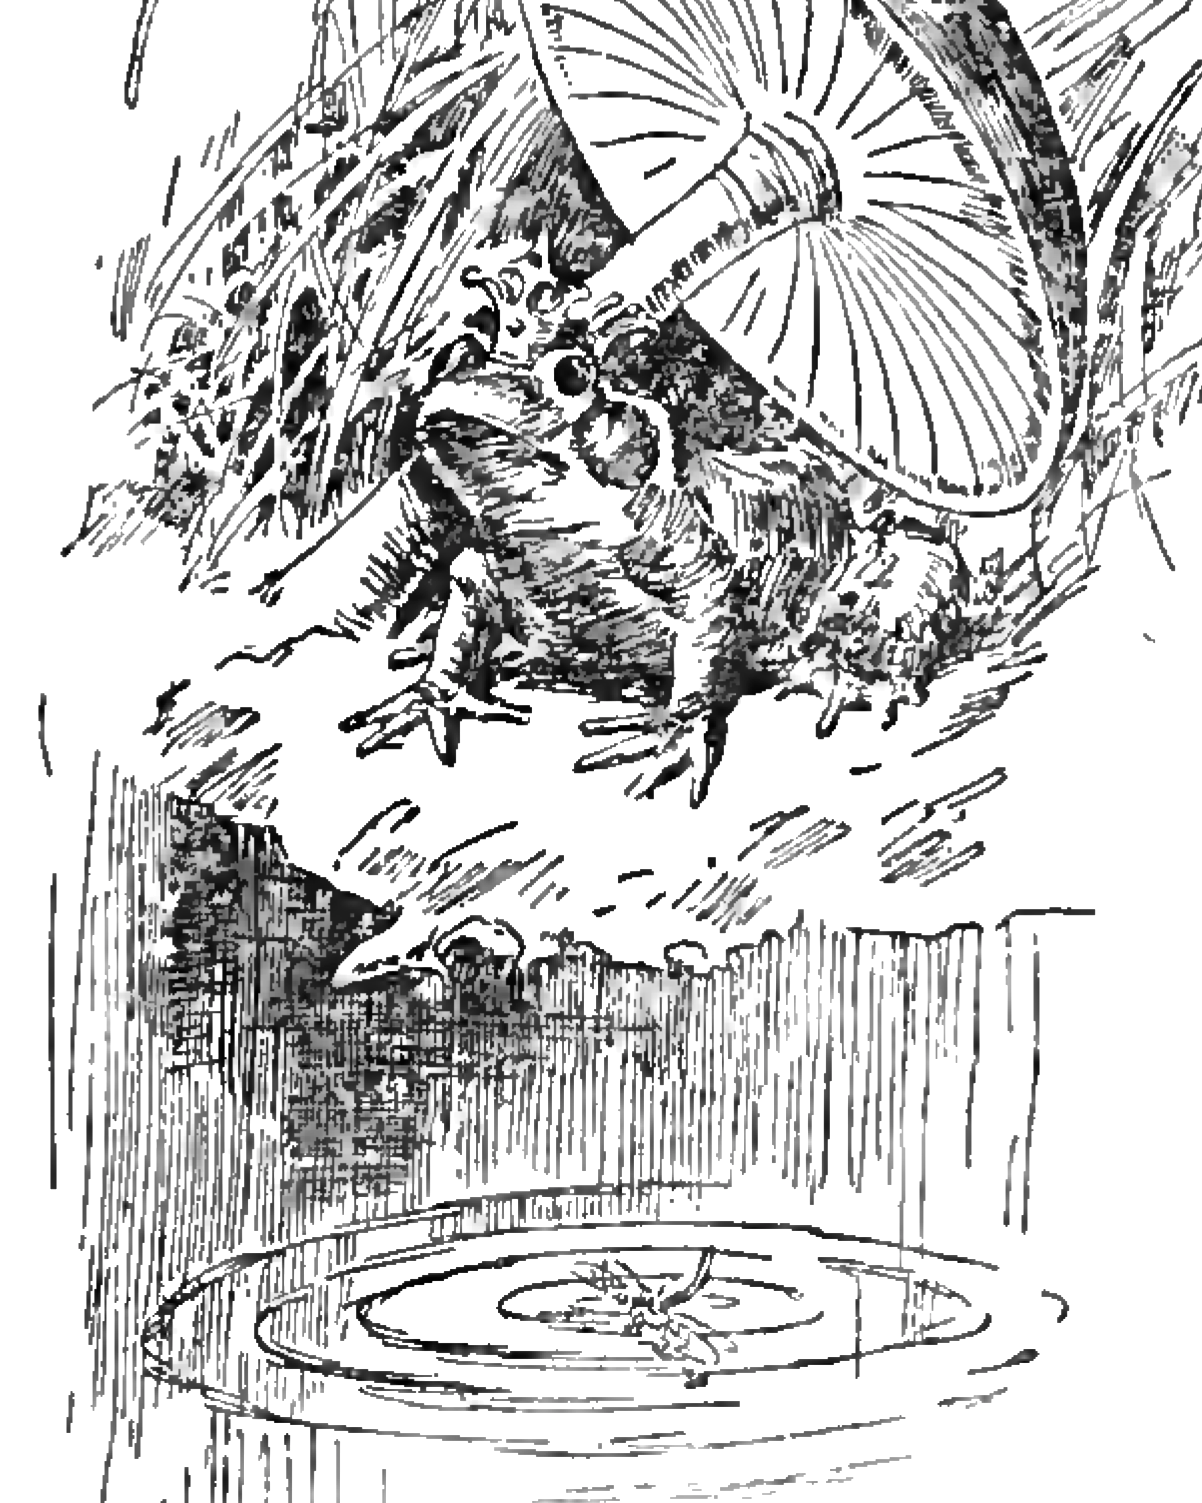
\includegraphics[width=0.78\linewidth]{gfx/frog-prince.png}\footnote{The drawing from \emph{Grimm's Fairy Tales} by \cite{grimmsfairytales1899}}}
	\end{minipage}%
	\caption{Describing the location of target and landmark \textemdash  $\langle$ \textit{frog},\textit{next~to},\textit{pond}$\rangle$.}\label{fig:frog-next-to-pond}
\end{figure}
For example, in `the~frog~next~to~the~pond' the preposition  `next~to' describes the location of the subject `the~frog' with respect to the object `the~pond'. The subject/object are also known by different names, such as \emph{referent}/\emph{relatum} \citep{Miller-JohnsonLaird:1976}, \emph{figure}/\emph{ground} \citep{Talmy:1983} or \emph{located object}/\emph{reference object} \citep{herskovits1986language,Gapp:1994:BasicMeanings,Dobnik:2009dz}.
In this work, we refer to them as  \textsc{Target}/\textsc{Landmark}. 
When referring to a situation with the structure  $\langle\textsc{Target},\textsc{Relation},\textsc{Landmark}\rangle$, 
the expression may be combined with a copulative verb, an existential quantifier or other additional information  (Figure~\ref{fig:frog-next-to-pond}).

In English, there are a small class of words with meanings that denote spatial relations between targets and landmarks. This includes simple words (\emph{on}, \emph{in}, \emph{over}, \emph{under}) and compound phrases (\emph{on top of}, \emph{to the left of}, \emph{to the right of}, \emph{in front of}, and etc.)
Some of these relations are compositional, which means they can be combined to produce new relations (\emph{above} and \emph{far from}). 
Based on the list of prepositions in \citep{landau1993whence}
and alternative compositional and compound relations discussed in  \cite[p.~156]{herskovits1986language}, we created a dictionary of $75$ spatial relations. Considering their alternative forms, with a minor difference in their spatial sense, they constitute $1,194$ entries\footnote{The source code to generate the collection of multi-words expressions is available in the online repository of published studies including \url{https://github.com/GU-CLASP/functional-geometric-lm}.} (Table~\ref{tab:ch2:vocab}). 
For example, `\emph{to the left of}' could be one form of several possible alternative multi-words with close spatial meaning:
\begin{itemize}[topsep=0em,itemsep=0em,partopsep=0em,parsep=0em]
	\item \emph{\{at/on/in/to/by\} the left \{\{hand\} side\} of} $\to$ \emph{to the left of}. 
\end{itemize}

	
\begin{table}[t]
	\begin{tabular}{|lllll|}
		\hline
		about         & above         & across        & after         & afterward     \\
		against       & ago           & along         & alongside     & amid          \\
		among         & apart         & around        & at            & away          \\
		back          & backward      & before        & behind        & below         \\
		beneath       & beside        & between       & bottom        & by            \\
		down          & downstairs    & downward      & during        & east          \\
		from          & front         & here          & in            & inside        \\
		into          & inward        & left          & near          & nearby        \\
		next          & north         & off           & on            & onto          \\
		out           & outside       & outward       & over          & parallel      \\
		perpendicular & right         & side          & sideways      & since         \\
		south         & there         & through       & throughout    & to            \\
		together      & top           & toward        & under         & underneath    \\
		until         & up            & upon          & upstairs      & upward        \\
		via           & west          & with          & within        & without       \\
		\hline
	\end{tabular}
	\vspace{0.5em}
	\caption{The vocabulary of $75$ spatial relations from \cite{landau1993whence} and \cite{herskovits1986language}.}\label{tab:ch2:vocab}
\end{table}


\section{Functional/geometric meaning}
\label{sec:spatial:functional}
Expressing location and describing space is not limited to the prepositional relations in spatial expressions. Other verbs in referring expressions can indicate the relative location between subject and object. With different degrees, these relations might have a strong or weak association with the location of the subject and object. 
For example, `\emph{ride}' entails a specific spatial configuration between the subject and the object, depending on their shape. 
Other relations, such as `\emph{touch}', `\emph{sit on}', and `\emph{jump over}' indicate a specific spatial configuration of subject and object.
Nevertheless, their direct meaning is not just the location of objects; it indicates other kinds of relations, which consequently entail specific spatial arrangements. 

In the same way, the meaning of spatial prepositions is not purely geometrical; it entails other relations and associations between subject and object that are functional. 
The relation  `\emph{over}' does not just describe a geometric location; it also indicates a function \textemdash  the subject provides protection or shelter for the object/s.
The functional sense of relations includes specific interactive relations between entities that are not dependent on the location and spatial configurations.

A simple representation of the geometric sense of relations is based on the acceptability ratings of individual locations with respect to the landmark. 
\cite{logan1996computational} suggest that the mental representation of a geometric meaning could be a template projection of locations on a map, where the landmark is in the middle and each location has its degree of acceptability for the target object. 
A study on location acceptabilities for different prepositions shows that each spatial preposition has a different degree of dependency on object-specific relations  \citep{coventry2001interplay}.
The meaning of each relation is an interplay between the functional and geometric relations of two objects.
For instance, \emph{`above'} has both geometric locational meaning and functional sense. 
When it is used in different context it can have different degree of functional and geometric acceptability.
Spatial relations in natural language have a spectrum of geometricity, with different degree of favouring geometric bias or functional bias. 
Another way to study the object-specific sense of relations is to consider the distributional dependency between relations and objects in image descriptions \citep{Dobnik:2013aa,Dobnik:2014ab}.
In our studies, we consider these aspects of by examining language models.

\section{Image descriptions}
\label{sec:spatial:image}
In a simple \emph{show-and-tell} task, when provided an image, the agent must generate a description of the image. 
Since the early works on human-robot interactions, this task became the centre of interests for natural language grounding \citep{roy2002learning}. 
In recent years, several large datasets have been developed, in which crowd-sourced human annotators describe images from freely available datasets of photographed scenes over the Internet.

\paragraph{Datasets}
Common datasets of image caption tasks, such as MSCOCO  \citep{lin2014microsoft} with more than 300,000 images and Flickr30k  \citep{flickr30k} with 30,000 images, each provide five alternative descriptions per image. 
However, the variation and number of geometric spatial relations in the dataset is limited;
`\emph{to the left of}' and `\emph{to the right of}' are rarely used in the dataset. 
On the other hand, the Visual Genome \citep{krishna2017visual} provides 50 region descriptions and triplet annotations per image, for a total of over 108,000 images. 
The annotation schema, in this case, was slightly different from captioning, as it asks annotators to describe specific parts of the images or the relation between two object areas in the images. 
In this dataset, description and relation annotations are associated with relevant bounding boxes in the image.


\paragraph{Grounding spatial descriptions}
Both generating and understanding a spatial description with three components \textemdash  $\textsc{Target}$, $\textsc{Relation}$, $\textsc{Landmark}$ \textemdash  requires several types of knowledge:
 (1) object identification,
 (2) comprehension of geometric configuration,
 (3) capturing object-specific relations between objects and 
 (4) a frame of reference for projective relations `\emph{to the right of}' and `\emph{below}'.
When people describe image contents, they commonly use spatial expressions. 
A scene can be described correctly using any spatial relation fitting the same objects depending on the intent of the speaker.
However, the image description task may use the knowledge about the scene in a specific way.%
Precisely, object identification and the capture of object-specific relations in the picture might be enough to describe an image with spatial expressions.

\section{Summary}
\label{sec:spatial:summary}
In this chapter, we described the concept of locative expressions and its connection with image descriptions. 
Spatial relations denote locations in scenes. However, their meaning, to some extent, is also dependent on object-specific relations. 
In our studies on grounding spatial descriptions, we will use datasets of images with descriptions, including MSCOCO\citep{lin2014microsoft}, Flickr30k\citep{flickr30k} and Visual Genome \citep{krishna2017visual}.
\chapter{Modelling And Meaning Representation}
\label{sec:concepts}


In this chapter, we address the concepts and the theoretical framework for modelling meaning with uncertainty and grounding natural language in multi-modal representations.

\section{Terminology of modelling}
\label{sec:concepts:model}
Whenever we need to make a systematic prediction based on observations and evidence, we use a set of assumptions. 
A \emph{model} is the encoding of these assumptions in the form of a function. 
This function takes given evidence as input and produces the prediction as an output. Formally, modelling $y$ based on $x$ with the function $f$ would be as follows:

\begin{equation}
y = f_{\Theta}(x)
\end{equation}
\noindent where $f_{\Theta}$ is called the \emph{model function}, which is parametrised with $\Theta$. 

The parameters are part of the assumption about the model function. 
For example, by assuming the rules of physics, the position of a falling object at a specific time in the future can be modelled given the current evident position of the object. 
However, the formula of the location still requires the important parameters of velocity and acceleration of the object in the model. 
More often, determined prediction of an outcome is not enough. We need to associate each prediction with an uncertainty measure. 
Such a model is a \emph{probabilistic model}. 
Instead of modelling the predictable outcome, a measure of uncertainty for any possible outcome is modelled; the density of possible outcomes is conditioned with the observable evidence.
\begin{equation}\label{eq:probabilistic_model}
\mathrm{Pr}( Y=y | X=x ) = f_{\Theta}(y, x)
\end{equation}
\noindent where $f_{\Theta}$ is the model function, which assigns a degree of uncertainty for predicting $y$ grounded on an observable $x$. To simplify the probability annotations, we do not write the complete propositions ($Y=y$); instead, we use shorthand \textemdash  $\mathrm{Pr}( y | x )$.
Commonly, the probability distributions used in this work are categorical, in which $Y$ is a bounded discrete vector of the items. Therefore, the common implementation of function $f_{\Theta}$ is conducted using a module with a vectorised output the same size as $Y$:
\begin{equation}\label{eq:probabilistic_model_module}
f_{\Theta}(y, x) = \mathtt{modules}(x)[y]
\end{equation}
\noindent where $y$ is a category in distribution, the output of $\mathtt{modules}(.)$ is a vector with the size of all possible categories and the square bracket annotation $[y]$ indicates a lookup operation to select the value for $y$-key.

Representing assumptions about the future in a function requires a \emph{framework of modelling} to acquire the model function. 
A constructive \emph{proof}, a search algorithm over a class of functions or its parameters, is the path to building the model function from these assumptions.
When a set of data points drives the search algorithm, the process of fitting a function according to these data points is called \emph{learning} or \emph{training} the model.


\section{Modelling in deep neural networks}
\label{sec:concepts:dl}
In this work, we study the framework of artificial neural networks to encode and build the model function. 
\emph{Deep learning} (DL) and \emph{artificial neural networks} (ANN)
refer to a modelling framework in which a composition of differentiable functions form the model function.
The learning occurs through parameters of the function with the \emph{backpropagation algorithm}.
The backpropagation algorithm is a data-driven optimisation algorithm that uses a measure of error loss over the training data to gradually update the model parameters toward lower error. 
The differentiability of the loss enables this method to apply the chain rule of derivatives to aim the parameter updates toward reducing errors for the training data. 
In a nutshell, the critical assumptions needed to build a deep learning model are the assumed model function (the composition of modules or the neural network architecture), the assumption that the training dataset has relevant knowledge for the task and the assumption about the error function (the loss function).

There are several learning paradigms, such as supervised and unsupervised learning.
These distinctions mainly concern the difference in annotation on the training data, the error function and how they are related to the predictable variable of the model.
The most common paradigm is supervised learning, in which the training dataset is a set of annotated inputs and the predicted output of the model $D = \{(y_i, x_i)\}$.
Unsupervised learning, on the other hand, uses an unlabelled training dataset $D = \{x_i\}$.
The error function in these cases provides additional assumptions about how data points are internally connected. Any internal data structures that indirectly relate to the predictable outcome of the model could be the basis for an error function in unsupervised learning, such as unsupervised clustering of data points for a classification task without supervised data.

The most common loss function for deep learning models is the surprisal of the training data. The surprisal of a random variable ($X=x$) is defined as: 
$\bm{I}_X(x) = -\mathrm{log}(\mathrm{Pr}(X=x))$. 
With a given dataset, such as $D = \{(y_i, x_i)\}$ and a model function $f$, an ideal search algorithm for finds the best fitting parameters that minimise the loss:
\begin{align}
J_\Theta(f,D) &= \sum_{(y_i, x_i) \in D}{-\mathrm{log}(f_{\Theta}(y_i, x_i))} \\
\Theta &= \underset{\Theta}{\mathrm{argmin}} J_\Theta(f,D)
\end{align}
\noindent while the search algorithm looks for the best fitting parameters $\Theta$, there is usually more than one answer or there is no converging path to an acceptable error level with backpropagation. In the most straightforward form \textemdash  backpropagation in a \emph{gradient descent algorithm} \textemdash  the gradient of the error function with a pre-defined learning rate updates all parameters iteratively until the error converges to an acceptable threshold. 
To overcome technical difficulties in processing large datasets and parameter space, other variations of this algorithm may process data in batches, using \emph{stochastic gradient descent} and the momentum of past updates. 
For simplicity, each step of mini-batch training can be formulated as an updating operation for $\Theta$ parameters as follows: 
\begin{equation*}
\Theta = \Theta - \eta \cdot \nabla_\Theta J_\Theta(f; D_{batch})
\end{equation*}
\noindent
where $\eta$ is a hyper-parameter for the learning rate and $\nabla_\Theta$, is a notation for a stochastic deferential operation over every parameter in $\Theta$.

The concept of indirect learning from a function different from the goal prediction of the model is also related to the concept of \emph{multi-task learning} and \emph{transfer learning} in neural networks \citep[Chapter~15]{Goodfellow-et-al-2016}. 
In summary, the parameters of a model function learned from a different dataset or a different goal or a different task encode relevant assumptions needed to make our intended prediction model.
Therefore, the pre-trained modules can be reused or composed into the model function in the neural network. 
The final training steps with much less training data is then known as fine-tuning or in some context referred to as domain adaptation phase.


\section{Grounding in representations}
\label{sec:concepts:grounding}
So far, we have identified that modelling is a way to represent assumptions about the world in the form of the parameters of a predicting function and that DL models encode assumptions inferred from data as a representation space.
The goal of understanding and comprehension is to connect two types of representations \textemdash sensory representations and abstract concepts.
A model that provides the link between two representations is a model of grounded meaning. 
A probabilistic model of representations can potentially formulate such links. 
However, the question remains about the generalisability of the learning (see section~\ref{sec:concepts:compositionality}).

By definition, the model represents the uncertainty of connecting observables to their representation; therefore, it can be used as a model of \emph{grounded representations}. 
Within the paradigms of DL, instead of having a given strict symbolic representation for concepts and their internal associations, these representations must be learned. 
The architectural design of the neural networks and the training datasets impose restrictions on how these representations are interconnected. 
In the machine learning community, this has become a field of study called \emph{representation learning} \citep{bengio2013representation}. 

When modelling conversational agents, linguistic expressions are grounded in internal representations of the agent. There are at least two probabilistic models of meaning for (1) generating and (2) understanding utterances:
\begin{align}
\mathrm{Speaker~model}:& \mathrm{Pr}(u | r) = f_{\Theta_s}(u, r) \label{ch3:eq:utt}\\
\mathrm{Listener~model}:& \mathrm{Pr}(r | u) = f_{\Theta_l}(u, r)
\end{align}
\noindent $\mathrm{Pr}(u | r)$ is the measure of uncertainty in choosing the utterance  $u$, referring to the given representation  $r$. 
$\mathrm{Pr}(r | u)$ is the measure of uncertainty in interpreting the given utterance $u$ as if it meant representation $r$ for the listener. 
In other words, the grounded meaning of each natural language utterance is what it denotes in the representation space according to the model.
Without any probabilistic sampling in composition of modules in neural networks, there is unambiguous mapping of sensory representations onto grounded representation space. 
However, the link between grounded representations and natural language utterances is uncertain, with a linking degree of uncertainty on all possible outcomes. 
The learning process establishes the degree of certainty of the link between utterances and representation space and builds the fitting map between the agent’s primitive sensory and motor representations and grounded representation space. 

Later, in section~\ref{sec:concepts:glm}, we provide additional discussion about the link between meaning and representations in the speaker model. 
In a speaker model, to express what is in an image, the sensory data for the situation is first mapped onto the representation space ($\raisebox{-0.3\height}{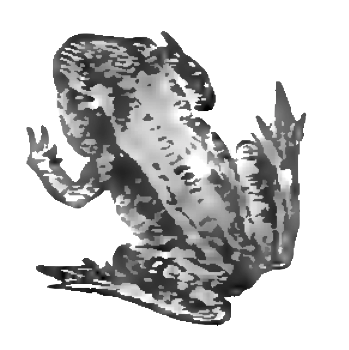
\includegraphics[width=0.5cm]{gfx/frog.png}} \Rightarrow v$). Then, the speaker model assigns a measure of goodness to the utterance predictions:
\begin{equation*}
\mathrm{Pr}(\mathrm{``there~is~a~frog"} | v) = f_{\Theta_s}([\mathrm{``there"},\mathrm{``is"},\mathrm{``a"},\mathrm{``frog"}], v)
\end{equation*}
\noindent In other words, the model of grounded meaning is also a model for connecting utterances to sensory evidence. 
The internal representations are not directly connected to external references. 
They are interpretations of the sensory readings internal to the agent. 
The mapping function between visual sensory inputs and internal agent representations could be modelled with a pre-trained convolutional network enriched with other contextual information about the situation. %
The model establishes uncertain links between primitive sensory readings and utterances of natural language, for that reason it functions as a model of grounding. 
In section~\ref{sec:concepts:convnets}, we describe some properties of this representation space and how sensory features would be mapped onto this representation space.




\section{Modelling compositionality}
\label{sec:concepts:compositionality}
One of the challenges of a model of grounding is formulated as Harnad’s symbol grounding problem \citep{harnad1990symbol}. 
The argument is that the capacity of learning from limited data is problematic when it is expected to impose new links to potentially unlimited compositions in a symbolic representation system.
The challenge is to infer grounded meanings for new representations (e.g. \textsc{`zebra'}) from known bottom-up representations learned from images (e.g. \textsc{`horse'} and \textsc{`stripes'}) 
when a symbolic link between them (\textsc{`zebra'} and a composition of two others) is established in natural language (\textsc{`zebra'} = \textsc{`horse'} + \textsc{`stripes'}).
In other words, compositionality as an ability to construct new representations linked to both sensory and abstract linguistic representations creates a generalisation problem for bottom-up learning.
The underlying premise of Harnad’s formulation of the problem is that human language is symbolic;
therefore, when human behaviour shows the capability of learning from language input, the establishment of such links came from new symbolic rules imposed by new statements of the natural language.

Without this explicit premise about the nature of language, the recent literature of language modelling stretches the notion of compositionality. 
In one account, any function in a semantic vector space is a model of compositionality \citep{mitchell2010composition}. 
In another direction, the semantic parse trees of linguistic expressions are used for composing neural network modules \citep{andreas2016neural}.

The notion of compositionality in natural language that we use in this thesis is simply the extent of generalisation in bottom-up training. 
The grounding of known representations is the learned link between natural language utterances and their internal neural representations.
The representation space imposes the compositional and structural links (\textsc{`zebra'} = \textsc{`horse'} + \textsc{`stripes'}), which are either learnable without intrinsic structures in space from data or learnable with extended structural or top-down control or design of the intrinsic properties’ representation units.



\section{Generative language model}
\label{sec:concepts:glm}
When the target of predictions in Equation~\ref{eq:probabilistic_model} is a linguistic unit, the model is what we call a \emph{probabilistic language model} \textemdash predicting the next word given previous sequences of words.
\begin{equation}\label{ch3:eq:lm0}
\mathrm{Pr}( w_{t+1} | w_{1:t} ) = f_{\Theta}(w_{t+1}, w_{1:t})
\end{equation}
\noindent where $w_{1:t}$ represents the given sequence of words at time step $t$ and the random variable is the target token at time $t+1$, here represented with a shorthand annotation for the probability of $w_{t+1}$. The sampling process from this model can potentially be part of a model designed to generate sequences of any length:
\begin{equation}\label{ch3:eq:lm}
\mathrm{Pr}( w_{1:T} ) = \prod_{t=1}^{T-1} \mathrm{Pr}( w_{t+1} | w_{1:t} )
\end{equation}
\noindent when coupled with a search algorithm, such as beam search, can be used for language generation. When the model function is based on recurrent neural networks, we call it a \emph{recurrent generative language model}, shortened to a \emph{recurrent language model}:
\begin{align}
\mathrm{Pr}( w_{t+1} | w_{1:t} ) &= f_{\Theta}(w_{t+1}, h_t) \\
h_t &= \mathtt{rnn}_{\theta_1}(h_{t-1}, w_t) \\
f_{\Theta}(w_{t+1}, h_t) &= \mathtt{softmax}(g_{\theta_2}(h_t))[w_{t+1}]
\end{align}
\noindent where $h_t$ represents the recurrent state at time $t$. 
This could also be interpreted as an agent representation in Equation~\ref{ch3:eq:utt} for generating each token. 
Two important modules of the language model are  $\mathtt{rnn}_{\theta_1}$, the recurrent module, and $g$, the top module, often a multi-layer perceptron, the output of which is a vector with the size of the vocabulary. In the end, $\mathtt{softmax}$ is the final activation function over all possible tokens in the vocabulary:
\begin{equation}
\mathtt{softmax}(V) = [\frac{e^{x}}{\sum\limits_{x' \in V}{e^{x'}}}]_{x \in V}
\end{equation}
\noindent where $V$ represents a vector of vocabulary size. After activation with $\mathtt{softmax}$, the output resembles a categorical probability distribution of the vocabulary.
The notation $\mathtt{softmax}(\cdot)[w]$ represents the predicted probability for $w$ at the output vector.
The unfolded representation of the model function would be as follows:
\begin{equation*}
\mathrm{Pr}( w_{t+1} | w_{1:t} ) = f_{\Theta}(w_{t+1}, \mathtt{rnn}_{\theta_1}(\mathtt{rnn}_{\theta_1}(...\mathtt{rnn}_{\theta_1}(h_0,w_{1})..., w_{t-1}), w_t))
\end{equation*}
The parameter set of the model, $\Theta$, is comprised of two partitions, ${\theta_1, \theta_2}$, from the two main modules of the model. 
The most common recurrent neural network we will use in this thesis is long-short term memory (LSTM) \citep{hochreiter1997long}.
We often add a trainable embedding layer in addition to the recurrent neural network to learn token representations. 
When a generated utterance is supposed to describe the content of an image or other situation, the generative language model in Equation~\ref{ch3:eq:lm0} and \ref{ch3:eq:lm} could be written as a conditional probability similar to the speaker model in Equation~\ref{ch3:eq:utt}: 
\begin{align}
\mathrm{Pr}( w_{t+1} | w_{1:t}, c ) &= f_{\Theta}(w_{t+1}, h_t, c) \label{ch3:eq:token_model}\\
\mathrm{Pr}( w_{1:T} | c)           &= \prod_{t=1}^{T-1} \mathrm{Pr}( w_{t+1} | w_{1:t}, c )
\end{align}
\noindent where $c$ represents the encoding of the situation \textemdash  visual features and the fusion of two representations, $h_t$. $c$ is the agent’s grounded representation in the speaker model in  Equation~\ref{ch3:eq:utt}. 

In these models, the uncertainty measures of the language model could also be interpreted as the degree of acceptability of linguistic units. 
With the speaker rationality assumption, the distribution of utterances in training data should not be very different from the acceptability judgment rankings. 
The generative language model learned from this data is also a model of acceptability judgments. If the language model can accurately predict acceptability judgments, it can be considered a model of syntax. 
It has been argued that such a language model is also an implementation of syntax without underlying categorical syntactic rules \citep[Section~3]{lau2017grammaticality}.

On the other hand, predicting the categorical distribution of tokens in their positions is, in fact, a model for the substitutability of words (i.e. Equation~\ref{ch3:eq:token_model}). 
Such a model loosely simulates substitutability of tokens.
Therefore, the vector representations learned for tokens and words in these models loosely posses the attributes for lexical-semantic representations.
This notion of meaning representation is consistent with the grounded representation discussed in section~\ref{sec:concepts:grounding}.
Based on these two arguments, a neural language model must be able to encode knowledge about syntax and semantics in the form of the neural network modules’ structure and parameterised representations. 
To predict the model outputs, parameters such as embeddings and intermediate representations of modules (contextualised embeddings) encode relevant knowledge learned from the training data.


\section{Modelling convolutional neural networks}\label{sec:concepts:convnets}
In section~\ref{sec:concepts:grounding}, we mentioned the possibility of using a function such as convolutional networks to map visual inputs onto a representation space for language grounding.
Here we discuss two aspects of using convolutional neural networks as a feature extraction function:
\begin{itemize}
	\item[(1)] How do convolutional neural networks process images?%
	\item[(2)] What types of knowledge are encoded in convolutional representations?
\end{itemize}

The role of convolutional networks (ConvNets) as a mapping function is to take basic two-dimensional pixel representation of images from a colour feature space, then project it onto another feature space that can discriminate images based on their content.
The most basic form of visual understanding is to recognise objects and entities in images.
A set of features that can distinguish visual differences between objects would be enough for most tasks.
For this reason, the most common way to use ConvNets in a variety of visual processing tasks is to train it as a module in an object recognition model, then use it as feature extraction module in other tasks and models.
The success of ConvNets in an object recognition task \citep{krizhevsky2012imagenet} with a large ImageNet dataset  \citep{deng2009imagenet} was the landmark deep learning success in computer vision. 

Conceptually, an object recognition model has the following modular design:
\begin{align}
\mathrm{Pr}( category | I ) &= f_\Theta(category,I) \\
\mathbb{V}_{I}              &= \mathtt{ConvNet}_{\theta_1}(I) \\
f_\Theta(category,I)        &= \mathtt{softmax}(\mathtt{mlp}_{\theta_2}(\mathtt{flatten}(\mathbb{V}_{I})))[category]
\end{align}
\noindent where $f$ is the uncertainty model for recognising a category of the object given the image $I$. 
The model has two modules \textemdash $\mathtt{ConvNet}_{\theta_1}$, the convolutional network for feature extraction and $\mathtt{mlp}_{\theta_2}$, the multi-layer perceptron for classification based on convoluted features. The most important property of ConvNets is that it can transfer object recognition knowledge to find patterns of local structures \citep{lecun2010convolutional}.

For recognising objects, we need a feature representation that would be, to some extent, invariant to spatial transformations. Geometric transformations such as shifting, rotating and rescaling have limited effects on recognising an object. Notable image representations such as the scale-invariant feature transform (SIFT) \citep{lowe2004distinctive} and the histogram of oriented gradients (HOG) \citep{dalal2005histograms} were motivated by this requirement. 
However, object recognition is not strictly invariant to geometric transformations. Spatial compositions at a global level can change the interpretation of smaller patterns. 
For these reasons, ConvNets was designed with the prior knowledge that identifying local patterns in different scales is essential. 
Then, for all possible regions of the image, as pre-defined granularities, their receptive fields would be mapped onto a new feature space. 
The feature mapper (or the kernel function)
with input as small as 3x3 pixels interprets local regions into a new representation space.
The term \emph{convolutional network} refers to multiple stages of feature mapping followed by spatial sub-sampling, which finally produces a representation with a coarser space but richer representations. 
After stacking the modules of feature mapping with sub-sampling, each broader region is mapped to a vector representation.

Although prior knowledge about the task led to its design and the popularity of ConvNets in several tasks, there is limited theoretical understanding about how and what geometric features are encoded in convoluted representations.
Based on one account, these features are useful for localisation and object detection tasks, without an algorithmic search \citep{Lenc15a,ren2015faster}. 
In another account, the recognition tasks are sensitive to local geometric transformations\footnote{The recognition of a face depends on the spatial relationships between eyes and nose \citep{hinton2011transforming}}
and ConvNets relax the geometric knowledge; therefore, geometric relationships between local parts in lower layers decay when reaching the higher layers \citep{hinton2011transforming,lenc2015understanding,kelleher2017what}. 

Based on these two accounts:
\begin{itemize}
	\item[(1)] The geometric features in convolutional representations are a continuum of relational features among smaller regions and larger super-pixels;
	\item[(2)] These are locally relaxed at the final layers to the extent that convolutional representation may have lost its geometric knowledge.
	This is an important consideration when we want to ground spatial relations in natural language on these visual representations.
\end{itemize}

\section{Conclusion}
\label{sec:concepts:conclusion}

We explained that any modelling requires a set of assumptions; modelling with neural networks encodes these assumptions into the model architecture, training datasets and objectives. 
We addressed the neural network modelling for grounded representations, compositionality and language generation. 
All these models correspond to challenges in meaning representations. 
In the next chapter, we summarise our studies on spatial knowledge encoded in the language models.
\chapter{Summary Of Studies}
\label{sec:related}



In this chapter, we summarise the questions, methods and findings of six studies and discuss their relevance to the main aims of the thesis.

\section{Study 1: Functional/geometric bias in neural language models}
\label{study:fungeo}
Simon Dobnik, Mehdi Ghanimifard, and John Kelleher. 
Exploring the Functional and Geometric Bias of Spatial Relations Using Neural Language Models.
\textit{In Proceedings of the First International Workshop on Spatial Language Understanding, pp. 1-11. 2018.}

Understanding spatial language is fundamental to human-robot interactions. 
The meaning of spatial relations in scene descriptions is grounded in the geometry of the scene and the functional relationship between objects. 
We used a neural language model on a large corpus of image descriptions to investigate the earlier observations about functional bias in spatial relationships.
We contributed to understanding that are encoded in unimodal neural language models.

\subsection{Questions}

Does the performance of trained neural language models on relational descriptions in the Visual Genome dataset  \citep{krishna2017visual} account for the expectation that more functional spatial relations are more predictable based on the objects they describe? 

We propose two hypotheses: 
\begin{itemize}
	\item Descriptions with functional relations (in contrast with geometric relationships) have lower perplexity in their language model over the held-out test suite (more likely gold-standard descriptions) because they describe a functionally common situation. The target/landmark object pairs in the dataset are more specific to functional relations compared to geometric relations. 
	\item When modifying spatial relations with any alternatives, the phrases with the initial choice of functional relations gain increased perplexity because they are more contextually dependent on targets and landmarks compared to geometric relations.
\end{itemize}


\subsection{Method}
We trained the neural language model on image descriptions in Visual Genome. Then, we measured the perplexity of the model on held-out descriptions based on their spatial relations. In our experiments, we examined the hypothesis on both natural occurring descriptions in the dataset and the down-sampled balanced dataset.

\subsection{Findings and conclusions}
We observed from the perplexity of the language model that functionally-biased spatial relationships are more predictable when the model was trained on the dataset with a naturally occurring frequency of descriptions.
However, training the model on a down-sampled dataset did not result in the expected outcome of perplexities for each test group.%
We reported a more detailed examination of sensitivity %
of the language model.
Our observation showed that the degree of sensitivity for target and landmark is not the same in the two groups of spatial relations. 
A possible explanation for different sensitivity for targets and landmarks is the misalignment between word order, semantic structure of relations and the cognitive process of choosing related objects as landmark and target. 
Misalignment of word order and the underlying semantic structure of spatial expressions explains why the forward and backward direction language models have different levels of perplexity.

The second category of the hypothesis was only partially confirmed. 
Only a few spatial relations confirmed the hypothesis. 
While some geometric relations, such as \emph{`above'} tend to see a high degree of change in perplexity when replaced with other spatial relations, the dependency of geometric relations on the textual context leaves interesting open questions about the world knowledge and spatial knowledge in neural language models.

\paragraph{Author contributions}
Mehdi Ghanimifard had the main responsibility for implementing the model, conducting the experiments and reporting it. Simon Dobnik and John Kelleher had shared responsibility for the remaining aspects of this research. All authors read and approved the final manuscript.

\section{Study 2: Representation of spatial relations in neural language models}
\label{study:what}
Mehdi Ghanimifard and Simon Dobnik. 
\emph{What} a neural language model tells us about spatial relations.
\textit{In Proceedings of the Combined Workshop on Spatial Language Understanding (SpLU) and Grounded Communication for Robotics (RoboNLP), pp. 71-81. 2019.}

We followed up the question about possible encoded knowledge in section~\ref{study:fungeo} about spatial relations in unimodal neural language models.
In this work, we extend the method to inspect the knowledge of spatial relations in generative language models. 
One of the methods for measuring lexical knowledge in distributional semantics is analogical reasoning tasks. 
The knowledge of spatial relations in the image description task may be different from the visual-cognitive knowledge required for human judgment on spatial relations, so we also examined if learned representations are transferable to other tasks.


\subsection{Questions}
\begin{itemize}
	\item What should we expect from a contextualised model of spatial relations based on textual features in terms of their functional and geometric bias?
	\item How can we inspect these in a generative language model? 
	\item How do the learned representations from the generative model compare with representations from human judgments?
\end{itemize}

\subsection{Method}

We trained a generative LSTM language model on region descriptions. 
Then, we inspected %
how the language model encodes descriptions of spatial relations in swapped contexts of target and landmark objects in terms of perplexity.
We proposed a method in which word-context vectors are produced based on augmented datasets, swapping spatial relations in the context of other spatial relations. Perplexities of these generated word-context examples built perplexity-based vector space for spatial relations. 

We ran analogical tests on these vectors and other textual embeddings to inspect how these representations differed from each other. 
Finally, we compared them with vector representations of human acceptability judgments and relatedness judgments.

\subsection{Findings and Conclusions}
In the absence of the image, we expected contextual representations to learn object-specific knowledge (functional knowledge). 
However, the learned representations showed high performance in solving analogical tasks that required also some sense of geometry. 
Our analysis is that functional knowledge must be complementary to geometric knowledge, which is why language models can partly solve these puzzles. 
These finding were also confirmed with qualitative inspections,
for example
the representations of \emph{`left'} and \emph{`right'} were similar to each other and different from \emph{`above'} and \emph{`over'}.

The task of judging acceptabilities, the task of generating descriptions and annotations, and the task of finding related words are three different tasks, perhaps using different kinds of spatial knowledge.
The last experiment comparing the similarities of representations in the image description task, acceptability judgments and relatedness experiments hinted that spatial relations in the image description task might use different types of knowledge about space and spatial relations. 

The findings of this study raise questions that links this study to study four and five.
Knowing that textual context provides discriminative features for identifying spatial relations, we argue that, in language generation tasks, one can ground the word choices in textual evidence. 
Generative neural language models can encode task-specific knowledge of space, including functional and geometric bias, when describing the relation between two objects. 
With this insight, the consequence of memorised knowledge is an open question for multimodal language models \textemdash how does a multimodal language model balance the attention to knowledge of the scene and linguistic representations in the task? 

\paragraph{Author contributions}
Mehdi Ghanimifard had the main responsibility for implementing the model, conducting the experiments and reporting it. Mehdi Ghanimifard and Simon Dobnik had shared responsibility for the remaining aspects of this research. Both authors read and approved the final manuscript.

\section{Study 3: Functional/geometric spectrum in bounding boxes}
\label{study:bbox_grounding}
Simon Dobnik and Mehdi Ghanimifard. 
Spatial descriptions on a functional-geometric spectrum: the location of objects.
\textit{Preprint - 2020.}

In the previous two studies, we investigated the distributional properties of spatial relations in language. 
We argued that functional knowledge and geometric knowledge are encoded in distributional representation, which can be captured to some extent with neural language models. 
To complement this study on the grounding of spatial relations for image descriptions, we extended the investigation on the distributional properties of bounding boxes for the spatial relations that describe them. 
More specifically, in this study, we used bounding boxes to extract the basic geometric features of the relations between two objects. 
Then, we inspected the geometric feature distribution of each %
spatial relation.

\subsection{Questions}
\begin{itemize}
	\item Are the bounding box features extracted from annotated images reliable descriptors for spatial relations; do the extracted features correspond to other geometric representations, such as spatial templates? 
	\item Are geometrically biased spatial relations%
	obtained in constrained experimental settings
	reflected in more predictable locations of objects?
	Can they be mapped into fewer variations of their related object locations?
\end{itemize}

\subsection{Methods}
For each relation, we collected the pairs of bounding boxes from the relationship dataset in the Visual Genome \citep{krishna2017visual}. 
After standardising the bounding boxes, each pair of objects produced several feature vectors $[x, y, d]$.  Inspired by the Attentional Vector Sum (AVS) model  \cite{RegierCarlson:2001},
the bounded boxes were converted to feature vectors that expressed the geometric relations between individual locations of objects.
The expected feature vectors for each spatial relation 
are
comparable with %
spatial templates. 
Then, we inspected the variations and skewness of the feature vector distributions from their centroid to determine if this%
accounts for geometric bias.  
The lower the variation, the more geometrically biased is the relation.

\subsection{Findings and conclusion}
We found that the bounding box features %
represented as the
weighted sum vectors from acceptability scores in spatial templates for projective relations. 
We found that the feature vectors for geometrically biased relations diverge less from the average vectors compared to their more functionally biased equivalent relations. 
The distribution of feature vector divergence from the average vector is more skewed toward zero when they describe a geometrical relation. 
We also inspected the properties of some verbal relations with spatial content. 
These spatial features indicate spatial regularities in the image description dataset.
Practically, the findings of this study would be helpful when designing models for image captioning, as it demonstrates the representations that are relevant for different types of descriptions.

\paragraph{Author contributions}
Mehdi Ghanimifard had the main responsibility for implementing the model, conducting the experiments and reporting it. Simon Dobnik and Mehdi Ghanimifard had shared responsibility for the remaining aspects of this research. Both authors read and approved the final manuscript.

\section{Study 4: Evaluating generation of spatial descriptions with adaptive attention}
\label{study:knowing}
Mehdi Ghanimifard and Simon Dobnik. 
Knowing When to Look for What and Where: Evaluating Generation of Spatial Descriptions with Adaptive Attention.
\textit{The European Conference on Computer Vision (ECCV) Workshops, pp. 153-161. Springer, Cham, 2018.}

The neural network model in \citep{lu2017knowing} provides an attention mechanism that expands the domain of attention from spatial attention on visual features to hidden states in the language model. 
In sections~\ref{study:fungeo}~and~\ref{study:what} we explored the possibility of memorising specific spatial knowledge in a unimodal language model, including functional and task-specific spatial relations between objects. 
In this study, we wanted to determine how a multimodal language model uses it in a language generation task. 
The attention on linguistic features when knowledge from different sources generating different parts of speech and,
more specifically, on spatial relations can explain the grounding of the generation model in multimodal information, including the contextual representations in the language model memory. 

\subsection{Questions}
\begin{itemize}
	\item How does the attention on visual features and linguistic features change for different parts of speech?
	\item Is there any difference in the magnitude of attention on visual features between targets and in landmarks?
	\item Are spatial relations grounded in visual features? %
\end{itemize}

\subsection{Method}
The adaptive attention between visual features and linguistic features compete with each other. 
The magnitude of attention on linguistic features is a sign of dependence on language and context instead of a grounding in visual features.
In this study, we inspected adaptive attention as a source of explanation for grounding. 
The average of attention on linguistic features for each part of speech and, for each semantic role in spatial descriptions (target, relation, landmark) is interpreted as an indication for a lack of visual grounding.
We compared the 
ranking
of attentions with the rankings of accuracy rates of a uni-modal language model predicting a mismatch, whether a part of speech has been replaced in the FOIL captions \citep{shekhar2017vision}. %
We also qualitatively examine the average spatial attentions of descriptions containing each spatial relation; the spatial attention on target, landmark and spatial relation.

\subsection{Findings and conclusion}

The degree of attention on linguistic features varies depending on the part of speech. In particular, we found that the attention on visual features drops when predicting spatial relations compared to the average attention on noun phrases. 
The average visual attention on parts of speech partially reflected the results from the FOIL task. For example, nouns are highly visually attended but difficult to predict by the language model, the adpositions (prepositions and postpositions) were ranked among the least visually attended parts of speeach while there were moderately predicatable in the FOIL task.

There are three possible explanations for these results:%

\begin{itemize}
	\item[(1)] Spatial relations are more functional and object dependent in these tasks. Therefore, object-specific spatial features (spatial affordances of objects) encoded in language models are more likely to be predictive of spatial relations than visual clues in the image.
	\item[(2)] CNNs do not have 
	represent geometric
	locational information required for grounding spatial relations. As they are trained for object identification, there is some degree of spatial invariance in these features.
	\item[(3)] Using softmax for modelling attention is a 
	disadvantage 
	in cases where spatial attention is distributed over several objects and their relation.
	Spatial relations depend on target, landmark and locational features; therefore, the softmax model of attention is noisier when it attends to multiple locations for predicting spatial relations.
\end{itemize}


\paragraph{Author contributions}
Mehdi Ghanimifard had the main responsibility for implementing the model, conducting the experiments and reporting it. Mehdi Ghanimifard and Simon Dobnik had shared responsibility for the remaining aspects of this research. Both authors read and approved the final manuscript.

\section{Study 5: Generating descriptions with top-down spatial knowledge}
Mehdi Ghanimifard, and Simon Dobnik. 
What Goes Into A Word: Generating Image Descriptions With Top-Down Spatial Knowledge.
\textit{In Proceedings of the 12th International Conference on Natural Language Generation. 2019.}


As we continued to question how the neural language model learns spatial knowledge, we investigated the effects of top-down knowledge on space in generating relational image descriptions. As seen in section~\ref{study:knowing}, the attention mechanism for the generative recurrent language model can control and explain how different modalities contribute to generation tasks. In this study, we integrated 
specific geometric and non-geometric features that are considered relevant in top-down computational models
of spatial descriptions into the design of the attention model. We compared the effects of three types of top-down spatial knowledge: 
\begin{itemize}
	\item[(1)] Where objects are obtained with a separate localisation procedure;
	\item[(2)] Which object is the target, and which is the landmark, with prior role assignment;
	\item[(3)] How they are geometrically related in images by representing their spatial configuration.
\end{itemize} 

\subsection{Questions}
\begin{itemize}
	\item[(1)] Which types of top-down spatial knowledge improve language generation? 
	\item[(2)] How does each category of features contribute to generating image descriptions?
\end{itemize}

\subsection{Method}
We experimented on a relationships dataset from the Visual Genome  \cite{krishna2017visual}, training several comparable neural network designs with different spatial modules 
and different types of top-down knowledge about spatial relations. 
We changed the attention module in these models 
to be able to attend over language model features, visual features and geometric features
and enriched the %
input representations with 
the additional geometric features representing the spatial configurations of objects.
In addition to comparing the performance loss on unseen examples, we inspected the attention module to determine what features had a dominant effect on generating descriptions.

\subsection{Findings and conclusions}
We observed that the overall performance improved with the additional top-down knowledge of space. 
However, the results showed a substantial contribution of the %
language model representations in generating descriptions. 
Among added spatial knowledge localisation had the strongest effect, while the effects of role assignment and geometric spatial features were mixed. 
The reasons behind this outcome may be the bias in two kinds of regularities in data \textemdash the spatial composition of objects in photos in this dataset (location of objects are meaningful from the perspective of the photographer) and the task of describing object relations may have neglected the application of certain geometric relations (\emph{`to the left of'}, \emph{`to the right of'})
but preferring general, less specific spatial relations such as \emph{`close'} and \emph{`with'}.

\paragraph{Author contributions}
Mehdi Ghanimifard had the main responsibility for implementing the model, conducting the experiments and reporting it. Mehdi Ghanimifard and Simon Dobnik had shared responsibility for the remaining aspects of this research. Both authors read and approved the final manuscript.

\section{Study 6: Learning to compose grounded spatial relations}
Mehdi Ghanimifard and Simon Dobnik. 
Learning to Compose Spatial Relations with Grounded Neural Language Models.
\textit{In IWCS 2017-12th International Conference on Computational Semantics-Long papers. 2017.}


A basic definition of grounding linguistic units in visual perception is to associate words and phrases with visual features. 
Learning these associations must generalise from limited examples to 
novel
unseen compositions.
Compositionality in language imposes a systematic generalisation to the grounding of words and phrases. 
Due to the broad application of recurrent neural language models in vision and language tasks, this study investigated the capability of a recurrent language model in learning these compositional generalisations in the grounded language.

\subsection{Questions}

\begin{itemize}
	\item To what extent is the language model trained on single examples can retrieve acceptability representations about the scene? 
	\item Is the recurrent language model capable of generalising from word compositions to phrase compositions and how does it perform over previously unseen word compositions?
\end{itemize}

\subsection{Method}
Simple spatial relations are composable and can be used to construct new relations, such as \emph{`above and to the right of'}, which denotes a relation constructed from two simple relations \emph{`above'} and \emph{`to the right of'}. We constructed artificially composed spatial templates based on their acceptability scores
of the individual
the spatial templates \citep{logan1996computational} using known compositional operations. 
Then, from these templates we generated synthetic 
examples of individual situations and descriptions based on the aggregated acceptability scores.
We tested different learning scenarios by controlling for unseen descriptions. 
In each experiment, we reconstructed the spatial templates of unseen descriptions based on the model scores over
the unfolded predictions of words.
Qualitatively, we measured the mismatches between the reconstructed templates and 
templates that were used to generate the artificial training data.

\subsection{Findings and conclusions}
We found that a grounded neural recurrent language model is capable of generalising when composing and decomposing word sequences both across the language and the perceptual domain.. 
We investigated the effects of three factors on the success of the task and found that the degree to which the training data was impoverished had the most substantial effect, the type of composition is an essential factor in learning compositionality, and the presence of ungrounded distractor words had a small effect.

These observations leave an open question \textemdash is the performance for certain compositions reliant on intrinsic structures of recurrent neural networks for learning specific functions or the frequency and variation of data due to the semantic and combinatorial properties of compositions? 
Negation has fewer possible variations compared to \textsc{`or'} phrases and \textsc{`and'} phrases; 
therefore, it produces fewer instances and fewer variations in the training data for the negation marker. 
Distribution of the training data affects the final learned embeddings for the tokens of \textsc{`and'}, \textsc{`or'} and \textsc{`not'}. 
Learning to encode negation as a function in the recurrent unit might be harder than encoding other functions. 

In summary, the combinatorial properties and semantics of different compositions affect the frequency and distribution of all tokens in language. 
While the distributional effects have potentially challenging consequences for the uniform learning of compositions, it can signal the difference between them.
This is why, despite the imbalance in the number of compositions, the model could learn not ground distractor tokens.%

\paragraph{Author contributions}
Mehdi Ghanimifard had the main responsibility for implementing the model, conducting the experiments and reporting it. Mehdi Ghanimifard and Simon Dobnik had shared responsibility for the remaining aspects of this research. Both authors read and approved the final manuscript.

\section{Study 7: Metaphoricity of compositions with distributional representations}
Yuri Bizzoni, Stergios Chatzikyriakidis and Mehdi Ghanimifard. 
``Deep'' Learning: Detecting Metaphoricity in Adjective-Noun Pairs.
\textit{In Proceedings of the Workshop on Stylistic Variation, pp. 43-52. 2017.}

Recognising metaphoric use of language requires an understanding of the situation, context and how expressions refer to extra-linguistic knowledge about the world. 
On the other hand, distributional knowledge in unimodal language models encodes word-context associations. 
Even without the presence of extra-linguistic knowledge of situations, distributional knowledge might be able to determine metaphorical adjective-nouns. 
In this study, we proposed that knowledge of the compositionality of adjective-nouns is encoded in the pre-trained word embeddings of textual corpora and a simple neural network can transfer this knowledge to metaphor recognition tasks. 
We used methods of vector composition in a neural network design to predict the metaphoricity of adjective-noun compositions.


\subsection{Questions}

\begin{itemize}
	\item Is it possible to detect metaphoric adjective-noun compositions using pre-trained word embeddings in a shallow neural network? 
	\item Are there any differences in performance between design choices and language model types, including word2vec \citep{mikolov2013distributed}, GloVe \citep{pennington-etal-2014-glove}, and dependency-based embeddings \citep{levy-goldberg-2014-dependency}?
\end{itemize}

\subsection{Method}
We compared different methods of vector composition in a neural network design, similar to \cite{mitchell2010composition}, and used different pre-trained word embeddings. 
We examined the performance of these models with cross-validation on unseen adjectives and unseen adjective-noun pairs.

\subsection{Findings and Conclusions}
We found that pre-trained word embeddings with simple neural network designs performed better than previous approaches without using word embeddings. 
This study raises a question if similar designs could expand metaphoricity judgments to other part-of-speech compositions. 
The high performance of the textual word embeddings up to 93\% accuracy confirms that unimodal language models can encode some knowledge of the referential meaning to real situations. 
However, questions concerning the type of knowledge and it are left for subsequent studies.

\paragraph{Author contributions}
Mehdi Ghanimifard had the main responsibility for writing the model section of the manuscript. Mehdi Ghanimifard and Yuri Bizzoni had shared responsibility on running the experiments and reporting it. Yuri Bizzoni and Stergios Chatzikyriakidis had shared responsibility for the remaining aspects of this research. All authors read and approved the final manuscript.

\section{Summary}
\label{sec:summaries:conclusion}

In the first three studies, we focused on latent extra-linguistic knowledge of spatial relations in unimodal neural recurrent language models and on geometric features as represented by bounding boxes. 

In studies 4 and 5, we examined the contribution of visual features, geometric features, and the contextual embeddings of a neural language model when generating image descriptions. 
We showed that, in training generative neural language models, the spatial knowledge used in the task is also learned latently in language models. 

In the last two studies, the focus of the research was on the capability of neural language models to learn compositional knowledge and generalise from limited samples to new word compositions.

\chapter{Final Discussions}
\label{sec:conclusion}


\section{From aims to findings}
This thesis aimed to build and examine systems capable of generating and understanding situated language. 
Using deep neural networks, we may be able to build language models to imitate natural language. 
However, explanations are required regarding what knowledge is encoded in the models, how the models encode relevant knowledge and if such data-driven methods satisfy the systematic generalisations required for going beyond limited data sets. 
The recent success of deep learning methods in vision and language tasks are promising and challenge theoretical discussions about language grounding and explainability. 

A study on spatial expressions in image descriptions provides challenges and broad applications of a vision and language model for situated language processing. 
The challenge is to understand how a model should and would ground language in spatial knowledge. 
Spatial knowledge could include the geometry of a scene and the location of objects; 
alternatively, it could include causality in physics and the functional affordance of objects in relation to each other. 
The grounding of linguistic categories in these two types of knowledge presents a challenge for disentangling the representation of two types of knowledge. 
In the context of deep learning methods, we asked three research questions:
\begin{itemize}
	\item[(Q1)] What type of spatial knowledge is encoded in language models?
	\item[(Q2)] How does the model encode semantic knowledge?
	\item[(Q3)] Is there systematic generalisation of the knowledge?
\end{itemize}

In seven studies, we %
contributed
to the discussion on grounding and 
answered the
questions regarding the use of neural language models. The first \citep{dobnik-etal-2018-exploring} and the second \citep{ghanimifard-dobnik-2019-neural} studies focused on unimodal language models for spatial descriptions. The corpus data suggests a statistical dependency between semantic components of a spatial description $\langle\textsc{Target}$, $\textsc{Relation}$, $\textsc{Landmark}\rangle$.
This %
explained with the functional meaning of spatial relations. 
The fact that %
spatial descriptions of object pairs are predictable is mostly because of their functional relationship. 
The overlap between the functional and geometric sense in linguistic categories of spatial relations %
contributes to the encoding of knowledge about geometry in word distributions as well. 
On the other hand, both
studies suggest the possibility that, in an image description task, spatial expressions tend to explain \emph{what} the objects are in the picture instead of \emph{where} they are. 
Therefore, the non-geometric sense of spatial descriptions has a strong
effect in these corpora. 

With a 
focus on
spatial grounding in the spectrum of functional/geometric sense of relations, in our third study, we looked at the geometric properties of bounding box annotations in images and their distributions 
for different
spatial expressions. 
We found that the variation in the relative location of objects in geometrically biased expressions is lower than 
in the functionally biased relations.
This finding is consistent with the predictability of functional relations from linguistic evidence 
rather than geometric 
features.
This conclusion has implications for the evaluation of multi-modal language models, which brought us to the fourth and the fifth studies.

The fourth study \citep{ghanimifard2018knowing} examined the possibility of evaluating grounding based on adaptive attention. We found that pre-trained convolutional visual features contributed more to the generation of nouns compared to other parts of speech. Some spatial relations are more dependent on contextual language embeddings. This is consistent with our view that spatial relations in image descriptions are less dependent on the 
location of objects. 
Due to the opaque representation of space in convolutional features,
further studies are required how these contribute to spatial expressions and whether such representations can be improved with feature engineering.
 

In the fifth study \citep{ghanimifard-dobnik-2019-what}, we extended the adaptive attention to 
enrich
the visual features with locational information. We found that top-down algorithmic localisation has the most positive effect on language generation among the different methods for enriching visual features. 
The effect of both a top-down semantic role assignment and geometric feature vectors is positive, but 
much less than expected.
This observation is consistent with our findings in the third and fourth studies on unimodal language models, which indicated that reliable predictability of object relations without visual features varies depending on the kind of spatial relations in the absence of adequate geometric descriptions. 
These observations demand 
further 
studies, especially beyond image description tasks, for example in visual question answering.

In the sixth study \citep{ghanimifard-dobnik-2017-learning}, we%
examined
the degree of generalisation%
a recurrent language model learned compositional descriptions. 
We found that the generalisation depends on both the combinatorial and semantic properties of the compositions. 
The combinatorial properties of compositions change the variations and frequencies of possible phrases (unary vs binary compositions). 
The semantics of the compositions shape the acceptable space. 
, for example conjunction and disjunction result in different frequencies.
Both combinatorial and semantic properties of compositions contribute to token distributions in language.

In the seventh study \citep{bizzoni-etal-2017-deep}, we examined if the knowledge from a unimodal language model could recognise the metaphoricity of adjective-noun compositions.
This contributed to an understanding of the type of knowledge that could be encoded in the language model. 
Distribution of tokens, as seen in the first study, could affect the generalisation in language grounding. According to this study, it 
contributes to encoding of deeper
non-perceptible knowledge, such as metaphors.


\section{Knowledge and grounding}
One of the central claims of this thesis is that some spatial knowledge is encoded in neural language models. Then, despite the fact that representations in language are not linked to primitive sensory representations, we used the term \emph{grounding} for spatial descriptions that are explainable with a language model instead of perceptual inputs.
This argument requires a more in-depth discussion about the definition of \emph{spatial knowledge} and \emph{grounding}.

\paragraph{Spatial knowledge}

In this thesis, the term knowledge was extensively used to
describe 
language grounding in (1) \emph{spatial knowledge}, (2) \emph{geometric knowledge}, (3) \emph{functional knowledge} and (4) \emph{distributional knowledge} or \emph{knowledge in language models}. 
The main argument of the thesis is that spatial language projects
onto the representations in language models. 
Therefore, distributional knowledge of spatial relations encodes the spatial knowledge (findings of studies 1, 2, 4 and 5 concerning Q1). 
Nevertheless, the distinction between functional and geometric knowledge implies that there are two different types of spatial expressions. 
Geometric knowledge is a literal sense of space and functional knowledge is an abstraction of non-spatial relations between objects. 
We expect that, by capturing regularity in language use, distributional knowledge captures functional knowledge (study 1 concerning Q1). 
However, the distributional distinction between functional and geometric use is entangled in datasets. 
Therefore, distributional knowledge captures regularities that seem more geometric than functional. 

This distributional property is an artefact of the entangled concept of space. The skewness of spatial relations in datasets is a result of this entanglement. 
For example, the reason the functional sense of the relation \emph{`over'} as a sheltering relation is possible is because of its geometric properties and the rules of physics. 
Similarly, the reason why some objects are functionally related is because of their geometric shapes and their geometric capacity of being in that position. 
The entangled relation between functional and geometric meaning calls for a better understanding of spatial knowledge. 
Without spatial reasoning, the functional meaning of the relations is not possible. 
In this, we argued that language models capture spatial knowledge, but 
also that there are different types of spatial knowledge and what their implications are for descriptions in different contexts.
The evaluation of the relation between the knowledge kinds in different contexts in which spatial descriptions are made should be addressed in future work.

\paragraph{Grounding}
The conclusion of this thesis with regard to grounding is that any prediction based on the available evidence is a form of grounding. 
The representation of this evidence varies in models. 
Predictions of a show-and-tell system are grounded in both situated features and the 
modelling assumptions, such as the function and design of the model (composition of modules), its training data %
(sufficient data for model convergence) 
and its learning goals.
Therefore, when %
the system makes 
predictions without relying on situated features or with minimal attention to these situated features, there are two explanations of this performance:
\begin{itemize}
	\item[(1)] Some assumptions used building the model are erroneous, such as the assumption around what training data provides sufficient knowledge for constructing the model.
	\item[(2)] The situated features do not contain independent encoding of knowledge required for the task. In other words, the task relies on other information, such as world knowledge. This kind of missing information could be included as different representations of the model. This can be done by:
	\begin{itemize}
	\item[(i)] a module
	that fuses
	language and vision
	to exploit the fusion of
	the situated features with other representations, or 
	\item[(ii)] exclusively encoding some knowledge about the task in modules, such as language models, that provide distributional evidence. 
	\end{itemize}
\end{itemize}

In the case of generating spatial descriptions, the predictability of relations from textual evidence or with minimal contribution from visual features has two explanations:
\begin{itemize}    
	\item[(1)] There might be mistakes in the model design, feature representations or the assumption that training data has appropriate information for the task. 
	For example, knowledge about embodied actions and interactions between objects may be missing from show-and-tell datasets.
	\item[(2)] Some spatial knowledge is encoded in the distributional knowledge of language, in addition to situated visual knowledge, such as functional knowledge and frame of reference. 
	The neural language model encodes this knowledge in its parameters. 
	The composition of the visual module and the language module contextualises the representations based on the training data. %
\end{itemize}

With this conclusion about grounding, we can examine the future improvements of vision and language models. 

\section{Future work}

The discussion 
of
grounding 
and
learning representations with deep learning methods opens several directions for future research:
\begin{itemize}
	\item The current model designs use simple tools of modality fusion, such as embedding representations, attention mechanisms and simple vector manipulations, including concatenation or multiplication. 
	More research on modality fusion is required in future studies.
	\item Our attempts to understand what is learned in neural language models can be expanded 
	with additional
	methods of explainability and probing representations. 
	The question of what representations are learned and what are the effect of parameters is beneficial for %
	improving
	the algorithms.
	\item In addition to investigating explainability and developing better modules, more rigorous testing of models is required to measure their success. Such a study would 
	lead to development of
	better learning goals and loss functions for the model. Instead of language modelling with token level loss, new loss functions related to task problem-solving, such as spatial navigation, may be able to learn different aspects of meaning in language models. 
	\item This requires a better understanding of the data. We found two types of bias in image description datasets:
	\begin{itemize}
		\item[(i)] The bias in the task constrains the words to specific senses. 
		In the image description task, spatial relations have a strong bias towards relating \emph{what} is in the picture, instead of relating \emph{where} objects are in respect to each other.
		\item[(ii)] The bias in the visual composition of images. The images in image captioning datasets are focused on objects in regions of interest. 
		This suggests that other datasets should also be examined, such as those collected from ego centric robotic sensory and imaging data, which lack such a focus of attention on objects as a property of image compositions.
	\end{itemize}
\end{itemize}


\bibliographystyle{acl_natbib}
\bibliography{references.bib}
\else
\pagenumbering{roman}			%
\pagestyle{empty}				%
\ifdefined\isprintversion
\else
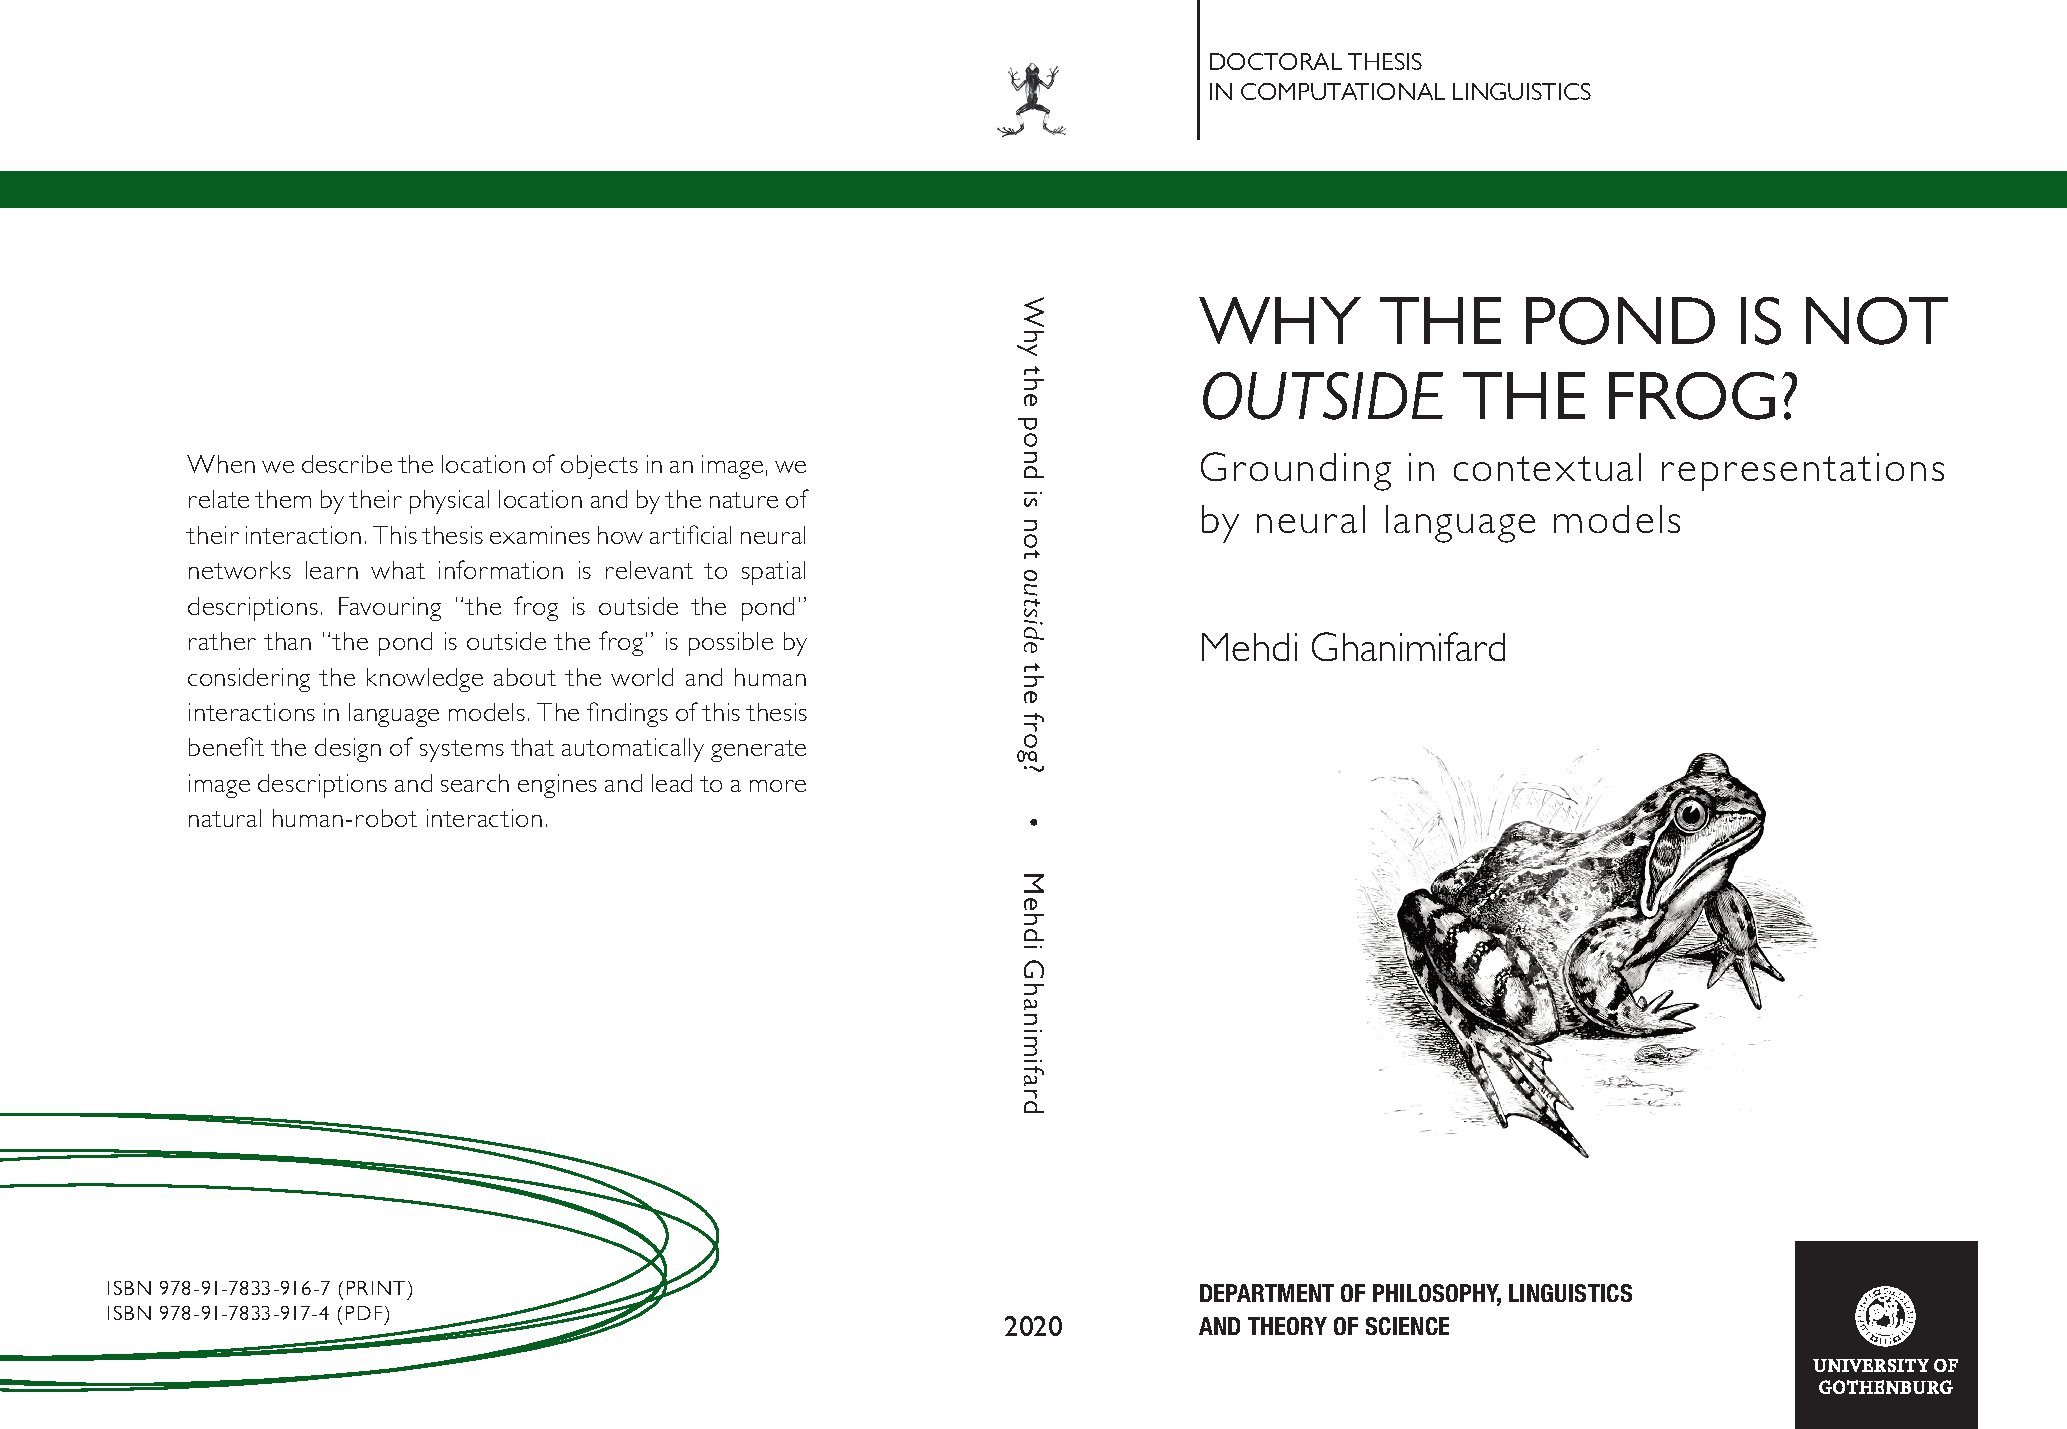
\includepdf[fitpaper,trim=185mm 0mm 0mm 0mm]{gfx/cover/cover-digital.pdf}
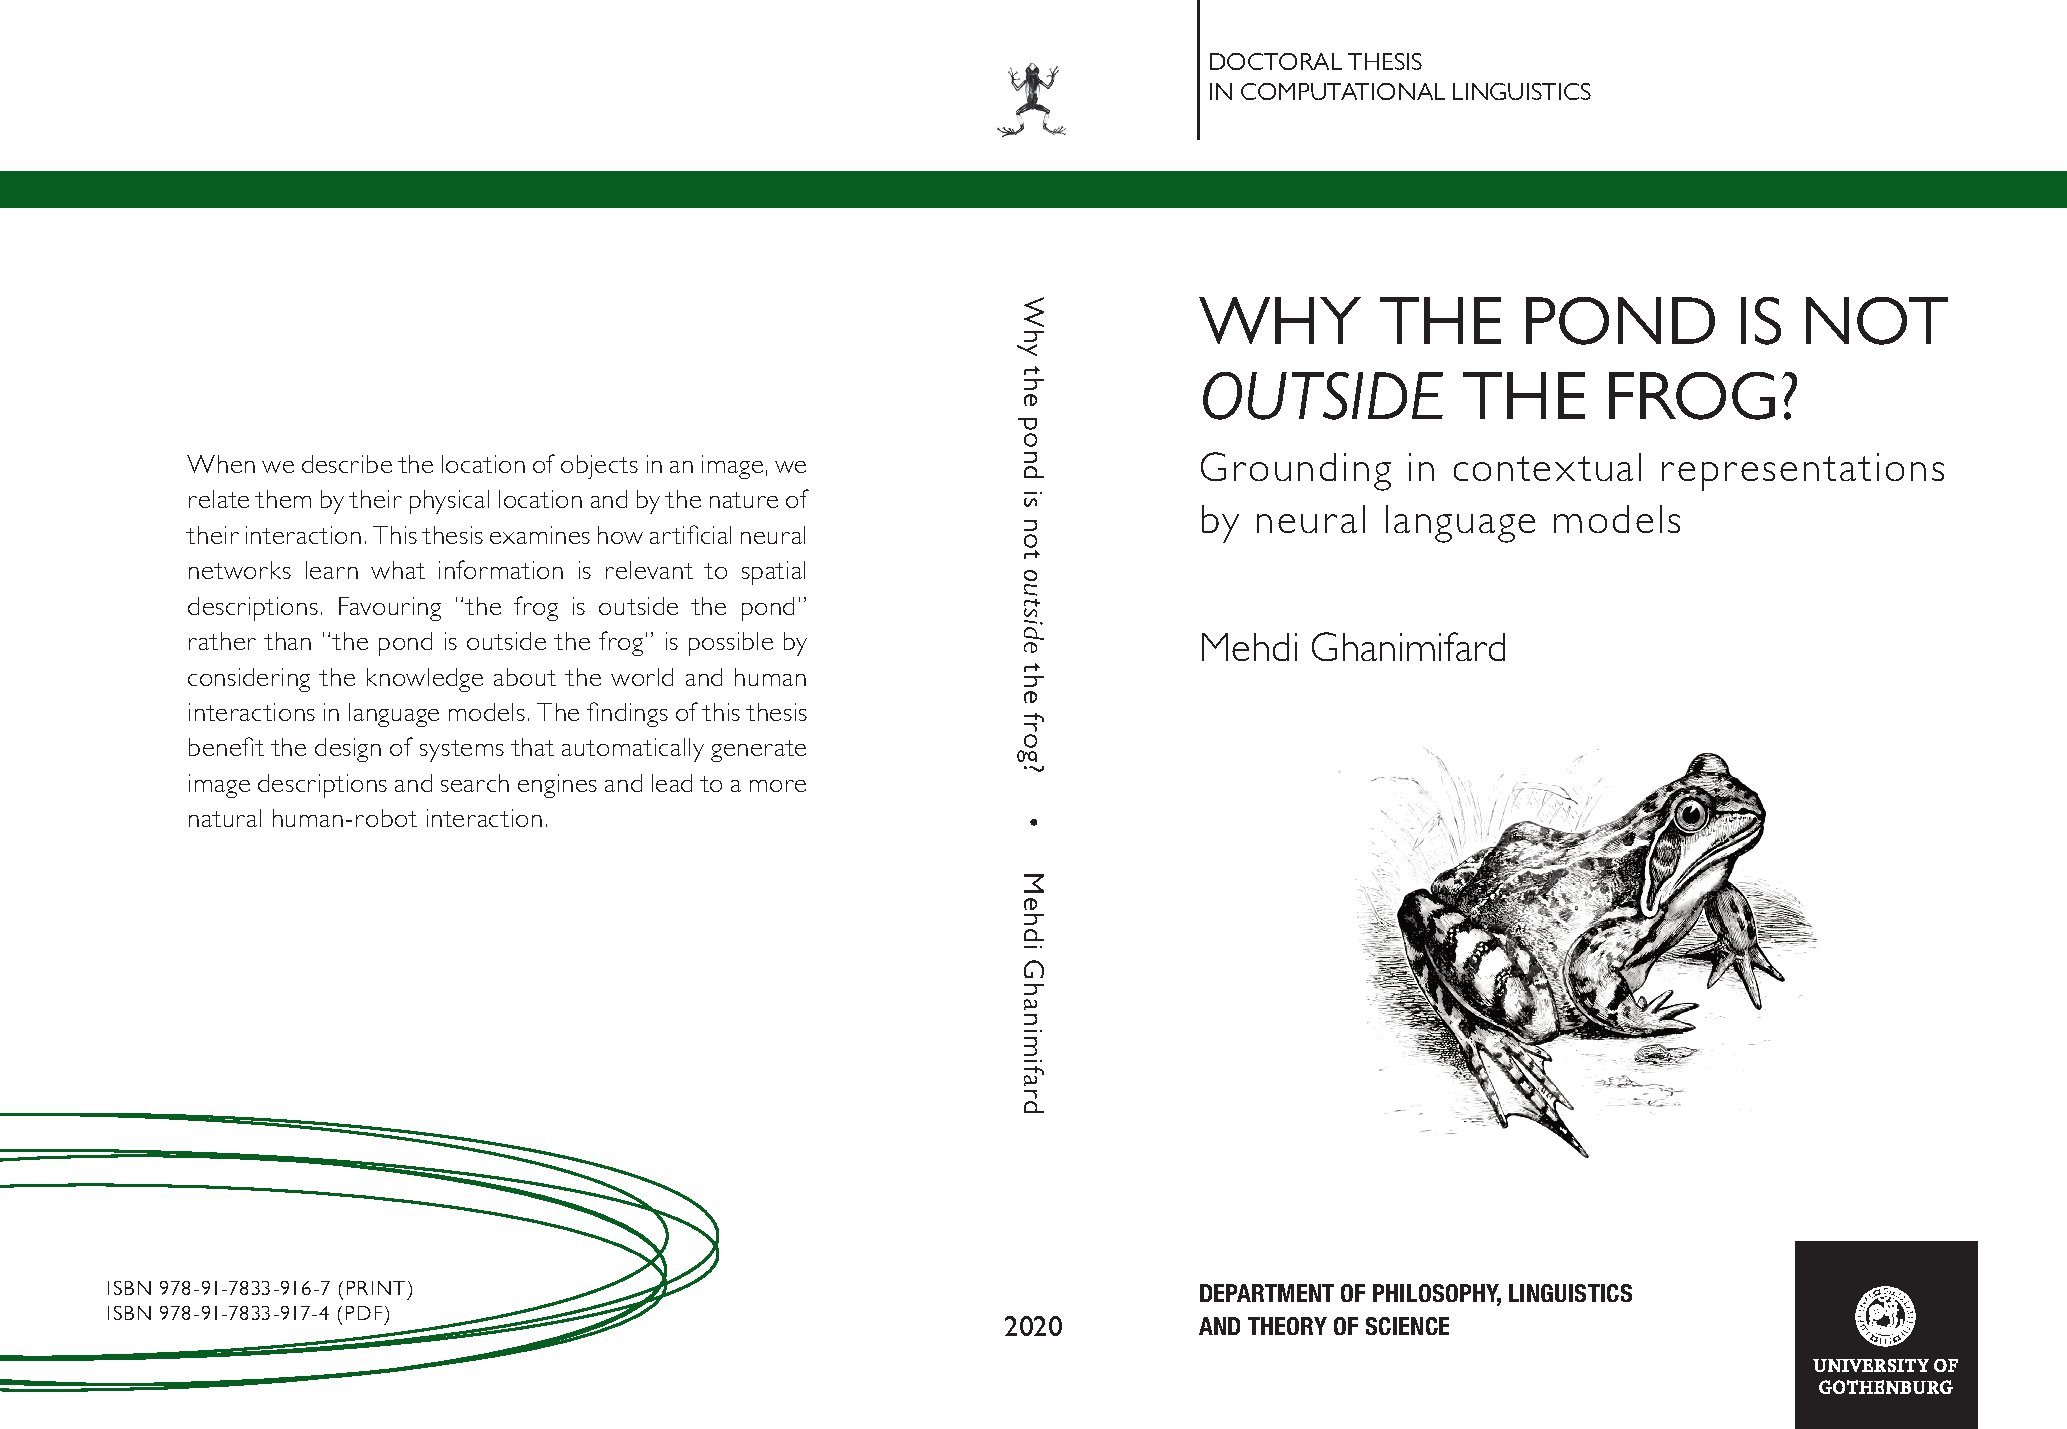
\includepdf[fitpaper,trim=0mm 0mm 185mm 0mm]{gfx/cover/cover-digital.pdf}
\setcounter{page}{1}
\fi

\begin{titlepage}
	\pdfbookmark[0]{Cover}{Cover}
	\flushright
	\hfill
	\vfill
	{\centering\LARGE\tgherosfont\thesisTitle \par}
	\vfill
	\flushright
\end{titlepage}


\begin{titlepage}
	\pdfbookmark[0]{Titlepage}{Titlepage}
	\tgherosfont
	\centering

	\vfill
	{\large\thesisSubject} \\[5mm]
	{\LARGE\thesisTitle \\[25mm]}
	
	\vfill
	
	{\Large \thesisName} \\[55mm]

	\vfill
	\textsf{\thesisUniversityDepartment} \\
	\textsf{\thesisUniversityGroup} \\ [10mm]
	\vfill

\includegraphics[width=6cm]{gfx/gu/LO_GUeng_cenSV.eps} \\
\thesisDate \\

\end{titlepage}


\hfill
\vfill
{
	\small
	\textbf{\thesisName} \\
	\textit{\thesisTitle} \\
	\thesisSubject, \thesisDate \\
	Main supervisor: \thesisFirstSupervisor \\[1.5em]
	\textbf{\thesisUniversity} \\
	\thesisUniversityDepartment \\
	\thesisUniversityStreetAddress \\[1.5em]
	The cover drawing from `{The Common Frog}' by \cite{thecommonfrog1881}. Not in copyright, scanned at Harvard University, Museum of Comparative Zoology, Ernst Mayr Library. \\
	The cover designed by Boshra Khoshnevis \\[1.5em]
	The research reported in this thesis was supported by a grant from the Swedish Research Council (VR project 2014-39) for the establishment of the Centre for Linguistic Theory and Studies in Probability (CLASP) at the University of Gothenburg.\\[1.5em]
	ISBN: \thesisISBNPrint\ (PRINT) \\
	ISBN: \thesisISBNPDF\ (PDF) \\[1.5em]
	Part I of the publication is also available in full text at: \\
	\url{http://hdl.handle.net/2077/64095}
}
		%
\cleardoublepage

\pagestyle{plain}				%
\pdfbookmark[0]{Abstract}{Abstract}
{\usekomafont{chapter}Abstract}
\label{sec:abstract:abstract}

In this thesis, to build a multi-modal system for language generation and understanding, we study grounded neural language models. 
Literature in psychology informs us that spatial cognition involves different aspects of knowledge that include visual perception and human interaction with the world. This makes spatial descriptions a compelling case for the study of how spatial language is grounded in different kinds of knowledge.
In seven studies, we investigate \emph{what} and \emph{how} neural language models (NLM) encode spatial knowledge. 

In the first study, we explore the traces of functional-geometric distinction of spatial relations in uni-modal NLM.
This distinction is essential since the knowledge about object-specific relations is not grounded in the visible situation. 
Following that, in the second study, we inspect representations of spatial relations in a uni-modal NLM to understand how they capture the concept of space from the corpus.
The predictability of grounding spatial relations from contextual embeddings is vital for the evaluation of grounding in multi-modal language models.
On the argument for the geometric meaning, in the third study, we inspect the spectrum of bounding box annotations on image descriptions. 
We show that less geometrically biased spatial relations are more likely to deviate from the norm of their bounding box features.
In the fourth study, we try to evaluate the degree of grounding in language and vision with adaptive attention.
In the fifth study, we use adaptive attention to understand if and how additional bounding box geometric information could improve the generation of relational image descriptions. 
In the sixth study, we ask if the language model has an ability of systematic generalisation to learn the grounding on the unseen composition of representations.
Then in the seventh study, we show the potentials in using uni-modal knowledge for detecting metaphors in adjective-nouns compositions.

The primary argument of the thesis is built on the fact that spatial expressions in natural language are not always grounded in direct interpretations of the locations. 
We argue that distributional knowledge from corpora of language use and their association with visual features constitute grounding with neural language models. 
Therefore, in a joint model of vision and language, the neural language model provides spatial knowledge that is contextualising the visual representations about locations. 





\clearpage
{\usekomafont{chapter} Sammanfattning (Abstract)}
\label{sec:abstract:abstract-svenska} 

I denna avhandling, för att bygga ett multimodalt system för språkgenerering och förståelse, studerar vi förankrade neurala språkmodeller.
Litteratur i psykologi informerar oss om att rumslig kognition involverar olika aspekter av kunskap som inkluderar visuell uppfattning och mänsklig interaktion med världen. Detta gör att rumsliga beskrivningar är ett bra fall för att studera hur rumsligt språk är förankrat i olika typer av kunskap.
I sju studier undersöker vi \emph{hur} neurala språkmodeller (NLM) kodar rumslig kunskap, och \emph{vad} de kodar.

I den första studien undersöker vi spåren av den funktionella-geometriska distinktion av rumsliga relationer i unimodala NLM.
Denna distinktion är väsentlig eftersom kunskapen om objektspecifika relationer inte är baserad i den synliga situationen.
Därefter, i den andra studien, inspekterar vi representationer av rumsliga relationer i unimodala NLM för att förstå hur de representerar begreppet rymd från en korpus.
Förutsägbarheten av grundläggande rumsliga relationer från kontextuella representationer är avgörande för utvärderingen av förankring i multimodala språkmodeller.
I den tredje studien undersöker vi argument för den geometriska betydelsen genom att inspektera spektrumet av avgränsningsruteannoteringar för bildbeskrivningar.
Vi visar att geometriska relationer med en mindre grad av rumslighet är mer benägna att avvika från normen av avgränsningsfunktionens särdrag.
I den fjärde studien försöker vi utvärdera graden av förankring i språk och syn med adaptiv uppmärksamhet.
I den femte studien använder vi adaptiv uppmärksamhet för att förstå om och hur ytterligare geometrisk information om avgränsningsrutorna kan förbättra generationen av relationella bildbeskrivningar.
I den sjätte studien frågar vi om språkmodeller har en systematisk generaliseringsförmåga att lära sig förankring av osedda sammansättningen av representationer.
Sedan i den sjunde studien visar vi att unimodal kunskap har potential för att upptäcka metaforer i adjektiv-substantivkompositioner.

Avhandlingens huvudargument bygger på det faktum att rumsliga uttryck i naturligt språk inte alltid är baserade på direkta tolkningar av platser.
Vi hävdar att distributionell kunskap från korpusar om språkbruk och deras associering med visuella funktioner utgör förankring för neurala språkmodeller.
Därmed, en modell som använder både visuell information och språk, tillhandahåller neurala språkmodeller rumslig kunskap som kontextualiserar visuella representationer av platser.


\clearpage
{\usekomafont{chapter}List of Publications}\label{sec:abstract:publications} \\



\paragraph{Study 1}
Simon Dobnik, Mehdi Ghanimifard and John Kelleher. 
Exploring the Functional and Geometric Bias of Spatial Relations Using Neural Language Models.
\textit{In Proceedings of the First International Workshop on Spatial Language Understanding, pp. 1-11. 2018.}

\paragraph{Study 2}
Mehdi Ghanimifard and Simon Dobnik. 
\emph{What} a neural language model tells us about spatial relations. 
\textit{In Proceedings of the Combined Workshop on Spatial Language Understanding (SpLU) and Grounded Communication for Robotics (RoboNLP), pp. 71-81. 2019.}

\paragraph{Study 3}
Simon Dobnik and Mehdi Ghanimifard.
Spatial descriptions on a functional-geometric spectrum: the location of objects. 
\textit{Preprint - under review, 2020.}

\paragraph{Study 4}
Mehdi Ghanimifard and Simon Dobnik. 
Knowing When to Look for What and Where: Evaluating Generation of Spatial Descriptions with Adaptive Attention. 
\textit{The European Conference on Computer Vision (ECCV) Workshops, pp. 153-161. Springer, Cham, 2018.}

\paragraph{Study 5}
Mehdi Ghanimifard and Simon Dobnik.
What Goes Into A Word: Generating Image Descriptions With Top-Down Spatial Knowledge
\textit{In INLG 2019-12th International Conference on Natural Language Generation-Long papers. 2019.}

\paragraph{Study 6}
Mehdi Ghanimifard and Simon Dobnik. 
Learning to Compose Spatial Relations with Grounded Neural Language Models. 
\textit{In IWCS 2017-12th International Conference on Computational Semantics-Long papers. 2017.}

\paragraph{Study 7}
Yuri Bizzoni, Stergios Chatzikyriakidis and Mehdi Ghanimifard. 
``Deep'' Learning: Detecting Metaphoricity in Adjective-Noun Pairs.
\textit{In Proceedings of the Workshop on Stylistic Variation, pp. 43-52. 2017.}


		%
\cleardoublepage
\pdfbookmark[0]{Acknowledgement}{Acknowledgement}
\chapter*{Acknowledgement}
\label{sec:acknowledgement}
This collection of articles was a result of a long journey that started in 2015 when I joined the PhD program at CLASP. Producing such a piece is not a one-person job. I was fortunate to have the support of my supervisors, colleagues, friends and family along the way.

First of all, I would like to recognize the invaluable assistance of my supervisors. 
I want to express my most profound appreciation to Simon Dobnik, my primary advisor, for his steady support of my trembling steps on this path. A large body of this work became possible with his direct guidance. 
I wish to acknowledge the efforts of Staffan Larsson, my second advisor, whose feedback helped me at various times during this project. 
I am incredibly grateful to John Kelleher, my third advisor, our long passionate conversations shaped many ideas presented here.
In addition to the help I received from supervisors, I was lucky for being able to seek advice from other fantastic people. 
I am indebted to Richard Johansson for his counselling which led me to apply for the PhD program. I had the privilege to receive his support since I was a master student. 
I am also grateful to Stergios Chatzikyriakidis for his encouraging feedback. I have always been able to rely on his friendly advice.
Also, I want to thank Lena Eriksson for her counselling. Her thoughtful advice proved to have a significant influence on the success of my studies.
I wish to thank, Desmond Elliott, my thesis assessor, for his constructive criticism and helpful feedback on an earlier version of the thesis.

I want to extend my sincere thanks to friends and colleagues for building such an excellent social and research environment. 
Shalom Lappin, for his unparalleled support and care;
Robin Cooper, for sharing extensive knowledge in our bi-weekly meetings at the language and perception reading group; 
Jean-Philippe Bernardy, for his constructive advice from time to time;
Yuri Bizzoni, for being a colleague and a friend with a significant positive atmosphere around him. Also, thanks to Johan Gross and Julia Forsberg, with Yuri, we had a relaxed PhD life at the office! 
Same regards to Adam Ek and Vidya Somashekarappa my officemates for almost a year. Although we only shared office for a short period, we made unforgettable memories. I literally received a collection of life lessons from Vidya and Adam after their thoughtful prank! 
I also wish to thank all the incredible people who made Dicksonsgatan 4 like a family house for me. Haris Themistocleous, Chris Howes, Ellen Breitholtz, Sharid Loáiciga, Asad Sayeed, Sandro Maskharashvili, Rasmus Blanck, Wafia Adouane, Vlad Maraev, Bill Noble, Sylvie Saget, Kathrein Abu Kwaik, Susanna Myyry, Iines Turunen, Aram Karimi. We had a lot of meaningful spontaneous conversations in the kitchen, corridors and the meeting room. I learned something memorable from each of you. I won't miss a chance if I get to work with you again. 

The extent of the fantastic colleagues that I wish to thank them for their company goes beyond the circle of CLASP, at GU and Chalmers. Conversation with these friendly faces kept me on the track! I want to thank Mio Cibulka, Leila El-Alti, Richard Endörfer, David Alfter, Luis Nieto Piña, Ildikó Pilán, Prasanth Kolachina, Herbert Lange.  

I cannot begin to express my thanks to my family and friends whose support cannot be overestimated. These extraordinary people kept me sane during my PhD life. In Sweden, I had incredible times with Alireza Pazirandeh, Ala Pazirandeh, Niklas Arvidsson and My Högblom. 
I wish to thank my sisters, Marzieh and Mona, and my mother and father, Shokoufeh and Siamack, for profound belief in my work and my abilities. 

Lastly, I would like to thank my wife, Boshra Khoshnevis (without forgetting the help of Biloo and Ghoughies). She is the reason that kept me going on. The completion of my dissertation without her support would not be possible.



 %
\cleardoublepage
\setcounter{tocdepth}{1}		%
{\hypersetup{
	colorlinks=true,
	citecolor=ctcolorblack,
	linkcolor=ctcolorblack,
	urlcolor=ctcolorblack
}\tableofcontents}
\cleardoublepage

\pagenumbering{arabic}			%
\setcounter{page}{1}			%
\pagestyle{maincontentstyle} 	%

\part{Thesis Frame}
\chapter{Introduction}
\label{sec:intro}

The success of a class of machine learning algorithms in a wide variety of computer vision tasks led to the emergence of the deep learning paradigm over the past decade. 
This transformation in computer vision has affected the design and application of perceptual systems in other domains, such as human-robot interactions and computational linguistics. 
Designing a system based on a data-driven module, such as a neural network classifier, would be challenging without a proper explanation of how the system would reason in situated environments. 
The potential applications of deep neural networks and questions about different models and how to apply them initiated and motivated this research.
In this chapter, we describe the aims of the thesis, the research questions and the objectives.
Then, we briefly address the contributions and findings of the studies within this thesis.
In the next chapters, we provide more detailed background information.

\section{Aims}
\label{sec:intro:aims}
The main objective of this thesis is to pave the way for the development of language generation and language understanding systems with deep neural networks that are grounded in both linguistic and visual inputs.
Several use cases of such systems involve spatial language, including automatically describing the location of objects or locating objects based on a description of their whereabouts.
These use cases have guided this research to focus on spatial language as an original puzzle in the domain of computational linguistics. 

Our goal of building such systems yielded several challenges and fundamental questions about learning representations using deep neural networks.
Therefore, the primary aims of the thesis are to assess and investigate the application of neural networks in automatically learning multi-modal representations and the grounding of linguistic units in such representations.



\section{Research questions}
\label{sec:intro:questions}

\paragraph{Q1: What spatial knowledge is learned in neural language models?} 
A fundamental question about the representation of modalities is whether these modalities are sufficient for solving the relevant tasks. Language modelling yields several other questions about the encoding of knowledge. 
Is the knowledge encoded in these modalities extractable using specific learning algorithms and models?
In the context of spatial language, is there appropriate geometric knowledge in representations that can be learned with neural models (such as convolutional neural networks)? 
Is the geometric knowledge in relevant modalities enough to understand or generate a spatial description of a situation?

\paragraph{Q2 How are spatial descriptions associated with spatial knowledge?} 
The measure of success in a data-driven inference cannot be just the accuracy of correct predictions. 
To have a valid data-driven procedure, there must be an explanation of which evidence is used to conclude the decision. 
Therefore, we ask the following questions. 
How do different modalities contribute to a grounded neural language model? 
How much do visual inputs affect the results in comparison to language inputs? 
What is the balance between the contributions of different modalities? Why do different modalities contribute differently to the performance of the model?

\paragraph{Q3 Is there a systematic generalisation?} 
The assessment of learning with neural networks cannot be limited to the ability of the system to perform specific tasks in specific examples. 
This question is often asked in the form of learned compositionality. 
We investigate the generalisability of learning outcomes by looking at learned representations. 
To what degree are the expected structures, compositions and relations in linguistic and visual-cognitive representations learned with neural networks? 
If unexpected relations within neural representations emerge from learning distant tasks, such as language modelling, we need to show if the learned representations imposed from the data are transferable knowledge or if the relations are intrinsic to the neural structures and can be generalised.
If there are intrinsic neural structures that capture the compositional relations in neural representations, we ask if these structures are aligned with expected structures. 
For example, if a two-arity relation is not symmetric, is the order of arguments preserved in learned representations?
Is the order in neural structures aligned with the expected order?
















\section{Contributions and findings}
\label{sec:intro:contributions}





Our findings are distributed over seven studies. 
In the first three studies
\citep{dobnik-etal-2018-exploring,ghanimifard-dobnik-2019-neural,dobnik-ghanimifard-2020-geo},
we inspect unimodal neural language models and the geometric features of bounding boxes to see what latent knowledge on spatial relations is encoded in the models and data \textbf{(Q1)}. 

Then, in studies 4 and 5  \citep{ghanimifard2018knowing,ghanimifard-dobnik-2019-what},
we examine the contributions of visual features and contextual embeddings from a language model in generating image descriptions. We show that the contributions of visual features in producing spatial relations are lower than nominal parts of speech. We also show that top-down localisation has the highest contribution to performance compared to any other top-down feature representation \textbf{(Q2)}.  
In study 5, the question about top-down representations in neural networks resolves whether the intrinsic structures in neural networks affect learning \textbf{(Q3)}. 

The last two studies 
\cite{ghanimifard-dobnik-2017-learning,bizzoni-etal-2017-deep}, focus on the capability of neural language models to learn compositional knowledge. We show that, when using neural networks as the composition function, the models can generalise from limited samples of language use to new word compositions \textbf{(Q3)}. 
In study 6, we found that composing unseen word sequences and decomposing unseen single word representations are possible if the neural language model is trained with enough coverage of vocabulary.
However, this is dependent on combinatorial properties and the complexity of compositional meaning \textbf{(Q2)}.
In study 7, we found that distributional knowledge from neural language models, abstracted from visual/sensory grounding, can recognise metaphors.
This finding is consistent with our findings in study 2 \textemdash  that unimodal language models can capture spatial knowledge in distributional patterns \textbf{(Q1)}.

	
\section{The thesis frame}

This dissertation consists of two parts, the thesis frame and the studies. The first part comprises a synthesis of ideas, background case studies, concepts, a summary of studies and the conclusions of the thesis (chapters 1 to 5). The second part comprises the seven articles of the research project (chapters 6 to 12). 

In chapter 2, we briefly explore the background of spatial language in image descriptions. In chapter 3, we extensively discuss the concept of modelling meaning representations with neural networks. chapter 4 summarises the seven studies in connection with the research questions and their findings. Finally, chapter 5 provides the final summary and discussion of the thesis findings and its connection to the published studies.
\chapter{Spatial Expressions In Image Descriptions}
\label{sec:spatial}


The importance of spatial language is embedded in fundamental domain questions about parsing visual sensory inputs into meaningful representations. 
In its purest form, the individuation of objects would be a spatial cognition task; 
to recognise where objects begin and where they end in space, how their parts are spatially composed and how the spatial properties (including shapes and locations) interact with each other.  
In chapter 1, we stated that the use cases of grounded language generation and understanding brought us to the study of spatial language. In a large body of work on referring expression generation 
\citep{DaleReiter:1995,Krahmer:2011aa} with applications that describe scenes \citep{Viethen:2008aa} and images  \citep{Mitchell:2012aa,elliott2013image}, describe visible objects  \citep{mitchell-etal-2013-generating} and engage in human-robot dialogue \citep{kelleher-kruijff-2006-incremental,Dobnik:2009dz}, spatial grounding language is inseparable from the tasks. 
In this chapter, we discuss the relevant topics and concepts regarding how human language can describe the space, the location of objects and the relation between them in an image.

\section{Spatial expressions}
\label{sec:spatial:expressions}
There are many ways to describe a situation and convey information about the location of important matters. The most direct form of denoting the location of objects in natural language is to use \emph{locative expressions}. 
The simplest type of locative expression is composed of three constituents \textemdash  a locative preposition and two noun phrases.
One of the noun phrases is the subject of the preposition and the other is the object. 
\begin{figure}[t]
	\centering
	\begin{minipage}{0.6\linewidth}
		\begin{itemize}[leftmargin=0.1cm,itemsep=1em]
			\item[] The~\textit{frog~next~to}~the~\textit{pond}.
			\item[] The~\textit{frog}~is~\textit{next~to}~the~\textit{pond}.
			\item[] There~is~a~\textit{frog~next~to}~the~\textit{pond}.
			\item[] The~\textit{frog~next~to}~the~\textit{pond}~is~watching~us.
		\end{itemize}
	\end{minipage}%
	\begin{minipage}{0.4\linewidth}
		\centering
		\fbox{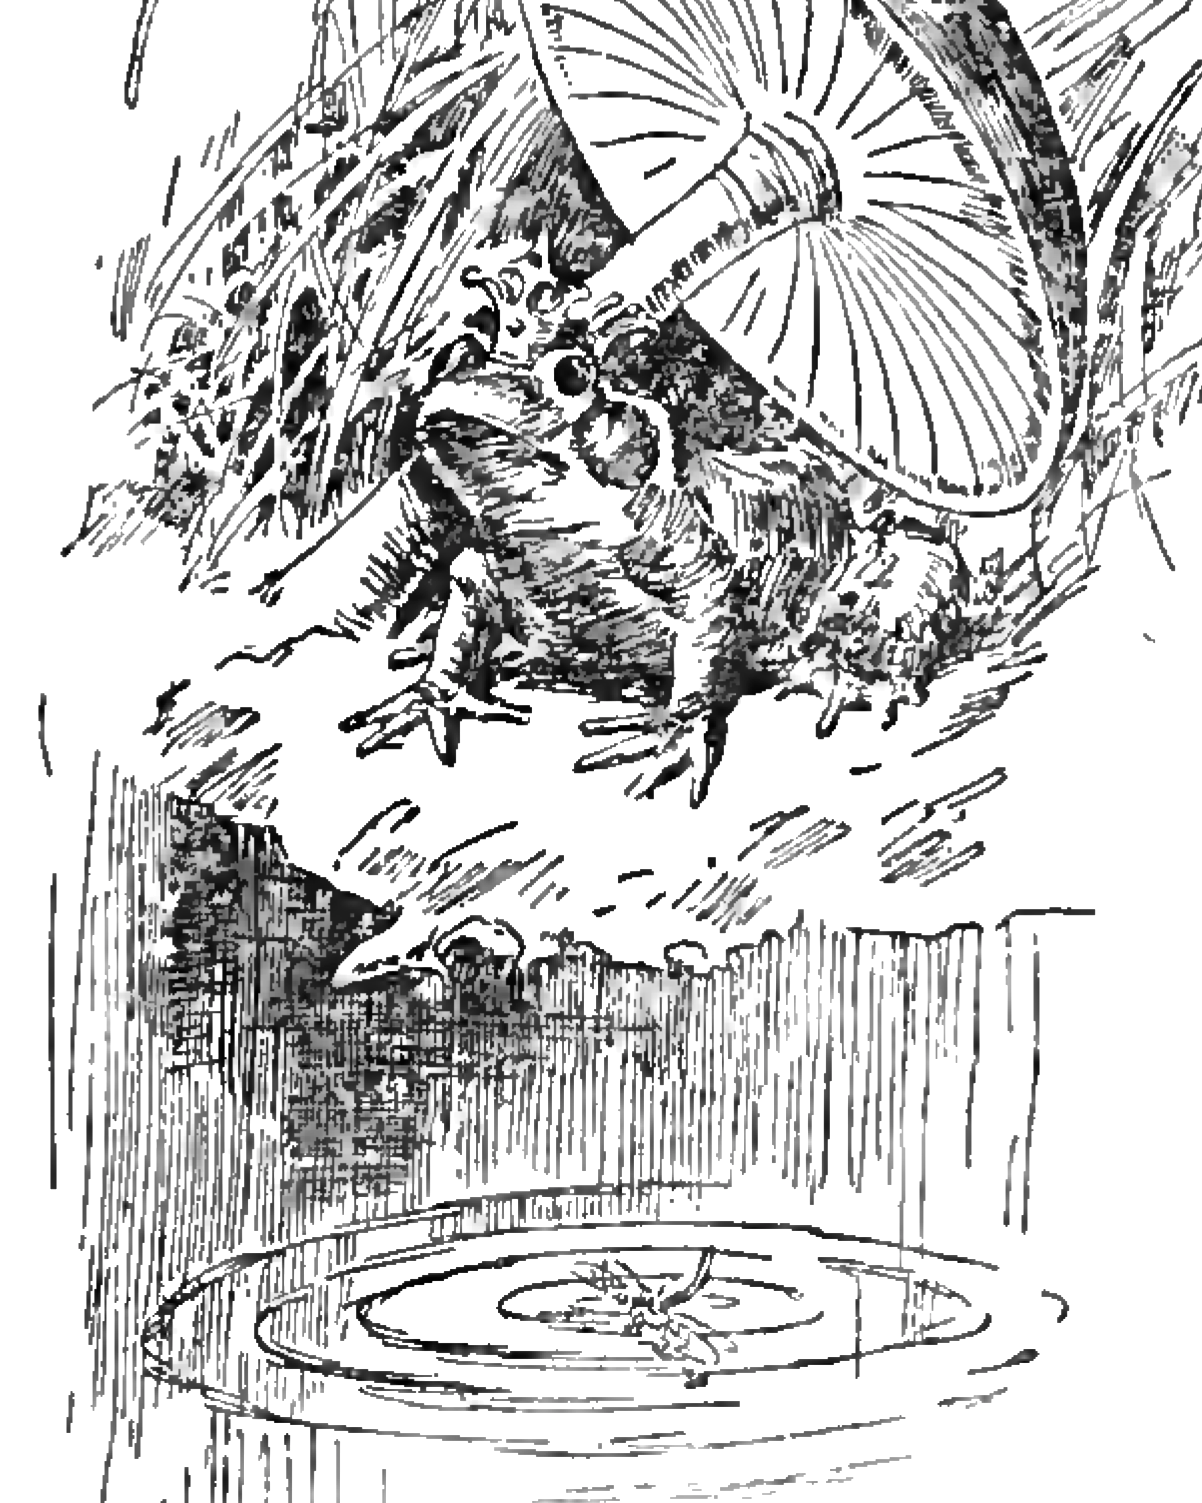
\includegraphics[width=0.78\linewidth]{gfx/frog-prince.png}\footnote{The drawing from \emph{Grimm's Fairy Tales} by \cite{grimmsfairytales1899}}}
	\end{minipage}%
	\caption{Describing the location of target and landmark \textemdash  $\langle$ \textit{frog},\textit{next~to},\textit{pond}$\rangle$.}\label{fig:frog-next-to-pond}
\end{figure}
For example, in `the~frog~next~to~the~pond' the preposition  `next~to' describes the location of the subject `the~frog' with respect to the object `the~pond'. The subject/object are also known by different names, such as \emph{referent}/\emph{relatum} \citep{Miller-JohnsonLaird:1976}, \emph{figure}/\emph{ground} \citep{Talmy:1983} or \emph{located object}/\emph{reference object} \citep{herskovits1986language,Gapp:1994:BasicMeanings,Dobnik:2009dz}.
In this work, we refer to them as  \textsc{Target}/\textsc{Landmark}. 
When referring to a situation with the structure  $\langle\textsc{Target},\textsc{Relation},\textsc{Landmark}\rangle$, 
the expression may be combined with a copulative verb, an existential quantifier or other additional information  (Figure~\ref{fig:frog-next-to-pond}).

In English, there are a small class of words with meanings that denote spatial relations between targets and landmarks. This includes simple words (\emph{on}, \emph{in}, \emph{over}, \emph{under}) and compound phrases (\emph{on top of}, \emph{to the left of}, \emph{to the right of}, \emph{in front of}, and etc.)
Some of these relations are compositional, which means they can be combined to produce new relations (\emph{above} and \emph{far from}). 
Based on the list of prepositions in \citep{landau1993whence}
and alternative compositional and compound relations discussed in  \cite[p.~156]{herskovits1986language}, we created a dictionary of $75$ spatial relations. Considering their alternative forms, with a minor difference in their spatial sense, they constitute $1,194$ entries\footnote{The source code to generate the collection of multi-words expressions is available in the online repository of published studies including \url{https://github.com/GU-CLASP/functional-geometric-lm}.} (Table~\ref{tab:ch2:vocab}). 
For example, `\emph{to the left of}' could be one form of several possible alternative multi-words with close spatial meaning:
\begin{itemize}[topsep=0em,itemsep=0em,partopsep=0em,parsep=0em]
	\item \emph{\{at/on/in/to/by\} the left \{\{hand\} side\} of} $\to$ \emph{to the left of}. 
\end{itemize}

	
\begin{table}[t]
	\begin{tabular}{|lllll|}
		\hline
		about         & above         & across        & after         & afterward     \\
		against       & ago           & along         & alongside     & amid          \\
		among         & apart         & around        & at            & away          \\
		back          & backward      & before        & behind        & below         \\
		beneath       & beside        & between       & bottom        & by            \\
		down          & downstairs    & downward      & during        & east          \\
		from          & front         & here          & in            & inside        \\
		into          & inward        & left          & near          & nearby        \\
		next          & north         & off           & on            & onto          \\
		out           & outside       & outward       & over          & parallel      \\
		perpendicular & right         & side          & sideways      & since         \\
		south         & there         & through       & throughout    & to            \\
		together      & top           & toward        & under         & underneath    \\
		until         & up            & upon          & upstairs      & upward        \\
		via           & west          & with          & within        & without       \\
		\hline
	\end{tabular}
	\vspace{0.5em}
	\caption{The vocabulary of $75$ spatial relations from \cite{landau1993whence} and \cite{herskovits1986language}.}\label{tab:ch2:vocab}
\end{table}


\section{Functional/geometric meaning}
\label{sec:spatial:functional}
Expressing location and describing space is not limited to the prepositional relations in spatial expressions. Other verbs in referring expressions can indicate the relative location between subject and object. With different degrees, these relations might have a strong or weak association with the location of the subject and object. 
For example, `\emph{ride}' entails a specific spatial configuration between the subject and the object, depending on their shape. 
Other relations, such as `\emph{touch}', `\emph{sit on}', and `\emph{jump over}' indicate a specific spatial configuration of subject and object.
Nevertheless, their direct meaning is not just the location of objects; it indicates other kinds of relations, which consequently entail specific spatial arrangements. 

In the same way, the meaning of spatial prepositions is not purely geometrical; it entails other relations and associations between subject and object that are functional. 
The relation  `\emph{over}' does not just describe a geometric location; it also indicates a function \textemdash  the subject provides protection or shelter for the object/s.
The functional sense of relations includes specific interactive relations between entities that are not dependent on the location and spatial configurations.

A simple representation of the geometric sense of relations is based on the acceptability ratings of individual locations with respect to the landmark. 
\cite{logan1996computational} suggest that the mental representation of a geometric meaning could be a template projection of locations on a map, where the landmark is in the middle and each location has its degree of acceptability for the target object. 
A study on location acceptabilities for different prepositions shows that each spatial preposition has a different degree of dependency on object-specific relations  \citep{coventry2001interplay}.
The meaning of each relation is an interplay between the functional and geometric relations of two objects.
For instance, \emph{`above'} has both geometric locational meaning and functional sense. 
When it is used in different context it can have different degree of functional and geometric acceptability.
Spatial relations in natural language have a spectrum of geometricity, with different degree of favouring geometric bias or functional bias. 
Another way to study the object-specific sense of relations is to consider the distributional dependency between relations and objects in image descriptions \citep{Dobnik:2013aa,Dobnik:2014ab}.
In our studies, we consider these aspects of by examining language models.

\section{Image descriptions}
\label{sec:spatial:image}
In a simple \emph{show-and-tell} task, when provided an image, the agent must generate a description of the image. 
Since the early works on human-robot interactions, this task became the centre of interests for natural language grounding \citep{roy2002learning}. 
In recent years, several large datasets have been developed, in which crowd-sourced human annotators describe images from freely available datasets of photographed scenes over the Internet.

\paragraph{Datasets}
Common datasets of image caption tasks, such as MSCOCO  \citep{lin2014microsoft} with more than 300,000 images and Flickr30k  \citep{flickr30k} with 30,000 images, each provide five alternative descriptions per image. 
However, the variation and number of geometric spatial relations in the dataset is limited;
`\emph{to the left of}' and `\emph{to the right of}' are rarely used in the dataset. 
On the other hand, the Visual Genome \citep{krishna2017visual} provides 50 region descriptions and triplet annotations per image, for a total of over 108,000 images. 
The annotation schema, in this case, was slightly different from captioning, as it asks annotators to describe specific parts of the images or the relation between two object areas in the images. 
In this dataset, description and relation annotations are associated with relevant bounding boxes in the image.


\paragraph{Grounding spatial descriptions}
Both generating and understanding a spatial description with three components \textemdash  $\textsc{Target}$, $\textsc{Relation}$, $\textsc{Landmark}$ \textemdash  requires several types of knowledge:
 (1) object identification,
 (2) comprehension of geometric configuration,
 (3) capturing object-specific relations between objects and 
 (4) a frame of reference for projective relations `\emph{to the right of}' and `\emph{below}'.
When people describe image contents, they commonly use spatial expressions. 
A scene can be described correctly using any spatial relation fitting the same objects depending on the intent of the speaker.
However, the image description task may use the knowledge about the scene in a specific way.%
Precisely, object identification and the capture of object-specific relations in the picture might be enough to describe an image with spatial expressions.

\section{Summary}
\label{sec:spatial:summary}
In this chapter, we described the concept of locative expressions and its connection with image descriptions. 
Spatial relations denote locations in scenes. However, their meaning, to some extent, is also dependent on object-specific relations. 
In our studies on grounding spatial descriptions, we will use datasets of images with descriptions, including MSCOCO\citep{lin2014microsoft}, Flickr30k\citep{flickr30k} and Visual Genome \citep{krishna2017visual}.
\chapter{Modelling And Meaning Representation}
\label{sec:concepts}


In this chapter, we address the concepts and the theoretical framework for modelling meaning with uncertainty and grounding natural language in multi-modal representations.

\section{Terminology of modelling}
\label{sec:concepts:model}
Whenever we need to make a systematic prediction based on observations and evidence, we use a set of assumptions. 
A \emph{model} is the encoding of these assumptions in the form of a function. 
This function takes given evidence as input and produces the prediction as an output. Formally, modelling $y$ based on $x$ with the function $f$ would be as follows:

\begin{equation}
y = f_{\Theta}(x)
\end{equation}
\noindent where $f_{\Theta}$ is called the \emph{model function}, which is parametrised with $\Theta$. 

The parameters are part of the assumption about the model function. 
For example, by assuming the rules of physics, the position of a falling object at a specific time in the future can be modelled given the current evident position of the object. 
However, the formula of the location still requires the important parameters of velocity and acceleration of the object in the model. 
More often, determined prediction of an outcome is not enough. We need to associate each prediction with an uncertainty measure. 
Such a model is a \emph{probabilistic model}. 
Instead of modelling the predictable outcome, a measure of uncertainty for any possible outcome is modelled; the density of possible outcomes is conditioned with the observable evidence.
\begin{equation}\label{eq:probabilistic_model}
\mathrm{Pr}( Y=y | X=x ) = f_{\Theta}(y, x)
\end{equation}
\noindent where $f_{\Theta}$ is the model function, which assigns a degree of uncertainty for predicting $y$ grounded on an observable $x$. To simplify the probability annotations, we do not write the complete propositions ($Y=y$); instead, we use shorthand \textemdash  $\mathrm{Pr}( y | x )$.
Commonly, the probability distributions used in this work are categorical, in which $Y$ is a bounded discrete vector of the items. Therefore, the common implementation of function $f_{\Theta}$ is conducted using a module with a vectorised output the same size as $Y$:
\begin{equation}\label{eq:probabilistic_model_module}
f_{\Theta}(y, x) = \mathtt{modules}(x)[y]
\end{equation}
\noindent where $y$ is a category in distribution, the output of $\mathtt{modules}(.)$ is a vector with the size of all possible categories and the square bracket annotation $[y]$ indicates a lookup operation to select the value for $y$-key.

Representing assumptions about the future in a function requires a \emph{framework of modelling} to acquire the model function. 
A constructive \emph{proof}, a search algorithm over a class of functions or its parameters, is the path to building the model function from these assumptions.
When a set of data points drives the search algorithm, the process of fitting a function according to these data points is called \emph{learning} or \emph{training} the model.


\section{Modelling in deep neural networks}
\label{sec:concepts:dl}
In this work, we study the framework of artificial neural networks to encode and build the model function. 
\emph{Deep learning} (DL) and \emph{artificial neural networks} (ANN)
refer to a modelling framework in which a composition of differentiable functions form the model function.
The learning occurs through parameters of the function with the \emph{backpropagation algorithm}.
The backpropagation algorithm is a data-driven optimisation algorithm that uses a measure of error loss over the training data to gradually update the model parameters toward lower error. 
The differentiability of the loss enables this method to apply the chain rule of derivatives to aim the parameter updates toward reducing errors for the training data. 
In a nutshell, the critical assumptions needed to build a deep learning model are the assumed model function (the composition of modules or the neural network architecture), the assumption that the training dataset has relevant knowledge for the task and the assumption about the error function (the loss function).

There are several learning paradigms, such as supervised and unsupervised learning.
These distinctions mainly concern the difference in annotation on the training data, the error function and how they are related to the predictable variable of the model.
The most common paradigm is supervised learning, in which the training dataset is a set of annotated inputs and the predicted output of the model $D = \{(y_i, x_i)\}$.
Unsupervised learning, on the other hand, uses an unlabelled training dataset $D = \{x_i\}$.
The error function in these cases provides additional assumptions about how data points are internally connected. Any internal data structures that indirectly relate to the predictable outcome of the model could be the basis for an error function in unsupervised learning, such as unsupervised clustering of data points for a classification task without supervised data.

The most common loss function for deep learning models is the surprisal of the training data. The surprisal of a random variable ($X=x$) is defined as: 
$\bm{I}_X(x) = -\mathrm{log}(\mathrm{Pr}(X=x))$. 
With a given dataset, such as $D = \{(y_i, x_i)\}$ and a model function $f$, an ideal search algorithm for finds the best fitting parameters that minimise the loss:
\begin{align}
J_\Theta(f,D) &= \sum_{(y_i, x_i) \in D}{-\mathrm{log}(f_{\Theta}(y_i, x_i))} \\
\Theta &= \underset{\Theta}{\mathrm{argmin}} J_\Theta(f,D)
\end{align}
\noindent while the search algorithm looks for the best fitting parameters $\Theta$, there is usually more than one answer or there is no converging path to an acceptable error level with backpropagation. In the most straightforward form \textemdash  backpropagation in a \emph{gradient descent algorithm} \textemdash  the gradient of the error function with a pre-defined learning rate updates all parameters iteratively until the error converges to an acceptable threshold. 
To overcome technical difficulties in processing large datasets and parameter space, other variations of this algorithm may process data in batches, using \emph{stochastic gradient descent} and the momentum of past updates. 
For simplicity, each step of mini-batch training can be formulated as an updating operation for $\Theta$ parameters as follows: 
\begin{equation*}
\Theta = \Theta - \eta \cdot \nabla_\Theta J_\Theta(f; D_{batch})
\end{equation*}
\noindent
where $\eta$ is a hyper-parameter for the learning rate and $\nabla_\Theta$, is a notation for a stochastic deferential operation over every parameter in $\Theta$.

The concept of indirect learning from a function different from the goal prediction of the model is also related to the concept of \emph{multi-task learning} and \emph{transfer learning} in neural networks \citep[Chapter~15]{Goodfellow-et-al-2016}. 
In summary, the parameters of a model function learned from a different dataset or a different goal or a different task encode relevant assumptions needed to make our intended prediction model.
Therefore, the pre-trained modules can be reused or composed into the model function in the neural network. 
The final training steps with much less training data is then known as fine-tuning or in some context referred to as domain adaptation phase.


\section{Grounding in representations}
\label{sec:concepts:grounding}
So far, we have identified that modelling is a way to represent assumptions about the world in the form of the parameters of a predicting function and that DL models encode assumptions inferred from data as a representation space.
The goal of understanding and comprehension is to connect two types of representations \textemdash sensory representations and abstract concepts.
A model that provides the link between two representations is a model of grounded meaning. 
A probabilistic model of representations can potentially formulate such links. 
However, the question remains about the generalisability of the learning (see section~\ref{sec:concepts:compositionality}).

By definition, the model represents the uncertainty of connecting observables to their representation; therefore, it can be used as a model of \emph{grounded representations}. 
Within the paradigms of DL, instead of having a given strict symbolic representation for concepts and their internal associations, these representations must be learned. 
The architectural design of the neural networks and the training datasets impose restrictions on how these representations are interconnected. 
In the machine learning community, this has become a field of study called \emph{representation learning} \citep{bengio2013representation}. 

When modelling conversational agents, linguistic expressions are grounded in internal representations of the agent. There are at least two probabilistic models of meaning for (1) generating and (2) understanding utterances:
\begin{align}
\mathrm{Speaker~model}:& \mathrm{Pr}(u | r) = f_{\Theta_s}(u, r) \label{ch3:eq:utt}\\
\mathrm{Listener~model}:& \mathrm{Pr}(r | u) = f_{\Theta_l}(u, r)
\end{align}
\noindent $\mathrm{Pr}(u | r)$ is the measure of uncertainty in choosing the utterance  $u$, referring to the given representation  $r$. 
$\mathrm{Pr}(r | u)$ is the measure of uncertainty in interpreting the given utterance $u$ as if it meant representation $r$ for the listener. 
In other words, the grounded meaning of each natural language utterance is what it denotes in the representation space according to the model.
Without any probabilistic sampling in composition of modules in neural networks, there is unambiguous mapping of sensory representations onto grounded representation space. 
However, the link between grounded representations and natural language utterances is uncertain, with a linking degree of uncertainty on all possible outcomes. 
The learning process establishes the degree of certainty of the link between utterances and representation space and builds the fitting map between the agent’s primitive sensory and motor representations and grounded representation space. 

Later, in section~\ref{sec:concepts:glm}, we provide additional discussion about the link between meaning and representations in the speaker model. 
In a speaker model, to express what is in an image, the sensory data for the situation is first mapped onto the representation space ($\raisebox{-0.3\height}{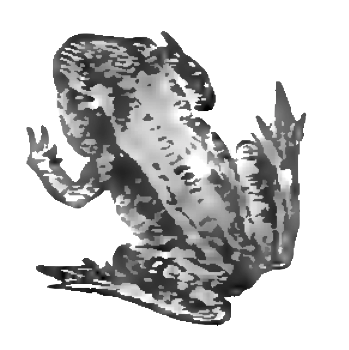
\includegraphics[width=0.5cm]{gfx/frog.png}} \Rightarrow v$). Then, the speaker model assigns a measure of goodness to the utterance predictions:
\begin{equation*}
\mathrm{Pr}(\mathrm{``there~is~a~frog"} | v) = f_{\Theta_s}([\mathrm{``there"},\mathrm{``is"},\mathrm{``a"},\mathrm{``frog"}], v)
\end{equation*}
\noindent In other words, the model of grounded meaning is also a model for connecting utterances to sensory evidence. 
The internal representations are not directly connected to external references. 
They are interpretations of the sensory readings internal to the agent. 
The mapping function between visual sensory inputs and internal agent representations could be modelled with a pre-trained convolutional network enriched with other contextual information about the situation. %
The model establishes uncertain links between primitive sensory readings and utterances of natural language, for that reason it functions as a model of grounding. 
In section~\ref{sec:concepts:convnets}, we describe some properties of this representation space and how sensory features would be mapped onto this representation space.




\section{Modelling compositionality}
\label{sec:concepts:compositionality}
One of the challenges of a model of grounding is formulated as Harnad’s symbol grounding problem \citep{harnad1990symbol}. 
The argument is that the capacity of learning from limited data is problematic when it is expected to impose new links to potentially unlimited compositions in a symbolic representation system.
The challenge is to infer grounded meanings for new representations (e.g. \textsc{`zebra'}) from known bottom-up representations learned from images (e.g. \textsc{`horse'} and \textsc{`stripes'}) 
when a symbolic link between them (\textsc{`zebra'} and a composition of two others) is established in natural language (\textsc{`zebra'} = \textsc{`horse'} + \textsc{`stripes'}).
In other words, compositionality as an ability to construct new representations linked to both sensory and abstract linguistic representations creates a generalisation problem for bottom-up learning.
The underlying premise of Harnad’s formulation of the problem is that human language is symbolic;
therefore, when human behaviour shows the capability of learning from language input, the establishment of such links came from new symbolic rules imposed by new statements of the natural language.

Without this explicit premise about the nature of language, the recent literature of language modelling stretches the notion of compositionality. 
In one account, any function in a semantic vector space is a model of compositionality \citep{mitchell2010composition}. 
In another direction, the semantic parse trees of linguistic expressions are used for composing neural network modules \citep{andreas2016neural}.

The notion of compositionality in natural language that we use in this thesis is simply the extent of generalisation in bottom-up training. 
The grounding of known representations is the learned link between natural language utterances and their internal neural representations.
The representation space imposes the compositional and structural links (\textsc{`zebra'} = \textsc{`horse'} + \textsc{`stripes'}), which are either learnable without intrinsic structures in space from data or learnable with extended structural or top-down control or design of the intrinsic properties’ representation units.



\section{Generative language model}
\label{sec:concepts:glm}
When the target of predictions in Equation~\ref{eq:probabilistic_model} is a linguistic unit, the model is what we call a \emph{probabilistic language model} \textemdash predicting the next word given previous sequences of words.
\begin{equation}\label{ch3:eq:lm0}
\mathrm{Pr}( w_{t+1} | w_{1:t} ) = f_{\Theta}(w_{t+1}, w_{1:t})
\end{equation}
\noindent where $w_{1:t}$ represents the given sequence of words at time step $t$ and the random variable is the target token at time $t+1$, here represented with a shorthand annotation for the probability of $w_{t+1}$. The sampling process from this model can potentially be part of a model designed to generate sequences of any length:
\begin{equation}\label{ch3:eq:lm}
\mathrm{Pr}( w_{1:T} ) = \prod_{t=1}^{T-1} \mathrm{Pr}( w_{t+1} | w_{1:t} )
\end{equation}
\noindent when coupled with a search algorithm, such as beam search, can be used for language generation. When the model function is based on recurrent neural networks, we call it a \emph{recurrent generative language model}, shortened to a \emph{recurrent language model}:
\begin{align}
\mathrm{Pr}( w_{t+1} | w_{1:t} ) &= f_{\Theta}(w_{t+1}, h_t) \\
h_t &= \mathtt{rnn}_{\theta_1}(h_{t-1}, w_t) \\
f_{\Theta}(w_{t+1}, h_t) &= \mathtt{softmax}(g_{\theta_2}(h_t))[w_{t+1}]
\end{align}
\noindent where $h_t$ represents the recurrent state at time $t$. 
This could also be interpreted as an agent representation in Equation~\ref{ch3:eq:utt} for generating each token. 
Two important modules of the language model are  $\mathtt{rnn}_{\theta_1}$, the recurrent module, and $g$, the top module, often a multi-layer perceptron, the output of which is a vector with the size of the vocabulary. In the end, $\mathtt{softmax}$ is the final activation function over all possible tokens in the vocabulary:
\begin{equation}
\mathtt{softmax}(V) = [\frac{e^{x}}{\sum\limits_{x' \in V}{e^{x'}}}]_{x \in V}
\end{equation}
\noindent where $V$ represents a vector of vocabulary size. After activation with $\mathtt{softmax}$, the output resembles a categorical probability distribution of the vocabulary.
The notation $\mathtt{softmax}(\cdot)[w]$ represents the predicted probability for $w$ at the output vector.
The unfolded representation of the model function would be as follows:
\begin{equation*}
\mathrm{Pr}( w_{t+1} | w_{1:t} ) = f_{\Theta}(w_{t+1}, \mathtt{rnn}_{\theta_1}(\mathtt{rnn}_{\theta_1}(...\mathtt{rnn}_{\theta_1}(h_0,w_{1})..., w_{t-1}), w_t))
\end{equation*}
The parameter set of the model, $\Theta$, is comprised of two partitions, ${\theta_1, \theta_2}$, from the two main modules of the model. 
The most common recurrent neural network we will use in this thesis is long-short term memory (LSTM) \citep{hochreiter1997long}.
We often add a trainable embedding layer in addition to the recurrent neural network to learn token representations. 
When a generated utterance is supposed to describe the content of an image or other situation, the generative language model in Equation~\ref{ch3:eq:lm0} and \ref{ch3:eq:lm} could be written as a conditional probability similar to the speaker model in Equation~\ref{ch3:eq:utt}: 
\begin{align}
\mathrm{Pr}( w_{t+1} | w_{1:t}, c ) &= f_{\Theta}(w_{t+1}, h_t, c) \label{ch3:eq:token_model}\\
\mathrm{Pr}( w_{1:T} | c)           &= \prod_{t=1}^{T-1} \mathrm{Pr}( w_{t+1} | w_{1:t}, c )
\end{align}
\noindent where $c$ represents the encoding of the situation \textemdash  visual features and the fusion of two representations, $h_t$. $c$ is the agent’s grounded representation in the speaker model in  Equation~\ref{ch3:eq:utt}. 

In these models, the uncertainty measures of the language model could also be interpreted as the degree of acceptability of linguistic units. 
With the speaker rationality assumption, the distribution of utterances in training data should not be very different from the acceptability judgment rankings. 
The generative language model learned from this data is also a model of acceptability judgments. If the language model can accurately predict acceptability judgments, it can be considered a model of syntax. 
It has been argued that such a language model is also an implementation of syntax without underlying categorical syntactic rules \citep[Section~3]{lau2017grammaticality}.

On the other hand, predicting the categorical distribution of tokens in their positions is, in fact, a model for the substitutability of words (i.e. Equation~\ref{ch3:eq:token_model}). 
Such a model loosely simulates substitutability of tokens.
Therefore, the vector representations learned for tokens and words in these models loosely posses the attributes for lexical-semantic representations.
This notion of meaning representation is consistent with the grounded representation discussed in section~\ref{sec:concepts:grounding}.
Based on these two arguments, a neural language model must be able to encode knowledge about syntax and semantics in the form of the neural network modules’ structure and parameterised representations. 
To predict the model outputs, parameters such as embeddings and intermediate representations of modules (contextualised embeddings) encode relevant knowledge learned from the training data.


\section{Modelling convolutional neural networks}\label{sec:concepts:convnets}
In section~\ref{sec:concepts:grounding}, we mentioned the possibility of using a function such as convolutional networks to map visual inputs onto a representation space for language grounding.
Here we discuss two aspects of using convolutional neural networks as a feature extraction function:
\begin{itemize}
	\item[(1)] How do convolutional neural networks process images?%
	\item[(2)] What types of knowledge are encoded in convolutional representations?
\end{itemize}

The role of convolutional networks (ConvNets) as a mapping function is to take basic two-dimensional pixel representation of images from a colour feature space, then project it onto another feature space that can discriminate images based on their content.
The most basic form of visual understanding is to recognise objects and entities in images.
A set of features that can distinguish visual differences between objects would be enough for most tasks.
For this reason, the most common way to use ConvNets in a variety of visual processing tasks is to train it as a module in an object recognition model, then use it as feature extraction module in other tasks and models.
The success of ConvNets in an object recognition task \citep{krizhevsky2012imagenet} with a large ImageNet dataset  \citep{deng2009imagenet} was the landmark deep learning success in computer vision. 

Conceptually, an object recognition model has the following modular design:
\begin{align}
\mathrm{Pr}( category | I ) &= f_\Theta(category,I) \\
\mathbb{V}_{I}              &= \mathtt{ConvNet}_{\theta_1}(I) \\
f_\Theta(category,I)        &= \mathtt{softmax}(\mathtt{mlp}_{\theta_2}(\mathtt{flatten}(\mathbb{V}_{I})))[category]
\end{align}
\noindent where $f$ is the uncertainty model for recognising a category of the object given the image $I$. 
The model has two modules \textemdash $\mathtt{ConvNet}_{\theta_1}$, the convolutional network for feature extraction and $\mathtt{mlp}_{\theta_2}$, the multi-layer perceptron for classification based on convoluted features. The most important property of ConvNets is that it can transfer object recognition knowledge to find patterns of local structures \citep{lecun2010convolutional}.

For recognising objects, we need a feature representation that would be, to some extent, invariant to spatial transformations. Geometric transformations such as shifting, rotating and rescaling have limited effects on recognising an object. Notable image representations such as the scale-invariant feature transform (SIFT) \citep{lowe2004distinctive} and the histogram of oriented gradients (HOG) \citep{dalal2005histograms} were motivated by this requirement. 
However, object recognition is not strictly invariant to geometric transformations. Spatial compositions at a global level can change the interpretation of smaller patterns. 
For these reasons, ConvNets was designed with the prior knowledge that identifying local patterns in different scales is essential. 
Then, for all possible regions of the image, as pre-defined granularities, their receptive fields would be mapped onto a new feature space. 
The feature mapper (or the kernel function)
with input as small as 3x3 pixels interprets local regions into a new representation space.
The term \emph{convolutional network} refers to multiple stages of feature mapping followed by spatial sub-sampling, which finally produces a representation with a coarser space but richer representations. 
After stacking the modules of feature mapping with sub-sampling, each broader region is mapped to a vector representation.

Although prior knowledge about the task led to its design and the popularity of ConvNets in several tasks, there is limited theoretical understanding about how and what geometric features are encoded in convoluted representations.
Based on one account, these features are useful for localisation and object detection tasks, without an algorithmic search \citep{Lenc15a,ren2015faster}. 
In another account, the recognition tasks are sensitive to local geometric transformations\footnote{The recognition of a face depends on the spatial relationships between eyes and nose \citep{hinton2011transforming}}
and ConvNets relax the geometric knowledge; therefore, geometric relationships between local parts in lower layers decay when reaching the higher layers \citep{hinton2011transforming,lenc2015understanding,kelleher2017what}. 

Based on these two accounts:
\begin{itemize}
	\item[(1)] The geometric features in convolutional representations are a continuum of relational features among smaller regions and larger super-pixels;
	\item[(2)] These are locally relaxed at the final layers to the extent that convolutional representation may have lost its geometric knowledge.
	This is an important consideration when we want to ground spatial relations in natural language on these visual representations.
\end{itemize}

\section{Conclusion}
\label{sec:concepts:conclusion}

We explained that any modelling requires a set of assumptions; modelling with neural networks encodes these assumptions into the model architecture, training datasets and objectives. 
We addressed the neural network modelling for grounded representations, compositionality and language generation. 
All these models correspond to challenges in meaning representations. 
In the next chapter, we summarise our studies on spatial knowledge encoded in the language models.
\chapter{Summary Of Studies}
\label{sec:related}



In this chapter, we summarise the questions, methods and findings of six studies and discuss their relevance to the main aims of the thesis.

\section{Study 1: Functional/geometric bias in neural language models}
\label{study:fungeo}
Simon Dobnik, Mehdi Ghanimifard, and John Kelleher. 
Exploring the Functional and Geometric Bias of Spatial Relations Using Neural Language Models.
\textit{In Proceedings of the First International Workshop on Spatial Language Understanding, pp. 1-11. 2018.}

Understanding spatial language is fundamental to human-robot interactions. 
The meaning of spatial relations in scene descriptions is grounded in the geometry of the scene and the functional relationship between objects. 
We used a neural language model on a large corpus of image descriptions to investigate the earlier observations about functional bias in spatial relationships.
We contributed to understanding that are encoded in unimodal neural language models.

\subsection{Questions}

Does the performance of trained neural language models on relational descriptions in the Visual Genome dataset  \citep{krishna2017visual} account for the expectation that more functional spatial relations are more predictable based on the objects they describe? 

We propose two hypotheses: 
\begin{itemize}
	\item Descriptions with functional relations (in contrast with geometric relationships) have lower perplexity in their language model over the held-out test suite (more likely gold-standard descriptions) because they describe a functionally common situation. The target/landmark object pairs in the dataset are more specific to functional relations compared to geometric relations. 
	\item When modifying spatial relations with any alternatives, the phrases with the initial choice of functional relations gain increased perplexity because they are more contextually dependent on targets and landmarks compared to geometric relations.
\end{itemize}


\subsection{Method}
We trained the neural language model on image descriptions in Visual Genome. Then, we measured the perplexity of the model on held-out descriptions based on their spatial relations. In our experiments, we examined the hypothesis on both natural occurring descriptions in the dataset and the down-sampled balanced dataset.

\subsection{Findings and conclusions}
We observed from the perplexity of the language model that functionally-biased spatial relationships are more predictable when the model was trained on the dataset with a naturally occurring frequency of descriptions.
However, training the model on a down-sampled dataset did not result in the expected outcome of perplexities for each test group.%
We reported a more detailed examination of sensitivity %
of the language model.
Our observation showed that the degree of sensitivity for target and landmark is not the same in the two groups of spatial relations. 
A possible explanation for different sensitivity for targets and landmarks is the misalignment between word order, semantic structure of relations and the cognitive process of choosing related objects as landmark and target. 
Misalignment of word order and the underlying semantic structure of spatial expressions explains why the forward and backward direction language models have different levels of perplexity.

The second category of the hypothesis was only partially confirmed. 
Only a few spatial relations confirmed the hypothesis. 
While some geometric relations, such as \emph{`above'} tend to see a high degree of change in perplexity when replaced with other spatial relations, the dependency of geometric relations on the textual context leaves interesting open questions about the world knowledge and spatial knowledge in neural language models.

\paragraph{Author contributions}
Mehdi Ghanimifard had the main responsibility for implementing the model, conducting the experiments and reporting it. Simon Dobnik and John Kelleher had shared responsibility for the remaining aspects of this research. All authors read and approved the final manuscript.

\section{Study 2: Representation of spatial relations in neural language models}
\label{study:what}
Mehdi Ghanimifard and Simon Dobnik. 
\emph{What} a neural language model tells us about spatial relations.
\textit{In Proceedings of the Combined Workshop on Spatial Language Understanding (SpLU) and Grounded Communication for Robotics (RoboNLP), pp. 71-81. 2019.}

We followed up the question about possible encoded knowledge in section~\ref{study:fungeo} about spatial relations in unimodal neural language models.
In this work, we extend the method to inspect the knowledge of spatial relations in generative language models. 
One of the methods for measuring lexical knowledge in distributional semantics is analogical reasoning tasks. 
The knowledge of spatial relations in the image description task may be different from the visual-cognitive knowledge required for human judgment on spatial relations, so we also examined if learned representations are transferable to other tasks.


\subsection{Questions}
\begin{itemize}
	\item What should we expect from a contextualised model of spatial relations based on textual features in terms of their functional and geometric bias?
	\item How can we inspect these in a generative language model? 
	\item How do the learned representations from the generative model compare with representations from human judgments?
\end{itemize}

\subsection{Method}

We trained a generative LSTM language model on region descriptions. 
Then, we inspected %
how the language model encodes descriptions of spatial relations in swapped contexts of target and landmark objects in terms of perplexity.
We proposed a method in which word-context vectors are produced based on augmented datasets, swapping spatial relations in the context of other spatial relations. Perplexities of these generated word-context examples built perplexity-based vector space for spatial relations. 

We ran analogical tests on these vectors and other textual embeddings to inspect how these representations differed from each other. 
Finally, we compared them with vector representations of human acceptability judgments and relatedness judgments.

\subsection{Findings and Conclusions}
In the absence of the image, we expected contextual representations to learn object-specific knowledge (functional knowledge). 
However, the learned representations showed high performance in solving analogical tasks that required also some sense of geometry. 
Our analysis is that functional knowledge must be complementary to geometric knowledge, which is why language models can partly solve these puzzles. 
These finding were also confirmed with qualitative inspections,
for example
the representations of \emph{`left'} and \emph{`right'} were similar to each other and different from \emph{`above'} and \emph{`over'}.

The task of judging acceptabilities, the task of generating descriptions and annotations, and the task of finding related words are three different tasks, perhaps using different kinds of spatial knowledge.
The last experiment comparing the similarities of representations in the image description task, acceptability judgments and relatedness experiments hinted that spatial relations in the image description task might use different types of knowledge about space and spatial relations. 

The findings of this study raise questions that links this study to study four and five.
Knowing that textual context provides discriminative features for identifying spatial relations, we argue that, in language generation tasks, one can ground the word choices in textual evidence. 
Generative neural language models can encode task-specific knowledge of space, including functional and geometric bias, when describing the relation between two objects. 
With this insight, the consequence of memorised knowledge is an open question for multimodal language models \textemdash how does a multimodal language model balance the attention to knowledge of the scene and linguistic representations in the task? 

\paragraph{Author contributions}
Mehdi Ghanimifard had the main responsibility for implementing the model, conducting the experiments and reporting it. Mehdi Ghanimifard and Simon Dobnik had shared responsibility for the remaining aspects of this research. Both authors read and approved the final manuscript.

\section{Study 3: Functional/geometric spectrum in bounding boxes}
\label{study:bbox_grounding}
Simon Dobnik and Mehdi Ghanimifard. 
Spatial descriptions on a functional-geometric spectrum: the location of objects.
\textit{Preprint - 2020.}

In the previous two studies, we investigated the distributional properties of spatial relations in language. 
We argued that functional knowledge and geometric knowledge are encoded in distributional representation, which can be captured to some extent with neural language models. 
To complement this study on the grounding of spatial relations for image descriptions, we extended the investigation on the distributional properties of bounding boxes for the spatial relations that describe them. 
More specifically, in this study, we used bounding boxes to extract the basic geometric features of the relations between two objects. 
Then, we inspected the geometric feature distribution of each %
spatial relation.

\subsection{Questions}
\begin{itemize}
	\item Are the bounding box features extracted from annotated images reliable descriptors for spatial relations; do the extracted features correspond to other geometric representations, such as spatial templates? 
	\item Are geometrically biased spatial relations%
	obtained in constrained experimental settings
	reflected in more predictable locations of objects?
	Can they be mapped into fewer variations of their related object locations?
\end{itemize}

\subsection{Methods}
For each relation, we collected the pairs of bounding boxes from the relationship dataset in the Visual Genome \citep{krishna2017visual}. 
After standardising the bounding boxes, each pair of objects produced several feature vectors $[x, y, d]$.  Inspired by the Attentional Vector Sum (AVS) model  \cite{RegierCarlson:2001},
the bounded boxes were converted to feature vectors that expressed the geometric relations between individual locations of objects.
The expected feature vectors for each spatial relation 
are
comparable with %
spatial templates. 
Then, we inspected the variations and skewness of the feature vector distributions from their centroid to determine if this%
accounts for geometric bias.  
The lower the variation, the more geometrically biased is the relation.

\subsection{Findings and conclusion}
We found that the bounding box features %
represented as the
weighted sum vectors from acceptability scores in spatial templates for projective relations. 
We found that the feature vectors for geometrically biased relations diverge less from the average vectors compared to their more functionally biased equivalent relations. 
The distribution of feature vector divergence from the average vector is more skewed toward zero when they describe a geometrical relation. 
We also inspected the properties of some verbal relations with spatial content. 
These spatial features indicate spatial regularities in the image description dataset.
Practically, the findings of this study would be helpful when designing models for image captioning, as it demonstrates the representations that are relevant for different types of descriptions.

\paragraph{Author contributions}
Mehdi Ghanimifard had the main responsibility for implementing the model, conducting the experiments and reporting it. Simon Dobnik and Mehdi Ghanimifard had shared responsibility for the remaining aspects of this research. Both authors read and approved the final manuscript.

\section{Study 4: Evaluating generation of spatial descriptions with adaptive attention}
\label{study:knowing}
Mehdi Ghanimifard and Simon Dobnik. 
Knowing When to Look for What and Where: Evaluating Generation of Spatial Descriptions with Adaptive Attention.
\textit{The European Conference on Computer Vision (ECCV) Workshops, pp. 153-161. Springer, Cham, 2018.}

The neural network model in \citep{lu2017knowing} provides an attention mechanism that expands the domain of attention from spatial attention on visual features to hidden states in the language model. 
In sections~\ref{study:fungeo}~and~\ref{study:what} we explored the possibility of memorising specific spatial knowledge in a unimodal language model, including functional and task-specific spatial relations between objects. 
In this study, we wanted to determine how a multimodal language model uses it in a language generation task. 
The attention on linguistic features when knowledge from different sources generating different parts of speech and,
more specifically, on spatial relations can explain the grounding of the generation model in multimodal information, including the contextual representations in the language model memory. 

\subsection{Questions}
\begin{itemize}
	\item How does the attention on visual features and linguistic features change for different parts of speech?
	\item Is there any difference in the magnitude of attention on visual features between targets and in landmarks?
	\item Are spatial relations grounded in visual features? %
\end{itemize}

\subsection{Method}
The adaptive attention between visual features and linguistic features compete with each other. 
The magnitude of attention on linguistic features is a sign of dependence on language and context instead of a grounding in visual features.
In this study, we inspected adaptive attention as a source of explanation for grounding. 
The average of attention on linguistic features for each part of speech and, for each semantic role in spatial descriptions (target, relation, landmark) is interpreted as an indication for a lack of visual grounding.
We compared the 
ranking
of attentions with the rankings of accuracy rates of a uni-modal language model predicting a mismatch, whether a part of speech has been replaced in the FOIL captions \citep{shekhar2017vision}. %
We also qualitatively examine the average spatial attentions of descriptions containing each spatial relation; the spatial attention on target, landmark and spatial relation.

\subsection{Findings and conclusion}

The degree of attention on linguistic features varies depending on the part of speech. In particular, we found that the attention on visual features drops when predicting spatial relations compared to the average attention on noun phrases. 
The average visual attention on parts of speech partially reflected the results from the FOIL task. For example, nouns are highly visually attended but difficult to predict by the language model, the adpositions (prepositions and postpositions) were ranked among the least visually attended parts of speeach while there were moderately predicatable in the FOIL task.

There are three possible explanations for these results:%

\begin{itemize}
	\item[(1)] Spatial relations are more functional and object dependent in these tasks. Therefore, object-specific spatial features (spatial affordances of objects) encoded in language models are more likely to be predictive of spatial relations than visual clues in the image.
	\item[(2)] CNNs do not have 
	represent geometric
	locational information required for grounding spatial relations. As they are trained for object identification, there is some degree of spatial invariance in these features.
	\item[(3)] Using softmax for modelling attention is a 
	disadvantage 
	in cases where spatial attention is distributed over several objects and their relation.
	Spatial relations depend on target, landmark and locational features; therefore, the softmax model of attention is noisier when it attends to multiple locations for predicting spatial relations.
\end{itemize}


\paragraph{Author contributions}
Mehdi Ghanimifard had the main responsibility for implementing the model, conducting the experiments and reporting it. Mehdi Ghanimifard and Simon Dobnik had shared responsibility for the remaining aspects of this research. Both authors read and approved the final manuscript.

\section{Study 5: Generating descriptions with top-down spatial knowledge}
Mehdi Ghanimifard, and Simon Dobnik. 
What Goes Into A Word: Generating Image Descriptions With Top-Down Spatial Knowledge.
\textit{In Proceedings of the 12th International Conference on Natural Language Generation. 2019.}


As we continued to question how the neural language model learns spatial knowledge, we investigated the effects of top-down knowledge on space in generating relational image descriptions. As seen in section~\ref{study:knowing}, the attention mechanism for the generative recurrent language model can control and explain how different modalities contribute to generation tasks. In this study, we integrated 
specific geometric and non-geometric features that are considered relevant in top-down computational models
of spatial descriptions into the design of the attention model. We compared the effects of three types of top-down spatial knowledge: 
\begin{itemize}
	\item[(1)] Where objects are obtained with a separate localisation procedure;
	\item[(2)] Which object is the target, and which is the landmark, with prior role assignment;
	\item[(3)] How they are geometrically related in images by representing their spatial configuration.
\end{itemize} 

\subsection{Questions}
\begin{itemize}
	\item[(1)] Which types of top-down spatial knowledge improve language generation? 
	\item[(2)] How does each category of features contribute to generating image descriptions?
\end{itemize}

\subsection{Method}
We experimented on a relationships dataset from the Visual Genome  \cite{krishna2017visual}, training several comparable neural network designs with different spatial modules 
and different types of top-down knowledge about spatial relations. 
We changed the attention module in these models 
to be able to attend over language model features, visual features and geometric features
and enriched the %
input representations with 
the additional geometric features representing the spatial configurations of objects.
In addition to comparing the performance loss on unseen examples, we inspected the attention module to determine what features had a dominant effect on generating descriptions.

\subsection{Findings and conclusions}
We observed that the overall performance improved with the additional top-down knowledge of space. 
However, the results showed a substantial contribution of the %
language model representations in generating descriptions. 
Among added spatial knowledge localisation had the strongest effect, while the effects of role assignment and geometric spatial features were mixed. 
The reasons behind this outcome may be the bias in two kinds of regularities in data \textemdash the spatial composition of objects in photos in this dataset (location of objects are meaningful from the perspective of the photographer) and the task of describing object relations may have neglected the application of certain geometric relations (\emph{`to the left of'}, \emph{`to the right of'})
but preferring general, less specific spatial relations such as \emph{`close'} and \emph{`with'}.

\paragraph{Author contributions}
Mehdi Ghanimifard had the main responsibility for implementing the model, conducting the experiments and reporting it. Mehdi Ghanimifard and Simon Dobnik had shared responsibility for the remaining aspects of this research. Both authors read and approved the final manuscript.

\section{Study 6: Learning to compose grounded spatial relations}
Mehdi Ghanimifard and Simon Dobnik. 
Learning to Compose Spatial Relations with Grounded Neural Language Models.
\textit{In IWCS 2017-12th International Conference on Computational Semantics-Long papers. 2017.}


A basic definition of grounding linguistic units in visual perception is to associate words and phrases with visual features. 
Learning these associations must generalise from limited examples to 
novel
unseen compositions.
Compositionality in language imposes a systematic generalisation to the grounding of words and phrases. 
Due to the broad application of recurrent neural language models in vision and language tasks, this study investigated the capability of a recurrent language model in learning these compositional generalisations in the grounded language.

\subsection{Questions}

\begin{itemize}
	\item To what extent is the language model trained on single examples can retrieve acceptability representations about the scene? 
	\item Is the recurrent language model capable of generalising from word compositions to phrase compositions and how does it perform over previously unseen word compositions?
\end{itemize}

\subsection{Method}
Simple spatial relations are composable and can be used to construct new relations, such as \emph{`above and to the right of'}, which denotes a relation constructed from two simple relations \emph{`above'} and \emph{`to the right of'}. We constructed artificially composed spatial templates based on their acceptability scores
of the individual
the spatial templates \citep{logan1996computational} using known compositional operations. 
Then, from these templates we generated synthetic 
examples of individual situations and descriptions based on the aggregated acceptability scores.
We tested different learning scenarios by controlling for unseen descriptions. 
In each experiment, we reconstructed the spatial templates of unseen descriptions based on the model scores over
the unfolded predictions of words.
Qualitatively, we measured the mismatches between the reconstructed templates and 
templates that were used to generate the artificial training data.

\subsection{Findings and conclusions}
We found that a grounded neural recurrent language model is capable of generalising when composing and decomposing word sequences both across the language and the perceptual domain.. 
We investigated the effects of three factors on the success of the task and found that the degree to which the training data was impoverished had the most substantial effect, the type of composition is an essential factor in learning compositionality, and the presence of ungrounded distractor words had a small effect.

These observations leave an open question \textemdash is the performance for certain compositions reliant on intrinsic structures of recurrent neural networks for learning specific functions or the frequency and variation of data due to the semantic and combinatorial properties of compositions? 
Negation has fewer possible variations compared to \textsc{`or'} phrases and \textsc{`and'} phrases; 
therefore, it produces fewer instances and fewer variations in the training data for the negation marker. 
Distribution of the training data affects the final learned embeddings for the tokens of \textsc{`and'}, \textsc{`or'} and \textsc{`not'}. 
Learning to encode negation as a function in the recurrent unit might be harder than encoding other functions. 

In summary, the combinatorial properties and semantics of different compositions affect the frequency and distribution of all tokens in language. 
While the distributional effects have potentially challenging consequences for the uniform learning of compositions, it can signal the difference between them.
This is why, despite the imbalance in the number of compositions, the model could learn not ground distractor tokens.%

\paragraph{Author contributions}
Mehdi Ghanimifard had the main responsibility for implementing the model, conducting the experiments and reporting it. Mehdi Ghanimifard and Simon Dobnik had shared responsibility for the remaining aspects of this research. Both authors read and approved the final manuscript.

\section{Study 7: Metaphoricity of compositions with distributional representations}
Yuri Bizzoni, Stergios Chatzikyriakidis and Mehdi Ghanimifard. 
``Deep'' Learning: Detecting Metaphoricity in Adjective-Noun Pairs.
\textit{In Proceedings of the Workshop on Stylistic Variation, pp. 43-52. 2017.}

Recognising metaphoric use of language requires an understanding of the situation, context and how expressions refer to extra-linguistic knowledge about the world. 
On the other hand, distributional knowledge in unimodal language models encodes word-context associations. 
Even without the presence of extra-linguistic knowledge of situations, distributional knowledge might be able to determine metaphorical adjective-nouns. 
In this study, we proposed that knowledge of the compositionality of adjective-nouns is encoded in the pre-trained word embeddings of textual corpora and a simple neural network can transfer this knowledge to metaphor recognition tasks. 
We used methods of vector composition in a neural network design to predict the metaphoricity of adjective-noun compositions.


\subsection{Questions}

\begin{itemize}
	\item Is it possible to detect metaphoric adjective-noun compositions using pre-trained word embeddings in a shallow neural network? 
	\item Are there any differences in performance between design choices and language model types, including word2vec \citep{mikolov2013distributed}, GloVe \citep{pennington-etal-2014-glove}, and dependency-based embeddings \citep{levy-goldberg-2014-dependency}?
\end{itemize}

\subsection{Method}
We compared different methods of vector composition in a neural network design, similar to \cite{mitchell2010composition}, and used different pre-trained word embeddings. 
We examined the performance of these models with cross-validation on unseen adjectives and unseen adjective-noun pairs.

\subsection{Findings and Conclusions}
We found that pre-trained word embeddings with simple neural network designs performed better than previous approaches without using word embeddings. 
This study raises a question if similar designs could expand metaphoricity judgments to other part-of-speech compositions. 
The high performance of the textual word embeddings up to 93\% accuracy confirms that unimodal language models can encode some knowledge of the referential meaning to real situations. 
However, questions concerning the type of knowledge and it are left for subsequent studies.

\paragraph{Author contributions}
Mehdi Ghanimifard had the main responsibility for writing the model section of the manuscript. Mehdi Ghanimifard and Yuri Bizzoni had shared responsibility on running the experiments and reporting it. Yuri Bizzoni and Stergios Chatzikyriakidis had shared responsibility for the remaining aspects of this research. All authors read and approved the final manuscript.

\section{Summary}
\label{sec:summaries:conclusion}

In the first three studies, we focused on latent extra-linguistic knowledge of spatial relations in unimodal neural recurrent language models and on geometric features as represented by bounding boxes. 

In studies 4 and 5, we examined the contribution of visual features, geometric features, and the contextual embeddings of a neural language model when generating image descriptions. 
We showed that, in training generative neural language models, the spatial knowledge used in the task is also learned latently in language models. 

In the last two studies, the focus of the research was on the capability of neural language models to learn compositional knowledge and generalise from limited samples to new word compositions.

\chapter{Final Discussions}
\label{sec:conclusion}


\section{From aims to findings}
This thesis aimed to build and examine systems capable of generating and understanding situated language. 
Using deep neural networks, we may be able to build language models to imitate natural language. 
However, explanations are required regarding what knowledge is encoded in the models, how the models encode relevant knowledge and if such data-driven methods satisfy the systematic generalisations required for going beyond limited data sets. 
The recent success of deep learning methods in vision and language tasks are promising and challenge theoretical discussions about language grounding and explainability. 

A study on spatial expressions in image descriptions provides challenges and broad applications of a vision and language model for situated language processing. 
The challenge is to understand how a model should and would ground language in spatial knowledge. 
Spatial knowledge could include the geometry of a scene and the location of objects; 
alternatively, it could include causality in physics and the functional affordance of objects in relation to each other. 
The grounding of linguistic categories in these two types of knowledge presents a challenge for disentangling the representation of two types of knowledge. 
In the context of deep learning methods, we asked three research questions:
\begin{itemize}
	\item[(Q1)] What type of spatial knowledge is encoded in language models?
	\item[(Q2)] How does the model encode semantic knowledge?
	\item[(Q3)] Is there systematic generalisation of the knowledge?
\end{itemize}

In seven studies, we %
contributed
to the discussion on grounding and 
answered the
questions regarding the use of neural language models. The first \citep{dobnik-etal-2018-exploring} and the second \citep{ghanimifard-dobnik-2019-neural} studies focused on unimodal language models for spatial descriptions. The corpus data suggests a statistical dependency between semantic components of a spatial description $\langle\textsc{Target}$, $\textsc{Relation}$, $\textsc{Landmark}\rangle$.
This %
explained with the functional meaning of spatial relations. 
The fact that %
spatial descriptions of object pairs are predictable is mostly because of their functional relationship. 
The overlap between the functional and geometric sense in linguistic categories of spatial relations %
contributes to the encoding of knowledge about geometry in word distributions as well. 
On the other hand, both
studies suggest the possibility that, in an image description task, spatial expressions tend to explain \emph{what} the objects are in the picture instead of \emph{where} they are. 
Therefore, the non-geometric sense of spatial descriptions has a strong
effect in these corpora. 

With a 
focus on
spatial grounding in the spectrum of functional/geometric sense of relations, in our third study, we looked at the geometric properties of bounding box annotations in images and their distributions 
for different
spatial expressions. 
We found that the variation in the relative location of objects in geometrically biased expressions is lower than 
in the functionally biased relations.
This finding is consistent with the predictability of functional relations from linguistic evidence 
rather than geometric 
features.
This conclusion has implications for the evaluation of multi-modal language models, which brought us to the fourth and the fifth studies.

The fourth study \citep{ghanimifard2018knowing} examined the possibility of evaluating grounding based on adaptive attention. We found that pre-trained convolutional visual features contributed more to the generation of nouns compared to other parts of speech. Some spatial relations are more dependent on contextual language embeddings. This is consistent with our view that spatial relations in image descriptions are less dependent on the 
location of objects. 
Due to the opaque representation of space in convolutional features,
further studies are required how these contribute to spatial expressions and whether such representations can be improved with feature engineering.
 

In the fifth study \citep{ghanimifard-dobnik-2019-what}, we extended the adaptive attention to 
enrich
the visual features with locational information. We found that top-down algorithmic localisation has the most positive effect on language generation among the different methods for enriching visual features. 
The effect of both a top-down semantic role assignment and geometric feature vectors is positive, but 
much less than expected.
This observation is consistent with our findings in the third and fourth studies on unimodal language models, which indicated that reliable predictability of object relations without visual features varies depending on the kind of spatial relations in the absence of adequate geometric descriptions. 
These observations demand 
further 
studies, especially beyond image description tasks, for example in visual question answering.

In the sixth study \citep{ghanimifard-dobnik-2017-learning}, we%
examined
the degree of generalisation%
a recurrent language model learned compositional descriptions. 
We found that the generalisation depends on both the combinatorial and semantic properties of the compositions. 
The combinatorial properties of compositions change the variations and frequencies of possible phrases (unary vs binary compositions). 
The semantics of the compositions shape the acceptable space. 
, for example conjunction and disjunction result in different frequencies.
Both combinatorial and semantic properties of compositions contribute to token distributions in language.

In the seventh study \citep{bizzoni-etal-2017-deep}, we examined if the knowledge from a unimodal language model could recognise the metaphoricity of adjective-noun compositions.
This contributed to an understanding of the type of knowledge that could be encoded in the language model. 
Distribution of tokens, as seen in the first study, could affect the generalisation in language grounding. According to this study, it 
contributes to encoding of deeper
non-perceptible knowledge, such as metaphors.


\section{Knowledge and grounding}
One of the central claims of this thesis is that some spatial knowledge is encoded in neural language models. Then, despite the fact that representations in language are not linked to primitive sensory representations, we used the term \emph{grounding} for spatial descriptions that are explainable with a language model instead of perceptual inputs.
This argument requires a more in-depth discussion about the definition of \emph{spatial knowledge} and \emph{grounding}.

\paragraph{Spatial knowledge}

In this thesis, the term knowledge was extensively used to
describe 
language grounding in (1) \emph{spatial knowledge}, (2) \emph{geometric knowledge}, (3) \emph{functional knowledge} and (4) \emph{distributional knowledge} or \emph{knowledge in language models}. 
The main argument of the thesis is that spatial language projects
onto the representations in language models. 
Therefore, distributional knowledge of spatial relations encodes the spatial knowledge (findings of studies 1, 2, 4 and 5 concerning Q1). 
Nevertheless, the distinction between functional and geometric knowledge implies that there are two different types of spatial expressions. 
Geometric knowledge is a literal sense of space and functional knowledge is an abstraction of non-spatial relations between objects. 
We expect that, by capturing regularity in language use, distributional knowledge captures functional knowledge (study 1 concerning Q1). 
However, the distributional distinction between functional and geometric use is entangled in datasets. 
Therefore, distributional knowledge captures regularities that seem more geometric than functional. 

This distributional property is an artefact of the entangled concept of space. The skewness of spatial relations in datasets is a result of this entanglement. 
For example, the reason the functional sense of the relation \emph{`over'} as a sheltering relation is possible is because of its geometric properties and the rules of physics. 
Similarly, the reason why some objects are functionally related is because of their geometric shapes and their geometric capacity of being in that position. 
The entangled relation between functional and geometric meaning calls for a better understanding of spatial knowledge. 
Without spatial reasoning, the functional meaning of the relations is not possible. 
In this, we argued that language models capture spatial knowledge, but 
also that there are different types of spatial knowledge and what their implications are for descriptions in different contexts.
The evaluation of the relation between the knowledge kinds in different contexts in which spatial descriptions are made should be addressed in future work.

\paragraph{Grounding}
The conclusion of this thesis with regard to grounding is that any prediction based on the available evidence is a form of grounding. 
The representation of this evidence varies in models. 
Predictions of a show-and-tell system are grounded in both situated features and the 
modelling assumptions, such as the function and design of the model (composition of modules), its training data %
(sufficient data for model convergence) 
and its learning goals.
Therefore, when %
the system makes 
predictions without relying on situated features or with minimal attention to these situated features, there are two explanations of this performance:
\begin{itemize}
	\item[(1)] Some assumptions used building the model are erroneous, such as the assumption around what training data provides sufficient knowledge for constructing the model.
	\item[(2)] The situated features do not contain independent encoding of knowledge required for the task. In other words, the task relies on other information, such as world knowledge. This kind of missing information could be included as different representations of the model. This can be done by:
	\begin{itemize}
	\item[(i)] a module
	that fuses
	language and vision
	to exploit the fusion of
	the situated features with other representations, or 
	\item[(ii)] exclusively encoding some knowledge about the task in modules, such as language models, that provide distributional evidence. 
	\end{itemize}
\end{itemize}

In the case of generating spatial descriptions, the predictability of relations from textual evidence or with minimal contribution from visual features has two explanations:
\begin{itemize}    
	\item[(1)] There might be mistakes in the model design, feature representations or the assumption that training data has appropriate information for the task. 
	For example, knowledge about embodied actions and interactions between objects may be missing from show-and-tell datasets.
	\item[(2)] Some spatial knowledge is encoded in the distributional knowledge of language, in addition to situated visual knowledge, such as functional knowledge and frame of reference. 
	The neural language model encodes this knowledge in its parameters. 
	The composition of the visual module and the language module contextualises the representations based on the training data. %
\end{itemize}

With this conclusion about grounding, we can examine the future improvements of vision and language models. 

\section{Future work}

The discussion 
of
grounding 
and
learning representations with deep learning methods opens several directions for future research:
\begin{itemize}
	\item The current model designs use simple tools of modality fusion, such as embedding representations, attention mechanisms and simple vector manipulations, including concatenation or multiplication. 
	More research on modality fusion is required in future studies.
	\item Our attempts to understand what is learned in neural language models can be expanded 
	with additional
	methods of explainability and probing representations. 
	The question of what representations are learned and what are the effect of parameters is beneficial for %
	improving
	the algorithms.
	\item In addition to investigating explainability and developing better modules, more rigorous testing of models is required to measure their success. Such a study would 
	lead to development of
	better learning goals and loss functions for the model. Instead of language modelling with token level loss, new loss functions related to task problem-solving, such as spatial navigation, may be able to learn different aspects of meaning in language models. 
	\item This requires a better understanding of the data. We found two types of bias in image description datasets:
	\begin{itemize}
		\item[(i)] The bias in the task constrains the words to specific senses. 
		In the image description task, spatial relations have a strong bias towards relating \emph{what} is in the picture, instead of relating \emph{where} objects are in respect to each other.
		\item[(ii)] The bias in the visual composition of images. The images in image captioning datasets are focused on objects in regions of interest. 
		This suggests that other datasets should also be examined, such as those collected from ego centric robotic sensory and imaging data, which lack such a focus of attention on objects as a property of image compositions.
	\end{itemize}
\end{itemize}


\bibliographystyle{acl_natbib}
\bibliography{references.bib}

\part{Studies}


\chapter{Functional/Geometric Bias In Neural Language Models}
\chaptersource{Simon Dobnik, Mehdi Ghanimifard and John Kelleher.}{Exploring the functional and geometric bias of spatial relations using neural language models,}{In Proceedings of the First International Workshop on Spatial Language Understanding, pp. 1-11. 2018.}

\paragraph{Abstract}
  The challenge for computational models of spatial descriptions for
  situated dialogue systems is the integration of information from
  different modalities. The semantics of spatial descriptions are
  grounded in at least two sources of information: (i) a
  geometric representation of space and (ii) the functional interaction
  of related objects that. We
  train several neural language models on descriptions of scenes from
  a dataset of image captions and examine
  whether the functional %
  or geometric %
  bias of spatial descriptions reported in the literature is reflected
  in the estimated perplexity of these models. The results of these experiments have implications for the creation of models of spatial lexical semantics for human-robot dialogue systems. Furthermore, they also provide an insight into the kinds of the semantic knowledge captured by neural
  language models trained on spatial descriptions, which has implications for image captioning systems.



\section{Introduction}\label{splu2018:sec:spatial-descriptions}

Spatial language understanding is fundamental requirement for human-robot interaction through dialogue. A natural task for a human to request a robot to fulfil is to retrieve or replace an object for them. Consequently, a particularly frequent form of spatial description within human-robot interaction is a \emph{locative expression}. A locative expression is a noun phrase that describes the location of one object (the \emph{target object}) relative to another object (the \emph{landmark}). The relative location of the target object is specified through a %
prepositional phrase:
\begin{center}
Bring~me~$\underbrace{\underbrace{the~big~red~book}_{Target}~\underbrace{on~\underbrace{the~table}_{Landmark}}_{\substack{Prepositional\\Phrase}}}_{Locative~Expression}$.
\end{center}
\noindent In order to understand these forms of spatial descriptions a robot must be equipped with computational models of the spatial semantics of prepositions that enable them to ground the semantics of the locative expression relative to the context of the situated dialogue.

A natural approach to developing these computational models is to define them in terms of scene \emph{geometry}. And, indeed, there is a tradition of research that follows this path, see for example \cite{logan/sadler:1996,KelleherCostello:2005,KelleherCostello:2009}. However, there is also a body of experimental and computational research that has highlighted that the semantics of spatial descriptions are dependent on several sources of information beyond scene geometry, including \emph{functional semantics} (which encompasses a range of factors such as world knowledge about the typical interactions between objects, and object affordances) \cite{Coventry:2004aa}. We can illustrate this distinction between geometric and functionally
defined semantics using a number of examples. To illustrate a geometric semantics: assuming a spatial meaning, anything
can be described as \emph{to left of} anything else so long the spatial configuration of the two objects is geometrically correct.
However, as \cite{CoventryEtAl:2001} has shown the spatial description \emph{the umbrella is over the man} is sensitive to the
 protective affordances of the umbrella to stop rain, and is appropriate in contexts where, the umbrella is not in a
geometrically prototypical position above the man, so long as the umbrella is protecting the man from the rain.

A further complication with regard to modelling the semantics of spatial descriptions is that experimental results indicate that the contribution of geometrical and
functional factors is not the same for every spatial relation \citep{Garrod:1999fk,CoventryEtAl:2001}.  This experimental work shows that there is
an interplay between function and geometry in the definition of spatial semantics
and therefore the spatial meaning of given spatial relation is neither fully functional nor fully geometric. Rather, spatial terms can be ordered on a spectrum
based on the sensitivity of their semantics to geometric or functional factors.

Given the distinction between geometric and functional
factors in shaping spatial semantics, a useful analysis that
would inform the design and creation of computational models of spatial
semantics is \emph{to identify the particular semantic bias
(geometric/functional) that each spatial term evinces}. However, such an analysis is difficult. Native speakers do not have strong intuitions about the bias of
prepositions and such bias had to be established experimentally
\cite{CoventryEtAl:2001,Garrod:1999fk} or through linguistic analysis
\cite[p.55]{herskovits1986language}.\footnote{The discussion of Herskovits
  focuses on interaction of objects conceptualised as geometric
  shapes, for example \emph{on:} contiguity with line or surface. The
  fact that the interacting objects can be conceptualised as different
  geometric shapes points and therefore related by a particular
  prepositions points to their functional nature as discussed here.}
Reviewing the literature on this experimental and analytic work reveals
that prepositions such as \emph{in}, \emph{on}, \emph{at}, \emph{over}, \emph{under}
have been identified as being functionally biased, whereas \emph{above}, \emph{below}, \emph{left of} and \emph{right of} are geometrically biased. Other spatial
relations may be somewhere in between. In this paper we will use these relations as ground-truth pointers against which our methods will be evaluated. If the method is successful, then we are able to make predictions about those relations that have not been verified for their bias experimentally. Knowing the bias of a spatial relation is useful both theoretically and practically. Theoretically, it informs us about the complexity of grounded semantics of spatial relations. In particular, it engages with the ``what'' and ``where'' debate where it has been argued that spatial relations are not only spatial (i.e. geometric) \cite{Landau:1993aa,Coventry:2004aa,Landau:2016aa}. Practically, the procedure to estimate the bias is useful for natural language generation systems, for example in situated robotic applications that cannot be trained end-to-end. Given that a particular pair of objects can be described geometrically with several spatial relations, the knowledge of functional bias may be used as a filter, prioritising those relations that are more likely for a particular pair of objects, thereby incorporating functional knowledge. This approach to generation of spatial descriptions is therefore similar to the approach that introduces a cognitive load based hierarchy of spatial relations \cite{Kelleher:2006} or a classification-based approach that combines geometric (related to the bounding box), textual (word2vec embeddings) and visual features (final layer of a convolutional network) \cite{Ramisa:2015aa}. The functional geometric bias of spatial relations could also be used to inform semantic parsing, for example in prepositional phrase attachment resolution \cite{Christie:2016aa,Delecraz:2017aa}.

Previous work has investigated metrics of the semantic bias of spatial prepositions, see \cite{Dobnik:2013aa,Dobnik:2014ab}. \citep{Dobnik:2013aa} uses (i) normalised entropy of target-landmark pairs to estimate variation of targets and landmarks per relation and (ii) log likelihood ratio
to predict the strength of association of target-landmark pairs with a
spatial relation and presents ranked lists of relations by the degree of argument variation or
strength of the association respectively. The approach hypothesises that
functionally biased relations are more selective in the kind of
targets and landmarks they co-occur with. The reasoning behind this is that geometrically it is possible to relate a wider range of objects than in the case where additional functional constrains between objects are also applied. \cite{Dobnik:2014ab}
generalises over landmarks and targets in WordNet hierarchy and
estimates the generality of the types of landmark. Again, the work
hypothesises that functional relations are more restricted in their
choice of target and landmark objects and therefore are generally more
specific in terms of the WordNet hierarchy. Both papers present
results compatible with the hypotheses where the functional or
geometric nature of prepositions is predicted in line with the
experimental studies \cite{Garrod:1999fk,CoventryEtAl:2001}.

Sensitive to the fact that relations such as \emph{in} and \emph{on} not only have spatial usage
but also usages that may be considered metaphoric \cite{Steen:2010aa}, both \cite{Dobnik:2013aa} and \cite{Dobnik:2014ab} were based on an analysis of a corpus of image captions. The idea being that descriptions of images are
more likely to contain spatial descriptions grounded in the image. %
For similar reasons, we also employ a corpus %
of image descriptions (larger than in the previous work).








This paper adopts a similar research hypothesis to
\cite{Dobnik:2014ab,Dobnik:2013aa}, namely that: it is possible to
distinguish between functionally biased and geometrically biased spatial relations by examining the
diversity of the contexts in which they occur. Defining the concept of context in terms
of the \emph{target} and \emph{landmark} object pairs that a relation occurs within, the rationale of this
hypothesis is that: geometrically biased relations are more likely to be observed in a more diverse set of
contexts, compared to functionally biased relations, because the use of a geometrically biased relation
 only presupposes the appropriate geometric configuration whereas the use of a functionally biased
 relation is also constrained by object affordances or typical interactions.


 However, the work presented in this paper provides a more general
 analytical technique based on a neural language model
 \cite{bengio2003neural,mikolov2010recurrent} which is applied to a
 larger dataset of spatial descriptions. 
 We use neural language models as the basic tool for our analysis because
 they are already commonly used to learn the syntax and semantics of
 words in an unsupervised way.
 The contribution of
 this paper in relation to (i) the previous analyses of geometric and
 functional aspects of spatial relations is that it examines whether
 similar predictions can be made using these more general tools of
 representing meaning of words and phrases; the contribution to (ii)
 deep learning of language and vision is that it examines to what
 extent highly specific world-knowledge can be extracted from a
 neural language model. The paper proceeds as follows: in
 Section~\ref{splu2018:sec:dataset} we describe the datasets and their
 processing, in Section~\ref{splu2018:sec:lm-perplexity} we describe the basics
 behind language models and the notion of perplexity, in
 Section~\ref{splu2018:sec:plain-perplexity} and \ref{splu2018:sec:swapability} we
 present and discuss our results. We conclude in
 Section~\ref{splu2018:sec:discussion}.

 The code that was used to produce the datasets and results discussed
 in this paper can be found at: \\
 \url{https://github.com/GU-CLASP/functional-geometric-lm}.
 






\section{Datasets}\label{splu2018:sec:dataset}

The Amsterdam Metaphor Corpus \cite{Steen:2010aa} which is based on a subsection of a BNC reveals that the spatial sense of prepositions are very rare in genres such as news, fiction and academic texts. For example, \emph{below} only has two instances that are not labelled as a metaphor and more than 60\% of fragments with \emph{in}, \emph{on}, and \emph{over} are not used in their spatial sense. %
For this reason \citet{Dobnik:2013aa} use %
two image description corpora (IAPR TC-12 \cite{Grubinger:2006uq} and
Flickr8k \cite{Rashtchian:2010kx}) where spatial uses of prepositions are common.  They apply a dependency parser and a set of post-processing rules to extract spatial relations, target and landmark object triplets. %
The size of this extracted dataset is 96,749 instances %
and is relatively small for training a neural language model. %
\cite{Kordjamshidi:2017ab} released CLEF 2017 multimodal spatial role labelling dataset (mSpRL) which is a human annotated subset of the IAPR TC-12 Benchmark corpus for spatial relations, targets and landmarks \cite{Kordjamshidi:2011aa} containing 613 text files and 1,213 sentences. While this dataset could not be used to train a language model directly, a spatial role labelling classifier could be trained on it to identify spatial relations and arguments which would then be used to produce a bootstrapped dataset for training a neural language model.


Recently, Visual Genome \cite{Krishna:2016aa} has been released which
is a crowd-source annotated corpus of 108K images which also includes
annotations of \emph{relationships} between (previously annotated)
bounding boxes. Relationships are predicates that relate objects which
include spatial relations (2404639, ``cup on table''), verbs (2367163,
``girl holding on to bear'') as well as combinations of verbs and
spatial relations (2317920, ``woman standing on snow'') and others.
We use this dataset in the work reported here. Its advantage is that
it contains a large number of annotated relationships but the
disadvantage is that these are collected in a crowd-sourced setting
and are therefore sometimes noisy but we assume these are still of better quality
than those from a bootstrapped machine annotated dataset.

To extract spatial relations from the annotated relationships, we
created a dictionary of their syntactic forms based on the lists
of English spatial relations in \citet{Landau:1996aa} and %
\citet{herskovits1986language}. %
For the training data we preserve all items annotated as relationships as single tokens (``jumping\_over'')
and we simplify some of the composite spatial relations based on our dictionary, e.g. ``left of''
and ``to the left of'' become ``left'' %
to increase the frequency of instances. This choice could have affected our results if done without careful consideration. While compound variants of spatial relations have slightly different meanings, we only collapsed those relations for which we assumed this would not affect their geometric or functional bias. Furthermore, \citet{Dobnik:2013aa} show that compound relations cluster with their non-compound variants using normalised entropy of target-landmark pairs as a metric. Finally, some variation was due to the shorthand notation used by the annotators, e.g. ``to left of''.  The reason behind keeping all relation(ships) in the training set is to train the language model on as many targets and landmarks as possible and to learn paradigmatic relations between them. We normalise
all words to lowercase and remove the duplicate descriptions per image
(created by different annotators). We also check for and remove instances %
where a spatial relation is used as an object, e.g.
``chair on left''.
We remove instances where
one of the words has fewer than 100 occurrences in the whole dataset which reduces
the dataset size by 10\%.
We add start and end tokens to the triplets ($\langle s \rangle\ target\ relation\ landmark\ \langle /s \rangle$) as required for training and testing a language model.
The dataset is shuffled and split into 10 folds that are later used in cross-validation.
In the evaluation, we take 20 samples per spatial relation from the held out data of those relations that are members of the dictionary created previously. This way the average perplexity is always calculated on the same number of samples per each relation.\footnote{The reason we use 20 sample is that this is also the size of the 10\% test folds in the down-sampled dataset described later. In selecting 20 items for the test-set we also ensure that it contains the vocabulary in the down-sampled training folds.}








\section{Language model and perplexity}\label{splu2018:sec:lm-perplexity}

\subsection{Language model}\label{splu2018:sec:lm-description}


Probabilistic language models capture the sequential properties of language or paradigmatic relations between sequences of words. Using the chain rules of probabilities they estimate the likelihood of a sequence of words: %
\begin{equation}\label{splu2018:eq:lm}
P(w_{1:T}) = \sum_{t=1}^{T}{P(w_{t+1} | w_{1:t})}
\end{equation}
\noindent Neural language models estimate %
probabilities by optimising parameters of a function represented in a neural architecture
\cite{bengio2003neural}:
\begin{equation}\label{splu2018:eq:nnlm}
{\hat{P}(w_{t+1}| w_{1:t} = v_{k_{1:t}})} = f(v_{t-1};\Theta) = \hat{y}_{t}
\end{equation}
\noindent where $\Theta$ represents parameters of the model, $f$ being the composition of
functions within the neural network architecture, and $v_{k_{1:t}}$ the words up to time $t$ in the sequence. The output of the function is $\hat{y}_{t} \in R^{n}$, a vector of %
probabilities, with each dimension representing the probability of a word in the vocabulary.
The loss of a recurrent language model is the average surprisal for each batch of data \cite{graves2013speech,mikolov2010recurrent}:
\begin{equation}\label{splu2018:eq:rnnloss}
loss(S) = -\sum_{s \in S} \sum_{t = 0}^{|s|} \frac{\text{log}(\hat{y}_{t}(v_{k_{t+1}}))}{|S| \times |s|}
\end{equation}
\noindent Note that our architecture is deliberately simple as we apply it in an experimental setting with constrained descriptions\footnote{For more details on the architecture see Section~\ref{splu2018:sec:lm}  in the supplementary material, in particular Figure~\ref{splu2018:fig:lm-diagram} and Equation~\ref{splu2018:eq:lm-parameters}.}.
We use a Keras implementation \cite{chollet2015keras}, and fit the model parameters with Adam \cite{kingma2014adam} 
with a batch size of 32 and iterations of 20 epochs. On each iteration the language model is optimised on the loss which is related to perplexity as described in the following section.




\subsection{Perplexity}

Instead of calculating the averages of
likelihoods from Equation~\ref{splu2018:eq:lm}, which might get very low on long sequences of text, we use perplexity which is an exponential measure for average negative log
likelihoods of the model. This solves the representation problem with
floating points and large samples of data.
\begin{equation}\label{splu2018:eq:perplexity}
  Perplexity(S, P) = 2^{E_S [ -log_2(P(w_{1:T})) ]} %
\end{equation}
\noindent where $w_{1:T}$ is an instance in a sample collection $S$. Perplexity is often used for evaluating language models on test sets. Since
language models are optimised for low perplexities\footnote{Equation~\ref{splu2018:eq:perplexity} is related to Equation~\ref{splu2018:eq:rnnloss} as perplexity is $2^{\textrm{Loss}}$ given a neural model as the likelihood model.}, %
the perplexity of a trained
model can be used as a measure of fit of the model with the samples.


\section{Varying targets and landmarks}\label{splu2018:sec:plain-perplexity}



\subsection{Hypotheses}


As a language model encodes semantic relations between words in a
sequence we therefore expect that the distinction between functional
and geometric spatial relations will also be captured by it.  As
functionally biased spatial relations are used in different
situational contexts than geometrically biased spatial relations, we
expect that a language model will capture this bias in different
distributions of target and landmark objects in the forms of the
perplexity of phrases. Our weak hypothesis is that the perplexity of phrases on the test set reflects the
functional-geometric bias of a spatial relation (Hypothesis 1). We take the assumption that functionally-biased
relations are more selective in terms of their target and landmark
choice (Section~\ref{splu2018:sec:spatial-descriptions}) and consequently sequences such as \texttt{$<$s$>$ target
  relation landmark $<$/s$>$} with functional relations have a higher predictability in the
dataset resulting in a lower perplexity in the language model
(Hypothesis 2). Related to this hypothesis, there is a stronger hypothesis that target and landmark are predictable with a given functional spatial relation (Hypothesis 3).








\subsection{Method}\label{splu2018:sec:plain-perplexity-method}

We train two language models as described in
Section~\ref{splu2018:sec:lm-description}. For training and evaluation 10-fold cross-validation is used and average results are reported. %
We ensure that the evaluation sets
contain no vocabulary not seen during the training. The language model 1
(LM1) is trained on unrestricted frequencies of instances. In training the language model 2 (LM2) we
down-sample relations so that they are represented with equal
frequencies. %
The dataset to train LM2 contains 200
instances of each possible relations %
while the evaluation set contains 20 instances for each spatial relation. Note that using this method
some targeted spatial relations might disappear from the evaluation
set as their frequency in the held-out data is too low. In addition to
the requirement that the evaluation set contains no
out-of-vocabulary items, the target and landmarks are included without restriction on their frequency, as they occur with these spatial relations.




\subsection{Results}



\begin{figure}[ht]
  \begin{center}
      \begin{minipage}{0.5\linewidth}
      	\centering
      	\hspace*{-1.2em}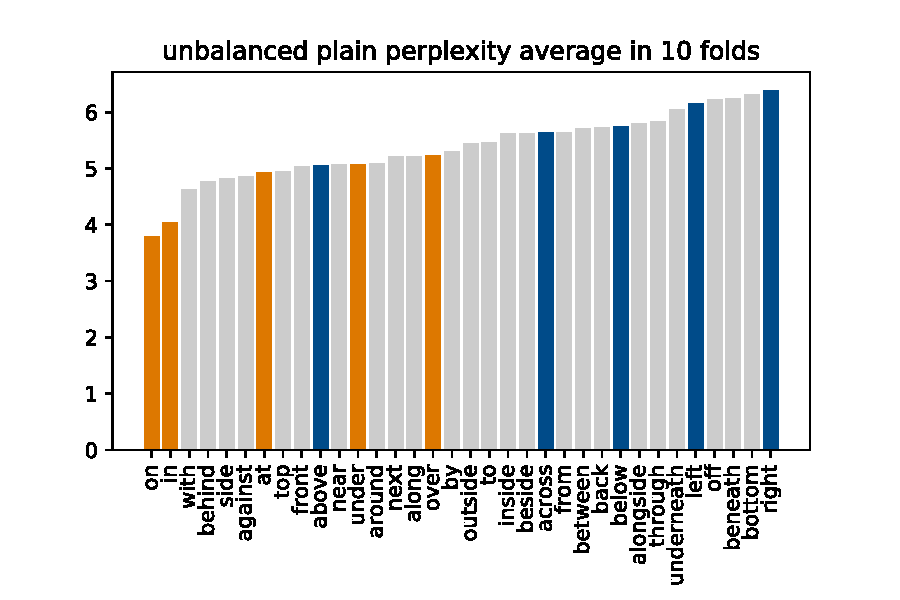
\includegraphics[width=1.12\linewidth]{studies/splu2018/figures/o_pp_cv-avg.pdf}\\
	  	(a) test-set 
    \end{minipage}%
	\begin{minipage}{0.5\linewidth}
		\centering
		\hspace*{-1.em}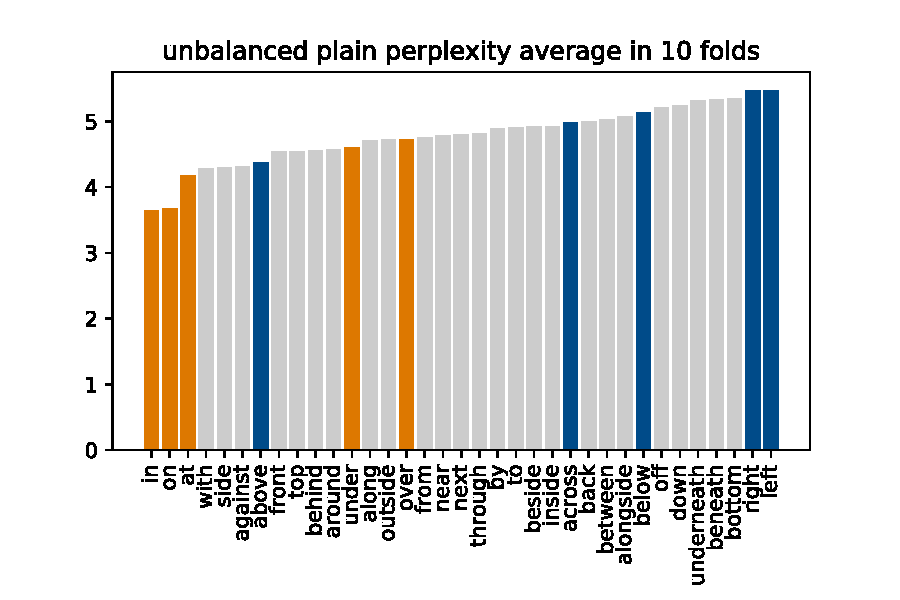
\includegraphics[width=1.12\linewidth]{studies/splu2018/figures/o_train_pp_cv-avg.pdf}\\
		(b) training set
    \end{minipage}%
  \caption{Mean perplexities of spatial descriptions of LM1 (orange:
    functionally biased, blue: geometrically biased relations).}
  \label{splu2018:fig:fig-plain-original}
\end{center}
\end{figure}


\begin{figure}[ht]
  \begin{center}
    \begin{minipage}{0.5\linewidth}
	    \centering
	    \hspace*{-1.2em}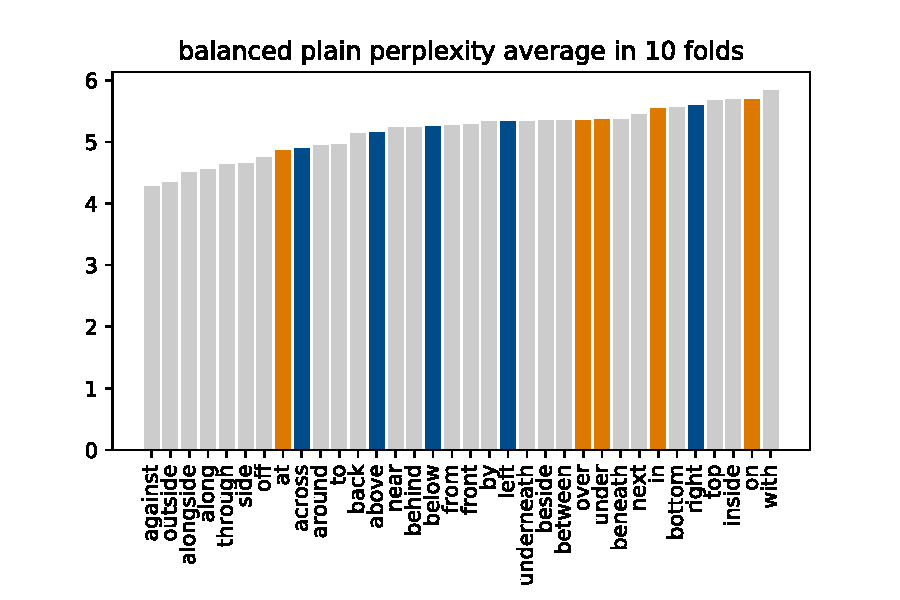
\includegraphics[width=1.12\linewidth]{studies/splu2018/figures/b_pp_cv-avg.pdf}\\
		(a) test-set 
    \end{minipage}%
    \begin{minipage}{0.5\linewidth}
	    \centering
	    \hspace*{-1.em}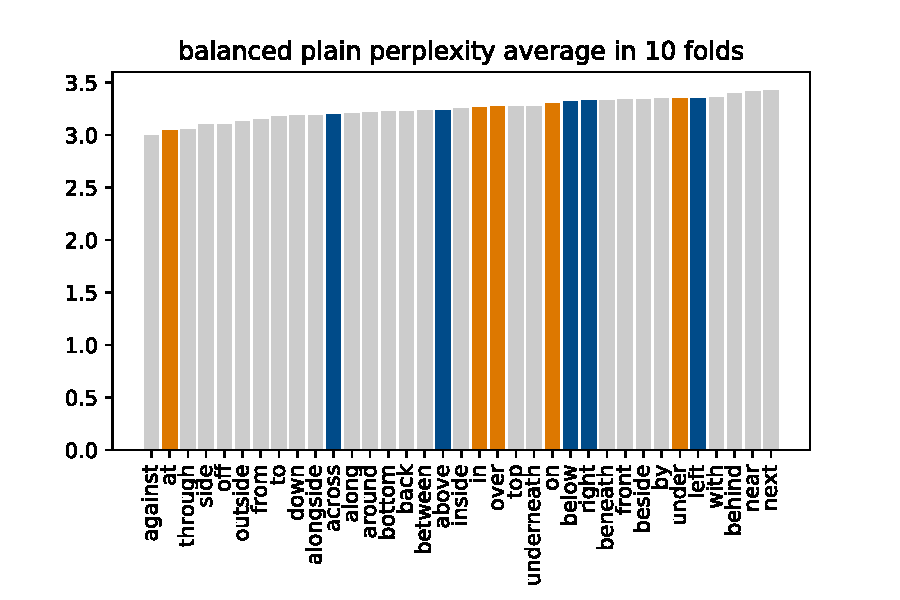
\includegraphics[width=1.12\linewidth]{studies/splu2018/figures/b_train_pp_cv-avg.pdf}\\
	    (b) training set
     \end{minipage}%
  \caption{Mean perplexities of LM2 by spatial relation (orange:
    functionally biased, blue: geometrically biased).}\label{splu2018:fig:fig-plain-balanced}
\end{center}
\end{figure}

Figure~\ref{splu2018:fig:fig-plain-original} shows the estimated average
perplexities of a subset of spatial relations, those that satisfy the sampling frequency requirement described in Section~\ref{splu2018:sec:plain-perplexity-method}. Functionally and geometrically
biased spatial relations as identified experimentally in
the literature (Section~\ref{splu2018:sec:spatial-descriptions}) are
represented with orange and blue bars respectively. There is a tendency
that functionally biased relations lead to lower mean perplexity of
phrases (Hypothesis 2 is confirmed) and also that there is a tendency that spatial
relations of a particular bias cluster together (Hypothesis 1 is also confirmed). We report results both on the training set and the test set which show the same tendencies. This means that our model generalises well on the test set and that the latter is representative.











However, in the language model the perplexities are biased by the
frequency of individual words: more frequent words are more likely and
therefore they are
associated with lower LM perplexity. %
The results show high Spearman's rank correlation coefficient $\rho=0.90$ between frequencies of spatial relation in the dataset and the perplexity of the model on the test set:
on (329,529)
$>$ in (108,880)
$>$ under (11,631)
$>$ above (8,952)
$>$ over (5,714)
$>$ at (4,890)
$>$ below (2,290)
$>$ across	(1,230)
$>$ left (996)
$>$ right (891). For the purposes of our investigation in predictability of target-landmark pairs (Hypothesis 3) we should avoid the bias in the training set.
In order to exclude the
bias of frequencies of relations, we evaluate LM2 where spatial relations are presented with equal frequencies in training. %
Figure~\ref{splu2018:fig:fig-plain-balanced} shows the ranking of spatial
relations by the perplexities when the language model was trained with
balanced frequencies. The two kinds of spatial relations are less clearly separable as the colours overlap (Hypothesis 3 is not confirmed). In comparison to Figure~\ref{splu2018:fig:fig-plain-original} there is an observable trend that all instances
lead to lower perplexities in the training set which is the effect of down-sampling on vocabulary size. Figure~\ref{splu2018:fig:fig-plain-balanced} also shows that phrases with geometrically biased spatial relations have a higher change towards lower perplexities.


Noting that the frequency of using functionally-biased spatial relations are higher in English, this bias and our strong hypothesis for predictability of target-landmark pairs can be expressed with simple joint probabilities which we are estimating with the language model:
\begin{align*}
  P(\mathrm{target, relation, landmark}) = P(\mathrm{relation}) P(\mathrm{target, landmark | relation})
\end{align*}
It is possible that targets and landmarks that occur with
these relations are very specific to these relations but
infrequent with other relations. When we remove their frequency
support provided by the frequency of relations
these targets and landmarks become infrequent in the dataset and
therefore less probable which on overall results in higher
perplexities of phrases with functionally-biased relations. Specificity of targets and landmarks can be a source of these results.


\begin{figure*}[htbp]
	\centering
  \begin{minipage}{.5\linewidth}
    \centering
    \hspace*{-1.2em}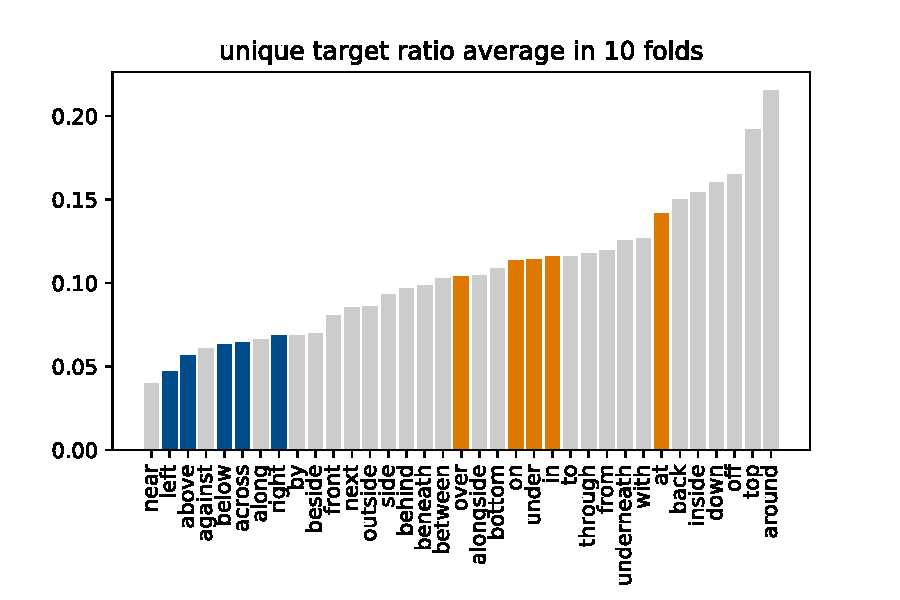
\includegraphics[width=1.12\columnwidth]{studies/splu2018/figures/train_unique_ratio-targets-avg.pdf} \\
    (a) targets
  \end{minipage}%
  \begin{minipage}{.5\linewidth}
    \centering
    \hspace*{-1.em}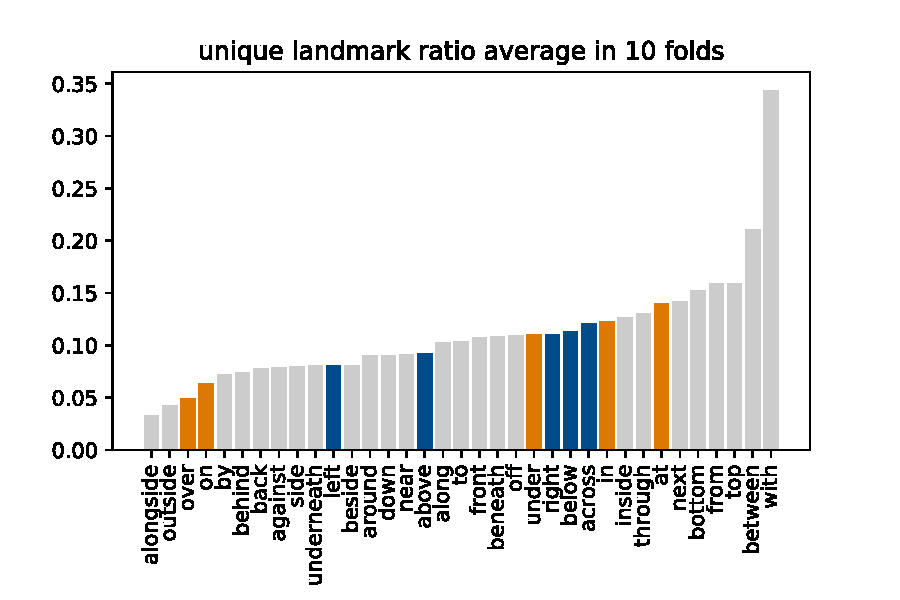
\includegraphics[width=1.12\columnwidth]{studies/splu2018/figures/train_unique_ratio-landmarks-avg.pdf} \\
    (b) landmarks
  \end{minipage}%
  \caption{Ratio between unique types and all types per spatial relation in the balanced dataset for LM2.}\label{splu2018:fig:unique-in-plain-balanced}
\end{figure*}


To provide
(some) evidence for this assumption,
Figure~\ref{splu2018:fig:unique-in-plain-balanced} shows the average ratios of
unique types over total types of targets and landmarks in the balanced
dataset over 10-folds on which LM2 was trained. There is a very clear
division between functionally and geometrically biased spatial
relations in terms of the uniqueness of targets, functionally-biased
relations are occurring with more unique ones which contributes to
higher perplexity of LM2. There is less clear distinction between the
two kinds of spatial relations in terms of uniqueness of
landmarks. Some functional relations such as \emph{on} occur with fewer
unique landmarks than targets (from .11 to .06), some geometric
relations such as \emph{right} occur with more unique landmarks than
targets (from .07 to .11). The asymmetry between targets and landmarks
is expected since the choice of landmarks in the image description
task is restricted by the choice of the targets (as well as other
contextual factors such as visual salience). They have to be ``good
landmarks'' to relate the targets to. A functional relation-landmark
pair is more related to the target through the landmark's affordances
whereas a geometric relation-landmark pair is more related to the
target through geometry. This might explain for example, why \emph{on}
has fewer, but \emph{right} has more unique landmarks than targets. On
the other hand there are also relations where the ratio of unique
targets and landmarks is very similar, for example \emph{at} (.14 and
.14). Overall, it appears that if uniqueness of objects is
contributing to the perplexity of the language model of phrases which
functionally-biased relations (which in this balanced dataset is the
case) then this is more contributed by targets rather than the
landmarks.

To further explore the idea of asymmetry between targets and landmarks
we re-arranged the targets and landmarks in the descriptions from the
balanced dataset that LM2 was trained to \texttt{$<$s$>$ landmark
  relation target $<$/s$>$} and trained LM2$'$. The average
perplexities over 10-folds of cross-validation are shown in
Figure~\ref{splu2018:fig:b_pp_cv-reversed-avg}. Comparing
Figure~\ref{splu2018:fig:b_pp_cv-reversed-avg} with
Figure~\ref{splu2018:fig:fig-plain-balanced} we first observe that the
perplexity of LM2$'$ on the descriptions is overall several magnitudes
lower than the perplexity of LM2 (max 0.06, max 140). Secondly, we
observe that the perplexities of phrases containing different
relations are very similar and that there is no separation of phrases
by perplexity depending on the relation bias. The results are in line
with our argument above. Knowing the landmark, it is much easier for
the language model to predict the relation (of either kinds) and the
target.


\begin{figure}[htbp]
  \begin{center}
  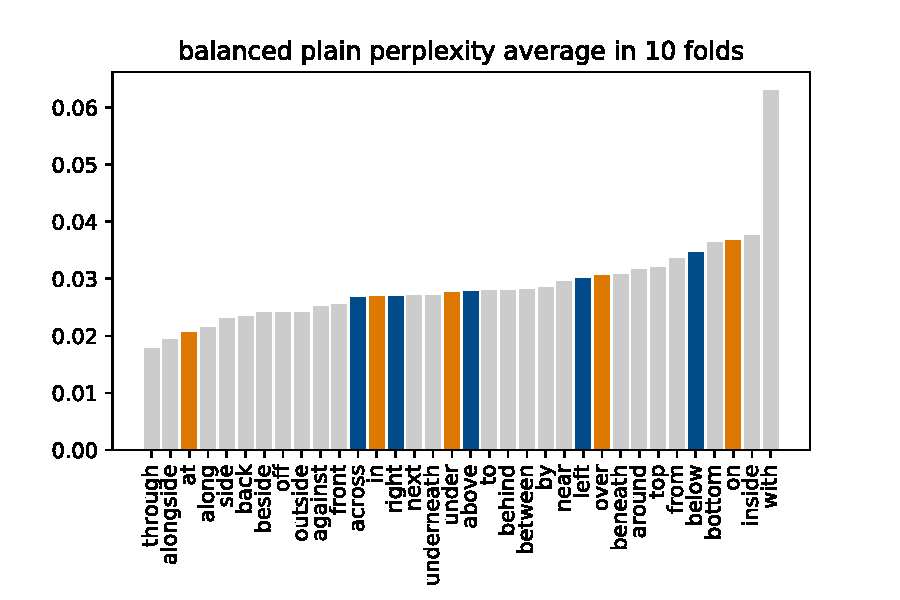
\includegraphics[width=0.6\linewidth]{studies/splu2018/figures/b_pp_cv-reversed-avg.pdf}
  \caption{Mean perplexities of LM2$'$ by spatial relation (orange: functionally biased, blue: geometrically biased)}\label{splu2018:fig:b_pp_cv-reversed-avg}
\end{center}
\end{figure}


In conclusion, the explanation why descriptions with
functionally-biased relations have a higher perplexity than
descriptions with geometrically-biased descriptions appears to be
twofold: (i) functionally-biased relations are more selective of their
targets as expressed by the uniqueness counts, and (ii) functional
relations are also more selective of their landmarks but this fact
works against the performance of the language model. As it is trained
on the sequence left to right, it has to learn to predict relations
only on the basis of targets which in the case of functionally-biased
relations are represented by more unique tokens than
geometrically-biased relations. The more informative words, the
landmarks, that would enable the language model to predict a
functional relation, comes last, after the relation has already been
seen. The possible reason why geometrically-biased relations lead to
lower perplexities of a language model on descriptions is because they
have fewer unique targets. Hence, our Hypothesis 1 which linked
selectivity of functionally-biased relations to low perplexity of
phrases can be refuted. In spatial relations the order of the semantic
interpretation of tokens (that we want to capture in these
experiments) is different from the linear syntactic order of order
which can be captured by the language model. When this order is
changed as in LM2$'$ our predictions come closer to the hypothesis
(Figure~\ref{splu2018:fig:b_pp_cv-reversed-avg}).\footnote{Modulo that
  landmarks are, as discussed above, well-predictive of relations of
  both kinds.} %







By removing the frequency bias on spatial relations in LM2 we fix the
distribution of spatial relations and examine the effect of
distribution of targets and landmarks on perplexities of phrases
(spatial relation as fixed context). In the following section, we fix
the distributions of targets and landmarks of each spatial relation
and examine the perplexity of phrases when another spatial relation is
projected in this context (targets-landmarks as fixed context).





\section{Varying spatial relations}\label{splu2018:sec:swapability}



\subsection{Hypotheses}

Given a particular spatial relation, the distribution of targets and
landmarks that occur with it creates a particular signature of targets
and landmarks, the target-landmark context of a spatial relation. In
this experiment, we investigate the effect on perplexity of phrases
when another spatial relation is projected in such a target-landmark
context. Given different selectivity of functionally- and
geometrically-biased spatial relations, namely the functionally-based
spatial relations are more selective of their targets and landmarks
and therefore create more specific contexts, we should observe
differences in perplexities of phrases when other spatial relations
are projected in these contexts. In particular, we hypothesise that
geometrically-biased spatial relations are more easily swappable than
functionally-biased spatial relations as measured by the perplexity of
a language model trained on the original, non-swapped phrases
(Hypothesis 4).











\subsection{Method}

We use %
LM2 from Section~\ref{splu2018:sec:plain-perplexity} (trained on the balanced
frequencies of spatial relations) with no additional training from the
previous experiment. We group descriptions in the evaluation set by
spatial relation. For each phrase containing a particular spatial
relation, we replace it with every other spatial relation and estimate
the perplexity of the resulting phrase using a language
model. Finally, we calculate the mean of perplexities over all
phrases. We use 10-fold cross-validation and report the final means
across the 10 folds.






\subsection{Results}











\begin{figure}[htbp]
  \begin{center}
  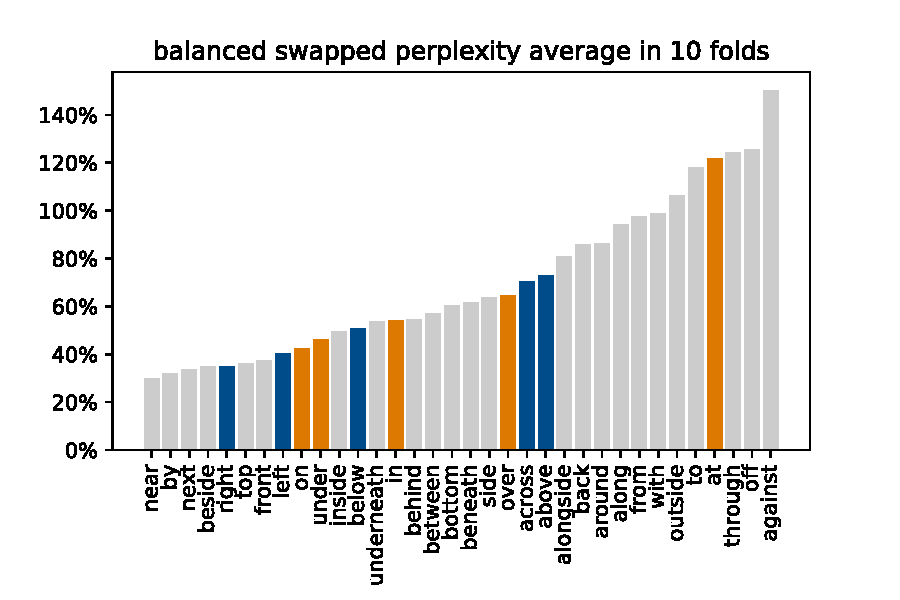
\includegraphics[width=0.6\linewidth]{studies/splu2018/figures/b_swapped_cv-avg.pdf}
  \caption{\%-increase in perplexities of LM2 shown per context of the original preposition when swapped with another one.}
  \label{splu2018:fig:fig-swap-balanced}
\end{center}
\end{figure}


Figure~\ref{splu2018:fig:fig-swap-balanced} shows a \%-increase in mean
complexities from those in Figure~\ref{splu2018:fig:fig-plain-balanced} when
LM2 is applied on phrases with swapped relations in the contexts of
the original relations. Hence, the column ``at'' shows the \%-increase
in perplexities of phrases that originally contained \emph{at} in the
validation dataset but this was replaced by all other spatial
relations. Comparing with Figure~\ref{splu2018:fig:fig-plain-balanced} the
estimated perplexities are higher across all cases which is
predictable. There is a weak tendency that replacing
functionally-biased relations with other relations leads to higher
perplexities of spatial descriptions than replacing
geometrically-biased relations, but the distinction is not
clear cut (Hypothesis 4 partially confirmed). The lack of a clear
distinction between two classes of descriptions confirms our previous
observations about landmarks and targets: the LM has learned
particular contexts for both kinds of descriptions.


















\section{Discussion and conclusion}
\label{splu2018:sec:discussion}


We explored the degree that the functional and geometric character of
spatial relations can be identified by a neural language model by
focusing on spatial descriptions of controlled length and containing
normalised relations. Our first question was about the implications of
using a neural language model for this task. The previous research
\cite{Dobnik:2013aa} used normalised entropy of target-landmarks per
relation and log likelihood ratio between target-landmarks and
relations to test this. These are focused measures that estimate the
variation and the strength of association of words in a corpus. On the
other hand, a language model provides a more general probabilistic
representation of the entire description. As such it captures any kind
of associations between words in a sequence. The other important
observation is that it captures sequential relations in the direction
left to right and as we have seen the sequential nature of the
language model does not correspond precisely with the order in which
semantic arguments of spatial relations are interpreted. However,
nonetheless we can say that language models are able to capture a
distinction between functional and geometric spatial relations (plus
other semantic distinctions) to a similar degree of success as
previously reported measures. Our initial hypothesis about the greater
selectivity of spatial relations for its arguments is correct but it
is exemplified in a greater perplexity of a language model in the
context of balanced spatial relations. We argued that this has to do
with the fact that the targets are more unique to these relations
(which is consequence of a greater specificity for arguments of
functionally biased relations) and is also related to the way a
sequential language model works. In the unbalanced dataset, the
perplexity of the language model is reversed (it is lower with
functionally biased relations) because the specificity of targets to
relations is boosted with greater frequency of functionally-biased
relations. The fact that functionally-biased relations are more
frequent is probably related to the fact that such descriptions are
more informative than purely geometric ones if available for a
particular pair of objects.

We can only report tendencies based on the perplexities of our
language models as our conclusions. This is because the
functional-geometric bias is graded, because the predictions are
highly dependent on the quality and the size of the dataset, and
because other semantic relations might also be expressed by this
measure. We chose a large contemporary dataset of image descriptions
because we hope that it contains a high proportion of prepositions
used as spatial relations. However, there is no guarantee that all
prepositions in this dataset are used this way. We observe that there
is considerable variation of obtained values across the 10-folds of
cross-validation %
and we report the mean values over all folds. As an illustration, in
the supplementary material (Section~\ref{splu2018:sec:evaluation-variation}) we
give an example of graphs from two intermediary folds.


Using a language model in this task we have also learned new insights
about the way language models encode spatial relations in image
descriptions. It has been pointed out (cf. \cite{kelleher2017what}
among others) that convolutional neural networks with an attention
model are designed to detect objects whereas spatial relations between
objects are likely to be predicted by the language model. In this work
we show that language models are not only predicting the relation
(which is expected) but are able to distinguish between different
classes of relations thus encoding finer semantic distinctions. This
tells us that language models are able to encode a surprising amount
of information about world knowledge with a usual caveat that it is
difficult to separate several strands of this knowledge.

The work can be extended in several ways. One way is to study dataset
effects on the predicted results. Datasets with descriptions of
robotic actions and instructions may be particularly promising as they
focus on spatial uses. Different normalisations of spatial relations
have a significant effect on the results. In this work composite
spatial relations such \emph{on the left side of} are normalised to
simple spatial relations such as \emph{left}. However, these could be
treated as separate relations as difference between may exist. A more
systematic examination of clusters of spatial relations would
eventually tell us what other spatial relations not yet identified as
functionally or geometrically biased have similar properties to those
that have identified as such experimentally.






\section*{Acknowledgements}

The research of Dobnik and Ghanimifard was supported by a grant from the Swedish Research Council (VR project 2014-39) for the establishment of the Centre for Linguistic Theory and Studies in Probability (CLASP) at Department of Philosophy, Linguistics and Theory of Science (FLoV), University of Gothenburg.

The research of Kelleher was supported by the ADAPT Research Centre. The ADAPT Centre for Digital Content Technology is funded under the SFI Research Centres Programme (Grant 13/RC/2106) and is co-funded under the European Regional Development Funds.


\section{Appendix: Supplementary material}

\subsection*{Language Model Architecture}\label{splu2018:sec:lm}

\begin{figure}[ht!]
  \begin{center}
  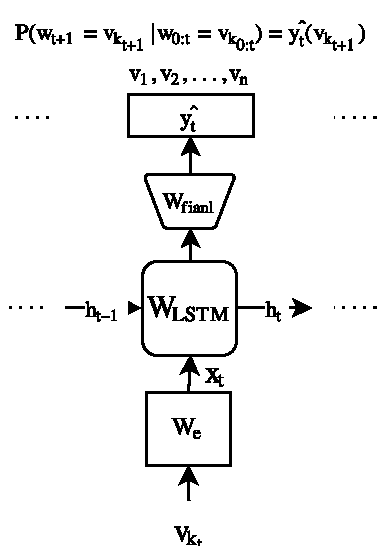
\includegraphics[width=0.35\linewidth]{studies/splu2018/figures/lm_diagram.pdf} \\
  \caption{The recurrent language model diagram with LSTM recurrent unit.}
  \label{splu2018:fig:lm-diagram}
  \end{center}
\end{figure}

The neural language model architecture with the Long-Short Terms Memory (LSTM) function and its parameters, similar to tied weights in \cite{gal2016theoretically}:
\begin{itemize}[topsep=0em,itemsep=0em,partopsep=0em,parsep=0em]
  \item $W_e \in {R}^{n \times d}$ for word embeddings,
  \item $W_{LSTM} \in {R}^{2d \times 4d}$ for parameters of the Long-Short Term
  Memory function,
  \item $W_{Final} \in {R}^{d \times n}$ of the final dense layer with
  \emph{softmax}.
\end{itemize}
\noindent where $n$ is the vocabulary size for $V = \{ v_1, v_2, ..., v_{n} \}$ and $d$
is both the embeddings size and the memory size in LSTM.
For mini-batches from training data, these parameters are being updated using a
stochastic gradient descent to minimise the loss.
\begin{align}\label{splu2018:eq:lm-parameters}
x_{t} &= \delta_{v_{k_t}} \cdot W_e \\
\begin{pmatrix}
\text{i} \\
\text{f} \\
\text{o} \\
\text{g}
\end{pmatrix}
& =
\begin{pmatrix}
\sigma \\
\sigma \\
\sigma \\
\text{tanh}
\end{pmatrix}
\bigg(
\begin{pmatrix}
\text{x}_t \\
\text{h}_{t-1}
\end{pmatrix}
\cdot
\text{W}_{LSTM}
\bigg) \\
c_t & = \text{f} \circ c_{t-1} + \text{i} \circ \text{g} \\
h_t & = \text{o} \circ \text{tanh}(c_t) \\
\hat{y}_t & = \text{softmax}(h_t \cdot \text{W}_{final} + b)
\end{align}
\noindent where $\delta_{v_{k_t}}$ represents the one-hot encoding of the $t$-th word in
the sequence. The $x_{t}$ is the word embedding for this word, and two vectors $c_t$ and $h_t$ represent the states of the recurrent unit. Figure~\ref{splu2018:fig:lm-diagram} illustrates the same equation.

\subsection*{Evaluation}\label{splu2018:sec:evaluation-variation}

\begin{figure}[ht!]
  \centering
  \begin{minipage}{.5\textwidth}
    \centering
    \hspace*{-1.2em}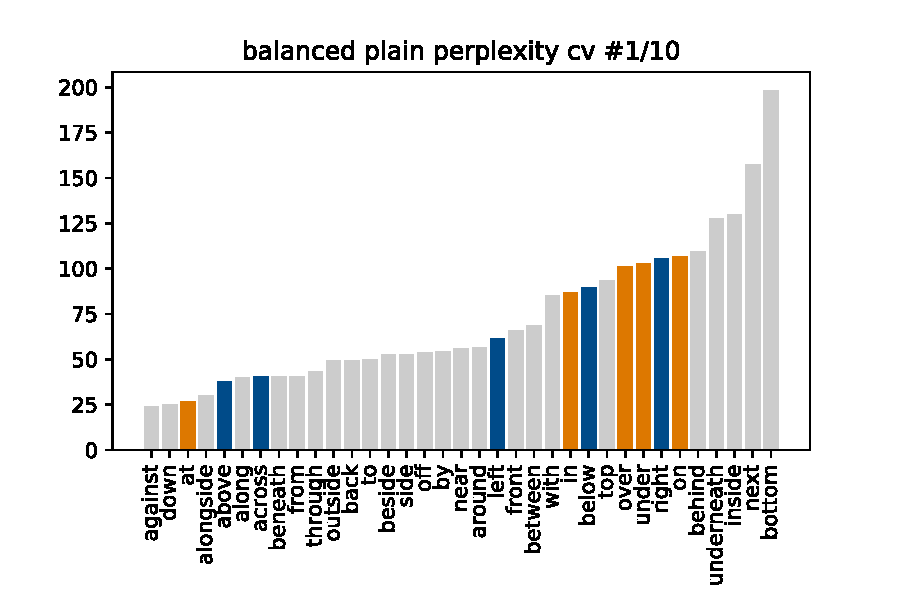
\includegraphics[width=1.12\columnwidth]{studies/splu2018/figures/b_pp_cv-f1.pdf} \\
    (a)
  \end{minipage}%
  \begin{minipage}{.5\textwidth}
    \centering
    \hspace*{-1.em}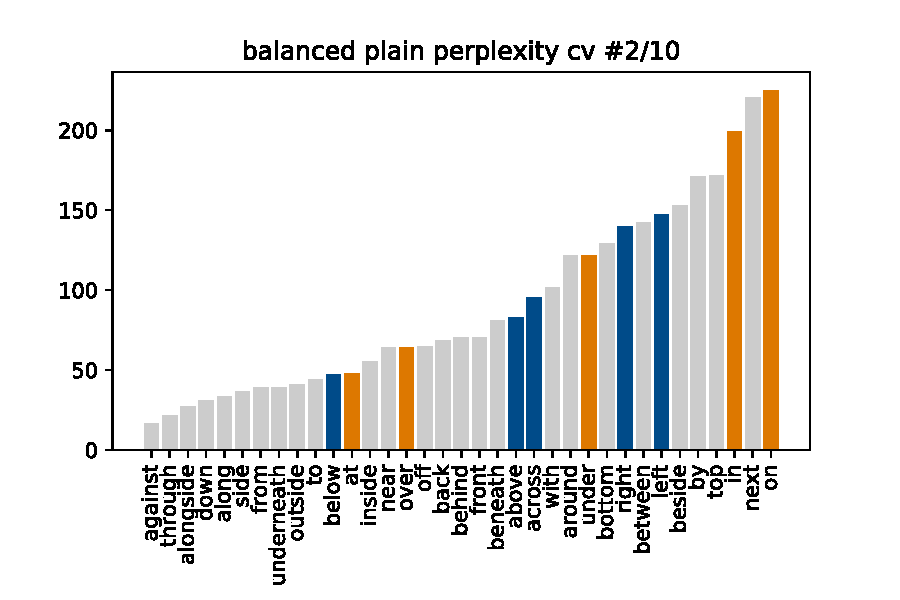
\includegraphics[width=1.12\columnwidth]{studies/splu2018/figures/b_pp_cv-f2.pdf} \\
    (b)
  \end{minipage}
  \caption{Mean perplexities of LM2 by spatial relation for (a) folds 1 and (b) 2 (orange:
    functionally biased, blue: geometrically biased).}\label{splu2018:fig:fig-plain-balanced-folds}
\end{figure}


\clearpage
\bibliographystyle{acl_natbib}
\bibliography{studies/splu2018/references.bib}

\clearpage

\chapter{Representation Of Spatial Relations In Neural Language Models}
\chaptersource{Mehdi Ghanimifard and Simon Dobnik.}{\emph{What} a neural language model tells us about spatial relations,}{In Proceedings of the Combined Workshop on Spatial Language Understanding (SpLU) and Grounded Communication for Robotics (RoboNLP), pp. 71-81. 2019.}

\paragraph{Abstract}
Understanding and generating spatial descriptions requires knowledge about
\emph{what} objects are related, their functional interactions, and \emph{where} the objects are geometrically
located. Different spatial relations have different functional and geometric bias. The wide usage of neural language models in different areas including
generation of image description motivates the study of what kind of knowledge
is encoded in neural language models about individual spatial relations. With the premise
that the functional bias of relations is expressed in their word distributions, we construct multi-word
distributional vector representations and show that these representations
perform well on intrinsic semantic reasoning tasks, thus confirming our premise. A comparison of our vector representations to human
semantic judgments indicates that different bias (functional or
geometric) is captured in different data collection tasks which suggests that the contribution of the two meaning modalities is dynamic, related to the context of the task.



\section{Introduction}

Spatial descriptions such as ``the chair is to the left of the table'' contain
spatial relations ``to the left of'' the semantic representations of which must
be grounded in visual representations in terms of geometry
\cite{harnad1990symbol}. The apprehension of spatial relations in terms of
scene geometry has been investigated through acceptability scores of human
judges over possible locations of objects \cite{logan/sadler:1996}. In
addition, other research has pointed out that there is an interplay between
geometry and object-specific function in the apprehension of spatial relations
\cite{coventry2001interplay}.
Therefore, spatial descriptions must be grounded in two kinds of knowledge \cite{Landau:1993aa,coventry2001interplay,Coventry:2004aa,Landau:2016aa}.
One kind of knowledge is referential meaning, expressed in the geometry of
scenes (geometric knowledge or \emph{where} objects are) while the other kind of knowledge is higher-
level conceptual world knowledge about interactions between objects which is
not directly grounded in perceivable situations but is learned through our
experience of situations in the world (functional knowledge or \emph{what} objects are related).
Furthermore, \citet{coventry2001interplay} argue that individual relations have a
particular geometric and functional bias and
``\emph{under}" and ``\emph{over}" are more functionally-biased than ``\emph{below}" and ``\emph{above}". For instance, when describing the relation between a person and an umbrella in a scene with a textual context such as
``$an~umbrella~\underline{\hspace{0.5cm}}~a~person$", ``\emph{above}" is
associated with stricter geometric properties compared to ``\emph{over}" which
covers a more object-specific extra-geometric sense between the target and
the landmark (i.e. \emph{covering} or \emph{protecting} in this case). Of course, there will be several configurations of objects that could be described either with ``\emph{over}" or ``\emph{above}" which indicates that the choice of a description is determined by the speaker, in particular what aspect of meaning they want to emphasise. %
\citet{coventry2001interplay} consider this bias for prepositions that are geometrically similar and therefore the functional knowledge is reflected in different preferences for objects that are related. However, such functional differences also exist between geometrically different relations.


This poses two interesting research questions for computational modelling of
spatial language. The first one is %
how both kinds of
knowledge interact with individual spatial relations and how models of spatial
language can be constructed and learned within end-to-end deep learning
paradigm. \citet{ramisa2015combining} compare the performance of classifiers
using different multi-modal features (visual, geometric and textual) to predict
a spatial preposition.  \citet{Schwering:2007aa} applies semantic similarity
metrics of spatial relations on geographical data retrieval.
\citet{collell2018acquiring} show that word embeddings can be used as
predictive features for common sense knowledge about location of objects in 2D
images. The second question is related to the extraction of functional
knowledge for applications such as generation of spatial descriptions in a
robot scenario. Typically, a robot will not be able to observe all object
interactions as in \citep{coventry2004spatial} to learn about the interaction of
objects and choose the appropriate relation.
Following the intuition that the functional bias of spatial relations is reflected in a greater selectivity for their target and landmark objects, \citet{Dobnik:2013aa,Dobnik:2014ab} propose that the degree of association
between relations and objects in the corpus of image descriptions can be used as filters for
selecting the most applicable relation for a pair of objects. They also demonstrate that entropy-based
analysis of the targets and landmarks can identify the functional and geometric
bias of spatial relations. They use descriptions from a corpus of image descriptions because here the prepositions in spatial relations are used mainly in the spatial sense. The same investigation of textual corpora such as BNC
\cite{bnc2007british} does not yield such results as there prepositions are used mainly in their non-spatial sense.\footnote{We may call this metaphoric or highly functional usage which is completely absent of the geometric dimension.}
Similarly, \citet{dobnik-etal-2018-exploring} inspect the perplexity of
recurrent language models for different descriptions containing spatial relations %
in the Visual Genome dataset of image captions \cite{krishna2017visual} in order to investigate their bias for objects.

In this paper, we follow this line of work and %
(i) further investigate what semantics about spatial relations are captured
from descriptions of images by generative recurrent neural language models,
and (ii) whether such knowledge can be
extracted, for example as vector representations, and evaluated in tests.
The neural embeddings are opaque to interpretations per se. The benefit of %
using recurrent language models is that they allow us to (i) deal
with spatial relations as multi-word expressions and (ii) they learn their
representations within their contexts:
\begin{itemize}[noitemsep,topsep=0pt,parsep=0pt,partopsep=0pt]
\item[(a)] $a~cat~on~a~mat$
\item[(b)] $a~cat~on~the~top~of~a~mat$
\item[(c)] $a~mat~under~a~cat$
\end{itemize}
\noindent In (a) and (b), the textual contexts are the same
``$a~cat~\underline{\hspace{0.5cm}}~a~mat$" but the meaning of the spatial
relations, one of which is a multi-word expression, are slightly different.
In (c) the context is made different through word order.

The question of what knowledge (functional or geometric) should be represented
in the models can be explained in information-theoretic terms. The low
surprisal of a textual language model on a new text corpora is an indication
that the model has encoded the same information content as the text.
In the absence of the geometric knowledge during the training of the model,
this means that a language model encodes the relevant functional knowledge. We
will show that the degree to which each spatial description containing a
spatial relation encodes functional knowledge in different contexts can be used
as source for building distributional representations. We evaluate these
representations intrinsically in reasoning tests and extrinsically against
human performance and human judgment.

The contributions of this paper are:
\begin{enumerate}[noitemsep] %
\item It is an investigation of the semantic knowledge about spatial relations learned from textual features in recurrent language models with intrinsic and extrinsic methods of evaluation on internal representations.
\item It proposes a method of inspecting contextual performance of generative neural language models over a wide categories of contexts.
\end{enumerate}

This paper is organised as follows: in Section~\ref{splu2019:sec:representations} we
describe how we create distributional representations with recurrent neural language models, in Section~\ref{splu2019:sec:model} we describe our computational
implementations that build these representations, and in Section~\ref{splu2019:sec:experiments} we
provide their evaluation. In Section~\ref{splu2019:sec:conclusions} we give our final
remarks.


\section{Neural representations of spatial relations}\label{splu2019:sec:representations}

Distributional semantic models produce vector representations which capture
latent meanings hidden in association of words in documents
\cite{church1990word,turney2010frequency}.
The neural word embeddings
were initially introduced as a component of neural language models
\cite{bengio2003neural}. However, subsequently neural language models such as
word2vec \cite{mikolov2013distributed} and GloVe \cite{pennington2014glove}
have become used to specifically learn word embeddings from large corpora.
The word embeddings trained by these models capture world-knowledge
regularities expressed in language by learning from the distribution of context
words which can be used for analogical reasoning\footnote{For example, ``$a$ is
to $a^*$ as $b$ is to $b^*$'' can be queried with simple vector arithmetic
$king-man+woman \approx queen$. More specifically, with a search over
vocabulary with cosine similarity:
$\underset{b^* \in V /\{a^*,b,a\}}{arg\,max}\ cos(b^*, a^* - a + b)$ }.
Moreover, sense embeddings \cite{neelakantan2014efficient} and contextual
embeddings \cite{peters2018deep} have shown to provide fine-grained
representation which can discriminate between different word senses or
contexts, for example in substituting synonym words and multi-words in
sentences \cite{mccarthy2007semeval}.



However, meaning is also captured by generative recurrent neural language
models used to generate text rather than predict word similarity. The focus of
our work is to investigate what semantics about spatial relations is captured
by these models. Generative language models use the chain rule of probability
for step-by-step prediction of the next word in a sequence. In these models,
the probability of a sequence of words (or sometimes characters) is defined as
the multiplication of conditional probabilities of each word given the previous
context in a sequence:
\begin{equation}\label{splu2019:eq:lm}
  P(w_{1:T}) = \prod_{t=1}^{T-1}{P(w_{t+1}|w_{1:t})}
\end{equation}
\noindent where $T$ is the length of the word sequence.
The language model estimates the probability of a sequence in
Equation~(\ref{splu2019:eq:lm}) by optimising parameters of a neural network trained
over sufficient data. The internal learned parameters includes embeddings for
each word token which can be used as word level representations directly.

An alternative way of extracting semantic prediction from a generative neural
language model which we are going to explore in this paper is to measure the
fidelity of the model's output predictions against a new ground truth sequence
of words. This is expressed in the measure of \emph{Perplexity} as follows:
\begin{equation}\label{splu2019:eq:pp}
PP(S) =  (\prod_{s \in S}{P(w_{1:t}=s)})^{\frac{-1}{|S|}}
\end{equation}
\noindent where $S$ is a collection of ground truth sentences. Perplexity is a
measure of the difficulty of a generation task which is based on the information
theoretic concept of entropy \cite{bahl1983maximum}. It is based on
\emph{cross-entropy} which takes into account the probability of a sequence of
words in ground truth sentences and the probability of a language model
generating that sequence. It is often used for intrinsic evaluation of word-
error rates in NLP
tasks \cite{chen1998evaluation}.
However, in this paper we use perplexity as a measure of fit of a
pre-trained generative neural language model to a collection of sentences.

Our proposal is as follows. We start with the hypothesis that in spatial
descriptions some spatial relations (those that we call functional) are more
predictable from the associated word contexts of targets and landmarks than
their grounding in the visual features. Hence, this will be reflected in a
perplexity of a (text-based) generative language model trained on spatial
descriptions. Descriptions with functionally-biased spatial relations will be
easier to predict by this language model than geometrically-biased spatial
descriptions and will therefore have lower perplexity. If two sequences of
words where only the spatial relations differ (but target and landmark contexts
as well as other words are the same) have similar perplexity, it means that
such spatial relations have similar selectional requirements and are therefore
similar in terms of functional and geometric bias. We can exploit this to
create vector representations for spatial relations as follows.
Using a dictionary of spatial relations, we extract collections of sentences
containing a particular spatial relation from a held-out dataset not used in
training of the language model.
The collection of sentences with a particular spatial relation are our context
templates.
More specifically, for our list of spatial relations $\{r_1, r_2, ..., r_k\}$,
we %
replace the original relation $r_i$ with a target relation $r_j$ in its
collection of sentences, e.g. we replace \emph{to the right of}$_i$ with
\emph{in front of}$_j$. The outcome is a collection of artificial sentences
$S_{i \to j}$
that are identical to the human-generated sentences except that they contain a substituted
spatial relation. The perplexity of the language model on these sentences
represents the association between the original spatial relation and the
context in which this has been projected:
\begin{equation}\label{splu2019:eq:swapped}
PP(S_{i \to j}) = PP_{i, j} = P(rel_i, c_{rel_j})^{\frac{1}{-N'}}
\end{equation}
\noindent where $c_{rel_j}$ is the context of $rel_i$, and $PP_{i, j}$ is the
perplexity of the neural language model on the sentence collection where
relation $rel_i$ is artificially placed in the contexts of relation $rel_j$. If
$rel_i$ and $rel_j$ are associated with similar contexts, then we expect
low perplexity for $S_{i \to j}$, otherwise the perplexity will be high.
Finally, the perplexity of $rel_i$ against each collection $c_{rel_j}$ is
computed and normalised within each collection (Equation~\ref{splu2019:eq:normal-1}) and
the resulting vector per $rel_i$ over all contexts is represented as a
unit vector (Equation~\ref{splu2019:eq:normal-2}).
\begin{align}
   & & m_{i,j} &= \frac{PP_{i,j}}{\sum_{i'=1}^{k} {PP_{i',j}}}\label{splu2019:eq:normal-1} \\
  \hat{v_i} &= \frac{v_i}{||v_i||} & v_i &= (m_{i,1}, ..., m_{i,k})^T\label{splu2019:eq:normal-2}
\end{align}
\noindent where $\hat{v_i}$ is the vector representation of the relation
$rel_i$. These vectors
create a matrix.
In a particular cell of some row and some column, high perplexity
means that the spatial relation in that row is less swappable with the
context in the column, while a low perplexity means that the spatial relation is highly
swappable with that context. This provides a measure similar to mutual
information (PPMI) in traditional distributional vectors \cite{church1990word}.






In conclusion, representing multi-word spatial relations in a perplexity matrix
of different contexts allows us to capture their semantics based on the
predictions and the discriminatory power of the language model. If all spatial
relations are equally predictable from the language model such vector
representations will be identical and vector space norms will not be able to
discriminate between different spatial relations. In the following sections we
report on the practical details how we build the matrix
(Section~\ref{splu2019:sec:model}) and evaluate it on some typical semantic tasks
(Section~\ref{splu2019:sec:experiments}).
The implementation and evaluation code:
\url{https://github.com/GU-CLASP/what_nlm_srels}

\section{Dataset and models}\label{splu2019:sec:model}

\subsection{Corpus and pre-processing}\label{splu2019:sec:preprocessing}
We use Visual Genome region description corpus \cite{krishna2017visual}. This
corpus contains 5.4 million descriptions of 108 thousand images, collected from
different annotators who described specific regions of each image.
As stated earlier, the reason why we use a dataset of image descriptions is because we want to have spatial
usages of prepositions. Other image captioning datasets such as %
MSCOCO
\cite{lin2014microsoft} and Flickr30k \cite{plummer2015flickr30k} could also be used. However, our investigation has shown that since the task in these datasets in not to describe directly the relation between selected regions,
common geometric spatial relations are almost missing in them: %
there are less
then 30 examples for ``\emph{left of}" and ``\emph{right of}" in these
datasets.

After word
tokenisation with the space operator, we apply pre-processing which removes
repeated descriptions per-image and also descriptions that include uncommon
words with frequency less than 100%
\footnote{The pre-processing leaves 5,042,039 descriptions in the corpus with maximum 31 tokens per sentence. The relatively high threshold of 100 tokens is chosen to insure sufficient support in the 10\% of held-out data for bucketing. We did not use OOV tokens because the goal of the evaluation is to capture object-specific properties about spatial relations and OOV tokens would interfere with this.} %
Then we split the sentences into 90\%-10\%
portions. The 90\% is used for training the language model
(Section~\ref{splu2019:sec:training}), and 10\% is used for generating the perplexity
vectors by extracting sentences with spatial relations that represent our
context bins (Section~\ref{splu2019:sec:contextbins}). The context bins are used for
generating artificial descriptions $S_{i \to j}$ on which the language model is
evaluated for perplexity.%

\subsection{Language model and GloVe embeddings}\label{splu2019:sec:training}

We train a generative neural language model on the 90\% of the extracted corpus
(Section~\ref{splu2019:sec:preprocessing}) which amounts to 4,537,836 descriptions of
maximum length of 29 and 4,985 words in the vocabulary. We implement a
recurrent language model with LSTM \cite{hochreiter1997long} and a word
embeddings layer similar to \citet{gal2016theoretically} in Keras
\cite{chollet2015keras} with TensorFlow \cite{tensorflow2015-whitepaper} as
back-end.
The Adam optimiser \cite{kingma2014adam} is used for fitting the parameters.
The model is set up with 300 dimensions both for the embedding- and the LSTM
units. It is trained for 20 epochs with a batch size of 1024.

In addition to the generative LSTM language model, we also train on the same
corpus GloVe (VG) embeddings with 300 dimensions and a context-window of 5
words. Finally, we also use pre-trained GloVe embeddings on the Common Crawl
(CC) dataset with 42B tokens\footnote{\url{http://nlp.stanford.edu/data/glove.42B.300d.zip}}.


\subsection{Perplexity vectors}\label{splu2019:sec:contextbins}
Based on the lists of spatial prepositions in \citep{Landau:1996aa} and
\citep{herskovits1986language}, we have created a dictionary of spatial relations
which include single word relations as well as all of their possible multi-word
variants. This dictionary was applied on the 10\% held-out dataset where we
found 67 single- and multi-word spatial relation types in total. As their
frequency may have fallen below 100 words due to the dataset split, we further
remove all relations below this threshold which gives us 57 relations.
We also create another list of relations where composite variants such as ``to
the left of'' and ``on the left of'' are grouped together as ``left'' which
contains 44 broad relations.
We group the sentences by the relation they are containing to our
context bins using simple pattern matching on
strings. Table~\ref{splu2019:tab:buckets} contains some examples of our context
bins. The bins are used for artificial sentence generation as
explained in the previous section.

\begin{table}[ht]
    \centering
    \begin{tabular}{r|l}
      Relation ($rel_i$)  & Context bin ($c_{rel_i}$)\\
      \hline
      above     & scissors \underline{\hspace{1.1cm}} the pen \\
                & tall building \underline{\hspace{1.1cm}} the bridge \\
                & $\cdots$\\
      \hline
      below     & pen is \underline{\hspace{1.1cm}} scissors \\
                & bench \underline{\hspace{1.1cm}} the green trees \\
                & $\cdots$\\
      \hline
      next to   & a ball-pen \underline{\hspace{1.1cm}} the~scissors \\
                & car \underline{\hspace{1.1cm}} the water \\
                & $\cdots$\\
    \end{tabular}
	\vspace{0.5em}
    \caption{Examples of context bins based on extracted descriptions from Visual Genome. The images that belong to these descriptions are shown in %
	Appendix~B.
	}\label{splu2019:tab:buckets}
\end{table}


\begin{figure}
  \begin{center}
  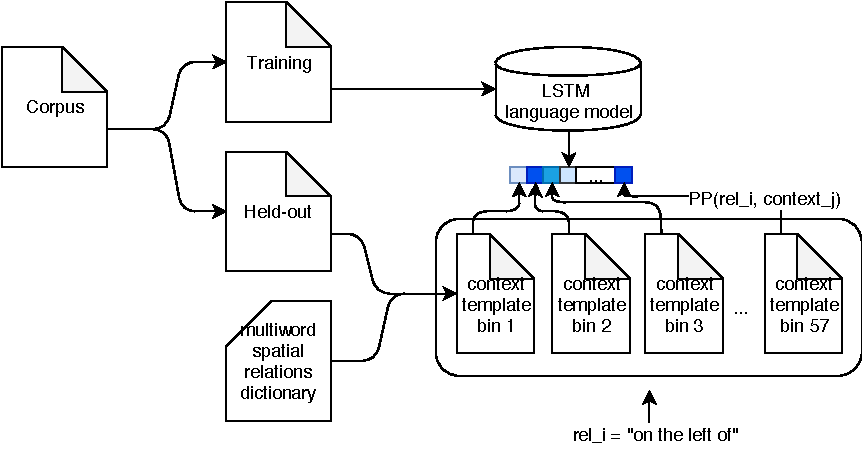
\includegraphics[width=0.75\linewidth]{studies/splu2019/figures/Spatial_Emb_Diagram.pdf}
  \caption{Generating perplexity-based vectors for each spatial relation.}\label{splu2019:fig:diagram}
  \end{center}
\end{figure}

For each of the 67 spatial relations extracted from the larger corpus, there
are 57  collections of sentences (=the number of relations in the smaller
corpus).
Hence, there are
$3,819 (= 67 \times 57)$ possible projections $S_{i \to j}$, where a relation
$i$ is placed in the context $j$, including the case where there is no swapping of relations when $j=i$.  The process is shown in
Figure~\ref{splu2019:fig:diagram}. The vector of resulting perplexities in different
contexts is normalised according to Equation~\ref{splu2019:eq:normal-2} which gives us
perplexity vectors (P-vectors) as shown in Figure~\ref{splu2019:fig:matrix28x26}.

\begin{figure}[ht]
  \begin{center}
  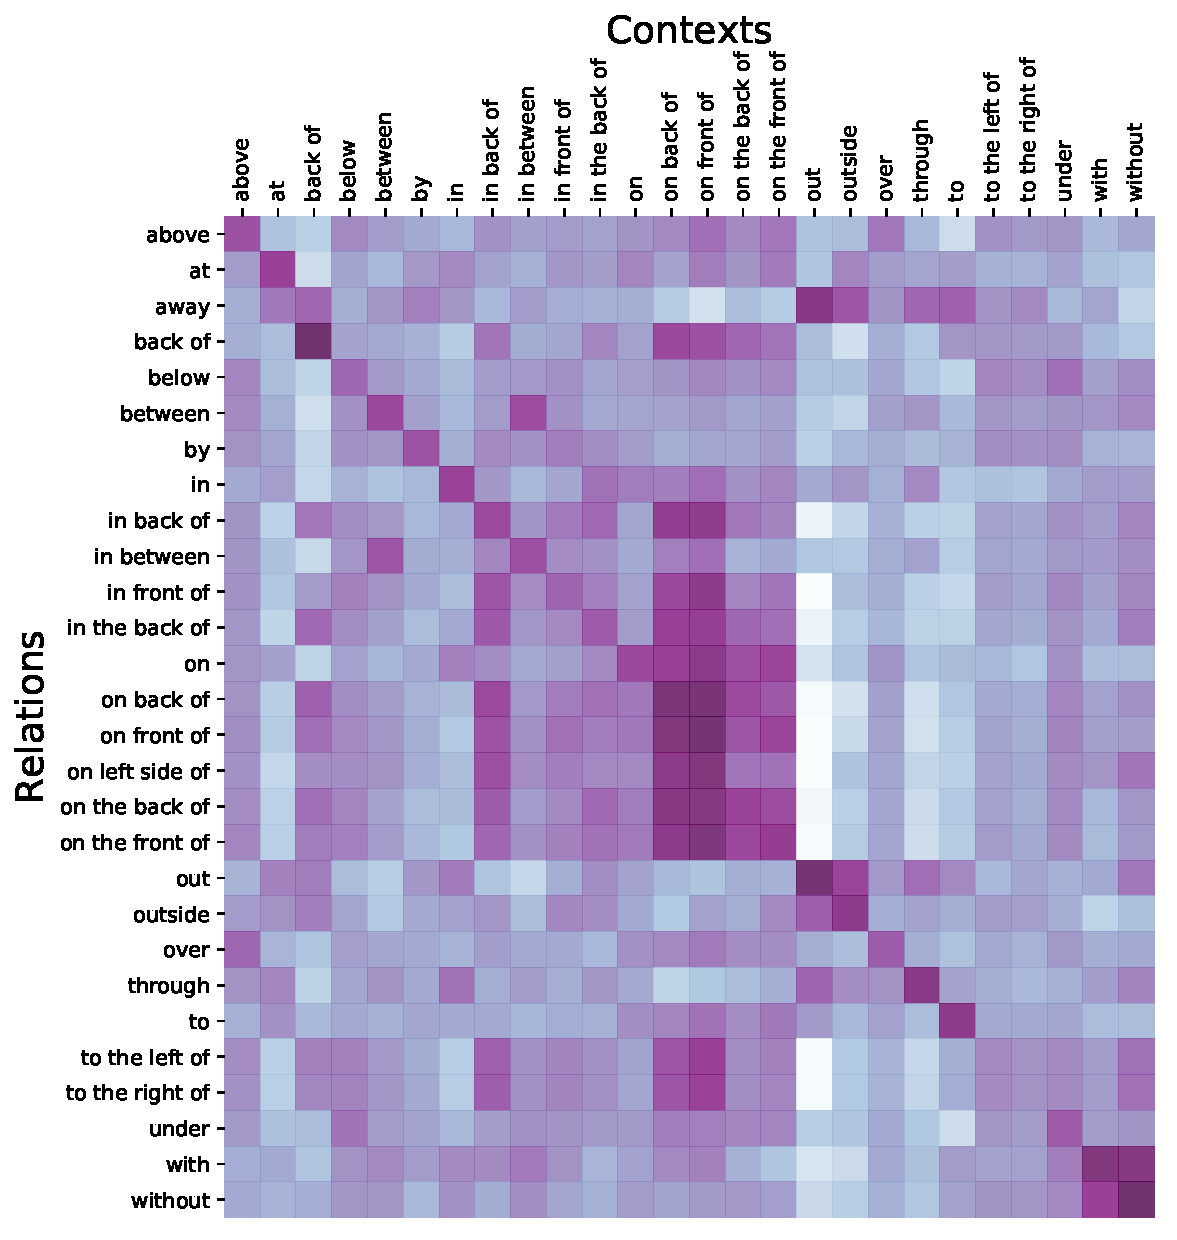
\includegraphics[width=0.75\columnwidth]{studies/splu2019/figures/overall_matrix28x26.pdf}
  \caption{A matrix of perplexity vectors for 28 spatial relations and 26 contexts. For the full $67\times 57$ matrix see %
Appendix~C. The rows represent spatial relations and columns represent the normalised average perplexity of a language model when this relation is swapped in that context.}\label{splu2019:fig:matrix28x26}
  \end{center}
\end{figure}

In addition to the P-vectors we also create representations learned by the word
embedding layer in the generative language model that we train.
For each of the 44 broad single-word spatial relations
we extract a 300-dimensional embedding vector from the pre-trained recurrent
language model (LM-vectors). In order to produce LM-vectors for the multi-word
spatial relations, we %
simply sum the
embeddings of the individual words. For example the embedding vector for ``to
the left of'' is $v_{to} + v_{the} + v_{left} + v_{of}$. The same method is
also used for the GloVe embeddings.


\subsection{Human judgments}\label{splu2019:sec:humanjudgments}
In order to evaluate our word representations we compare them to three sources
of human judgments. The first one are judgments about the the fit of each
spatial relation over different geometric locations of a target object in
relation to a landmark which can be represented as spatial templates
\cite{logan/sadler:1996}. The second are 88,000 word association judgments by English speakers from
\cite{de2018small}. %
In each instance participants were presented a
stimulus word and were asked to provide 3 other words. The dataset contains 4
million responses on 12,000 cues. Based on the collective performance of annotators, the
dataset provides association strengths between words (which contain any kind of
words, not just spatial words) as a measure of their semantic relatedness.
Finally, we collected a new dataset of word similarity judgments using Amazon
Mechanical Turk. Here, the participants were presented with a pair of spatial
relations at a time. Their task was to use a slider bar with a numerical
indicator to express how similar the pair of words are. The experiment is
similar to the one described in \cite{logan/sadler:1996} except that in our
case participants only saw one pair of relations at a time rather than the entire list. The
shared vocabulary between these three datasets covers \emph{left},
\emph{right}, \emph{above}, \emph{over}, \emph{below}, \emph{under},
\emph{near}, \emph{next}, \emph{away}.

\section{Evaluation}\label{splu2019:sec:experiments}


As stated in Section~\ref{splu2019:sec:representations} the P-vectors we have built are
intended to capture the discriminatory power of a generative language model to
encode and discriminate different spatial relations, their functional bias. In
this section we evaluate the P-vectors on several common intrinsic and
extrinsic tests for vectors. If successful, this demonstrates that such
knowledge has indeed been captured by the language model. We evaluate both
single- and multi-word relations.


\subsection{Clustering}
\paragraph{Method} Figure~\ref{splu2019:fig:matrix28x26} and its complete version in %
Appendix~C
show that different spatial relations have
different context fingerprints. To find similar relations in this matrix we can use
\emph{K-means clustering}. %
K-mean is a non-convex problem: different random initialisation may lead to
different local minima.
We apply the clustering on 67 P-vectors for multi-word spatial relations
and qualitatively examine them for various sizes $k$. The optimal number of
clusters is not so relevant here, only that for each $k$ we get reasonable
associations that follow our semantic intuitions.

\paragraph{Results} As shown in Table~\ref{splu2019:tab:clusters}, with $k=30$, the
clustering of perplexity vectors shows acceptable semantics of each cluster.
There are clusters with synonymous terms such as (\ref{item:over}.
\emph{above}, \emph{over}) or (\ref{item:under}. \emph{below}, \emph{under}).
Some clusters have variants of multi-word antonymous such as (\ref{item:topof}.
\emph{on the top of}, \emph{on the bottom of}). Other clusters have a mixture
of such relations, e.g. (\ref{item:leftof}. \emph{right}, \emph{back},
\emph{left}, \emph{side}, and \emph{there}).

\begin{table}
    \begin{tabular}{r|l}
      \begin{minipage}[b]{0.25\linewidth}%
      \begin{footnotesize}
        \begin{enumerate}[noitemsep,topsep=0pt,parsep=0pt,partopsep=0pt]
          \item  to
          \item  on
          \item  away
          \item  here
          \item  into
          \item  from
          \item  during
          \item  back of
          \item  through
          \item  alongside
          \item  along side
          \item  underneath
          \item  in; against
          \item  in front of
          \item \label{item:over} above; over
          \item  to the side
          \item  onto; toward
        \end{enumerate}
      \end{footnotesize}
      \end{minipage}& %
      \begin{minipage}[b]{0.65\linewidth}%
        \begin{footnotesize}
          \begin{enumerate}[noitemsep,topsep=0pt,parsep=0pt,partopsep=0pt]\setcounter{enumi}{17}
            \item  up; down; off
            \item  with; without
            \item  together; out
            \item  outside; inside
            \item  near; beside; by
            \item  top; front; bottom
            \item  in between; between
            \item  along; at; across; around
            \item \label{item:under} beneath; below; under; behind
            \item  \label{item:leftof} right; back; left; side; there
            \item  to the left of; to the right of; next to
            \item  in back of; in the back of; on the back of; at the top of
            \item \label{item:topof} on the top of; on side of; on the bottom of; on left side of; on top of; on the front of; on back of; on the side of; on front of; on bottom of
          \end{enumerate}
        \end{footnotesize}
        \end{minipage}\tabularnewline
    \end{tabular}
	\vspace{0.5em}
    \caption{K-means clusters of spatial relations based on their P-vectors.} %
    \label{splu2019:tab:clusters}
\end{table}

\paragraph{Discussion}  The inspection of the perplexities of two of these
clusters in Figure~\ref{splu2019:fig:clusters} shows that the language model has learned
different selectional properties of spatial relations:
\emph{above} and \emph{over} are generally more selective of their own
contexts, while \emph{to the left of} and \emph{to the right of} show a
higher degree of confusion with a variety of the P-vector contexts.
High degree of confusion in \emph{left} and \emph{right} is consistent with the
observation in \cite{Dobnik:2013aa} that these relations are less dependent on the functional
relation between particular objects and therefore have a higher geometric bias.
On the other hand, \emph{above} and \emph{over} seem to be more selective of
their contexts. The functional distinction between \emph{above} and \emph{over}
is mildly visible: the shades of blue in
\emph{above} are slightly darker than \emph{over}.

\begin{figure}
  \begin{center}
    \begin{minipage}{\linewidth}
      \begin{center}
        \hfill
        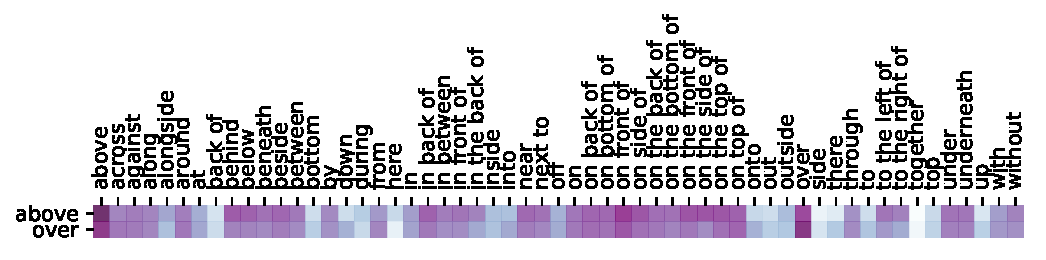
\includegraphics[scale=0.6]{studies/splu2019/figures/above-over.pdf} \\
      \end{center}
    \end{minipage}\\
    \begin{minipage}{\linewidth}
      \begin{center}
        \hfill
        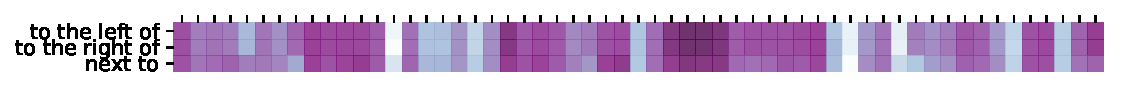
\includegraphics[scale=0.6]{studies/splu2019/figures/left-right.pdf} \\
      \end{center}
    \end{minipage}%
  \caption{The P-vectors of two clusters.
  }
  \label{splu2019:fig:clusters}
\end{center}
\vspace{-5mm}
\end{figure}

\subsection{Analogical reasoning with relations}\label{splu2019:sec:alanogical}
The intrinsic properties of vector representations (the degree to which they
capture functional associations between relations and their objects) can be
tested with their performance in analogical reasoning tasks.
We compare the performance of the P-vectors (Section~\ref{splu2019:sec:contextbins}),
the embeddings of the language model used to create the P-vectors and GloVe
embeddings (Section~\ref{splu2019:sec:training}) in two
analogical tasks which require both geometric and functional reasoning.

\subsubsection{Predicting analogical words}

\paragraph{Method}
The task is similar to the analogy test
\cite{mikolov2013distributed,levy2015improving} where two pairs of words are
compared in terms of some relation ``$a$ is to $a'$ as $b$ is to $b'$".
We manually grouped spatial relations that are opposite in one geometric
dimension to 6 groups.
These are: Group 1: left, right; Group 2: above, below; Group 3: front,
back; Group 4: with, without; Group 5: in, out; and Group 6: up, down.
We generate all possible permutations of these words for the analogical
reasoning task which gives us 120 permutations. We expand these combinations to
include multi-word variants. This dataset has 85,744 possible analogical
questions such as (\emph{above} :: \emph{below}, \emph{to the left of} :: ?).
We accept all variants of a particular relation (e.g.
\emph{to the right side of} and \emph{to the right of}) as the correct answer.




\paragraph{Results} As shown in in Table~\ref{splu2019:tab:analogy}, on the single-word
test suite, the LM-embeddings perform better than other models. On multi-word
test suite the P-vectors perform slightly better. On both test suites, GloVe
trained on Common Crawl performs better than GloVe trained on Visual Genome.
However, its performance on multi-word relations is considerably lower. We
simulated random answers as a baseline to estimate the difficulty of the task.
Although the multi-word test suite has $\sim 700$ times more questions than the
test suite with single-word relations, it is only approximately 2-times more
difficult to predict the correct answer in the multi-word dataset compared to
the single-word dataset.

\begin{table}
    \centering 
      \begin{tabular}{l|r|r}
              & Single word & Multi-words \\
      \hline
      GloVe (CC)   & 0.56 & 0.36 \\
      GloVe (VG)   & 0.43 & 0.29 \\
      \hline
      LM           & 0.86 & 0.45 \\
      P-vectors & 0.62 & 0.47 \\
      \hline
      Random       & 0.11 & 0.05 \\
      \end{tabular}
  	  \vspace{0.5em}
      \caption{The accuracies of different representations on the word analogy test.}
      \label{splu2019:tab:analogy}
      \vspace{-5mm}
\end{table}

\paragraph{Discussion} The perplexity of the language model on complete context
phrases (Multi-words) is as good indicator of semantic relatedness as the word embeddings of
the underlying language model and much better than GloVe embeddings. The good
performance of the P-vectors explains the errors of the language model in
generating spatial descriptions. The confusion between \emph{in front of} and
\emph{on the back of} is similar to the confusion between \emph{to the left of}
and \emph{to the right of} in terms of their distribution over functional
contexts. Hence, a similar lack of strong functional associations allows the
vectors to make inference about geometrically related word-pairs. This
indicates that functional and geometric bias of words are complementary. There
are two possible explanations why P-vectors perform better than LM-embeddings
on multi-word vectors: (i) low-dimensions of P-vectors (57D) intensify the
contribution of spatial contexts for analogical reasoning compared to
high-dimensional LM-embeddings (300D); (ii) summing the vectors of the
LM-embeddings for multi-words reduces their discriminatory effect.

\subsubsection{Odd-one-out}

\paragraph{Method}
Based on the semantic relatedness of words, the goal of this task is to find
the odd member of the three.
The ground truth for this test are the following five categories of spatial
relations, again primarily based on geometric criteria:
X-axis: left, right; Y-axis: above, over, under, below; Z-axis: front, back;
Containment: in, out; and Proximity: near, away.
Only the Y-axis contains words that are geometrically similar but functionally
different, e.g. \emph{above}/\emph{over}.
In total there are 528 possible instances with 3,456 multi-word variations. The
difficulty of the task is the same for both single- and multi-word expressions as the choice is always
between three words. Hence, the random baseline is $0.33$.






\paragraph{Results} Table~\ref{splu2019:tab:oddones} shows the accuracy in predicting
the odd relation out of the three. We also add a comparison to fully geometric
representations captured by spatial templates \cite{logan/sadler:1996}.
\citet{Ghanimifard:2017ab} show that spatial templates can be compared with
Spearman's rank correlation coefficient $\rho_{X,Y}$ and therefore we also
include this similarity measure. Since our groups of relations contain those
that are geometric opposites in each dimension, we take the absolute value of
$|\rho_{X,Y}|$.
Spatial templates are not able to recognise relatedness without the right
distance measure, $|\rho_{X,Y}|$.
LM-embeddings perform better than other vectors in both tests, but P-vectors
follow closely. All models have a low performance on the multi-word test suite.
When using $|\rho_{X,Y}|$
all vectors other than P-vectors produce better results. While we do not have
an explanation for this, it is interesting to observe that $|\rho_{X,Y}|$ is a
better measure of similarity than cosine.


\begin{table}
    \centering 
      \begin{tabular}{r|cc|cc}
        & \multicolumn{2}{c|}{Single word} & \multicolumn{2}{|c}{Multi-words} \\
        & $1-cos$ & $|\rho|$ & $1-cos$ & $|\rho|$ \\
      \hline
      GloVe (CC)   & 0.62 & 0.68 & 0.52 & 0.58 \\
      GloVe (VG)   & 0.61 & 0.61 & 0.58 & 0.59 \\
      \hline
      LM           & 0.87 & 0.90 & 0.82 & 0.88 \\
      P-vectors    & 0.72 & 0.70 & 0.64 & 0.52 \\
      \hline
      Sp Templates & 0.22 & 1.0  &  -   &  -   \\
      \end{tabular}
  \vspace{0.5em}
    \caption{The accuracies in odd-one-out tests.}
    \label{splu2019:tab:oddones}
\end{table}


\paragraph{Discussion} The results demonstrate that using functional
representations based on associations of words
can predict considerable information about geometric distinctions between
relations, e.g. distinguishing \emph{to the right of} and \emph{above}, and
this is also true for P-vectors. As stated earlier, our explanation for this is
that functional and geometric knowledge is in complementary distribution.
This has positive and negative implications for joint vision and language
models used in generating spatial descriptions.
In the absence of geometric information, language models provide strong
discriminative power in terms of functional contexts, but even if geometric
latent information is expressed in them, an image captioning system still needs
to ground each description in the scene geometry.



\subsection{Similarity with human judgments}\label{splu2019:sec:extrinsic}
We compare the cosine similarity between words in LM- and P-vector spaces with
similarities from (i) word association judgments \cite{de2018small},
(ii) our word similarity judgments from AMT, and
(iii) spatial templates (Section~\ref{splu2019:sec:humanjudgments}). We take the maximum
subset of shared vocabulary between them, including \emph{on}, \emph{in} only
shared between (i) and (ii).
Since (i) is an association test, unrelated relations do not have association
strengths. There are 55 total possible pairs of 11 words, while only 28 pairs
are present in (i) as shown in Figure~\ref{splu2019:fig:humansim}.


\begin{figure}
  \begin{center}
    \begin{minipage}{0.4\linewidth}
      \begin{center}
      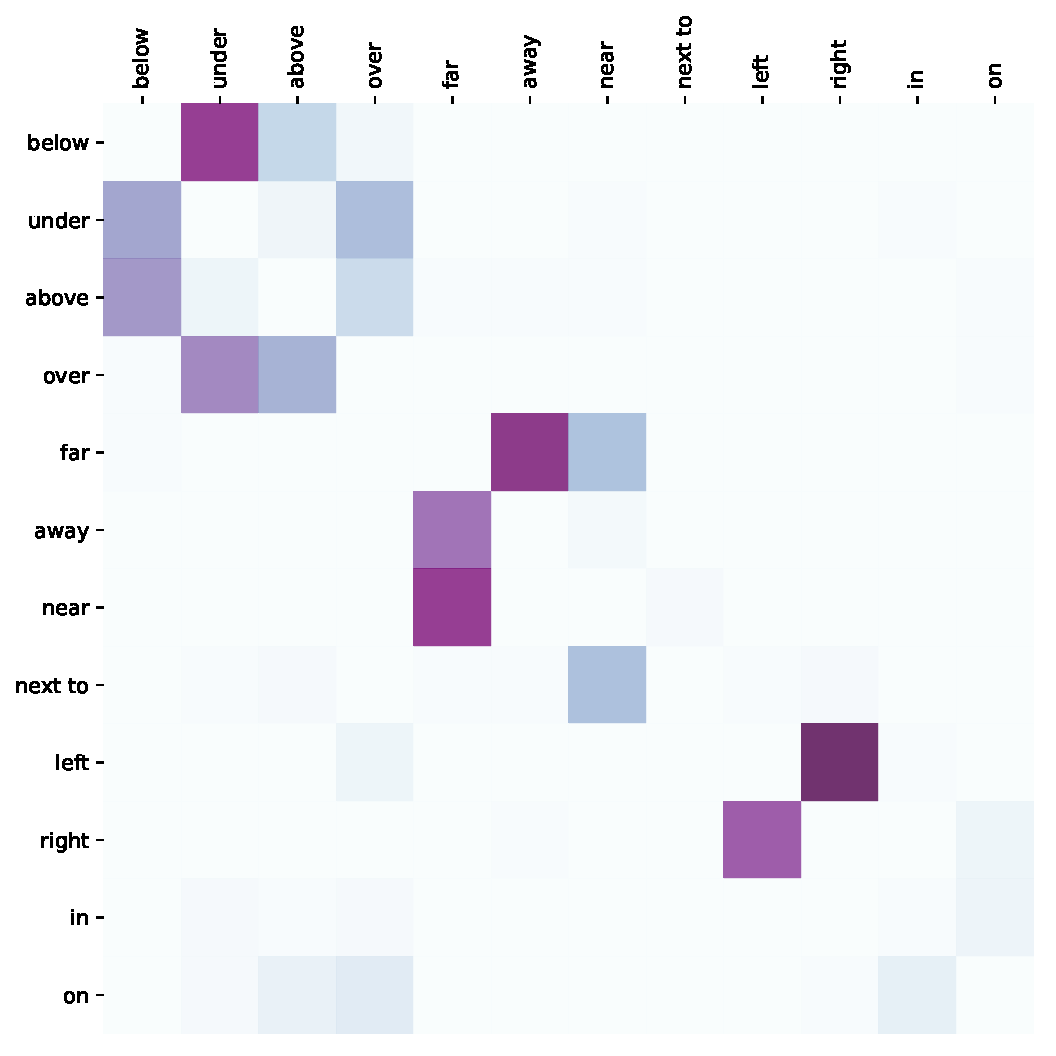
\includegraphics[width=1\columnwidth]{studies/splu2019/figures/word_association_test.pdf} \\
      (a)
      \end{center}%
    \end{minipage}%
    \begin{minipage}{0.4\linewidth}
      \begin{center}
      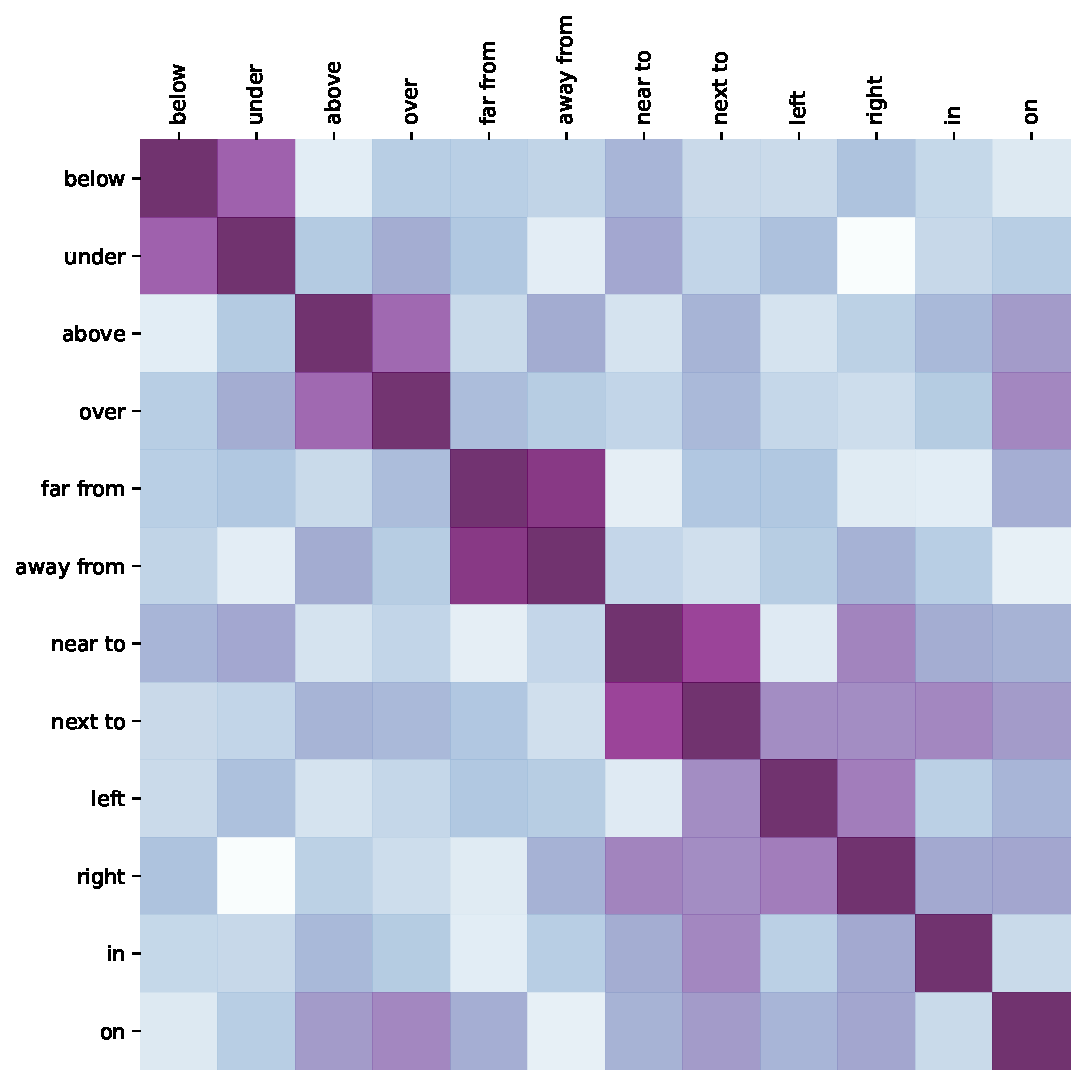
\includegraphics[width=1\columnwidth]{studies/splu2019/figures/relatedness_judgments.pdf} \\
      (b)
      \end{center}%
    \end{minipage}
    \caption{(i) Word association judgments and (ii) word similarity judgments}
  \label{splu2019:fig:humansim}
\end{center}
\end{figure}

\paragraph{Method}
We take the average of the two way association strengths if the association
exists and for (i) %
we assign a zero association for unrelated pairs such as \emph{left} and
\emph{above}. Spearman's rank correlation coefficient $\rho_{X,Y}$ is used to compare the calculated similarities.

\paragraph{Results} Table~\ref{splu2019:tab:humanjudgments} shows ranked
correlations of different similarity measures.
Spatial templates do not correlate with (WA)  word associations and (WS) word
similarities.
On 28 pairs there is a weak negative correlation between spatial templates and
WS. The correlation of similarities of two different human judgments is
positive but weak ($\rho = 0.33$). The similarities predicted by LM-vectors and
P-vectors correlate better with WA than WS.

\begin{table}[ht]
    \centering 
      \begin{tabular}{r|c|c||c|c}
        & \multicolumn{2}{c||}{55 pairs} & \multicolumn{2}{|c}{28 pairs} \\
        \hline
        &
        WA &
        WS &
        WA &
        WS \\
      \hline
      SpTemp & $-0.02$       & $-0.08$ & $0.06$       & $-0.35$ \\
      LM     & $ 0.48^{***}$ & $ 0.15$ & $0.59^{***}$ & $ 0.08$ \\
      P & $ 0.48^{***}$ & $ 0.19$ & $0.40^{**}$  & $-0.08$ \\
      \hline
      \multicolumn{5}{c}{p-values: $* < 0.01$, $** < 0.01$, $*** < 0.001$} \\
      \end{tabular}
	  \vspace{0.5em}
      \caption{
        Spearman's $\rho$ between pairwise lists of similarities.
        WA are similarities based on word associations and WS are direct word
        similarities from human judgments.}
      \label{splu2019:tab:humanjudgments}
\end{table}

\paragraph{Discussion} The low correlation between the two similarities from human judgments
is surprising. Our explanation is that this is because of different priming to
functional and geometric dimension of meaning in the data collection task.
In the WA task participants are not primed with the spatial domain but they are
providing general word associations, %
hence functional associations. On the other hand, in the WS task
participants are presented with two spatial relations, e.g. \emph{left of} and
\emph{right of}, and therefore
the geometric dimension of meaning is more explicitly attended.
We also notice that judgments are not always unison, the same pair may be
judged as similar and dissimilar which further confirms that participants are
selecting between two different dimensions of meaning.
This observation is consistent with our argument that LM-vectors
and P-vectors encode functional knowledge. Both representations correlate
better with WA than with WS.
Finally, \cite{logan/sadler:1996} demonstrate that
WS judgments can be decomposed to dimensions that correlate with the dimensions of the spatial templates. We leave this investigation for our
future work.

\section{Conclusion and future work}\label{splu2019:sec:conclusions}

In the preceding discussion, we have examined what semantic knowledge about spatial relations is captured in
representations of a generative neural language model. In particular, we are
interested if the language model is able to encode a distinction between
functional and geometric bias of spatial relations and how the two dimensions
of meaning interact. The idea is based on earlier work
that demonstrates that this bias can be recovered from the selectivity of
spatial relations for target and landmark objects.
In particular,
(i) we test the difference between multi-word spatial relations at two levels: the
word embeddings which are a form of internal semantic representations in a language model and the
perplexity-based P-vectors which are external semantic representations based on the language model performance;
(ii) we project spatial relations in the contexts of other relations and we
measure the fit of the language model to these contexts using perplexity
(P-vectors);
(iii) we use these contexts to build a distributional model of multi-word
spatial relations;
(iv) in the evaluation on standard semantic similarity tasks, we demonstrate
that these vectors capture fine semantic distinctions between spatial relations;
(v) we also demonstrate that these representations based on word-context associations latently capture geometric knowledge %
that allows analogical reasoning about space; this suggests that functional and geometric components of meaning are complementary: %
(vi) doing so we also demonstrated that generation of
spatial descriptions is also dependent on textual features, even if the system
has no access to the visual features of the scene. This has implications for
baselines for image captioning and how we evaluate visual grounding of
spatial relations.


Our work could be extended in several ways, including by %
(i) using the knowledge about the bias of spatial relations to evaluate captioning
tasks with spatial word substitutions
\cite{shekhar2017vision,shekhar2017foil};
(ii) examining how functional knowledge is complemented with visual knowledge
in language generation \cite{christie2016resolving,delecraz2017correcting}
(iii) using different contextual embeddings such as ELMo \cite{peters2018deep}
and BERT \cite{devlin2018bert}
for the embedding layer of the generative language model rather than our specifically-trained word embeddings; note that P-vectors are representations of collections of context based on the performance of the decoder language model while ELMo and BERT are representations of specific context based on the encoder language model;
(iv) comparing language models for spatial descriptions from different
pragmatic tasks. As the focus of image captioning is to best describe the image
and not for example, spatially locate a particular object, the pragmatic
context of image descriptions is biased towards the functional sense of spatial
relations. Our analysis should be extended
to different kinds of corpora, for example those for visual question answering,
human-robot interaction, and navigation instructions where we expect that precise
geometric locating of objects receives more focus. Therefore, we expect to find a
stronger geometric bias across all descriptions and a lower performance of our representations on analogical
reasoning.

\section*{Acknowledgements}
We are grateful to the anonymous reviewers for their helpful
comments. The research of the authors was supported by a grant from
the Swedish Research Council (VR project 2014-39) to the Centre for
Linguistic Theory and Studies in Probability (CLASP) at Department of
Philosophy, Linguistics and Theory of Science (FLoV), University of
Gothenburg.

\section{Appendix: Perplexity}
\label{splu2019:sec:appendix}
The perplexity in the paper is formulated as follows:
\begin{equation}
PP(S) =  (\prod_{s \in S}{P(w_{1:t}=s)})^{\frac{-1}{|S|}}. \tag{\ref{splu2019:eq:pp}}
\end{equation}
By definition, the perplexity of a model $q$ on a test suit $S$ is defined as follows:
\begin{equation}\label{splu2019:eq:pp_ce}
PP(S) =  2^{H(p,q)}
\end{equation}
\noindent where $H$ is cross entropy, and $p$ is the likelihood of each
possible sample in the test suit. The definition of cross entropy is as follows:
\begin{equation}\label{splu2019:eq:ce}
H(p,q) = - \sum_{x \in S} p(X=x) log_2(q(X=x))
\end{equation}
\noindent where $X$ is a random variable, and $x$ is a possible value of the
random variable. In a forward generative language model, the random variable is
conditioned on the previous words. With test suite being a sequence of words
$S=w_{1:T}$, the likelihood of each word in the sequence is
$p(w_t)=\frac{1}{T}$, and the cross entropy of the model on the samples is:
\begin{align}\label{splu2019:eq:ce_lm}
H(p, q) &= - \sum_{t = 1}^{T}{p(w_t) log_2(q(w_t|w_{1:t-1}))} \\
&= -  \frac{1}{T} \sum_{t = 1}^{T}{log_2(q(w_t|w_{1:t-1}))}
\end{align}
\noindent where $w_t$ is a token at a time $t$, in a sequence with maximum $T$
tokens, $w_{1:t} = w_1, w_2, ..., w_t$.  Therefore the perplexity is:
\begin{align}
PP(S) &= 2^{- \frac{1}{T} \sum_{t = 1}^{T}{log_2(q(w_t|w_{1:t-1}))}}\label{splu2019:eq:pp_ce1} \\
&= (\prod_{t = 1}^{T}{q(w_t|w_{1:t-1})})^{- \frac{1}{T}}\label{splu2019:eq:pp_ce2}
\end{align}
\noindent Equation~\ref{splu2019:eq:pp_ce2} is often used as definition of perplexity in
language models \cite{goodman2001bit} and Equation~\ref{splu2019:eq:pp_ce1} is its
numeric computation to avoid underflow due to adding logits. \\
There are two ways to extend the definition to the case when perplexity is
calculated for a collection of sentences. (i) We can treat the corpus as a long
sequence of tokens and use the previous equations. (ii) We can use
Equation~\ref{splu2019:eq:ce} with a change to the model definition, from a token model
to a sentence model. The benefit of this method is that it assigns the same
likelihood for each sentence regardless of its length. In this case, the chain
rule is used for the sentence model. The likelihood of each sentence is one
over the number of sentences in the test suite, $p(s)=\frac{1}{|S|}$:
\begin{align}\label{splu2019:eq:ce_lm2}
H(p, q) &= - \sum_{s \in S}{p(s) log_2(\hat{P}(s))} \\
&= - \frac{1}{|S|} \sum_{s \in S}{log_2(\hat{P}(s))}
\end{align}
Based on the chain rule, the sentence model can be calculated as follows:
\begin{align}\label{splu2019:eq:lm2}
\hat{P}(w_{1:T}=s) &= \prod_{t = 1}^{T}{q(w_t|w_{1:t-1})} \\ \label{splu2019:eq:lm2logits}
log_2(\hat{P}(w_{1:T}=s)) &= \sum_{t = 1}^{T}{log_2(q(w_t|w_{1:t-1}))}
\end{align}
Perplexity in this case is defined as in Equation~\ref{splu2019:eq:pp} here repeated as
Equation\ref{splu2019:eq:pp2}:
\begin{equation}\label{splu2019:eq:pp2}
PP(S) =  (\prod_{s \in S}{\hat{P}(w_{1:T_s}=s)})^{\frac{-1}{|S|}}
\end{equation}
\noindent which instead of using the product is computed as a sum of
logits from Equation~\ref{splu2019:eq:ce_lm2} and \ref{splu2019:eq:lm2logits}.


\section{Appendix: Examples of images from Visual Genome}\label{splu2019:sec:appendix-image}
Figure~\ref{splu2019:fig:examples1} and Figure~\ref{splu2019:fig:examples2} are the examples from VisualGenome which their region descriptions are used in the paper as examples of relation-context substitution table. 
\begin{figure*}[h!]
	\centering
	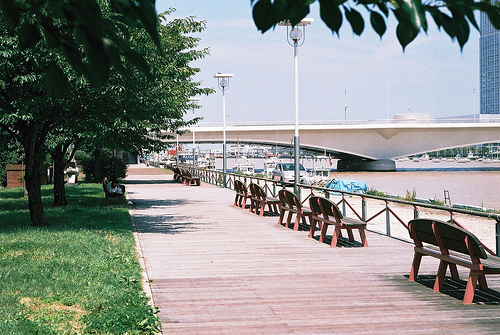
\includegraphics[width=0.65\linewidth]{studies/splu2019/figures/2367586.jpg}
	\caption{
		image\_id = 2367586 \\
		tall building above the bridge \\
		bench below the green trees \\
		car next to the water}\label{splu2019:fig:examples1}
\end{figure*}

\begin{figure*}[h!]
	\centering
	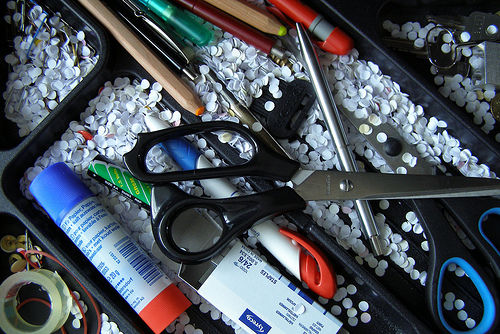
\includegraphics[width=0.65\linewidth]{studies/splu2019/figures/2320485.jpg}
	\caption{
		image\_id = 2320485 \\
		scissors above the pen \\
		the pen is below scissors \\
		a ball-pen next to the scissorts}\label{splu2019:fig:examples2}%
\end{figure*}

\pagebreak
\section{Appendix: Complete P-vectors}\label{splu2019:sec:appendix_plots}
Figure~\ref{splu2019:fig:matrix} is the full presentation of P-vectors.
\begin{figure*}[h!]
	\begin{center}
		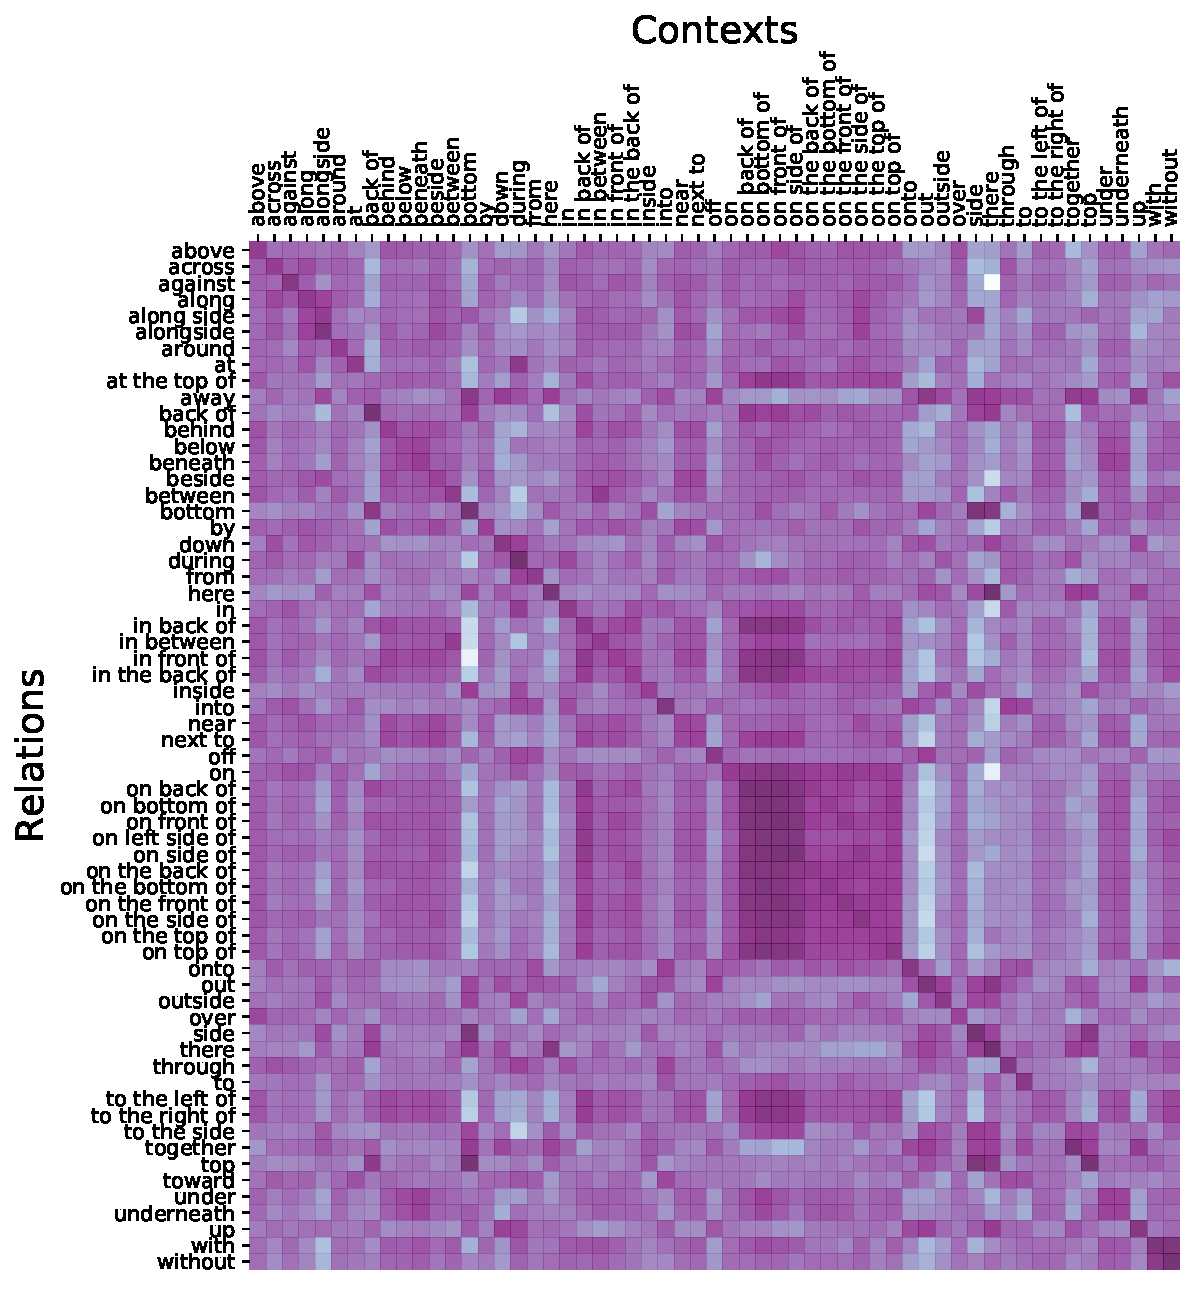
\includegraphics[width=0.9\linewidth]{studies/splu2019/figures/overall_matrix57x63.pdf}
		\caption{Perplexity vectors for 67 spatial relations on 57 context bins.}
		\label{splu2019:fig:matrix}
	\end{center}
\end{figure*}

\section{Appendix: Similarity Judgment Dataset}\label{splu2019:sec:similarity_dataset}
In total 66 worker in Amazon Mechanical Turk annotated the word similarity. For each word pair, we collected 10 judgments. The word pairs vertically in random order were presented to annotators to judge their similarity. The input form was a slider in the web interface which they could freely adjust the indicator position between dissimilar and similar rating (Figure~\ref{splu2019:fig:screenshot}). In order to identify the bad annotators, we randomly asked the annotators to judge similarity between ``\emph{green}" and one of the spatial relations, we also asked similarity judgment between a spatial relation and itself. If the answer to similarity with green was higher than \%60, or the answer for self similarity was lower than \%90, all contributions of that worker were taken out from the dataset. This cleaning technique removed 9 workers in total, which left us about 7 annotation on each word pair.

\begin{figure}[h!]
	\begin{center}
		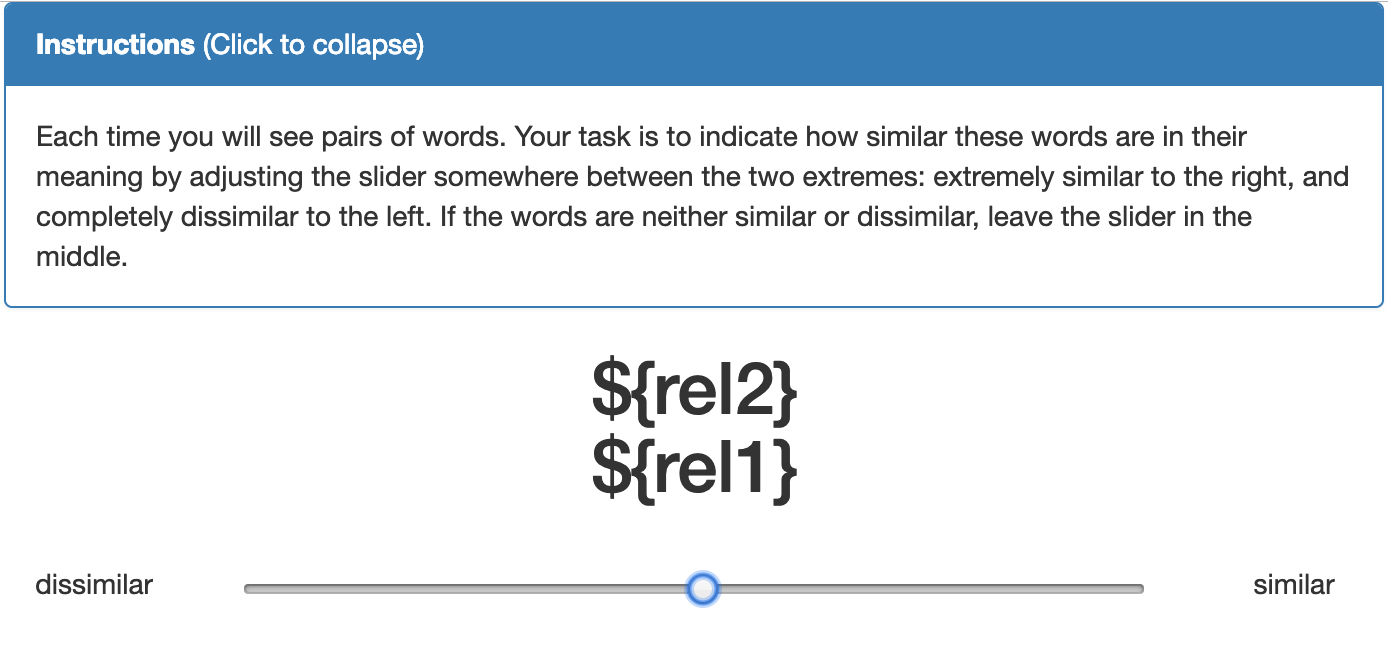
\includegraphics[width=0.85\linewidth]{studies/splu2019/figures/amt_layout_screenshot.png}
		\caption{The layout which presents the similarity judgment question.}
		\label{splu2019:fig:screenshot}
	\end{center}
\end{figure}

\clearpage
\bibliographystyle{acl_natbib}
\bibliography{studies/splu2019/references.bib}


\clearpage

\chapter{Functional/Geometric Spectrum In 
Bounding Boxes}
\chaptersource{Simon Dobnik and Mehdi Ghanimifard.}{Spatial descriptions on a functional-geometric spectrum: the location of objects.}{Preprint - Under review 2020.}

\paragraph{Abstract}
  Experimental research on spatial descriptions shows that their
  semantics are dependent on several modalities, among others (i) a
  geometric representation of space (``where'', geometric knowledge)
  and (ii) dynamic kinematic routines between objects that are related
  (``what'', functional knowledge). In this paper we examine whether
  geometric and functional bias of spatial relations is also reflected
  in large corpora of images and their corresponding descriptions. In
  particular, we examine whether the variation in object locations in the usage of a relation is a
  predictor of that relation's functional or geometric bias. Previous experimental psycho-linguistic work has examined the bias of some spatial relations, however our corpus-based computational analysis allows us to examine the bias of spatial relations and verbs beyond those that have been tested experimentally.  Our findings have also implications for
  building computational image descriptions systems as we demonstrate
  what kind of representational knowledge is required to model spatial
  relations contained in them.


\section{Introduction}\label{sc2020:sec:introduction}

The work on spatial relations such as ``the chair is to the left of
the table'' and ``the bicycle near the door'' shows that the semantics
of spatial relations is complex, drawing on several different
modalities which include among others (i) scene geometry, (ii)
functional interactions between objects, and (iii) dialogue
interaction between conversational partners. %
For example, \cite{Landau:1993aa} argue that language encodes objects
and places differently and this may be a reflection of different
cognitive processes in the visual system: ``what'' and ``where''.
Further, a number of papers \cite{CoventryEtAl:2001,Coventry:2004aa,Coventry:2005aa,Horberg:2008aa}
show experimentally that different spatial relations have different
bias in terms of functional (``what'') and geometric (``where'')
knowledge. Similarly, \cite{Landau:2016aa} argues that two classes of
spatial relations have different developmental trajectories and may be
rooted in different neural representations. \cite{Dobnik:2017ac}
argues that the bias to function and geometry of a particular relation
is contextual and task-dependent.

For this reason, computational modelling of descriptions of spatial
relations is challenging. Firstly, it requires information from each
of these modalities to be present in the dataset. For example, it is
hard to collect a large enough dataset of functional interactions
between objects and represent these interactions as computationally useful
representations. Secondly, there is a challenge of information fusion
which needs to be attuned for different words in different
contexts. Recently, deep neural networks modelling language and vision
as perceptually grounded language models have demonstrated a lot of
success \cite{Xu:2015aa,Lu:2016ab}. An interesting research question
therefore is what information such networks can capture in their
representations from the available modalities and whether such
representations correspond to the representations that have been
argued for in linguistic and psychological literature.

For example, \cite{Dobnik:2013aa,Dobnik:2014ab,dobnik-etal-2018-exploring} explore
whether functional and geometric bias can be recovered from the
information encoded in a language model, the semantic associations
encoded in the sequences of words. Language models together with word
embeddings \cite{Bengio:2003aa} are widely used to represent
linguistic meaning in computational semantics and they are based on
the premise known as the \emph{distributional hypothesis}
\cite{Firth:1957aa} that words occuring in similar contexts,
represented by other words, will have similar meanings
\cite{Turney:2010aa}. If we relate the distributional hypothesis to grounding in perception, this is because words co-occuring together will
refer to identical situations and therefore the contexts of words become
proxies for accessing the underlying situations. It follows that information encoded in
language models about spatial descriptions should encode some relevant
semantics about dynamic kinematic routines between the objects that
are related, albeit very indirectly. Hence,
\cite{Dobnik:2013aa,Dobnik:2014ab,dobnik-etal-2018-exploring} demonstrate that the
functional-geometric bias of expressions that have been tested
experimentally in \cite{CoventryEtAl:2001} is reflected in the degree
to which target and landmark objects are associated with a relation in
spatial descriptions extracted from a corpus of image
descriptions. They start with the idea that while any two (abstract)
objects can be related in geometric space, functional relations
between the objects and relation are more specific, defined by the
possible functional interaction between the objects. They demonstrate
that this is expressed in the variability and generality of the target
and landmark objects. Since a geometrically-biased spatial relation
can relate any kind of objects that can be placed in a particular
space, the objects used with such a relation will be more variable
than the objects that occur with functionally-biased relations that
also encode the nature of object interaction. They also show that
usage of descriptions of an image corpus is crucial in this task since
in a general corpus, a wider range of situations is reflected in the
word contexts that may include metaphoric usages of the spatial words
in other domains. We may consider such metaphorical usage of spatial
relations in other domains as highly functional.


The experiments based on \cite{CoventryEtAl:2001} show that spatial
relations have functional or geometric \emph{bias} which means that
both components are relevant for the semantics of a description, just
not the same degree. For example, a functionally-biased relation such
as \emph{over} is also sensitive to geometry to some extent, it
appears that a presence of a function skews the regions of
acceptability for the target object of that relation. The deviation in
geometry can be explained by the fact that under a consideration of a
functional relation different parts of the target and landmark object
will become attended \cite{Coventry:2005aa,Carlson:2006aa}. This
results in a situation where the centroids of bounding boxes of target
and landmark objects are displaced from the locations where we would
expect to find them based on the geometric constraints alone. For
example, in the case of a ``teapot over a cup'' it must be ensured
that the spout of the teapot is located in such a way so that the
liquid will be poured into a cup. In a scene described by a
description ``the toothpaste is over a toothbrush'' the shape of the
bounding boxes will be different from the previous scene as well as
the location of the attended areas. In the case of an ``apple in a
bowl'' the bowl or its contents must constrain the movement of the
apple (so that it does not fall out of the bowl) and hence locations
of apples that are outside the bounding box of the bowl are also
acceptable, for example where an apple is on the top of other
apples. These examples suggest that over all contexts of
target-landmark objects, the variation in locations of objects
represented as bounding boxes will be much higher with
functionally-biased spatial relations than geometrically-biased ones
which will be closer to the axes of the geometric space. The latter is
confirmed by the spatial templates of \cite{logan1996computational} where in
the absence of the functional knowledge, when an abstract shapes are
used as targets and landmarks, both geometric and functional relations
such as ``over'' and ``above'' give very similar axis-centred spatial
templates.  Hence, in this work, we explore whether we can detect a
difference in the variability of the target objects in relation to the
landmark objects for spatial relations of either geometric or
functional bias in terms of representations of objects as visual
features in images from a large corpus of images and descriptions and
for relations that go beyond the ones that were tested
experimentally. We expect that this variability will be the opposite
of the variability that has been previously shown for textual
data. Functional information can be recovered from the textual
information about \emph{what} objects are interacting, while geometric
information can be recovered from \emph{where} the visual features of
objects are. Hence, we expect that relations that were experimentally
found to have a functional bias will be less variable in their choice
of target and landmark objects but more variable in terms of where
these objects are in relation to the prototypical axes from the
landmark. On the other hand, relations that were experimentally found
to have a geometric bias, are expected show a higher variation in
terms of the object kinds they relate but these will be geometrically
less variable from the axes based on the landmark.

The experimental work on functional and geometric bias of spatial
relations focuses on abstract images where the type of objects, their
location and the nature of functional interaction is carefully
controlled. This gives us accurate judgements about the applicability
of descriptions but since the task focuses on abstract scenes this
gives us different judgements to those we would have hoped to have obtained in real-life
situations simply because of the perceptual and linguistic context is
different from real-life situations
\cite{Dobnik:2017ac}. %
Ideally, we would need a corpus of interactions between real objects
and their spatial descriptions that on the perceptual side would be
represented as 3-dimensional temporal model. Collecting such a corpus
on a large scale would be a very challenging endeavour, although
important work in this area has recently been done in route
instructions in a virtual environments \cite{Thomason:2019aa}. On
the other hand, there exist several large corpora of image
descriptions, e.g.  \cite{Krishna:2016aa} which contain spatial
descriptions and a large variety of interacting objects in real-life
situations. For this reason they are, in our opinion, an attractive
test-bed for examining the meaning of geometrically-biased and
functionally-biased spatial relations. The down-side of image
corpora is that the visual representations scenes are skewed, depending
on the angle and the focus/scale at which an image was taken which
means that an object such as a chair may have a different shape and
size in respect to the image from one image to another. There is
also no information about object depth and the dynamic interaction of
objects. To counter this variation in objects we will introduce some
normalisation steps. Of course, there will also be some noise in the
scene representation's we obtain but we hope this noise will be
uniform across different images and kinds of descriptions and
therefore a relative comparison of descriptions of different bias will
still give us a valid result.

Why is identification of functional and geometric bias of spatial
relations relevant? Theoretically, the experiments give us more
insights into the way spatial cognition is reflected in
language. Showing that there is a distinction between these two
classes of spatial relations on a large scale dataset of image
descriptions gives a further support to the experimental evidence that
has been obtained in carefully designed experiments. Knowing that
there are different classes of spatial relations can help us in the
task of generating image descriptions, for example in a robotic
scenario. Following our observation, in an image description task
functional relations are more informative than geometric
relations as in addition to geometric component they also say
something about the relation between the objects.\footnote{Notice,
  however, that there are tasks where geometric information may be
  more informative, for example in locating a named object in a visual
  scene when answering a question.} In a given scene a target object
can be described and related to the landmark with several spatial
relations based on geometric considerations alone. However, these
descriptions could be filtered by considering those relations that are
functionally more likely. The investigation also has implication for
end-to-end image captioning systems build with deep learning
architectures. Knowing that different spatial relations have a
different bias for visual and textual modality would allow us a better
comparison and evaluation of such systems. For example, there is a
significant discussion in the vision and language community that
end-to-end image captioning systems and visual question answering
systems are relying too much on the information from language models
\cite{Agrawal:2017aa} rather than grounding words in an image,
particularly when it comes to describing relations between
objects. Knowing that not all spatial relations are equally
geometrically spatial has important implications for evaluating such
systems: (i) it shows that provided there is a balanced dataset
reliance of a spatial relation on a language model is not necessarily
a shortcoming but rather that is in fact the dimension that determines their
meaning and there is a gradience in the way a description is grounded
in visual vs textual features; (ii) it gives us insights into how we should
build such systems in the future so that both (or even more)
modalities are appropriately represented.

This paper is organised as follows: in Section~\ref{sc2020:sec:dataset} we
describe the dataset of images and descriptions used in our studies; in
Section~\ref{sc2020:sec:dense-vectors} we describe how we represent geometric
information from image annotations for spatial relations and how such
representations can be compared for functional and geometric bias; in
Section~\ref{sc2020:sec:variation-of-dense-vectors} we introduce a more
sophisticated comparison in terms of the variation in our feature
representations for different spatial relations from a representative
representation; and we conclude in Section~\ref{sc2020:sec:conclusion}.





\section{Dataset}\label{sc2020:sec:dataset}

We base our investigations on the Visual Genome dataset
\cite{Krishna:2016aa} which is a crowd-sourced annotations
of 108,007 images. The dataset comprises several types of annotations including the
region descriptions (phrases and sentences referring to one bounding box), objects (annotated as
bounding boxes), attributes for each object annotation, and \emph{relationships} between
them (triplet of subject, predicate, object). Most object names, attributes and predicate of relationships are also mapped to WordNet synsets.
The predicates in relationships
include \emph{spatial relations} such as ``\emph{above}", ``\emph{under}", ``\emph{on}", ``\emph{in}"
but also verbs describing events such as ``\emph{holding}" and ``\emph{wearing}", or a combination of both such as ``\emph{sitting on}".

Without any data cleaning, the total number of possible forms of relation tokens is 36,550. 
Since spatial relations are multi-word expressions, we create a
dictionary of relations capturing different variations of their
syntactic form (e.g. ``to the left of'', ``on the left'', ``left'',
etc.) based on the lists of English spatial relation constructions in
\cite{Landau:1996aa} and \cite{herskovits1986language}. 
Out of 235 spatial relations, we only found 78 types.
Some variation in writing of relationships may be simply due to the
annotator shorthand notation, e.g. ``to left of''. We combine the
compound variants of spatial relations to a lower-cased single variant
in cases where we can be reasonably sure that this will not affect
their semantics in terms of functional and geometric
bias. %
Duplicate descriptions per image which are created by different
annotators are
removed, %
as well as those descriptions where the extracted spatial relations
are not used in a complete locative description involving a target
object, relation and a landmark, e.g. ``chair on left''.
At the end, we only kept those relations which have more than 30 instances in the dataset. 

In addition to spatial relations, we also added a few verbal relations which possibly have spatial content.
Including the verbs which \cite{collell2018acquiring} showed to have strong predictability of object on the y-axis. The dictionary of all relations examined in this study is given in Table~\ref{sc2020:tab:vocabulary}.

\begin{table}[hbt]
	\caption{The list of spatial relations captured and additional verbs with spatial content.}\label{sc2020:tab:vocabulary}
	\centering
	\begin{tabular}{|m{30em}|}
		\hline 
		\emph{over},
		\emph{above},
		\emph{below},
		\emph{under},
		\emph{left of},
		\emph{right of},
		\emph{on},
		\emph{in}, 
		\emph{inside},
		\emph{outside},
		\emph{far from}, 
		\emph{away from},
		\emph{next to},
		\emph{near to}, 
		\emph{across},
		\emph{at},
		\emph{with},
		\emph{beneath}, 
		\emph{underneath},
		\emph{through},
		\emph{alongside},
		\emph{against},
		\emph{off}, 
		\emph{between},
		\emph{from},
		\emph{beside}, 
		\emph{to}, 
		\emph{by}, 
		\emph{along}, 
		\emph{around},
		\emph{behind},
		\emph{bottom}, 
		\emph{top},
		\emph{front of},
		\emph{back of},
		\emph{side of}, \\
		\hline
		\emph{flying},
		\emph{kicking},
		\emph{cutting},
		\emph{catching},
		\emph{riding}, 
		\emph{seeing},
		\emph{looking}, 
		\emph{floating}, 
		\emph{finding}, 
		\emph{pulling}, 
		\emph{removing}, 
		\emph{having},
		\emph{wearing},
		\emph{containing}, 
		\emph{holding}, 
		\emph{supporting}, 
		\emph{sitting},
		\emph{touching}. \\
		\hline
	\end{tabular}
\end{table}

\section{Representing locations as dense geometric vectors}\label{sc2020:sec:dense-vectors}

Each bounding box in Visual Genome is represented with 4 numerical
values: the x-, y- coordinates relative to the image frame, the
bounding box width and
height. %
In order to compare the geometric arrangements of objects represented
as bounding boxes between different spatial relations, as well as to
compare this data with the data from spatial templates from
\cite{logan1996computational}, we convert both representations to
3-dimensional dense vectors $[x,y,d]$ where $x$ and $y$ represent
directions in the 2-dimensional space and $d$ is a Euclidean distance
between $x$ and $y$. Hence, we separate directionality (represented by
$x$ and $y$) from the distance. The intuition behind this comes from a
distinction between \emph{directionals} (``to the left of'' and
``above'') and \emph{topological relations} (``close'' and ``far'')
where the former are dependent on both directionality and distance but
the latter are only dependent on distance. The 3-dimensional vectors
(the $x$ and $y$ dimension) are inspired by vectors introduced in the
Attentional Vector Sum Model (AVS) \cite{RegierCarlson:2001}. However,
as we will describe below they are used quite differently. Rather then
modelling the attention for a particular pair of bounding boxes in the
AVS model we use them to estimate attention between all bounding boxes
that are related by a particular spatial relation. In other words, we
use them to estimate the likelihood that for a particular spatial
relation a particular location is occupied by an object. Therefore,
the representations are similar to the notion of spatial
templates. Here, other representations of bounding boxes could also be
used (see for example \cite{Sadeghi:2015aa,Nikolaus:2019aa}. We opt
for low-level features that have been experimentally shown to be
directly relevant for the (geometric) semantics of spatial relations
and which are also available in spatial templates.



\begin{figure}
	\centering
	\begin{minipage}{0.5\textwidth}
		\centering
		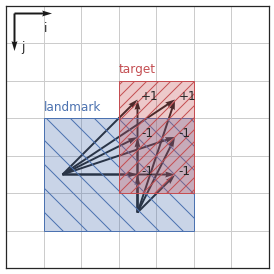
\includegraphics[width=0.75\textwidth]{studies/sc2020/figures/target_landmark_arrows.png}\\
		(a) Bounding boxes in an image
	\end{minipage}%
	\begin{minipage}{0.5\textwidth}
		\centering
		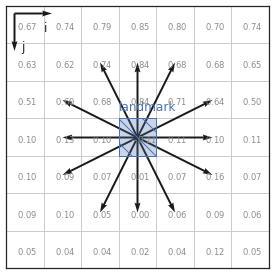
\includegraphics[width=0.75\textwidth]{studies/sc2020/figures/target_landmark_arrows_spt.png}\\
		(b) Spatial template %
	\end{minipage}%
	\caption{(a) Images are segmented to a fixed set of locations
          and relation vectors are calculated for every pair of
          locations occupied by the bounding boxes of target and
          landmark. (b) In spatial templates a vector is calculated
          for every location of the template originating in the
          location of the landmark.  } \label{sc2020:fig:bbox_vecs}
\end{figure}



We derive the dense features as follows. First, as shown in
Figure~\ref{sc2020:fig:bbox_vecs}a, we segment images into $7 \times 7$
locations. Then, for every
pair of points in the locations matrix, we define a dense vector as:

\begin{align*}
	\text{for two points on image}
	\begin{cases}
		p_1 = \langle i_1, j_1\rangle\\
		p_2 = \langle i_2, j_2\rangle
	\end{cases}, 
	\vec{u}_{p_1, p_2} = \begin{bmatrix}
	x \\
	y \\
	d 
	\end{bmatrix} = \begin{bmatrix}
	\frac{i_{2} - i_{1}}{||\overrightarrow{p_1 p_2}||_2} \\
	\frac{j_{1} - i_{2}}{||\overrightarrow{p_1 p_2}||_2} \\
	\mathtt{sgn} \cdot ||\overrightarrow{p_1 p_2}||_2
	\end{bmatrix}
\end{align*}

\noindent where $\vec{u}_{p_1, p_2}$ represents the dense geometric relation
features between two points, which $p_1$ is a point on landmark and $p_2$ is on the target, the Euclidean distance between them is $||\overrightarrow{p_1 p_2}||_2 = \sqrt{(i_{2} - i_{1})^2+(j_{2} - j_{1})^2}$, and $\mathtt{sgn}$ is a sign value which is $-1$ if $p_2$ is also a point on the landmark bounding box, otherwise $+1$.



For each relation \textsc{rel}, this gives us a collection of vectors.
For bounding boxes annotated with relations in the images of Visual Genome,
we build the collection of dense vectors of all points connecting
targets and landmarks related by each particular relation in the dataset
($V_{\textsc{rel}}^{(vg)}$). 
Formally, this
set is represented as follows:
\begin{align}
V_{\textsc{rel}}^{(vg)} = \bigg\{ \vec{u}_{p_1, p_2} \bigg\}_{\substack{
		\langle \textsc{trg},\textsc{rel}, \textsc{lnd} \rangle \in \mathrm{Images} \\
		p_1 \in \mathrm{bbox}_\textsc{lnd} \\
		p_2 \in \mathrm{bbox}_\textsc{trg}
}}
\end{align}
\noindent where $\mathrm{bbox}_\textsc{trg}$ and $\mathrm{bbox}_\textsc{lnd}$ are the collection of points in bounding boxes of target \textsc{trg} and landmark \textsc{lnd}.\footnote{For computational convenience, instead of including all possible annotations in this set, we randomly sampled a maximum of 1000 triplets from the relationship dataset.}

Similarly, we use this method on spatial templates from
\cite{logan1996computational} to build all possible dense vectors. As shown in
Figure~\ref{sc2020:fig:bbox_vecs}b, we create a dense vector originating in
the central location of the landmark and ending at every possible location
of target in the spatial template. 	
Each vector from a spatial template is associated with the acceptability score
of the target location.
\begin{align}
V^{(st)} = \bigg\{ \vec{u}_{\langle 3, 3\rangle, \langle i, j\rangle} \bigg\}_{\substack{
		i \in \{1,..,7\} \\
		j \in \{1,..,7\}
	}}, S_{\textsc{rel}} = \bigg\{ \vec{s}_{i,j} \bigg\}_{\substack{
		i \in \{1,..,7\} \\
		j \in \{1,..,7\} 
}} 
\end{align}
\noindent where $S_{\textsc{rel}}$ represents the collection of normalised acceptabilities in spatial template of the relation \textsc{rel}. 

These vectors in each collection are then projected to a single vector
representation using the following methods. 
For the collection of vectors from
a spatial template, the representative vector is the weighted sum of all possible vectors with acceptability scores:
\begin{equation}
	\vec{v}_{\textsc{rel}}^{(st)} = \sum_{\substack{
			i \in \{1,..,7\} \\
			j \in \{1,..,7\} 
		}}{s_{i,j} \cdot \vec{u}_{\langle 3, 3\rangle, \langle i, j\rangle}}
\end{equation}

\noindent For the collection of vectors from the Visual Genome bounding boxes, 
the representative vector is the expected 3-feature vector:
\begin{equation}
	\vec{v}_{\textsc{rel}}^{(vg)} = E[V_{\textsc{rel}}^{(vg)}] = \frac{1}{|V_{\textsc{rel}}^{(vg)}|}\sum_{\vec{v} \in V_{\textsc{rel}}^{(vg)}}{\vec{v}}
\end{equation}

\noindent where $|V_{\textsc{rel}}^{(vg)}|$ is the number of vectors. Adding vectors with contradicting features will cancel each other and remaining vector points at a direction with least opposite directions. More importantly, $\vec{v}_{\textsc{rel}}^{(vg)}$ resulted from bounding box annotations in visual genome is similar $\vec{v}_{\textsc{rel}}^{(st)}$ resulted from compressing the spatial templates into a three dimensional feature vectors. 


\begin{figure}
	\centering
	\begin{minipage}{\textwidth}
		\centering
		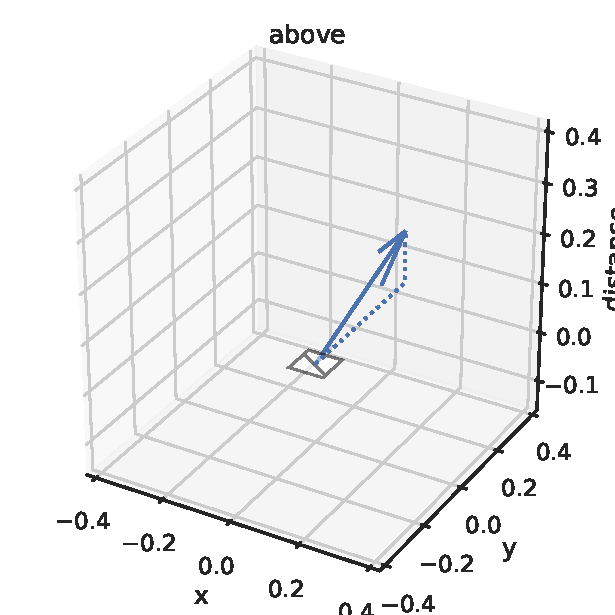
\includegraphics[width=0.2\textwidth]{studies/sc2020/figures/above_vg_features.pdf}
		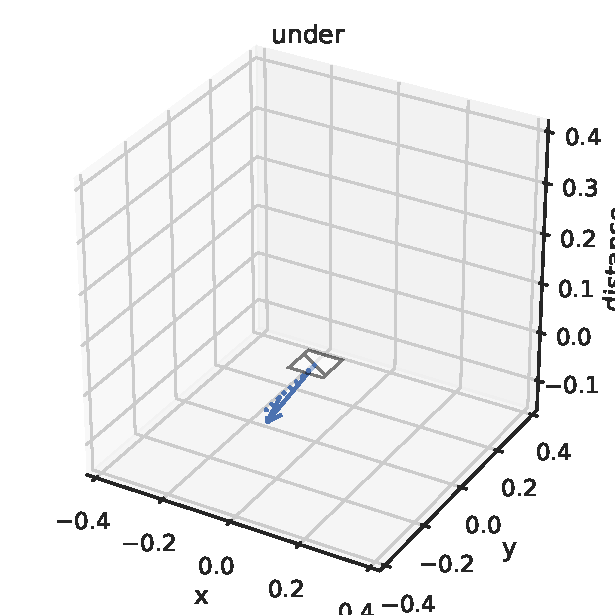
\includegraphics[width=0.2\textwidth]{studies/sc2020/figures/under_vg_features.pdf}
		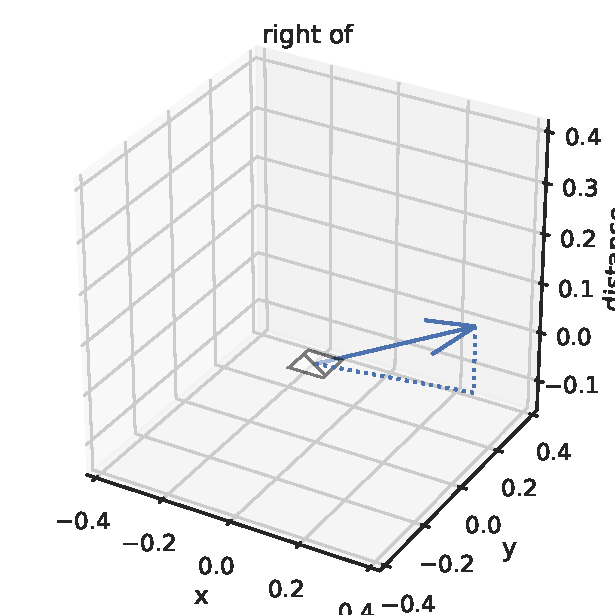
\includegraphics[width=0.2\textwidth]{studies/sc2020/figures/right_of_vg_features.pdf}
		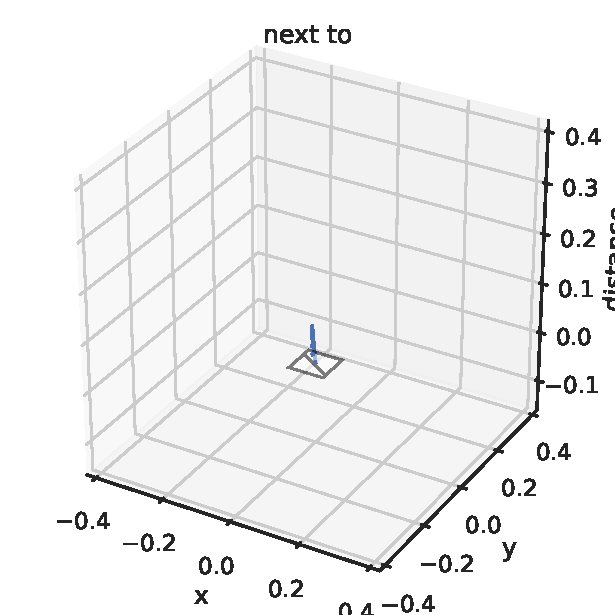
\includegraphics[width=0.2\textwidth]{studies/sc2020/figures/next_to_vg_features.pdf}
	\end{minipage}\\
	\begin{minipage}{\textwidth}
		\centering
		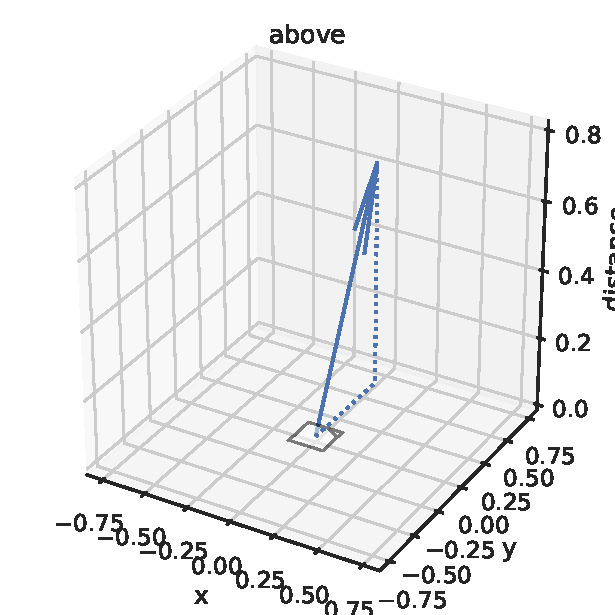
\includegraphics[width=0.2\textwidth]{studies/sc2020/figures/above_st_features.pdf}
		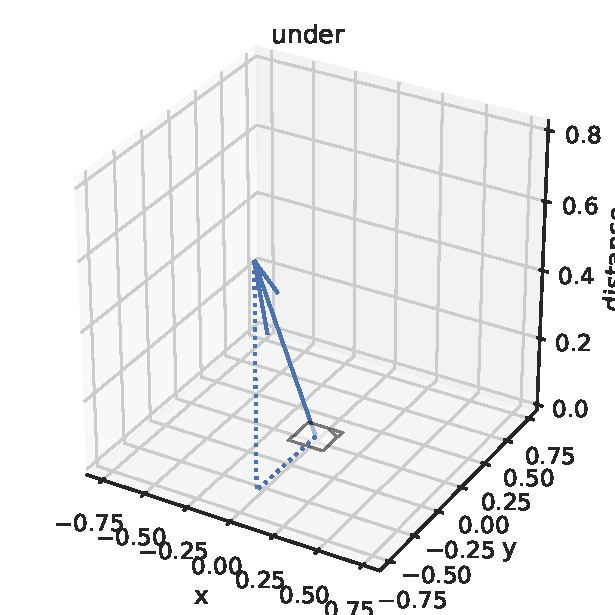
\includegraphics[width=0.2\textwidth]{studies/sc2020/figures/under_st_features.pdf}
		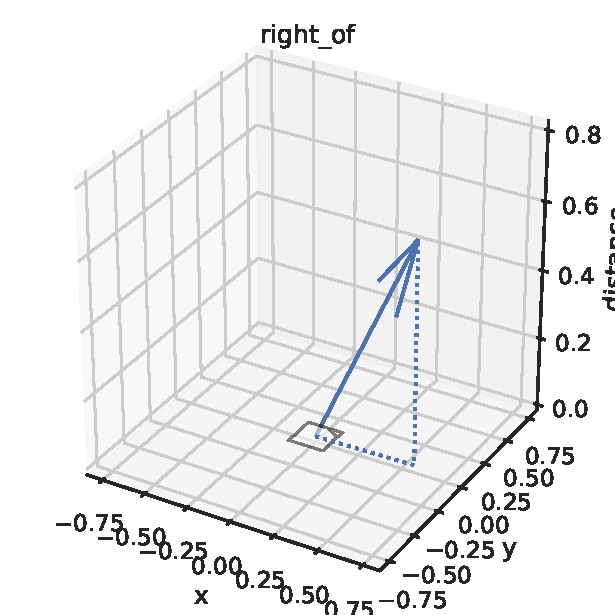
\includegraphics[width=0.2\textwidth]{studies/sc2020/figures/right_of_st_features.pdf}
		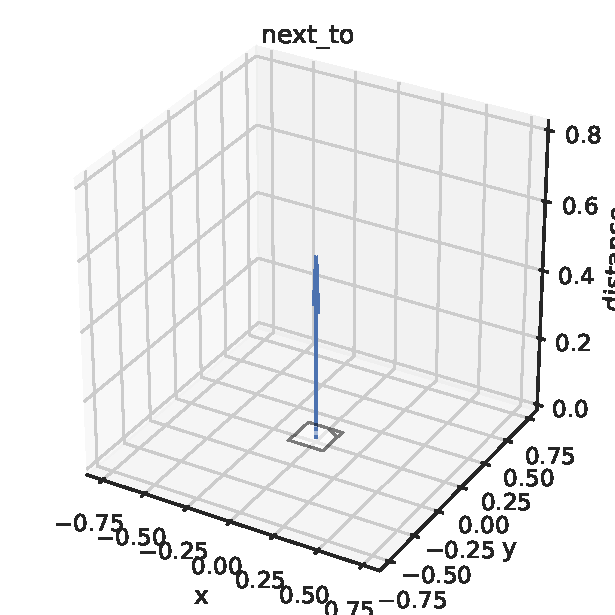
\includegraphics[width=0.2\textwidth]{studies/sc2020/figures/next_to_st_features.pdf}
	\end{minipage}\\
	\caption{Examples of $\vec{v}_{\textsc{rel}}^{(vg)}$ and  $\vec{v}_{\textsc{rel}}^{(st)}$: among the examples, x-y features are mostly similar but the scale and sign of distances are different.} \label{sc2020:fig:vg-st:samples}
\end{figure}

\begin{figure}
	\centering
	\begin{minipage}{0.6\textwidth}
		\centering
		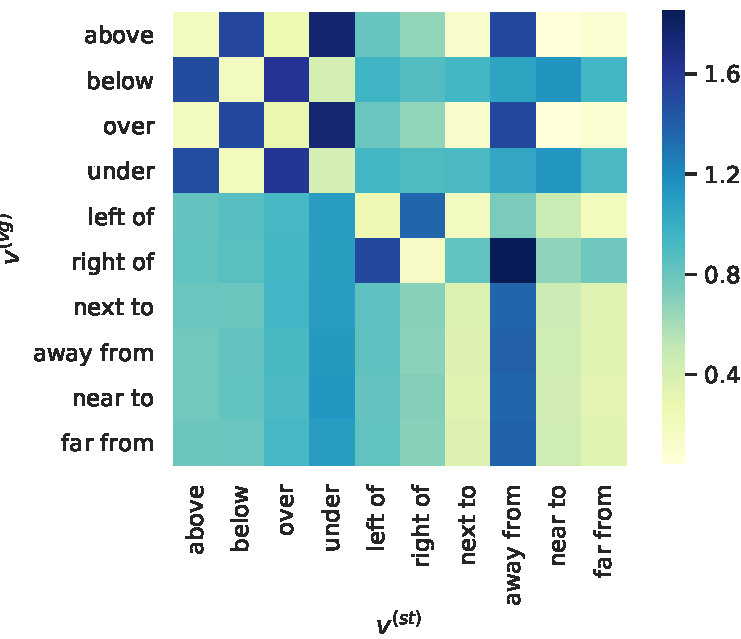
\includegraphics[width=0.85\textwidth]{studies/sc2020/figures/heatmap_distance_st_vg.pdf}
	\end{minipage}%
	\caption{A comparison of dense vector representations from images $\vec{v}_{\textsc{rel}}^{(vg)}$ and those from spatial templates $\vec{v}_{\textsc{rel}}^{(st)}$ with the cosine distance: $1-cosine(\vec{v}_{\textsc{rel}}^{(vg)}, \vec{v}_{\textsc{rel}}^{(st)})$. } \label{sc2020:fig:vg-st}
\end{figure}



To compare the projected dense vectors we have obtained from the
images with those from the spatial templates we use cosine similarity
or distance as shown in Figure~\ref{sc2020:fig:vg-st}
where the horizontal axis represents the vectors from spatial
templates $\vec{v}_{\textsc{rel}}^{(st)}$ and the vertical axis
represents the vectors from images
$\vec{v}_{\textsc{rel}}^{(vg)}$. The results indicate that the
3-dimensional vectors from the two datasets are very similar except in
the case of ``away
from''. %
Except for this case the lowest cosine distance is on the
diagonal. The results also indicate that pairs of geometrically or
functionally biased spatial relations such as ``over'' and ``above''
and ``under'' and ``below'' have similar overall directions and
distances. Projective relations have clearly defined opposites
alongside one axis but topological relations are overlapping with the
projective relations. ``next to$_{st}$'' is similar to ``next
to$_{vg}$'', ``away from$_{vg}$'', ``near to$_{vg}$'' and ``far
from$_{vg}$'' and ``away from$_{st}$'' is dissimilar to all. This has
possibly to do with the way distance is represented in images. Humans
are able to estimate distance between two focused objects not on their
actual size but the size they know from their background knowledge.

The comparison of dense vectors here indicates that similar dense
vectors are obtained from both datasets. However, it does not
distinguish functional and geometric bias of different relations. For
example, ``over$_{st}$'' is equally similar to ``over$_{vg}$'' and
``above$_{vg}$'' while we were expecting that since ``over$_{st}$'' is
used in the geometric context it will more similar to
``above$_{vg}$''. %
This is because cosine similarity/distance takes into account all
three dimensions $x$, $y$ and $z$ of the dense vectors. However, we
expect that ``over$_{st}$'' will be similar to ``over$_{vg}$'' in $y$
and $d$ dimensions but different in the $x$ dimension which
distinguishes its geometric and functional use.

In the following section we examine the 3-dimensional feature space of
the dense vectors in terms of the variation in the distribution of
features. Therefore, we need to look for a measure that captures
variation in distribution of features.


\section{Variation of features within dense vectors}\label{sc2020:sec:variation-of-dense-vectors}

We argued in Section~\ref{sc2020:sec:introduction} that we expect that
functionally-biased relations will be associated with more variable
locations of target and landmark objects as these will also be
dependent on the functional relations between individual object
pairs. In the previous section we represented the locations between
targets and landmarks as dense vectors which were then projected to
one representative vector for each spatial relation.
The degree of divergence from the representative vectors can be considered as an indication for non-geometrical use of spatial relations. 
In order to test this, for each spatial relation, we calculate a deviation of individual
target-landmark vectors $\vec{v}$ from the representative 3-dimensional dense vector $\vec{v}_{\textsc{rel}}^{(vg)}$.
As a metric of deviation we use cosine distance:

\begin{equation}\label{sc2020:eq:distances}
	Distances = \bigg\{ 1-cosine(\vec{v}_{\textsc{rel}}^{(vg)}, \vec{v}) \bigg\}_{\vec{v} \in V_{\textsc{rel}}^{(vg)}}
\end{equation}



\begin{figure}
	\centering
	\begin{minipage}{\textwidth}
		\centering
		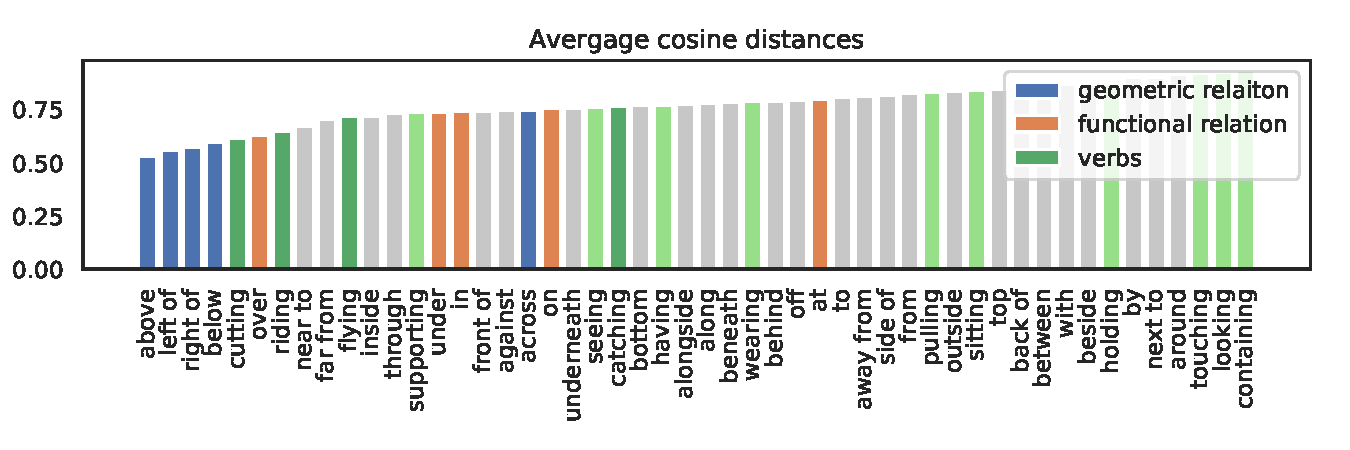
\includegraphics[width=0.8\textwidth]{studies/sc2020/figures/avg_cosine_from_bbox_fun-geo+verbs.pdf}\\ (a) \\
		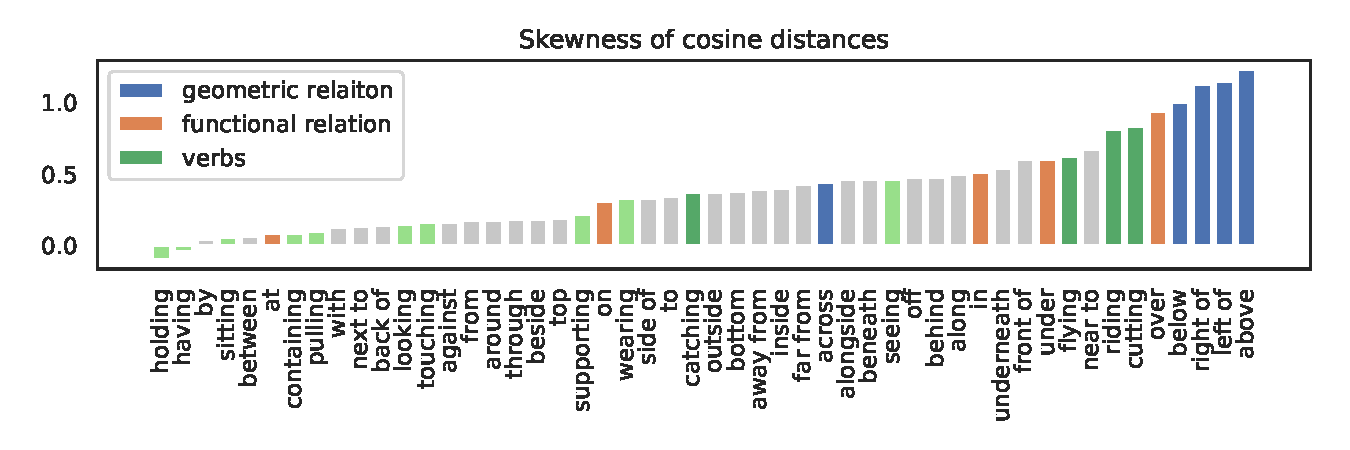
\includegraphics[width=0.8\textwidth]{studies/sc2020/figures/skewness_cosine_from_bbox_fun-geo+verbs.pdf} \\ (b)
	\end{minipage}%
	\caption{(a) The average cosine distance of dense vectors $[x, y, d]$ from the expected dense vector of each spatial relation. (b) The skewness in distribution of distances.} \label{sc2020:fig:variations}
\end{figure}





We expect that on average, cosine distances in geometrically-bias relations are closer to 0 (there is a clearer central tendency), and the overall distribution of cosine distances is positively skewed: the mode of cosine distances is close to zero while the mean and the tail of differences is skewed to the right.%
\footnote{To calculate skewness we use an implementation of the Fisher-Pearson coefficient \cite[s.2.2.24.1]{kokoska2000crc} in \href{https://docs.scipy.org/doc/scipy/reference/generated/scipy.stats.skew.html}{\texttt{scipy.stats.skew}}.}
In Figure~\ref{sc2020:fig:variations}, 
we select a set of geometrically- (blue) and functionally-biased (orange) relations as reported in
psycho-linguistic experiments and plot (a) their average cosine distances of dense vectors from their representative vector and (b) the skewness of cosine differences. %
We also include relations the bias of which has not been tested experimentally (grey) but we expect that this is demonstrated by their position in the graph between the key-points determined experimentally. Finally, we
also
include some verbs describing events and situations involving interacting objects in space that are also annotated as relationships in the Visual Genome (green), e.g. ``boy, feeds, giraffe''. We are particularly interested in the verbs that are reported in Collel et al. \cite{collell2018acquiring} for which the location of the (target) object is most strongly predictable from the $y$ dimension (``flying'', ``kicking'', ``cutting'', ``catching'' and ``riding'') (dark green in Figure~\ref{sc2020:fig:variations}) and those for which the $y$ dimensions is the least predictable in respect to the location of the object (``see'', ``float'', ``finding'', ``pulled'' and ``removes'') (light green) listed in their Table 3, p.6770. However, here \cite{collell2018acquiring} do not consider the $x$-dimension which may be a relevant dimension for the verbs in the picture.
A quick comparison of the two lists gives an impression that the
former contains descriptions of events involving object relations that
more strongly grounded in the image representations (e.g. ``riding'')
and are therefore similar to geometrically-biased spatial relations,
while the second list contains descriptions of events that are less
strongly grounded in the image representations (e.g. ``sees'') and
would require a simulation of dynamic kinematic routines between the
objects which makes them similar to functionally-biased spatial
relations.

Examining the average cosine distances from the representation vector
of each spatial relation in Figure~\ref{sc2020:fig:variations}a we can see
that relations that have been identified as geometrically-biased
(blue) tend to have a lower average cosine distance from the
representation's dense vector than those that have been identified as
functionally-biased (orange). The same tends also to be the case for
verbs identified in \cite{collell2018acquiring} for which the objects
are more dependent on the $y$ (dark green) compared to verbs for which
the objects are less dependent on the $y$ dimension (light
green). Note that in this comparison a deviation of the entire
3-dimensional vector $[x, y, d]$ was taken into account and therefore
a deviation can be in any of these dimensions. Examining the skewness
of cosine distances from the representation vector of each spatial
relation in Figure~\ref{sc2020:fig:variations}b we can see that
geometrically-biased verbs and verbs that are more strongly grounded
show a tendency towards a higher skewness of distribution, they are
more biased towards the representational vectors. Overall, the results
indicate support for our hypothesis in Section\ref{sc2020:sec:introduction}
that bounding boxes are predictors of the functional and geometric
bias as well as they indicate that the same bias is also present in
verbal descriptions of scenes.

\begin{figure}
	\centering
	\begin{minipage}{0.5\textwidth}
		\centering
		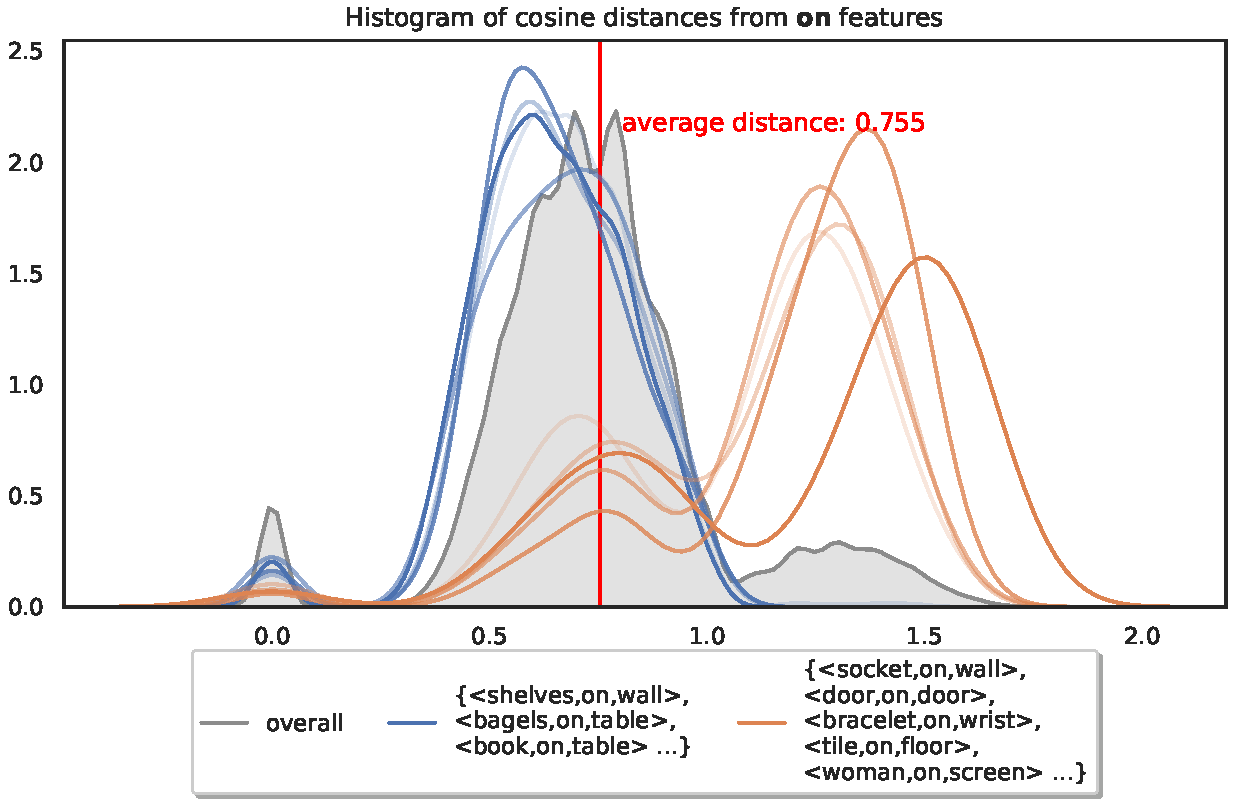
\includegraphics[width=0.85\textwidth]{studies/sc2020/figures/on_variations_what.pdf}
	\end{minipage}%
	\begin{minipage}{0.5\textwidth}
		\centering
		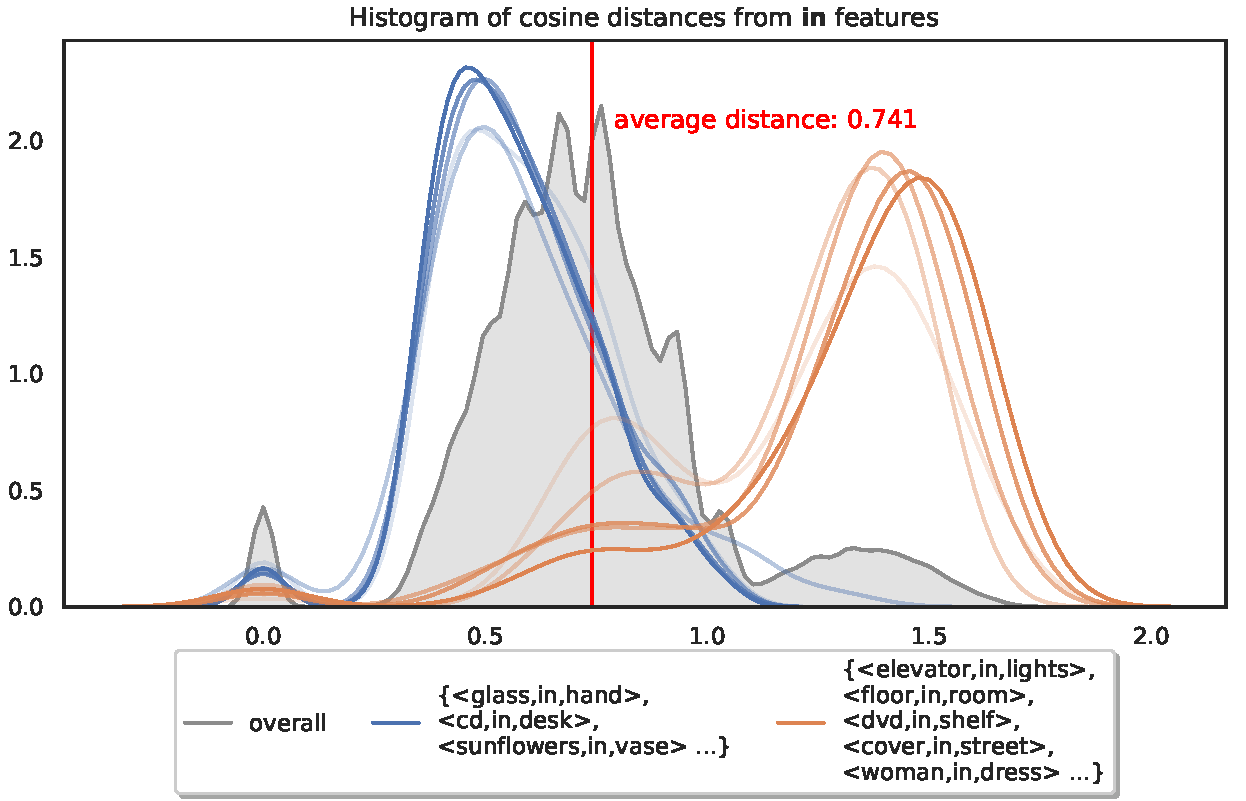
\includegraphics[width=0.85\textwidth]{studies/sc2020/figures/in_variations_what.pdf}
	\end{minipage}\\
	\begin{minipage}{0.5\textwidth}
		\centering
		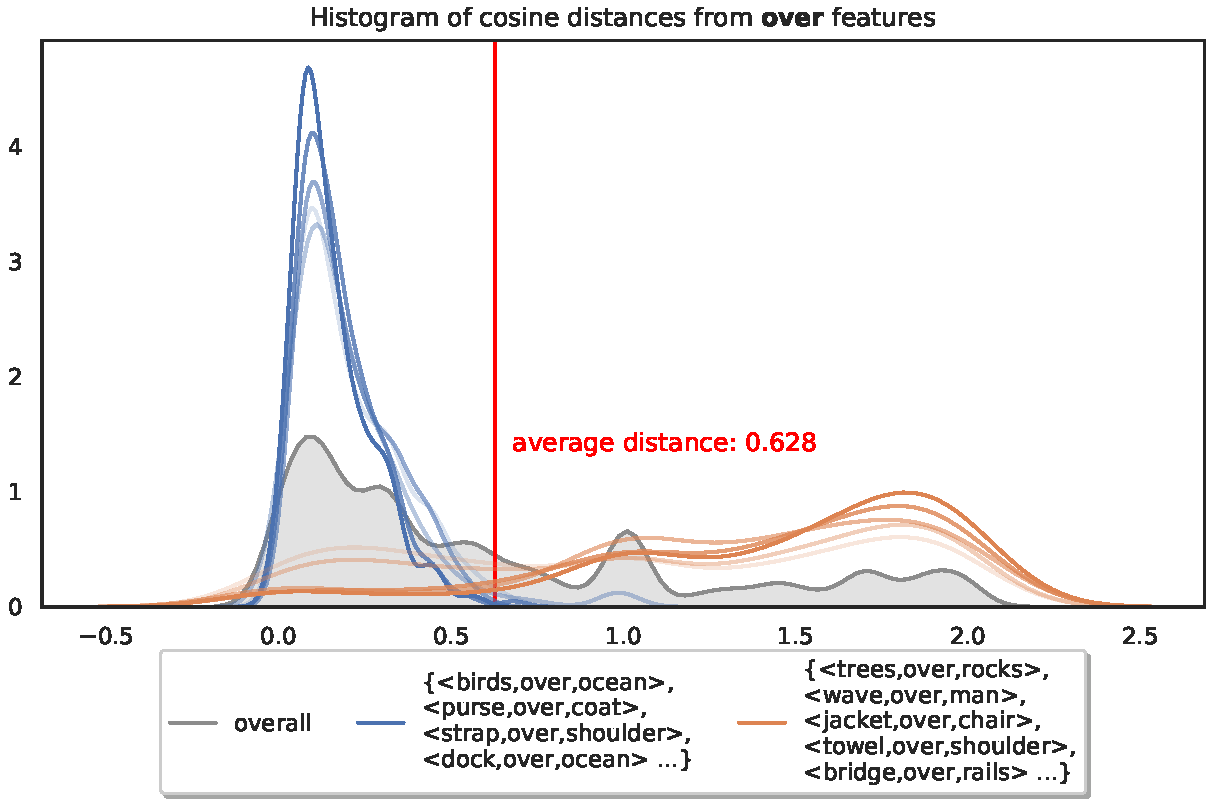
\includegraphics[width=0.85\textwidth]{studies/sc2020/figures/over_variations_what.pdf}
	\end{minipage}%
	\begin{minipage}{0.5\textwidth}
		\centering
		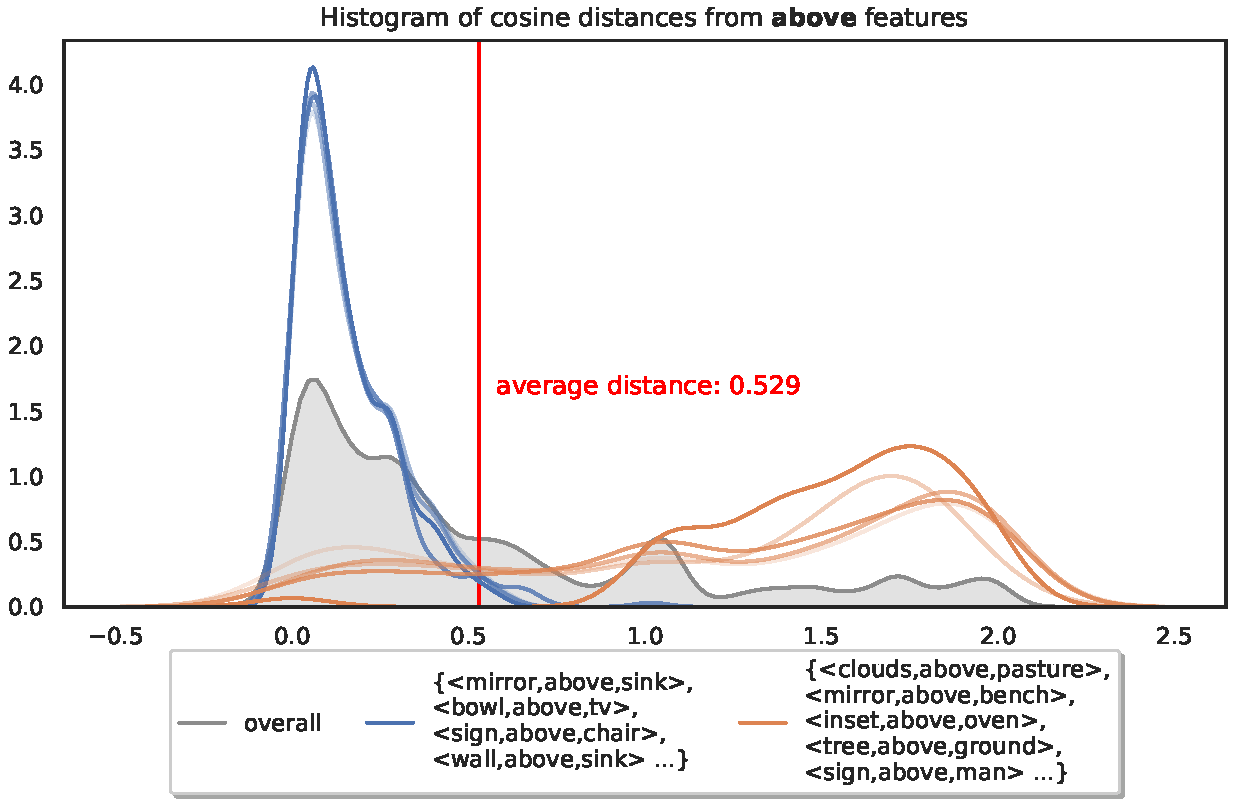
\includegraphics[width=0.85\textwidth]{studies/sc2020/figures/above_variations_what.pdf}
	\end{minipage}\\
	\begin{minipage}{0.5\textwidth}
		\centering
		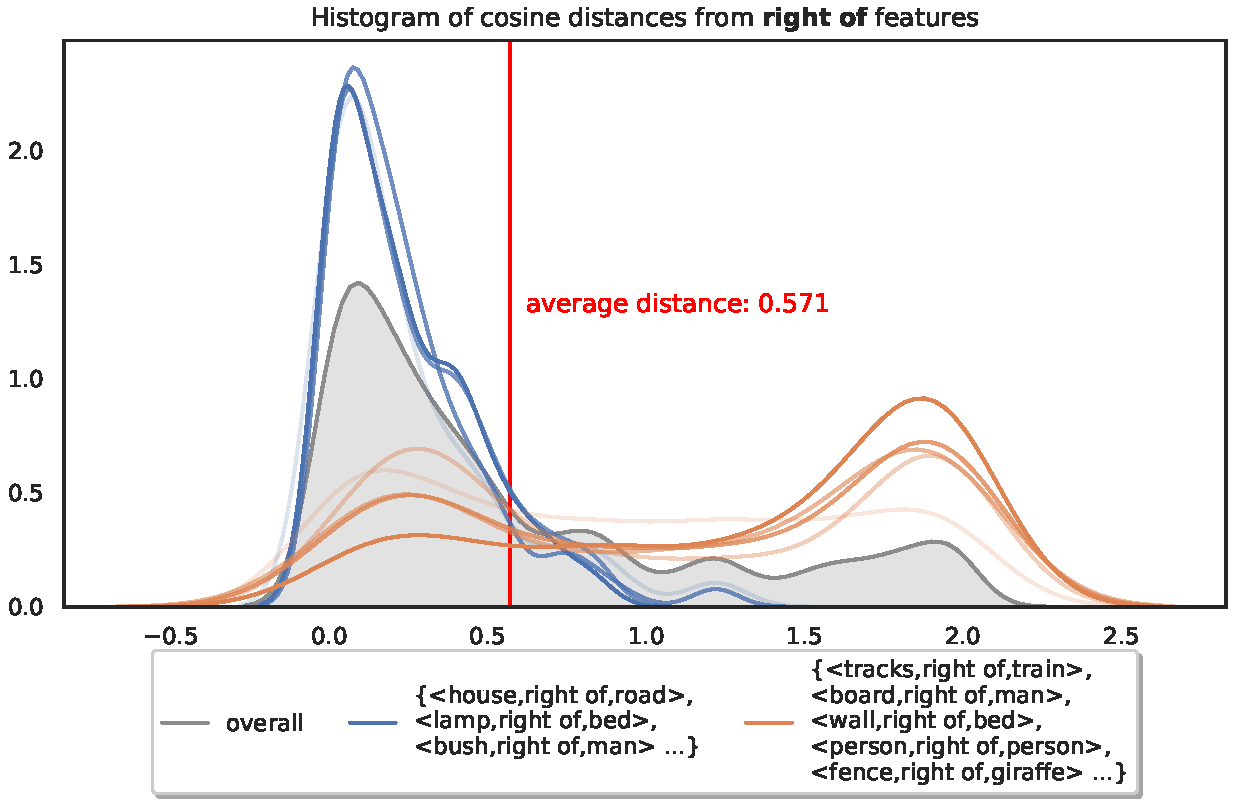
\includegraphics[width=0.85\textwidth]{studies/sc2020/figures/right_of_variations_what.pdf}
	\end{minipage}%
	\begin{minipage}{0.5\textwidth}
		\centering
		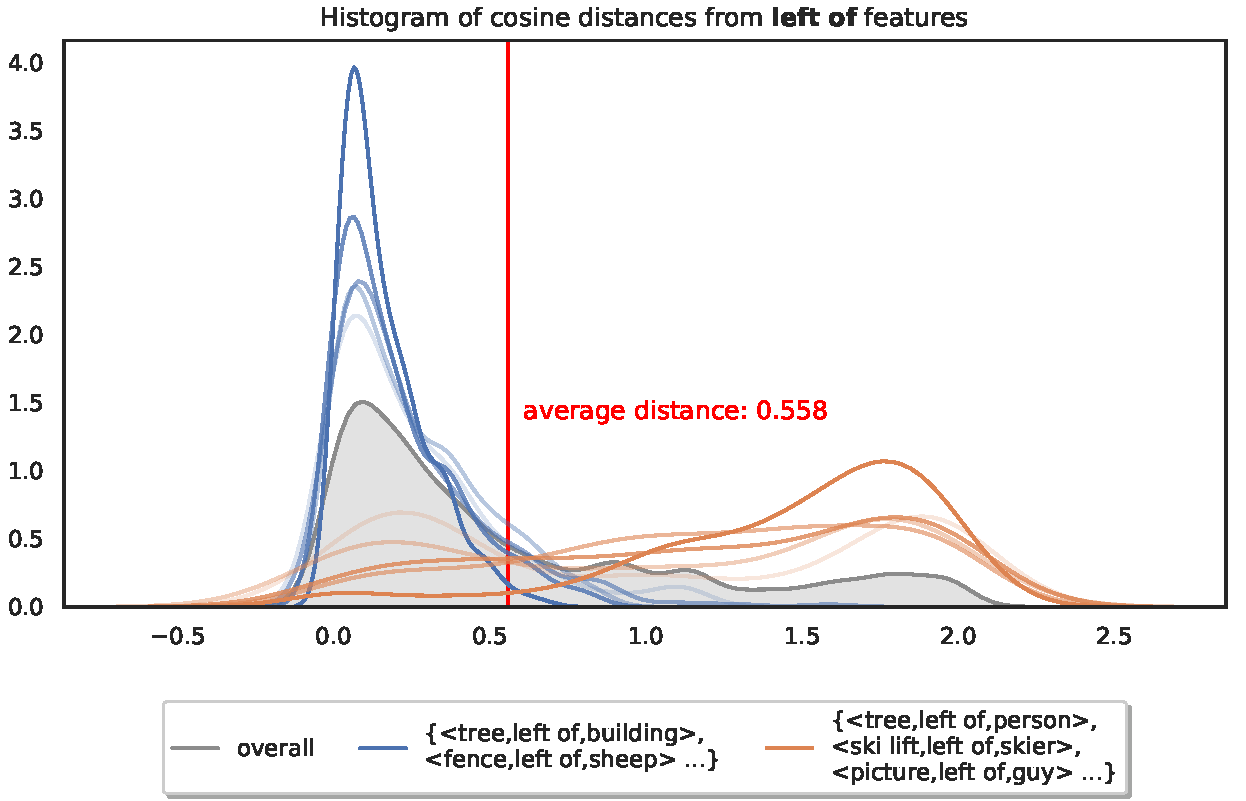
\includegraphics[width=0.85\textwidth]{studies/sc2020/figures/left_of_variations_what.pdf}
	\end{minipage}%
	\caption{Using the KDE method we plot a histogram of cosine distances of individual examples from the representational vector of each relation which shows skewness to zero for geometrically-biased usages of relations. For the projective relations ``right of'' and ``left of'' the examples with landmarks with tendency for enforcing intrinsic frame of reference (animate objects, objects with clearly defined front and back) are negatively skewed which represents maximum cosine distance. %
        }\label{sc2020:fig:what_hist}
\end{figure}




In Figure~\ref{sc2020:fig:what_hist} we examine the histograms of deviations
from the representational vectors of ``on'', ``in'', ``over'',
``above'', ``right of'' and ``left of''.  To plot these histograms we
use Kernel Density Estimation (KDE)\footnote{We use an implementation based on  \href{https://docs.scipy.org/doc/scipy/reference/generated/scipy.stats.gaussian_kde.html}{\texttt{scipy.stats.gaussian\_kde}}} \cite{scott2015multivariate} which
indicates the density of samples in the range of [0, 2] of the cosine
distance (Equation~\ref{sc2020:eq:distances}). We also give examples of
target-landmark pairs which have the highest (orange) and the lowest
(blue) average distances from the representational vectors. These
examples indicate that functionally biased relations (``on'', ``in''
and ``over'') can be and are used in contexts where the geometric
constraint is also satisfied and this is represented in the image
while they can also be used in the contexts where there is a deviation
from the geometric constraint, just as predicted by experiments in
\cite{CoventryEtAl:2001}. Interestingly, among the cases that show
high deviation from the representational vectors we also find examples
that are typically considered to involve more complex geometric
conceptualisation, for example ``bracelet on wrist'', ``woman in
dress'', ``trees over rocks''. However, the relations that we consider
to be geometrically-biased we also find examples of high deviation
from the representational vectors. The examples for ``above'' seem to
to correspond to usages where there is an element of
covering/protection that has been argued to be the functional
component of ``over'': e.g. ``clouds above/over pasture'' and ``mirror
above/over bench'' or cases that require complex geometric
conceptualisation of the scene ``tree above ground''.\footnote{It
  could be argued that these cases require functional representation
  since one needs to know how to geometrically conceptualise the scene
  involving that particular pair of objects in order the geometric
  relation can be established.} We are intrigued by the examples that
deviate from the representational vectors for ``left of'' and ``right
of''. They frequently contain animate beings (people) or objects with
clear orientation. Our assumption is that these examples are a
reflection of changes of the perspective from the relative frame of
reference of the observer of the image to the intrinsic frame of
reference of the landmark.



\begin{figure}
	\centering
	\begin{minipage}{0.1\textwidth}
		\centering
		above
	\end{minipage}%
	\begin{minipage}{0.3\textwidth}
		\centering
		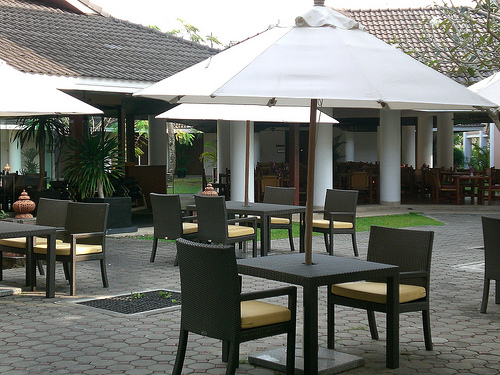
\includegraphics[width=0.7\textwidth]{studies/sc2020/figures/2407611_umbrella_above_table.jpg}
	\end{minipage}%
	\begin{minipage}{0.6\textwidth}
		\centering
		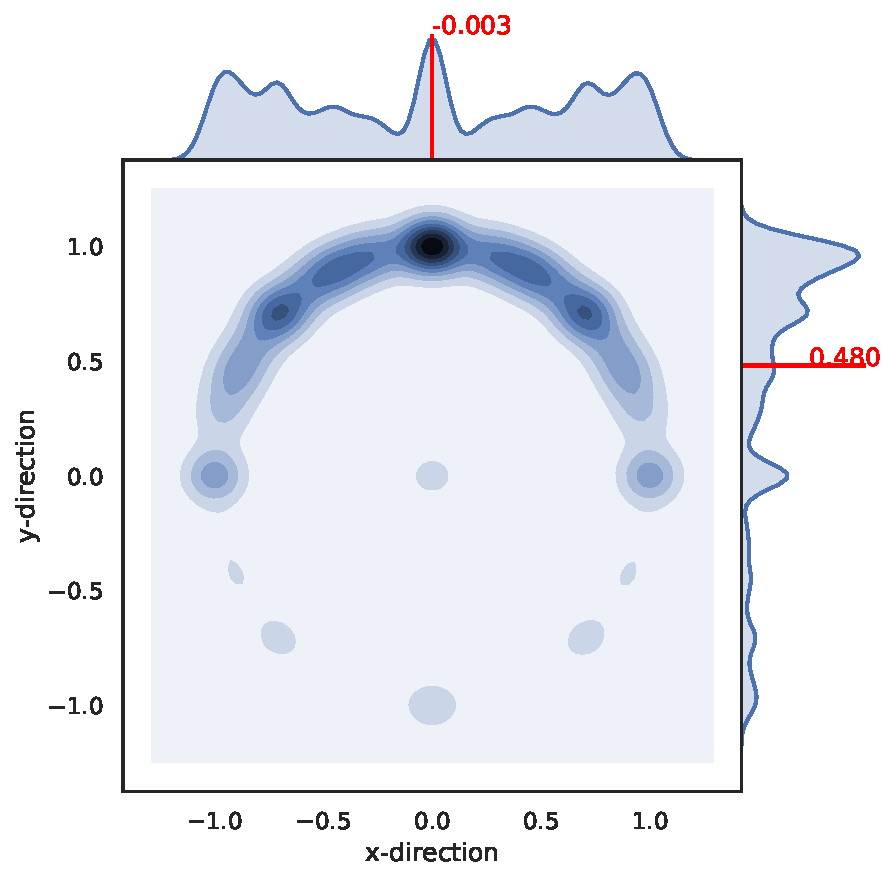
\includegraphics[width=0.45\textwidth]{studies/sc2020/figures/above_xy.pdf}
		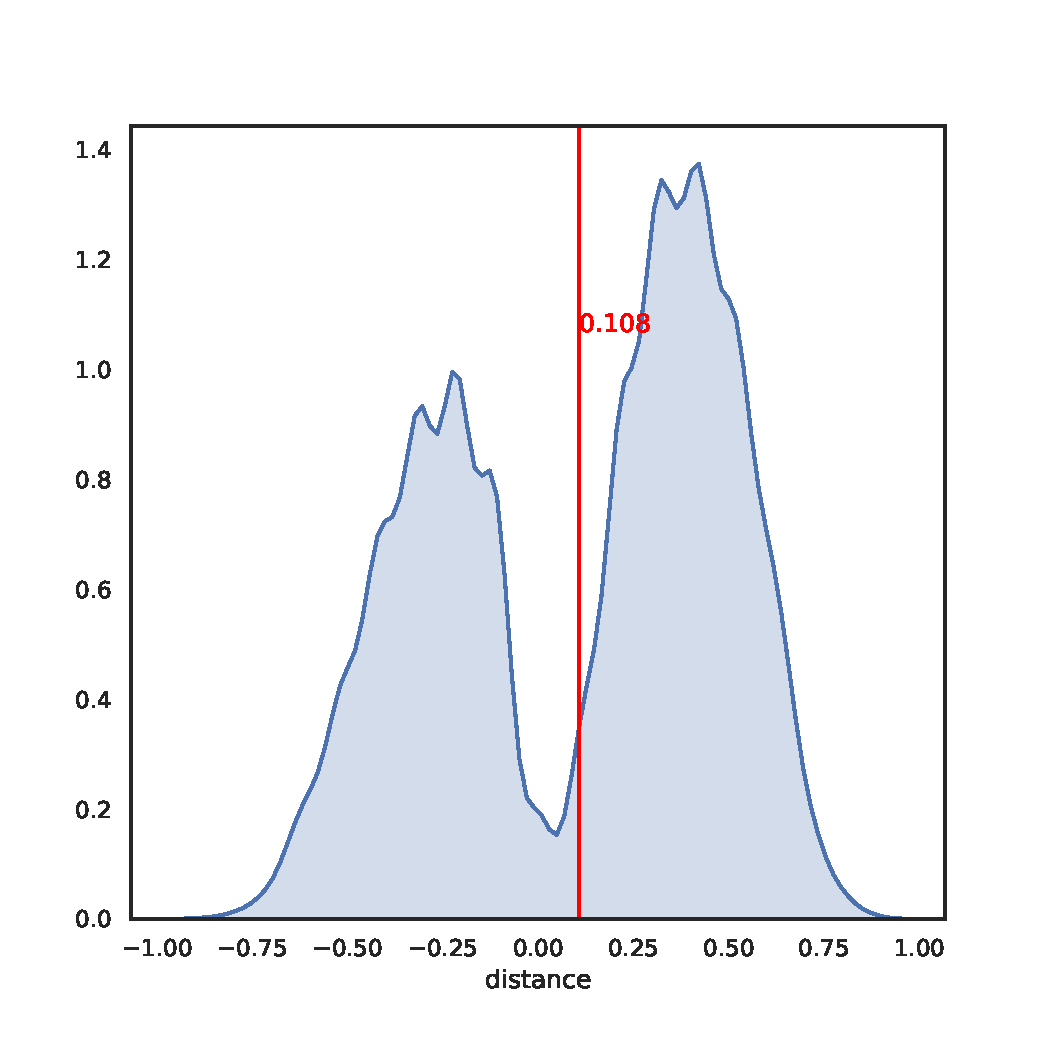
\includegraphics[width=0.45\textwidth]{studies/sc2020/figures/above_d.pdf}
	\end{minipage}\\%
	\begin{minipage}{0.1\textwidth}
		\centering
		over
	\end{minipage}%
	\begin{minipage}{0.3\textwidth}
		\centering
		\includegraphics[width=0.7\textwidth]{studies/sc2020/figures/2370756_umbrella_over_woman.jpg}
	\end{minipage}%
	\begin{minipage}{0.6\textwidth}
		\centering
		\includegraphics[width=0.45\textwidth]{studies/sc2020/figures/over_xy.pdf}
		\includegraphics[width=0.45\textwidth]{studies/sc2020/figures/over_d.pdf}
	\end{minipage}\\%
	\begin{minipage}{0.1\textwidth}
		\centering
		cutting
	\end{minipage}%
	\begin{minipage}{0.3\textwidth}
		\centering
		\includegraphics[width=0.7\textwidth]{studies/sc2020/figures/2384609_man_cutting_cake.jpg}
	\end{minipage}%
	\begin{minipage}{0.6\textwidth}
		\centering
		\includegraphics[width=0.45\textwidth]{studies/sc2020/figures/cutting_xy.pdf}
		\includegraphics[width=0.45\textwidth]{studies/sc2020/figures/cutting_d.pdf}
	\end{minipage}%
	\caption{The individual features of dense vectors $[x,y,d]$ have different distributions for each relation.} \label{sc2020:fig:features_dist} %
\end{figure}




As stated earlier, the dense vector representations including their
cosine distances aggregate three features $[x,y,d]$ and therefore the
previous comparisons do not take into account the role of each
individual feature for spatial relations.  In
Figure~\ref{sc2020:fig:features_dist} we plot the distribution of all
features over all vectors of $V_{\textsc{rel}}^{(vg)}$ for some
individual relations.\footnote{These relations were found to be
  strongly dependent on the $y$ feature in \cite{collell2018acquiring}
  who did not investigate the contribution of other features.}  The
individual histograms for the $x$ (centre top), $y$ (centre right) and
$d$ feature (on the right side) indicate the density of their values
and the mixture density graph for $x, y$ (centre) shows how these
features interact.
This graph demonstrates that ``over'' and ``cutting'' have more
freedom of variation in the $x$ dimension as well as the negative $y$
dimension (which indicates overlap of objects) than ``above''. As
discussed earlier, there is also considerable overlap between all
three graphs which is due to the fact that functionally-biased
relations are also used in situations when geometric constraints
are satisfied. While ``cutting'' is more similar to ``over'' than
``above'' in terms of the $xy$ dimensions, it has a different distance
histogram with far fewer overlapping cases.





\section{Conclusion}\label{sc2020:sec:conclusion}

In this paper we have demonstrated and discussed how the functional and
geometric bias of spatial relations can be identified from geometric
annotations of objects as bounding boxes connected by spatial
relations in a corpus of images and associated descriptions. The
bounding boxes are converted to 3-dimensional dense vectors that
contain information about the $x$, $y$ and $d$ dimension. These
vectors can be then converged to a single representational vector for
each spatial relation. Vectors from different relations can then be
compared with cosine similarity. To increase the granularity of
comparison we examine how individual examples of annotated situations
diverge from the representational vectors and what are the
distributions of these divergences, also at the level of individual
features. Our results indicate that functional and geometric bias of
spatial relations can be identified from the geometric spatial
information corpus of images and descriptions and also that this
distinction can be carried over to verbs describing situations
involving objects. In terms of semantics of spatial relations our
study shows that to a certain degree information that was previously
determined experimentally can be uncovered from a large corpus of
image descriptions and for a large number of relations including
verbs. Practically, such information is extremely useful for building
end-to-end deep neural models of image captioning as it demonstrates
what kind of representations are relevant for different kinds of
descriptions which has also been the focus of our other
studies. Another question that we find relevant to explore in our
future work is the observation that the context in which the dataset was
created may have a general bias on the degree to which function and
geometry is considered to be relevant. For example, is the goal of the
image description task to describe \emph{what} is happening with the
objects or to locate \emph{where} the objects are. Finally, different
classes of verbs would also deserve a more focused study.





\clearpage
\bibliographystyle{acl_natbib}
\bibliography{studies/sc2020/references.bib}

\clearpage

\chapter{Evaluating Generation Of Spatial Descriptions With Adaptive Attention}
\chaptersource{Mehdi Ghanimifard and Simon Dobnik.}{Evaluating Generation of Spatial Descriptions with Adaptive Attention.}{In European Conference on Computer Vision, pp. 153-161. Springer, Cham, 2018.}

\paragraph{Abstract}
  We examine and evaluate adaptive attention \cite{lu2017knowing} (which balances the focus on visual features and focus on textual features) in generating image captions in end-to-end neural networks, in particular how adaptive attention is informative for generating spatial relations.
  We show that the model generates spatial relations more on the basis of textual rather than visual features and therefore confirm the previous observations that the learned visual features are missing information about geometric relations between objects.

\section{Introduction}

End-to-end neural networks are commonly used in image description tasks
\cite{vinyals2015show,xu2015show,lu2017knowing}. Typically, a pre-trained
convolutional neural network is used as an encoder which produces visual
features, and a neural language model is used as a decoder that generates
descriptions of scenes. The underlying idea in this
\emph{representation learning} scenario \cite{bengio2013representation} is that
hidden features are learned from the observable data with minimum engineering
effort of background knowledge. For example in word sequence generation only
some general properties of a sequence structure \cite{sutskever2014sequence}
are given to the learner while the learner learns from the observed data what
word to choose in a sequence together with a representation of features. Recent
models such as \cite{xu2015show,lu2017knowing} also add to the neural language
model a model of visual attention over visual features which is inspired by the
attention mechanism for alignment in neural machine translation \cite{bahdanau2014neural}.
It may be argued that the attention mechanism introduces modularity to
representation learning in the sense of \emph{inception modules}
\cite{szegedy2015going} and \emph{neural module networks}
\cite{andreas2016neural}. The visual attention is intended to detect the
salient features of the image and align them with words predicted by the
decoder. In particular, it creates a sum of the weighted final visual features at
different regions of an image:
\begin{equation}\label{sivl2018:eq:spatialatt}
\bm{c}_t = \sum_{i=1}^k \bm{\alpha}_{ti} \bm{v}_{i}
\end{equation}
where at time $t$, $\bm{c}_t$ represents the pooled visual features, $i$
corresponds to $k$ different regions of image, $\bm{v}_{i}$ is the visual
representation of a particular region, and $\bm{\alpha}_{ti}$ represent the
amount of attention on the specific region of the image. This representation
provides the features for grounding the prediction of next word:
\begin{equation}\label{sivl2018:eq:grounding}
log Pr(w_{t+1} = y_{t+1} | w_{1:t} = y_{1:t}, I=v_{1:k}) \approx f(y_{1:t}, c_{t})
\end{equation}
where $f$ represents the end-to-end neural network for approximating the
prediction of the next word in sentence.

However, not all words in natural language descriptions are directly grounded
in visual features which leads \cite{lu2017knowing} to extend the attention
model \cite{xu2015show} with an adaptive attention mechanism which learns to
balance between the contribution of the visual signal and the language signal
when generating a sequence of words.
\begin{equation}\label{sivl2018:eq:adaptive-attention}
\hat{\bm{c}}_t = \beta_t \bm{s}_t + (1-\beta_t) \bm{c}_t
\end{equation}
where at time $t$, $\hat{\bm{c}}_t$ is a combined representation of language
features and visual features in addition to $\bm{c}_t$ of the visual features
from Equation~\ref{sivl2018:eq:grounding}. $\bm{s}_t$ is obtained from the memory state
of the language model, and $\beta_t$ ranging between $[0, 1]$ is the adaptive
attention balancing the combination of vision and language features.

The performance of the image captioning systems when evaluated on the
acceptability of the generated descriptions is impressive. However, in order to
evaluate the success of learning we also need to understand better what the
system has learned especially because good overall results may be due to the
dataset artefacts or the system is simply learning from one modality only,
ignoring the other \cite{agrawal2018don}. Understanding the representations
that have been learned also gives us an insight into building better systems
for image captioning, especially since we do not have a clear understanding of
the features in the domain. An example of work in this area is \cite{liu2017attention} which evaluates
visual attention on objects localisation. \cite{shekhar2017foil_acl} developed
the FOIL dataset as a diagnostic tool to investigate if models look at images
in caption generation. In \cite{shekhar2017vision} they examine the FOIL diagnostic for different
parts-of-speech and conclude that the state of the art models can locate
objects but their language models do not perform well on other parts-of-speech.

The current paper focuses on generation of spatial descriptions, in particular
locative expressions such as ``the chair to the left of the sofa'' or ``people
close to the statue in the square''. Spatial relations relate a target
(``people'') and landmark objects (``the statue'') with a spatial relation
(``close to''). They depend on several contextual sources of information such as
scene geometry (``where'' objects are in relation to each other), properties
or function of objects and their interaction (``what'' is related) as well as
the interaction between conversational participants \cite{herskovits1986language,Landau:1993aa,Regier:1996,Coventry:2004aa,Dobnik:2017af}.
The features that are relevant in computational modelling of spatial language
are difficult to determine simply by manually considering individual examples and they are normally
identified through experimental work. The representation learning models are
therefore particularly suited for their computational modelling.

However, the end-to-end vision and language models with attention are
implemented in a way to recognise objects and localise their area in an image
\cite{ba2014multiple,mnih2014recurrent}. To generate spatial relations,
\cite{ramisa2015combining} propose a combination of visual representations from
convolutional neural networks and manually designed geometric representation of
targets and landmarks. On quick examination, the representation of attention
over images as in \cite{xu2015show} gives an impression that attention captures
both ``what'' and ``where'', especially because the attention graphs resemble
\emph{spatial templates} \cite{logan1996computational}. However,
\cite{kelleher2017not} argue that due to the design properties of image
captioning networks, attention does not capture ``where'' as these models are
built to identify objects but not geometric relations between them which
they examine at the level of qualitative evaluation of
attention on spatial relations.

In this paper we quantitatively evaluate the model of adaptive attention of
\cite{lu2017knowing} in predicting spatial relations in image descriptions.
The resources used in our evaluation are described in
Section~\ref{sivl2018:sec:resources}. In Section~\ref{sivl2018:sec:detection} we examine the
grounding of different parts-of-speech in visual and textual part of attention.
Furthermore, in Section~\ref{sivl2018:sec:grounding} we investigate the attention on
spatial relations, targets and landmarks. We conclude by providing the possible
directions for future studies and improvements.

\section{Datasets and Pre-trained Models}\label{sivl2018:sec:resources}

As a part of their implementation \cite{lu2017knowing} provide two different
pre-trained image captioning models: Flickr30K \cite{young2014image} and
MS-COCO \cite{lin2014microsoft}.\footnote{ \url{https://filebox.ece.vt.edu/~jiasenlu/codeRelease/AdaptiveAttention}.}
We base our experiments on spatial descriptions of 40,736 images in the MS-COCO test corpus.

\section{Visual Attention and Word Categories}\label{sivl2018:sec:detection}

\paragraph{Hypothesis}

Our hypothesis is that visual attention in the end-to-end image captioning
systems works as an object detector similar to
\cite{ba2014multiple,mnih2014recurrent}.
Therefore, we expect the adaptive attention to prefer to attend to visual
features rather than the language model features when predicting categories of
words found in noun phrases that refer to objects, in particular head nouns.
We expect that both scores will be reversed:
more predictable words by the language model in the blind test receive less
visual attention.

\paragraph{Method}

We use the pre-trained model of adaptive attention
\footnote{\url{https://filebox.ece.vt.edu/~jiasenlu/codeRelease/AdaptiveAttention/model/COCO/coco_challenge/model_id1_34.t7}}
to generate a description for each of the 40,736 images in the MS-COCO-2014
test. All the attention values are logged ($\alpha, \beta$). We apply universal
part-of-speech tagger from NLTK \cite{bird2009natural} on the generated
sentences and report the average visual attentions on each part-of-speech.
We match our results with results on the degree of predictability of each
part-of-speech from the language model without looking at the image from
the blind test of \cite{shekhar2017vision}.
Note that we do not investigate the overall quality of the model on the test
set (this has already been evaluated by its authors)
but what kind of attention this model gives to vision and language features
used to generate a word of each category.
The evaluaiton code:  \\
\url{https://github.com/GU-CLASP/eccv18-sivl-attention}

\paragraph{Results}
Table~\ref{sivl2018:tab:pos} indicates that the highest degree of visual attentions is
on numbers (NUM), nouns (NOUN), adjectives (ADJ) and determiners (DET)
respectively. Pronouns (PRON) and particles (PRT) receive the lowest degree of
visual attention. Verbs (VERB) and adverbs (ADV) are placed in the middle of
this sorted list. Spatial relations which are mainly annotated as
prepositions/adpositions (ADP) receive the second lowest visual attention,
higher only than pronouns (PRON) and particles (PRT). Our results are
different from the accuracy scores of detecting mismatch descriptions in the
FOIL classification task \cite{shekhar2017vision}.
For example, the model assigns predicts the mismatch on ADJ easier than
mismatch on ADV. As hypothesised, the part-of-speech that make up noun phrases
receive the highest visual attention (and the lowest language model attention).
The results also indicate that the text is never generated by a single
attention alone but a combination of visual and language model attentions.
Since some spatial relations are often annotated as adjectives (e.g.
``front''), a more detailed comparison on spatial terms is required.

\begin{table} %
    \centering
    \begin{tabular}{|l|r|c|l|}
      \hline
        \textbf{POS} & \textbf{Count} & $\textbf{Mean} \pm \textbf{std}$ & \textbf{Blind test} %
        \\
        \hline
        NUM 	& 1882  	& $0.81 \pm 0.08$ & -
        \\
        NOUN	& 134332	& $0.78 \pm 0.12$ & 0.23
        \\
        ADJ 	& 23670 	& $0.77 \pm 0.14$ & 0.76
        \\
        DET 	& 96641 	& $0.73 \pm 0.12$ & -
        \\
        VERB	& 38381 	& $0.70 \pm 0.11$ & 0.57
        \\
        CONJ	& 6755  	& $0.70 \pm 0.13$ & -
        \\
        ADV 	& 184   	& $0.69 \pm 0.12$ & 0.18
        \\
        ADP 	& 64332 	& $0.62 \pm 0.15$ & 0.54
        \\
        PRON	& 2347  	& $0.53 \pm 0.14$ & -
        \\
        PRT 	& 6462  	& $0.52 \pm 0.21$ & -
      \\
      \hline
    \end{tabular}
	\vspace{0.5em}
    \caption{The average visual attention $(1-\beta)$ for predicting words on
	each part-of-speech. The scores from the blind test indicate the accuracy
	of detecting a mismatch description in the FOIL-classification task
	\cite{shekhar2017vision}.}\label{sivl2018:tab:pos}
\end{table}

\section{Visual Attention when Grounding Spatial Descriptions}\label{sivl2018:sec:grounding}

In generation of a sequence of words that make up a spatial description, which type of features or evidence is taken into consideration by the model as the description unfolds?

\paragraph{Hypothesis}
In Section~\ref{sivl2018:sec:detection}, we argued that the generation of spatial relations (prepositions/adpositions) is less dependent on visual features compared to noun phrases due to the fact that the learned visual features are used for object recognition and not recognition of geometric spatial relations between objects. Moreover, the visual clues that would predict the choice of spatial relation are not in one specific region of an image; this is dependent on the location of the target, the landmark and the configuration of the environment as a whole. Therefore, our hypothesis is that when generating spatial relations the visual attention is more spread over possible regions rather than being focused on a specific object.

\paragraph{Method}
The corpus tagged with POS from the previous section was used. In order to
examine the attention on spatial relations, a list of keywords from
\cite{herskovits1986language,Landau:1993aa} was used to identify them, provided that
they have a sufficient frequency in the corpus. The average adaptive visual
attention for each word can be compared with the scores in Table~\ref{sivl2018:tab:pos}
for different parts-of-speech. In each sentence, the nouns before the spatial
relation and the nouns after the spatial relations are taken as the most likely
targets and landmarks respectively.
The average adaptive visual attention on targets, landmarks and
and spatial relations is recorded.

\paragraph{Results}

In Table~\ref{sivl2018:tab:spatialkey} we report for each spatial relation and its
targets and landmarks the average adaptive visual attention. The adaptive
attentions for triplets are comparable with the figures for each part-of-speech
in Table~\ref{sivl2018:tab:pos}. In the current table, the variance of visual attentions
is reported with the $max-min$ measure which is the difference between maximum
and minimum attentions on a 7x7 plane representing the visual regions in the
model. Lower values indicate either a low attention or a wider spread of attended area, hence less visual
focus. Higher values indicate that there there is more visual focus. For each
spatial relation, the triplets must be compared with each other. In all cases,
our hypothesis is confirmed: (1) the adaptive visual attention is lower on
predicting spatial relations which means that they receive overall less visual
attention, (2) with the exception of ``under'', the difference between maximum
and minimum visual attentions are lower with spatial relations which means that
the attention is spread more over the 7x7 plane. Figure~\ref{sivl2018:fig:images}
shows a visualisation of these results for ``under'' and ``over''. The results
also show that landmarks in most cases receive less visual attention in
comparison to targets. This indicates that after providing a target and a
spatial relation, the landmark is more predictable from the language model (for
a similar observation see \cite{dobnik-etal-2018-exploring}).

\begin{table}[ht]
    \centering
    \begin{tabular}{|l|c|c|}
      \hline
        Descriptions
        & Average $(1-\beta_t)$
        & Average $(max(\hat{\alpha_t})-min(\hat{\alpha_t}))$ \\
        \textbf{Spatial Relations}
        &\textbf{TRG, REL, LND }
        &\textbf{TRG, REL, LND} \\
        \hline
        under
        & $0.84$, $\textbf{0.73}$, $ 0.79$ & 0.0252, 0.0151, \textbf{0.0139} \\
        front
        & $0.83$, $\textbf{0.70}$, $ 0.82$ & 0.0230, \textbf{0.0136}, 0.0154 \\
        next
        & $0.82$, $\textbf{0.68}$, $0.78$ & 0.0224, \textbf{0.0136}, 0.0138 \\
        back
        & $0.85$, $\textbf{0.68}$, $0.84$ & 0.0332, \textbf{0.0186}, 0.0272 \\
        in
        & $0.82$, $\textbf{0.68}$, $0.77$ & 0.0250, \textbf{0.0149}, 0.0164 \\
        on
        & $0.81$, $\textbf{0.68}$, $0.75$ & 0.0249, \textbf{0.0154}, 0.0175 \\
        near
        & $0.80$, $\textbf{0.67}$, $0.76$ & 0.0221, \textbf{0.0133}, 0.0169 \\
        over
        & $0.77$, $\textbf{0.62}$, $0.75$ & 0.0205, \textbf{0.0133}, 0.0193 \\
        above
        & $0.73$, $\textbf{0.64}$, $0.77$ & 0.0167, \textbf{0.0134}, 0.0231 \\
        \hline
    \end{tabular}
	\vspace{0.5em}
    \caption{
	The average score of adaptive visual attention for target (TRG) relation
	(REL) landmark (LND) triplets per each relation in the first column and
	the average difference between the highest and the lowest value of visual
	attention for the same items in the second column.}
	\label{sivl2018:tab:spatialkey}
\end{table}


\begin{figure}[ht]%
    \centering
    \includegraphics[width=0.4\linewidth]{studies/sivl2018/figures/over-adaptive.pdf}
    \includegraphics[width=0.4\linewidth]{studies/sivl2018/figures/under-adaptive.pdf}
    \vspace{0.5em}
    \caption{
   	Each square in a box in the first row represents an averaged attention for a location in the 7x7 grid over all $n$ generated samples $(\hat{\alpha})$. The colours fade to white with lower values. The bottom graphs show their average over the entire plane, indicating the degree of adaptive visual attention $(1-\beta)$, also reported in Table~\ref{sivl2018:tab:spatialkey}.}\label{sivl2018:fig:images}
\end{figure}

\section{Discussion and Conclusion}

In this paper we explored to what degree adaptive attention is grounding
spatial relations. We have shown that adaptive visual attention is more
important for grounding objects but less important for grounding spatial
relations which are not directly represented with visual features.
As a result the visual attention is diffused over a larger space. The
cause for a wider attended area can be due to high degree of
noise in visual features or lack of evidence for visual grounding.

This is a clear shortcoming of the image captioning model, as it is not able to discriminate
spatial relations on the basis of geometric relations between the objects,
for example between relations such as ``left'' and ``right''. The future work
on generating image descriptions therefore requires models where visual geometry between
objects is explicitly represented as in \cite{Coventry:2005aa}. The study also
shows that when generating spatial relations, a significant part of the
information is predicted by the language model. This is not necessarily a
disadvantage. The success of distributional semantics shows that language
models with word embeddings can learn a surprising amount of semantic
information without access to visual grounding. As mentioned in the
introduction, spatial relations do not depend only on geometric arrangement of
objects but also functional properties of objects. For example,
\cite{dobnik-etal-2018-exploring} demonstrate that neural language models encode such
functional information about objects when predicting spatial relations. Since,
each spatial relation has different degree of functional and geometric bias
\cite{Coventry:2004aa}, the adaptive attention considering visual features and
textual features is also reflective of this aspect.

Models for explaining language model predictions such as \cite{park2016attentive} are also related to this study and its future work.

Our study focused on the adaptive attention in \cite{lu2017knowing} which
explicitly models attention as a focus on visual and language features.
However, further investigations of other types of models of attention could be
made and this will be the focus of our future work. We expect that different
models of attention will behave similarly in terms of attending visual features
on spatial relations
because the way visual features are represented: they favour detection of
objects and not their relative geometric arrangement. Our future work we will
therefore focus on how to formulate a model to be able to learn such geometric
information in an end-to-end fashion.
Methodologies such as \cite{ribeiro2016should} and \cite{selvaraju2017grad}
which investigate the degree of effectiveness of features without attention
are also possible directions of the future studies.

\section{Acknowledgements}
We are also grateful to the anonymous reviewers for their helpful comments on our earlier draft. The research reported in this paper was supported by a grant from the Swedish Research Council (VR project 2014-39) for the establishment of the Centre for Linguistic Theory and Studies in Probability (CLASP) at the University of Gothenburg.


\section{Appendix: Supplementary Material}

\begin{figure}[ht!]
	\centering
	\includegraphics[width=0.4\columnwidth]{studies/sivl2018/figures/above-adaptive.pdf}
	\includegraphics[width=0.4\columnwidth]{studies/sivl2018/figures/at-adaptive.pdf}
\end{figure}
\begin{figure}[ht!]
	\centering
	\includegraphics[width=0.4\columnwidth]{studies/sivl2018/figures/back-adaptive.pdf}
	\includegraphics[width=0.4\columnwidth]{studies/sivl2018/figures/behind-adaptive.pdf}
\end{figure}
\begin{figure}[ht!]
	\centering
	\includegraphics[width=0.4\columnwidth]{studies/sivl2018/figures/by-adaptive.pdf}
	\includegraphics[width=0.4\columnwidth]{studies/sivl2018/figures/down-adaptive.pdf}
\end{figure}
\begin{figure}[ht!]
	\centering
	\includegraphics[width=0.4\columnwidth]{studies/sivl2018/figures/front-adaptive.pdf}
	\includegraphics[width=0.4\columnwidth]{studies/sivl2018/figures/in-adaptive.pdf}
\end{figure}
\begin{figure}[ht!]
	\centering
	\includegraphics[width=0.4\columnwidth]{studies/sivl2018/figures/inside-adaptive.pdf}
	\includegraphics[width=0.4\columnwidth]{studies/sivl2018/figures/near-adaptive.pdf}
\end{figure}
\begin{figure}[ht!]
	\centering
	\includegraphics[width=0.4\columnwidth]{studies/sivl2018/figures/next-adaptive.pdf}
	\includegraphics[width=0.4\columnwidth]{studies/sivl2018/figures/on-adaptive.pdf}
\end{figure}
\begin{figure}[ht!]
	\centering
	\includegraphics[width=0.4\columnwidth]{studies/sivl2018/figures/over-adaptive.pdf}
	\includegraphics[width=0.4\columnwidth]{studies/sivl2018/figures/under-adaptive.pdf}
\end{figure}


\clearpage
\bibliographystyle{acl_natbib}
\bibliography{studies/sivl2018/references.bib}

\clearpage

\chapter{Generating Descriptions With Top-Down Spatial Knowledge}
\chaptersource{Mehdi Ghanimifard and  Simon Dobnik.}{What Goes Into A Word: Generating Image Descriptions With Top-Down Spatial Knowledge.}{In Proceedings of the 12th International Conference on Natural Language Generation. 2019.}

\paragraph{Abstract}
Generating grounded image descriptions requires associating linguistic units with their corresponding visual clues.
A common method is to train a decoder language model with attention mechanism over convolutional visual features. %
Attention weights align %
the stratified visual features %
arranged by their location with tokens, most commonly words, in the target description.
However, %
words such as %
spatial relations (e.g. \emph{next~to} and \emph{under}) are not directly referring to geometric arrangements of pixels but to complex geometric and conceptual representations.
The aim of this paper is to evaluate what representations facilitate generating image descriptions with spatial relations and lead to better grounded language generation. %
In particular, we investigate the contribution of four different representational modalities in generating relational referring expressions:
(i) (pre-trained) convolutional visual features, (ii) spatial attention over visual features, (iii) top-down geometric relational knowledge between objects, and (iv) world knowledge captured by contextual embeddings in language models.


\section{Introduction}\label{inlg2019:sec:introduction}

Spatial recognition and reasoning are essential bases for visual understanding.
Automatically generating descriptions of scenes
involves both recognising objects and their spatial configuration.
This project follows up on recent attempts to improve language
generation and understanding %
in terms of using spatial modules in the fusion of vision and
language
\cite{xu2015show,johnson2016densecap,lu2017knowing,hu2017modeling,anderson2018bottom} (see also %
Section~\ref{inlg2019:sec:related_works}).

Generating spatial descriptions is an important part of the image
description task which requires
several types of knowledge obtained from different modalities: %
 (i) invariant visual clues for object identification,
 (ii) geometric configuration of the scene representing relations between objects relative to the size of the environment %
 (iii) object-specific functional relations that capture interaction between them and are formed by our knowledge of the world %
 for example \emph{an umbrella is over a man} is true if the referring
umbrella serves its function, protecting the man from the rain \cite{coventry2001interplay}, and
 (iv) for projective relations (e.g. ``to the left of'' and ``above'') but not topological relations (e.g. ``close'' and ``at''), the frame of reference which can be influenced from other modalities such as scene attention and dialogue interaction %
 \cite{Dobnik:2015aa}.
 Work in cognitive psychology \cite{logan1994spatial,logan1995linguistic} argues that while object identification may be pre-attentive, identification of spatial relations is not and is accomplished by a top-down mechanisms of attention after the objects have been identified. It is also the case that we do not identify all possible relations between objects but only those that are attended by such top-down mechanisms considering different kinds of high-level knowledge.

Experiments on training neural recurrent %
language models in a bottom-up fashion from data\footnote{
  A bottom-up learning acquires higher level representations from examples of local features rather than using an external procedure to extract them. %
  See also Section~\ref{inlg2019:sec:related_works}.
}
demonstrated that spatial relations are frequently not learned to be grounded in visual inputs
\cite{lu2017knowing,tanti2018quantifying,ghanimifard2018knowing}
which has been attributed
to the design choices of these models that primarily focus on
identification of objects \cite{kelleher2017what}.
Therefore, targeted integration of different modalities is required to
capture the properties from (i) to (iv).  
We can do this top-down	%
\cite{anderson2018bottom,hu2017modeling,liu2017attention}.  
However,
it is not immediately obvious \emph{what} kind of top-down spatial
knowledge will benefit the bottom-up models most. Therefore, in this
paper we investigate the integration of different kind of top-down
spatial knowledge beyond object localisation represented as features with the bottom-up neural
language model.


















The paper is organised as follows.
In Section~\ref{inlg2019:sec:generating_locative_expressions}, we discuss how
spatial descriptions are constructed and what components are required
to generate descriptions. In Section~\ref{inlg2019:sec:neural_net_design}, the
neural networks' design is explained. In Section~\ref{inlg2019:sec:dataset}, we
explain what dataset is used for this study, what pre-processing
was applied on it and how the models are trained. Then the experiments and evaluation results are
presented in Section~\ref{inlg2019:sec:evaluation}. The related work in relation to our methods and findings is discussed %
in Section~\ref{inlg2019:sec:related_works}. %
The conclusion is
given in Section~\ref{inlg2019:sec:conclusion}.


\section{Generating Spatial Descriptions} %
\label{inlg2019:sec:generating_locative_expressions}

When describing a scene, there are several ways to construct spatial
descriptions referring to objects and places and their relation with
each other.  A spatial description has three parts: a \textsc{target}
and a \textsc{landmark} referring to objects or places and a
\textsc{relation} denoting the location of the target in relation to
the landmark \cite{logan1996computational}.\footnote{Sometimes these are also known as \emph{referent} and \emph{relatum} \cite{Miller-JohnsonLaird:1976}, \emph{figure} and \emph{ground} \cite{Talmy:1983} or \emph{the located object} and \emph{the reference object} \cite{herskovits1986language,Gapp:1994:BasicMeanings,Dobnik:2009dz}.} These are in the example in
Figure~\ref{inlg2019:fig:data_example} as follows:

\noindent There~is~$\underbracket{a~teddy~bear}_{\textsc{Target}}~\underbracket{partially~under}_{\textsc{Relation}}~\underbracket{a~go~cart}_{\textsc{Landmark}}$.
\begin{figure}[tb]
	\begin{minipage}{\columnwidth}
	\centering
	\includegraphics[width=0.4\columnwidth]{studies/inlg2019/figures/2318741.pdf}\\
	$\langle$ ``{\color{red} teddy bear}", ``partially under", ``{\color{blue} go cart}"$\rangle$
	\caption{$\langle$\textsc{target}, \textsc{relation}, \textsc{landmark}$\rangle$ annotation of bounding boxes in VisualGenome 2318741\protect\footnote{\citet{vg2318741}: CC BY-SA 2.0.} }
	\label{inlg2019:fig:data_example}
	\end{minipage}
\end{figure}

\noindent Therefore generating such description requires
(a) identification of objects and their locations:
the target is what we want to describe
and the landmark is what we will relate the target to;
the salience of the landmark is important for the hearer.
(b) Grounding of the relation in geometric space:
the spatial relation is expressed relative to the landmark which
grounds a 3-dimensional coordinate system; furthermore, for projective
relations, the coordinate system is aligned with the orientation of
the external viewpoint which determines the frame of
reference \cite{Maillat:2003}. (Viewpoint may also be the landmark object itself in which
case the coordinate system is oriented in the same way as the
landmark).
(c) Grounding in function:
a spatial relation may be selected also based on the functional
properties between target and landmark objects,
e.g. the difference between ``\textit{the teapot is over the
cup}" and ``\textit{the teapot is above the cup}" \cite{coventry2001interplay}.

Generating spatial descriptions requires knowing the intended target object
and how we want to convey its location to the listener.  The bottom-up
approach in image captioning is focused on learning the salience of
objects and events to generate captions expressed in the dataset (e.g. \citet{xu2015show}).  The combination of bottom-up and
top-down approaches for generating descriptions %
use modularisation in order to improve the generation of descriptions of different kind (e.g. \citet{you2016image}). %
However, as we have seen in the preceding discussion, the generation of
spatial descriptions requires a highly specific geometric knowledge.
How is this knowledge approximated by the bottom-up models?  To what
degree can we integrate this knowledge with the top-down models?  In this
paper, we investigate these questions in a language generation task by comparing
different variations of included top-down spatial knowledge.
More specifically, for each image, we generate a description
for every pair of objects that are localised in the image.
We consider a variety of top-down spatial knowledge representations about objects
as inputs to the model:
(a) explicit object localisation and extraction of visual features;
(b) explicit identification of the target-landmark by specifying their order in the feature vector;
and (c) explicit geometric representation of objects in a 2D image. %
We investigate the contribution of each of these sets of features to generation of image descriptions. %




\section{Neural Network Design}\label{inlg2019:sec:neural_net_design}

Our method is to add step-by-step modules and configurations to the network %
providing different kind of top-down knowledge in Section~\ref{inlg2019:sec:generating_locative_expressions} and investigating the performance of such configurations.
There are several design choices with small effects on the performance but costly in terms of parameter size \cite{tanti2018put}.
Therefore, if there is no research question related to that choice, we take the simplest choice as reported in the previous work such as \cite{lu2017knowing,anderson2018bottom}.
We
use the following configurations: %

\begin{enumerate}[nosep]
	\item Simple bottom-up encoder-decoder; %
	\item Bottom-up object localisation with attention;
	\item Top-down object annotated localisation;
	\item Top-down target and landmark assignment;
	\item Two methods of top-down representation of geometric features ($\bm{s}$-features).
\end{enumerate}
These five %
configurations %
give us 10 variations of the model design as shown in Table~\ref{inlg2019:tab:models}. %
\begin{table*}[htb]
	\centering
	\scriptsize
	\begin{tabular}{|l|l|l|l|l|}
		\hline
		 Model name & Regions Of Interest & \textsc{target}-\textsc{landmark} & $\bm{s}$-features & Architecture \\
		\hline
		$simple$     & - & - & - & Figure~\ref{inlg2019:fig:architectures}a \\
		\hline
		$bu49$       & Bottom-up ($7\mathrm{x}7$ grid) & Bottom-up attention & - & Figure~\ref{inlg2019:fig:architectures}b \\
		$bu49+mask$  & Bottom-up ($7\mathrm{x}7$ grid) & Bottom-up attention & Multi-hot 98 & Figure~\ref{inlg2019:fig:architectures}c \\
		$bu49+VisKE$ & Bottom-up ($7\mathrm{x}7$ grid) & Bottom-up attention & Dense 11 & Figure~\ref{inlg2019:fig:architectures}c \\
		\hline
		$td$         & Top-down (2 bbox) & Bottom-up attention & -    & Figure~\ref{inlg2019:fig:architectures}d \\
		$td+mask$    & Top-down (2 bbox) & Bottom-up attention & Multi-hot 98  & Figure~\ref{inlg2019:fig:architectures}e \\
		$td+VisKE$   & Top-down (2 bbox) & Bottom-up attention & Dense 11 & Figure~\ref{inlg2019:fig:architectures}e \\
		\hline
		$td~order$         & Top-down (2 bbox) & Top-down assign. & - & Figure~\ref{inlg2019:fig:architectures}d \\
		$td~order+mask$    & Top-down (2 bbox) & Top-down assign. & Multi-hot 98 & Figure~\ref{inlg2019:fig:architectures}e \\
		$td~order+VisKE$   & Top-down (2 bbox) & Top-down assign. & Dense 11 & Figure~\ref{inlg2019:fig:architectures}e \\
		\hline
	\end{tabular}
	\vspace{0.5em}
	\caption{The 10 variations of the neural network  model after incrementally adding modules and features.%
	}
	\label{inlg2019:tab:models}
\end{table*}
A detailed definition of each module is given in the Appendix~\ref{appendix:models} in the supplementary material.

\paragraph{Generative language model}
We use a simple forward recurrent neural model with cross-entropy loss in all model configurations.

\paragraph{Simple encoder-decoder}
An encoder-decoder architecture without spatial attention shown in  Figure~\ref{inlg2019:fig:architectures}a and similar to \cite{vinyals2015show} is the simplest baseline for %
fusing vision and language.
The input to the model is an image and the start symbol $<s>$ of a description and the output is produced by the language model decoder.
The embeddings are randomly initialised and learned as a parameter set of the model.
The visual vectors are produced by a pre-trained ResNet50 \cite{he2016deep}.
A multi-layer perceptron module ($F_v$ in Figure~\ref{inlg2019:fig:visual_finetune_a}) is used to fine-tune the visual features.

\begin{figure}[htb]
	\begin{minipage}{\columnwidth}
		\centering
		\includegraphics[scale=0.75]{studies/inlg2019/figures/general_visual_features.pdf}
	\end{minipage}%
	\caption{Visual features are obtained from the pre-trained ResNet50, then translated to a low dimensional vector with a dense layer $F_v$. 
	}
	\label{inlg2019:fig:visual_finetune_a}
\end{figure}

\paragraph{Bottom-up localisation}
With visual feature representing all regions of the image as in Figure~\ref{inlg2019:fig:visual_finetune_a}, the attention mechanism is used %
as a localisation module. %
We generalised %
the adaptive attention introduced in \cite{lu2017knowing} to be able to fuse the modalities.
As shown in Figure~\ref{inlg2019:fig:architectures}b, the interaction between the attention mechanism and the language model is more similar to \cite{anderson2018bottom}: two layers of stacked LSTM, the first stack ($\mathrm{LSTM}_a$) to produce the features for the attention model and the second stack ($\mathrm{LSTM}_l$) to produce contextualised linguistic features which are fused with the attended visual features.
This design is easier to extend with additional top-down vectors.

\begin{figure*}[th]
	\begin{minipage}{.19\textwidth}
		\centering
		\vspace{7mm}
		\includegraphics[scale=0.65]{studies/inlg2019/figures/simple_no_attention_no_location.pdf} \\
		\vspace{4mm}
		(a)
	\end{minipage}%
	\begin{minipage}{.20\textwidth}
		\centering
		\includegraphics[scale=0.43]{studies/inlg2019/figures/bottom-up.pdf}\\
		(b)
	\end{minipage}%
	\begin{minipage}{.20\textwidth}
		\centering
		\includegraphics[scale=0.43]{studies/inlg2019/figures/bottom-up+s.pdf}\\
		(c)
	\end{minipage}%
	\begin{minipage}{.20\textwidth}
		\centering
		\includegraphics[scale=0.43]{studies/inlg2019/figures/top-down.pdf} \\
		(d)
	\end{minipage}%
	\begin{minipage}{.20\textwidth}
		\centering
		\includegraphics[scale=0.43]{studies/inlg2019/figures/top-down+s.pdf} \\
		(e)
	\end{minipage}%
	\caption{Five architectures: (a) simple encoder-decoder ($simple$). (b) bottom-up localisation with adaptive attention on 49 regions ($bu49$). (c) bottom-up localisation with explicit spatial vectors of the bounding boxes $bu49+mask$/$bu49+VisKE$. (d) top-down localisation with attentions on two bounding boxes ($td$). (e) top-down localisation augmented with explicit spatial vectors of the bounding boxes ($td+mask$/$td+VisKE$).}
	\label{inlg2019:fig:architectures}
\end{figure*}


\paragraph{Top-down localisation}
Unlike the bottom-up unsupervised localisation, the top-down method includes a provision of a list regions of interest (ROI) from external procedures.
For example, the region proposals can come from another bottom-up task as in \cite{anderson2018bottom,johnson2016densecap} which use a Faster R-CNN \cite{ren2015faster} to extract possible regions of interest from the ConvNets regions in Figure~\ref{inlg2019:fig:visual_finetune_a}.
Here, as shown in Figure~\ref{inlg2019:fig:visual_finetune_b} we use the bounding box annotations of objects in images as the top-down localisation knowledge and then  extract ResNet50 visual features from these regions.
In the first stage the top-down visual representation only proposes visual vectors of the two objects in a random order without their spatial role as targets and landmarks in the descriptions. The model is shown in Figure~\ref{inlg2019:fig:architectures}d.

\begin{figure}[htb]
	\begin{minipage}{\linewidth}
		\centering
		\includegraphics[scale=0.75]{studies/inlg2019/figures/objects_visual_features.pdf}
	\end{minipage}%
	\caption{
		Top-down localisation of objects with bounding boxes whose visual features are extracted and translated to lower dimensions with $F_v$.
	}
	\label{inlg2019:fig:visual_finetune_b}
\end{figure}

\paragraph{Top-down target-landmark assignment}

In the second iteration of the top-down localisation module we assign semantic roles to regions as targets and landmarks.
This is directly related to localisation as spatial relations are asymmetric.
	We encode this top-down knowledge by fixing the order of the regions in the feature vector. The first object is the target and the second object is the landmark. Otherwise, the model is the same as in the previous iteration shown in Figure~\ref{inlg2019:fig:architectures}d.

\paragraph{Top-down geometric features}
The localisation procedure of objects discussed previously does not provide any geometric information about the relation between the two regions. %
However, top-down geometric features are required for grounding spatial relations %
where the location of the target object is expressed relative to the landmark.
For example, a simple (but by no means sufficient) geometric relation between two bounding boxes can be represented by an arrow from the centre of one bounding box to the centre of the other %
and by ordering the information about bounding boxes in the feature vector as in the previous model to encode target-landmark asymmetry. %
The network architecture of the model with top-down geometric features expressing relations between the objects is shown in Figure~\ref{inlg2019:fig:architectures}e.
We consider two different representations of the top-down geometric features %
shown in Figure~\ref{inlg2019:fig:spatial}:
Multi-hot mask over 49 vectors independently for target and landmark ($Mask$) over 49 locations (Figure~\ref{inlg2019:fig:spatial}a) and $VisKE$ \cite{sadeghi2015viske} dense representations with 11 geometric features (Figure~\ref{inlg2019:fig:spatial}b) where $dx, dy$ are changes in the coordinates of the centres, %
$ov, ov_1, ov_2$ the overlapping areas (total, relative to the first, and the second bounding box), $h_1, h_2$ heights, $w_1, w_2$ widths and $a_1, a_2$ areas. Note that $Mask$ features provide geometric information about the size and the location of objects relative to the picture frame and $VisKE$ feature provide more detailed geometric information that expresses the relation between the objects. The latter therefore more closely match the features that were identified in spatial cognitive models.
A feed-forward network with two layers ($F_s$) is used to project geometric features into a vector with the same dimensionality as the $F_v$ outputs so that different modalities are comparable
in weighted sum model of attention.


\begin{figure}[htb]
	\begin{minipage}{0.63\linewidth}
		\centering
		\includegraphics[scale=0.65]{studies/inlg2019/figures/extrinsic_representation_mask.pdf} \\
		(a)
	\end{minipage}%
	\begin{minipage}{0.37\linewidth}
		\centering
		\includegraphics[scale=0.65]{studies/inlg2019/figures/extrinsic_representation_VisKE.pdf} \\
		(b)
	\end{minipage}%
	\caption{
		(a) Each bounding box is converted to a mask of multi-hot vector on 49 regions.
		(b) The geometric relation between the two bounding boxes are represented with features from \cite{sadeghi2015viske}.
	}
	\label{inlg2019:fig:spatial}
\end{figure}





\section{Dataset and Training}\label{inlg2019:sec:dataset}

We %
use the relationship dataset in Visual Genome \cite{krishna2017visual} which is
a collection of referring expressions represented as triplets $\langle \mathrm{subject}, \mathrm{predicate}, \mathrm{object} \rangle$ on 108K images.
Unlike image captioning datasets such as MSCOCO \cite{chen2015microsoft} and Flickr30K \cite{plummer2015flickr30k} where only 5 captions are given for each image, each image in this dataset is annotated with 50 phrases.
The annotators were asked to annotate relations between two given bounding boxes of $\mathrm{subject}$ and $\mathrm{object}$ by freely writing the text for each of the three parts of the annotation.
The bounding boxes %
produced by another annotation procedure which detected objects in the images. %
In total, there are $2,316,104$ annotations of $664,805$ unique triplets, $35,744$ unique labels of subjects and $21,299$ unique labels of objects most of which
consist of multiple tokens.
We omit all repetitions of triplets on each image, this leaves total $1,614,055$ annotations.\footnote{The repetitions include reflexive expressions (e.g. \emph{horse next to horse}), annotations of several objects of the same type (e.g. \emph{cup on table}), and repetitions due to several bounding box annotations of the same objects with different sizes.} %

\paragraph{Spatial relations}
Based on the lists of spatial prepositions in \citep{Landau:1996aa} and
\citep{herskovits1986language}, we have created a dictionary of spatial relations and their possible multi-word variants including their composite forms.
This dictionary contains $7,122$ entries of $235$ relations (e.g. \emph{right} to represent both \emph{on the right hand side of} and \emph{to the right of}). Of these only $202$ are found in Visual Genome dataset covering $79$ spatial relations.
$328,966$ unique triplets in Visual Genome are based on exactly one of these terms which covers $49.4\%$ of all possible relationships.\footnote{Other triplets in Visual Genome also have spatial content.
Some of them %
include modifiers such as \emph{partially under} as in Figure~\ref{inlg2019:fig:data_example} and some of them are descriptions of an event or an action such as \emph{sitting on} and \emph{jumping over}. Some annotated relationships are verbs such as \emph{flying} with less obvious spatial denotation.
The spatial bias in the dataset was studied in \cite{collell2018acquiring}.
The most frequent spatial relation in the dataset is ``\emph{on}" (over 450K instances), the second place is ``\emph{in}" (150K instances), %
then ``\emph{with}", variations of ``\emph{behind}", ``\emph{near}", ``\emph{top}", ``\emph{next}", ``\emph{under}", ``\emph{front}", and ``\emph{by}" (less than 10K instances each).}

\paragraph{Bounding boxes}
Each bounding box is a tuple of 4 numbers $(x, y, w, h)$. We normalise the numbers to the range of $(0,1)$ relative to the image size to create geometric feature vectors (Section~\ref{inlg2019:sec:neural_net_design}).
The image is split into a grid with 7x7 cells to which bounding boxes are mapped, one bounding box potentially covering more than one cell.
With this bounding box granularity, there are exactly $308,330$ possible bounding boxes. However, only $151,974$ are observed in the relationships dataset. The spatial distribution of paired objects reflects how natural pictures are framed and how related objects are understood by annotators.

\paragraph{Pre-processing}

We first removed duplicate %
triplets describing the same image. Then we converted each triplet into a word sequence by concatenating the strings and de-tokenising them with the white space separator.
This produced a corpus with a vocabulary of $26,530$ types with a maximum sequence length of 16 tokens and on average 15 referring expressions per image.
We use 95\% of the descriptions for training and 5\% for validation and testing
(5,230 images with 80,231 triplets).%


\paragraph{Training}\label{inlg2019:sec:implementation}
We use Keras \cite{chollet2015keras} with TensorFlow backend \cite{tensorflow2015-whitepaper} to implement and train all of the neural network architectures in Section~\ref{inlg2019:sec:neural_net_design}.
The models are trained with the Adam optimiser \cite{kingma2014adam} ($\alpha=0.001$, $\beta_1=0.9$, $\beta_2=0.999$) with a batch size of 128 and 15 epochs.

\section{Evaluation}\label{inlg2019:sec:evaluation}
All implementations are available online\footnote{
\url{https://gu-clasp.github.io/generate_spatial_descriptions/}}.
\subsection{Qualitative Examples}
Figure~\ref{inlg2019:fig:data_example2} shows generated descriptions for two
examples of unseen pictures from the test dataset by five models. The
generated word sequence is that with the lowest loss using beam search
with $k=5$. The first example shows exactly how top-down localisation of
objects is important especially if the goal is to refer to specific objects
in the scene. In the second example, the visual features inside the bounding
box are confusing for all 5 models. More examples are in Figure~\ref{inlg2019:fig:data_example2a} in the Appendix.

\begin{figure}[ht!]
	\centering
	\begin{minipage}{0.55\linewidth}
		\centering
		\begin{minipage}{\columnwidth}
			\centering
			\includegraphics[width=\columnwidth]{studies/inlg2019/figures/2412051_bat_over_shoulder.pdf}\\
			$\langle$ ``{\color{red} bat}", ``over", ``{\color{blue} shoulder}"$\rangle$ \\
		\end{minipage} \\
		\begin{minipage}{\columnwidth}%
			\small
			\begin{tabular}{ll}
				$simple$         & {player} \\
				$bu49$           & {man~wearing~shirt} \\
				$td$             & {bat~in~hand} \\
				$td~order$       & {bat~in~hand} \\
				$td~order+VisKE$ & {bat~in~hand} \\
				\hline
			\end{tabular}
		\end{minipage}
	\end{minipage}\\
	\begin{minipage}{0.55\linewidth}
		\centering
		\begin{minipage}{\columnwidth}
			\centering
			\includegraphics[width=\columnwidth]{studies/inlg2019/figures/2413282_hood_above_oven.pdf} \\
			$\langle$ ``{\color{red} hood}", ``above", ``{\color{blue} oven}"$\rangle$ \\
		\end{minipage} \\
		\begin{minipage}{\columnwidth}%
			\small
			\begin{tabular}{ll}
			$simple$         & {window} \\
			$bu49$           & {pot~on~stove} \\
			$td$             & {oven~has~door} \\
			$td~order$       & {vent~above~sink} \\
			$td~order+VisKE$ & {cabinet~has~door} \\
			\hline
			\end{tabular}
		\end{minipage}
	\end{minipage}
	\caption{From VisualGenome: 
	2412051\protect\footnote{\citet{vg2412051}: CC BY-SA 2.0.}
	2413282\protect\footnote{\citet{vg2413282}: CC BY-NC-SA 2.0.}
	}\label{inlg2019:fig:data_example2}
\end{figure}


\subsection{Overall Model Performance}
\paragraph{Hypothesis}
Top-down spatial knowledge improves the model performance.  We
consider three categories of top-down spatial knowledge: (i) top-down
localisation of regions of interest; (ii) top-down assignment of
semantic roles to regions; and (iii) two kinds of geometric feature
vectors.



\paragraph{Method}
After training the models we evaluate them by calculating the average word level
cross-entropy loss on %
held out instances in the
test set\footnote{Equivalent to log-perplexity of the language model.}. %
We also calculate the loss on descriptions containing specific
spatial relations %
for qualitative understanding of %
the effects of each type of top-down knowledge.

\paragraph{Results}
The overall loss of each model on
the %
unseen descriptions of images is shown in Figure~\ref{inlg2019:fig:loss}.  The
fully bottom-up model with no spatial attention ($simple$) has the
highest
loss. %
The loss in the variations of the model with bottom-up localisation in
$bu49$ is higher than the one in the models with top-down
localisation. %
The models with the top-down assignment of
\textsc{target}-\textsc{landmark} achieves the best
results. %
The effect of top-down geometric features is not significant.


\begin{figure}[ht!]
	\centering
	\includegraphics[width=0.6\columnwidth]{studies/inlg2019/figures/results/loss/all.pdf}%
	\caption{Cross-entropy loss of different model configurations on evaluation data.}
	\label{inlg2019:fig:loss}
\end{figure}


Figure~\ref{inlg2019:fig:sp_loss} shows the performance of the models on a selection
spatial relations.

\begin{figure}[ht!]
\begin{minipage}{0.5\columnwidth}
	\centering
	\includegraphics[width=\columnwidth]{studies/inlg2019/figures/results/loss/near.pdf}%
\end{minipage}%
\begin{minipage}{0.5\columnwidth}
	\centering
	\includegraphics[width=\columnwidth]{studies/inlg2019/figures/results/loss/inside.pdf}%
\end{minipage}\\
\begin{minipage}{0.5\columnwidth}
	\centering
	\includegraphics[width=\columnwidth]{studies/inlg2019/figures/results/loss/above.pdf}%
\end{minipage}%
\begin{minipage}{0.5\columnwidth}
	\centering
	\includegraphics[width=\columnwidth]{studies/inlg2019/figures/results/loss/below.pdf}%
\end{minipage}\\
\begin{minipage}{0.5\columnwidth}
	\centering
	\includegraphics[width=\columnwidth]{studies/inlg2019/figures/results/loss/left.pdf}%
\end{minipage}%
\begin{minipage}{0.5\columnwidth}
	\centering
	\includegraphics[width=\columnwidth]{studies/inlg2019/figures/results/loss/right.pdf}%
\end{minipage}%
	\caption{Cross-entropy loss of different model configurations on 40 descriptions for each relation: \emph{near}, \emph{inside}, \emph{above} and \emph{below}.}
	\label{inlg2019:fig:sp_loss}
\end{figure}



\paragraph{Discussion}

The top-down localisation ($td$) certainly improves the performance of the language models
compared to purely bottom-up representations.  
However, additional top-down assignment
of \textsc{target}-\textsc{landmark} ($td~order$) 
and their %
additional geometric arrangement of bounding box features ($mask$ and $VisKe$) has a small positive effect on overall performance.
The overall performance is not a representative of how these configurations effect the grounding of spatial relations.
More specifically, the imbalance of certain groups of relations (especially a generally lower proportion of geometrically biased relations such as ``left'' and ``right'' in this dataset and the presence of relations with a minimum spatial content such as \emph{has}, \emph{wearing}) makes it harder to make conclusions about overall performance of the models. %
We further examine two groups of some frequent spatial relations.
The relations such as \emph{inside} and \emph{near} represent one group
and \emph{above} and \emph{below} represent the other.  
Some top-down knowledge (as represented by our features)
is less informative for the first group but is informative for the
second group. 
For example \emph{near} does not require the assignment of  \textsc{target}-\textsc{landmark} roles. %
We observe that $td~order$ is not performing better than $td$.
On the other hand, \emph{inside} is sensitive to \textsc{target}-\textsc{landmark} assignment. However, since the relation is also restricted by a choice of objects (only certain objects can be inside others)  %
their \textsc{target}-\textsc{landmark} assignment may already be inferred without such top-down knowledge from a language model. 
For the second group, the top-down knowledge
about the semantic role of objects is important. 
However, \emph{left} and \emph{right} are among the least  frequent relations in the dataset which is demonstrated by the fact that their descriptions have a higher loss than \emph{above} and \emph{below}.
For these relations the loss of the $simple$ model is much higher than other configurations. 
It can be seen that $td$ is performing better than $bu$ and $td~order$ is contributing over $td$ but geometric features have a lesser effect than identification of semantic roles ($td~order$).



\subsection{Grounding in features}
\paragraph{Hypotheses}
With the aim to evaluate \emph{what} top-down information contributed
to grounding of words we examine the following hypotheses:
\begin{itemize}[noitemsep]
\item[H1] $\bm{s}$-features contribute to predicting spatial relation
  words.
\item[H2] Without top-down \textsc{target}-\textsc{landmark} %
  role assignments to
  each region, 
  attention is uniformly distributed over region choices
  at the beginning of a sequence
  generation.


\end{itemize}


\paragraph{Method}
In order to check the contribution of each feature from different
modalities %
in prediction of each word, we look at the adaptive attention on each
feature at the point of predicting the word\footnote{
In this experiment, we do not check if the estimated likelihood for the correct word is the highest predicted score. 
The generated descriptions may still be acceptable with an alternative spatial relation. Furthermore, in the following analysis we report the attention over semantic roles and not individual words.
}.  Since feature vectors
are not normalised against the number of features of each modality, we
first multiply each attention measure with the magnitude of the
feature vector, and then we normalised it to sum to 1 again:
\begin{equation}\label{inlg2019:eq:nomalised_attention}
\bm{\beta}_{t,f_i} = \frac{\bm{\alpha}_{t,f_i} ||f_i||}{\sum_{j}{\bm{\alpha}_{t,f_j} ||f_j||}}
\end{equation}
\noindent where $t$ refers to the time in the word sequence, and $f_i$
is the feature the attention of which $\bm{\alpha}_{t,f_i}$ is applied
to it. We report the average $\bm{\beta}_{t,f_i}$ over the instances
in the validation dataset.

Figure~\ref{inlg2019:fig:examples} shows $\bm{\beta}$ on two examples in three models.
For each word, the bar chart is divided between four features (in Figure~\ref{inlg2019:fig:architectures}e): (1) target $v_{obj_1}$ (2) landmark $v_{obj_2}$ (3) $\bm{s}$-features for bounding boxes (4) contextualized embeddings $h^l$.
\begin{figure}[ht!]
	\centering
	\begin{minipage}{0.75\linewidth}
		\centering
		\includegraphics[width=\columnwidth]{studies/inlg2019/figures/results/examples/mix/elephant_next_to_rocks.png}
	\end{minipage}\\
	\begin{minipage}{0.75\linewidth}
	\centering
	\includegraphics[width=\columnwidth]{studies/inlg2019/figures/results/examples/mix/knife_to_right_of_plate.png}
	\end{minipage}%
	\caption{$\bm{\beta}$ is plotted in bar charts for each word.
		(a) $td~order+VisKE$
		(b) $td+VisKE$
		(c) $td$.
		The values of $\bm{\beta}$ for each word that constitute description referring to each bounding box region is given in images.
	}
	\label{inlg2019:fig:examples}
\end{figure}


After measuring the normalised attention on each feature according to
Equation~\ref{inlg2019:eq:nomalised_attention}, we report the average of
attentions on each token at that time step
of the word sequence. We also %
group the tokens based on their semantic role in the triplets and
report the average $\bm{\beta}$ on these tokens for a given role.


\paragraph{Results} The average of %
attentions over triplets of tokens is plotted in
Figure~\ref{inlg2019:fig:attention_roles}. The behaviour of attentions on word
sequences in the four models in given in
Figure~\ref{inlg2019:fig:attention_trend}.


\begin{figure}[ht!]
	\centering
	\begin{minipage}{0.3\linewidth}
		\centering
		\includegraphics[width=\columnwidth]{studies/inlg2019/figures/results/attentions/models/td.png}\\
	\end{minipage}%
	\begin{minipage}{0.3\linewidth}
		\centering
		\includegraphics[width=\columnwidth]{studies/inlg2019/figures/results/attentions/models/td+mask.png}\\
	\end{minipage}%
	\begin{minipage}{0.3\linewidth}
		\centering
		\includegraphics[width=\columnwidth]{studies/inlg2019/figures/results/attentions/models/td+VisKE.png}\\
	\end{minipage}\\
	\begin{minipage}{0.3\linewidth}
		\centering
		\includegraphics[width=\columnwidth]{studies/inlg2019/figures/results/attentions/models/td_order.png}\\
	\end{minipage}%
	\begin{minipage}{0.3\linewidth}
		\centering
		\includegraphics[width=\columnwidth]{studies/inlg2019/figures/results/attentions/models/td_order+mask.png}\\
	\end{minipage}%
	\begin{minipage}{0.3\linewidth}
		\centering
		\includegraphics[width=\columnwidth]{studies/inlg2019/figures/results/attentions/models/td_order+VisKE.png}\\
	\end{minipage}\\
	\begin{minipage}{0.9\linewidth}
		\centering
		\includegraphics[width=0.9\columnwidth]{studies/inlg2019/figures/results/attentions/models/legend.pdf}\\
	\end{minipage}%
	\caption{The overall average of $\bm{\beta}$ on tokens of each semantic role (target, relation, landmark) on all examples of the test dataset, for 6 variations of the top-down knowledge about regions of interest (ROI): location of objects and their order as target and landmark.} 
	\label{inlg2019:fig:attention_roles}
\end{figure}

\begin{figure}[ht!]
	\centering
	\begin{minipage}{0.85\linewidth}
		\centering
		\includegraphics[width=\columnwidth]{studies/inlg2019/figures/results/attentions/random_all.png}\\
		(a)
	\end{minipage}\\
	\begin{minipage}{0.85\linewidth}
		\centering
		\includegraphics[width=\columnwidth]{studies/inlg2019/figures/results/attentions/order_all.png}\\
		(b)
	\end{minipage}%
	\caption{The average of $\bm{\beta}$ attentions of top-down models over sequences of words 1\ldots 11 (a) comparing $td$ and $td+VisKE$ and (b) comparing $td~order$ and $td~order+VisKE$. %
	} %
	\label{inlg2019:fig:attention_trend}
\end{figure}


\paragraph{Discussion}
The comparison of 6 models in Figure~\ref{inlg2019:fig:attention_roles} shows
that geometric $mask$ $\bm{s}$-features are not contributing as well
as dense $VisKE$ $\bm{s}$-features. %
In the models without top-down semantic role assignment %
only the model with $+VisKE$ features has the expected attention on
target and landmark, but there is no attention on the
$\bm{s}$-features.  In the models with top-down semantic role
assignment, the model with $VisKE$ $\bm{s}$-features has higher
attention on $\bm{s}$-features when predicting a relation word (H1). A
similar situation is observable over word sequences in
Figure~\ref{inlg2019:fig:attention_trend}. Without prior semantic role
assignment the model is more confused how to attend target or landmark
(H2). Finally, note that %
geometric $VisKE$ $\bm{s}$-features help predicting the
\textsc{target}-\textsc{landmark} roles when these are not assigned
top-down. %







\section{Related Work}
\label{inlg2019:sec:related_works}




\paragraph{Generating referring expressions}
Generating locative expressions is part of the general field of generating referring expressions \cite{DaleReiter:1995,Krahmer:2011aa} with applications such as describing scenes \cite{Viethen:2008aa} and images \cite{Mitchell:2012aa}.
The research on describing visible objects \cite{mitchell-etal-2013-generating} and human-robot dialogue \cite{kelleher-kruijff-2006-incremental} raised question about grounding relations in hierarchical representation of context.
Application of neural language models and using convolutional neural networks for encoding visual features is an open question in interactive GRE tasks.

\paragraph{Encoder-decoder models with attention} Recently several
methods focused on finding better neural architectures for generating
image descriptions based on pre-trained convolutional neural networks
have been introduced. \citet{karpathy2015deep} align descriptions with
images. \citet{vinyals2015show} introduce an encoder-decoder
framework. \citet{xu2015show} improve this approach with spatial
attention. \citet{lu2017knowing} introduce adaptive attention that
balances language and visual embeddings. The attention measure
provides an explanation of encoder-decoder architectures on how each
modality contributes to language generation. Based on the attended features
the %
performance of these models can be examined
\cite{liu2017attention,ghanimifard2018knowing}. In our paper, we
develop a model similar to the adaptive attention
which %
exploits its expressive aspects as 
a degree of 
grounding
in different features.

\paragraph{Outputs of external models as top-down features} In another
line of work, the output of the bottom-up visual understanding is used
as top-down features for language generation. For example, an object
detection pipeline is combined explicitly with language
generation. This procedure was previously used in template-based
language generation \cite{elliott2013image,elliott2015describing}. There have been
attempts to combine this process with neural language models with
attention. For example, \citet{you2016image} extract candidate
semantic attributes from images (e.g. a list of objects in the scene),
then the attention mechanism is used to learn to attend
on %
them when generating tokens of image descriptions.  Instead of
semantic attributes, \citet{anderson2018bottom} use a region proposal
network from a pre-trained object detection model to extract the
generated bounding box regions as possible locations of visual
clues. Then, the attention model learns to attend on the visual
features associated with these regions. The idea of using an object
detection module is also used in \citet{johnson2016densecap} %
where Faster R-CNN \cite{ren2015faster} is used to find regions of
interest. Instead of assigning one object class to each region, a full
description is generated for each proposed region.  In all of these
models, an image understanding module extracts some proposed
representations and then this knowledge is used as a top-down
representation of the scene to generate an image description.  In this
paper, we investigate the extent to which different spatial
information is facilitating as a top-down knowledge to generate
descriptions of scenes with neural language
models. %

\paragraph{Modular design} %
Our paper examines strategies that can demonstrate 
language grounding within a neural architecture. The studies of neural
architectures such as \cite{tanti2018put} provide analytical insight
on differences between multimodal architectures for language
generation.  
The modular design is mostly used in language parsing
tasks such as \cite{hu2017modeling} where object recognition,
localisation and relation recognition are separate modules for
grounding different parts of image descriptions in images in order to
solve tasks such as visual question answering.  In our paper, the
modularity of the neural architecture is not focused on parsing text
but used to incrementally demonstrate the contribution of each
introduced modality to language generation.

\paragraph{Multimodal embeddings} %
There are related studies on learning multimodal embeddings
\cite{kiros2014multimodal,lazaridou2015combining} to represent vision
and language in the same semantic space.  The focus of our paper is
to investigate how these different modalities complement each other in
neural language generation. In our models, the semantic
representations of spatial relations are considered as a separate
modality extending both the language and visual embeddings.  There are
related studies on encoding spatial knowledge in feature space in
order to predict spatial prepositions \cite{ramisa2015combining} or on
prepositional embeddings which can predict regions in space
\cite{collell2018learning}.  In our paper, we investigate the degree
in which each embedding contributes to language generation within the
neural language model.



\section{Conclusions}\label{inlg2019:sec:conclusion}



We explored the effects of encoding top-down spatial knowledge in a
bottom-up trained generative neural language model for the image
description task.
The findings of the experiments in this paper are as follows:


(1)
 Overall, integration of top-down knowledge has a positive
  effect on grounded neural language models for this
  task. %
(2)
 When combining bottom-up language grounding with top-down
  knowledge representation as different features, different types of
  top-down knowledge have different contribution to grounded language
  models. The general picture is further complicated by the fact that
  different spatial relations have different bias to different
  knowledge.
(3)
 The performance gain from the geometric features extracted
  from bounding boxes ($\bm{s}$-features) is smaller than initially
  expected, with two possible explanations related to the nature of
  the corpora of image descriptions: (i) The corpus contains images of
  typical scenes where the relation of objects with each other is
  predictable from the description and therefore is captured in the
  language model; (ii) As annotators are focused on describing ``what
  is in the image'' rather ``where things are spatially in relation to
  each other'', descriptions of geometric spatial relations which
  refer to the locational information are rare in the corpus.
(4)
 The majority of attention is placed on the language model
  which demonstrates that this provides significant information when
  generating spatial descriptions. While this may be a confounding
  factor if the visual features are ignored, the language model also
  encodes useful information about spatial information as discussed in
  \cite{kulkarni2011baby,dobnik-etal-2018-exploring}.


The results open several questions about grounded language
models. Firstly, the degree to which the system is using each modality
can be affected by dataset biases and this should be taken into
account in the forthcoming work. Given this bias, learning a single
common language model for descriptions of spatial scenes is
insufficient as different kinds of knowledge may come to focus in
different interactional scenarios. This further supports the idea that
top-down integration of knowledge is required where we hope that the
models will learn to attend to the appropriate features.  Secondly,
our investigation leaves open the question whether the representations
both visual and geometric that we use are good representations for
learning spatial relations. Further work will include a focused
investigation of what kind of geometric relations they encode.






\section*{Acknowledgements}

The research reported in this paper was supported by a grant from the
Swedish Research Council (VR project 2014-39) for the establishment of
the Centre for Linguistic Theory and Studies in Probability (CLASP) at
the University of Gothenburg.



\section{Appendix: Model Details}
\label{appendix:models}
\paragraph{Generative language model}
We use a simple forward recurrent neural model with cross-entropy loss in all model variations:
\begin{align}\label{inlg2019:eq:lm}
P(w_{t+1} | w_{0:t}, c) &= \hat{\bm{y}}_{t+1} = \bm{F}(w_{0:t}, c; \theta) \\
loss(k_{1:t},\theta) &= -\sum_{t=0}^{T}\mathrm{log}(\bm{\delta_{k_t}} \cdot \hat{y}_{t})
\end{align} 
\noindent where $\bm{F}$ represents the neural network function with parameters $\theta$, inputs $w_{0:t}$ the sequence of words with $w_0$ the sentence marker `$\langle$s$\rangle$', and $c$ to represent the image or with additional top-down knowledge. 
$\hat{y}_{t+1} \in [0,1]^{|V|}$ is a categorical distribution over the choices in vocabulary $V$ for the conditional probability of the next word. 
The loss is calculated for each sample of word sequence $[v_{k_{0}}, v_{k_{1}}, ...,v_{k_{T}}]$, which $k_t \in \{1,...|V|\}$ refers to the word index in the vocabulary, and $\delta_{k_t}$ is its one-hot encoding.

\paragraph{Simple encoder-decoder} An encoder-decoder architecture without spatial attention, similar to \cite{vinyals2015show}, is the most simple baseline for setting up the experiments and designing the foundation for fusing vision and language. 
The input to the model is an image and the start symbol $<s>$ for the language model decoder. 
The word embeddings $e_t$ are concatenated with the scene visual features ($\bar{\bm{v}}$).
The embeddings are randomly initialised and learned as a parameter set for the model.
The visual vectors are produced by a pre-trained ResNet50 \cite{he2016deep}.
Then, $\bar{\bm{v}}$ is made by a dense layer translating the visual vector to a unified tensor size for computational convenience.
This layers also helps fine-tuning the visual features. 
\begin{align*}
F_v(\bm{x}) = \mathrm{ReLU}(\bm{W}_v \cdot \bm{x} + \bm{b}_v) \\
\bar{\bm{v}} = \frac{\sum_{i=1}^{k}{F_v(\bm{v}^{\prime}_i)}}{k}
\end{align*}
\noindent where $F_v$ the function in Figure~\ref{inlg2019:fig:visual_finetune_a}, $\bm{v}^{\prime}_i \in \mathbb{R}^{2048}$ with ResNet50 dimensions, $\bm{W}_v \in \mathbb{R}^{100 \times 2048}$ and  $\bm{b}_v \in \mathbb{R}^{100}$ are parameters to be learned as fine-tuning.
The resulting vector is concatenated to a word embedding and fed to the Long-Short Term Memory (LSTM) network \cite{hochreiter1997long} and its output to a multi-layer perceptron (MLP) with a softmax layer which predicts the next word, as it was described earlier in Equation~\ref{inlg2019:eq:lm}. This function would be:
\begin{equation}
\hat{\bm{y}}_{t+1} = \textrm{softmax}(\mathrm{MLP}(\mathrm{LSTM}([\bm{e}_{t};\bar{\bm{v}}], \bm{h}_{t-1})))
\end{equation}
\noindent where $\bm{e}_{t}$ and $\bm{h}_{t}$ respectively represent the word embedding and the hidden unit in recurrent cell at time $t$ of the word sequence (Figure~\ref{inlg2019:fig:architectures}a). Ideally, the spatial features must be learned bottom-up in $\bar{\bm{v}}$ as other visual features in the deep layers of convolutions in ResNet.


\paragraph{Adaptive attention}
The simple encoder-decoder architecture relies on bottom-up learning of visual features and geometric arrangement of objects.
However, it has been shown in recent image captioning models that a spatial attention mechanism to localise each word improves the language generation \cite{xu2015show}. 
Moreover, the attentions can be learned as an adaptation of modalities. 
Based on this assumption we will use the adaptive attention similar to \cite{lu2017knowing}.
In generalisation of adaptive attention, the feature vectors including visual features from different locations as well as the contextual language features and other modalities $\hat{\bm{f}} = [f_1, f_2, ..., f_n]$ are fused with weighted sum according to their attention weight $\hat{\bm{\alpha}}$. 
\begin{equation}
\hat{\bm{c}}_t = \sum_{i=1}^n \bm{\alpha}_{i} f_{i}
\end{equation}
\noindent where $\hat{\bm{c}}_t$ represents the fused vector after applying adaptive attention on $n$ feature vectors. Knowing which features in what degree contribute to prediction of the next word is decided in a multi-layer perceptron ($MLP_a$) with softmax as $\hat{\bm{\alpha}}$ in Figure~\ref{inlg2019:fig:attention}. %
This module is formalised in a sequential process as follows:
\begin{align*}
\bm{z}_t &= \bm{W}_{a}^2 \tanh(\bm{W}_{a}^1 \cdot \hat{\bm{f}}_t) \\
\hat{\bm{\alpha}}_t &= \textrm{softmax}(\bm{z}_t).
\end{align*}
\noindent where $\hat{\bm{\alpha}}_t = [\bm{\alpha}_{t,1}, \bm{\alpha}_{t,2}, ..., \bm{\alpha}_{t,n}]$ is the output of the module in time $t$, and $\bm{W}_{a}^1$,$\bm{W}_{a}^2$ are the parameters of the module which will be trained in the model.
\begin{figure}[ht!]
	\centering
	\includegraphics[width=0.3\linewidth]{studies/inlg2019/figures/merge_attention.pdf}
	\caption{The generalised adaptive attention module.}\label{inlg2019:fig:attention}
\end{figure}

\paragraph{Bottom-up localisation}
With visual feature representing each region of the image as in Figure~\ref{inlg2019:fig:visual_finetune_a}, attention mechanism is going to work as localisation model. %
We designed the interaction between the attention mechanism and the language model more similar to \cite{anderson2018bottom}: two layers of stacked LSTM, the first stack ($\mathrm{LSTM}_a$) to produce features for attention model, then the second stack ($\mathrm{LSTM}_l$) to produce contextualised linguistic features to be fused with attended visual features (Figure~\ref{inlg2019:fig:architectures}b).
This design makes it easier to be extended with top-down visual vectors.
\begin{equation}
\hat{\bm{c}}_t = \sum_{i=1}^{49} \bm{\alpha}_{t,i} \bm{v}_{i} + \bm{\alpha}_{t,50} {\bm{h}_t^l}
\end{equation}
\noindent where each $\bm{v}_{i}$ is a visual feature referring to one of the 49 locations in Figure~\ref{inlg2019:fig:visual_finetune_a}, and $\bm{h}_t^l$ is the contextualised language feature from $\mathrm{LSTM}_l$. 


\paragraph{Top-down localisation}
Unlike the bottom-up localisation, the top-down method has a list of regions of interest pre-processed from other procedures. 
The process of region proposals can be part of a bottom-up process as in \citet{anderson2018bottom} or \citet{johnson2016densecap} which instead of the grids of regions in ConvNets in Figure~\ref{inlg2019:fig:visual_finetune_a} a Faster R-CNN \cite{ren2015faster} is used to extract all possible regions of interest. 
In this paper, we use the bounding box annotations on images as the top-down localisation knowledge, then we use ResNet50 to extract visual features from these regions Figure~\ref{inlg2019:fig:visual_finetune_b}.
At this stage the top-down visual representation only proposes visual vectors of two objects in random order without their spatial role in intended descriptions shown in Figure~\ref{inlg2019:fig:architectures}d.
\begin{equation}\label{inlg2019:eq:td}
\hat{\bm{c}}_t = \bm{\alpha}_{t,1} \bm{v}_{obj_1} + \bm{\alpha}_{t,2} \bm{v}_{obj_2} + \bm{\alpha}_{t,3} {\bm{h}_t^l}
\end{equation}
\noindent where each $\bm{v}_{obj_1}$ and $\bm{v}_{obj_2}$ are the visual features referring to two regions in Figure~\ref{inlg2019:fig:visual_finetune_b}, and $\bm{h}_t^l$ is the contextualised language feature from $\mathrm{LSTM}_l$. 


\paragraph{Top-down target-landmark assignment} 
Another top-down information is the assignment of one region as the target and another region as the landmark. 
This top-down knowledge is encoded as the order in the list of two object, first object is the target and the second object is the landmark in Equation~\ref{inlg2019:eq:td}. 
\begin{equation}
\hat{\bm{c}}_t = \bm{\alpha}_{t,1} \bm{v}_{\textsc{target}} + \bm{\alpha}_{t,2} \bm{v}_{\textsc{landmark}} + \bm{\alpha}_{t,3} {\bm{h}_t^l}
\end{equation}
\noindent where each $\bm{v}_{\textsc{target}}$ and $\bm{v}_{\textsc{landmark}}$ are the visual features referring to two regions in Figure~\ref{inlg2019:fig:visual_finetune_b} and their semantic role is defined top-down.


\paragraph{Top-down geometric features}
With top-down localisation we may lose the relative location of two objects since they are processed separately in two disconnected convolutional neural networks.
Therefore, the top-down geometric features are required for grounding of denotation of the locational words.
Additionally, representing geometric knowledge can encode the frame of reference. 
For example, a simple geometric relation between two bounding boxes can be an arrow from the centre of one bounding box to the centre of the other, however the choice between the order of objects depends on the frame of reference (i.e. $obj_1 \rightarrow obj_2$ or $obj_1 \leftarrow obj_2$). 
We represent the geometric features by considering the top-down target-landmark assignment (i.e. $\textsc{target} \rightarrow \textsc{landmark}$). 
Therefore with these feature vectors we encode the top-down frame of reference as well.
This creates different variations of feature fusions (Table~\ref{inlg2019:tab:models2}).

\begin{table*}[htb]
	\centering
	\scriptsize
	\begin{tabular}{|l|l|l|}
		\hline
		Model name   & Visual features & Attention \\
		\hline
		$bu49$       & $[\bm{v}_{1}, ..., \bm{v}_{49}]$ & $\hat{\bm{c}}_t = \sum_{i=1}^{49} \bm{\alpha}_{t,i} \bm{v}_{i} + \bm{\alpha}_{t,50} {\bm{h}_t^l}$
		\\
		$bu49+mask$  & $[\bm{v}_{1}, ..., \bm{v}_{49}]$ & $\hat{\bm{c}}_t = \sum_{i=1}^{49} \bm{\alpha}_{t,i} \bm{v}_{i} + \bm{\alpha}_{t,50} {\bm{h}_t^l} + \bm{\alpha}_{t,51} \bm{s}$ \\
		$bu49+VisKE$ & $[\bm{v}_{1}, ..., \bm{v}_{49}]$ & $\hat{\bm{c}}_t = \sum_{i=1}^{49} \bm{\alpha}_{t,i} \bm{v}_{i} + \bm{\alpha}_{t,50} {\bm{h}_t^l} + \bm{\alpha}_{t,51} \bm{s}$ \\
		\hline
		$td$         & $[\bm{v}_{obj_1}, \bm{v}_{obj_2}]$ & $\hat{\bm{c}}_t = \bm{\alpha}_{t,1} \bm{v}_{\textsc{target}} + \bm{\alpha}_{t,2} \bm{v}_{\textsc{landmark}} + \bm{\alpha}_{t,3} {\bm{h}_t^l}$ \\
		$td+mask$    & $[\bm{v}_{obj_1}, \bm{v}_{obj_2}]$ & $\hat{\bm{c}}_t = \bm{\alpha}_{t,1} \bm{v}_{obj_1} + \bm{\alpha}_{t,2} \bm{v}_{obj_2} + \bm{\alpha}_{t,3} {\bm{h}_t^l} + \bm{\alpha}_{t,4} \bm{s}$ \\
		$td+VisKE$   & $[\bm{v}_{obj_1}, \bm{v}_{obj_2}]$ & $\hat{\bm{c}}_t = \bm{\alpha}_{t,1} \bm{v}_{obj_1} + \bm{\alpha}_{t,2} \bm{v}_{obj_2} + \bm{\alpha}_{t,3} {\bm{h}_t^l} + \bm{\alpha}_{t,4} \bm{s}$ \\
		\hline
		$td~(order)$ & $[\bm{v}_{\textsc{target}}, \bm{v}_{\textsc{landmark}}]$ & $\hat{\bm{c}}_t = \bm{\alpha}_{t,1} \bm{v}_{\textsc{target}} + \bm{\alpha}_{t,2} \bm{v}_{\textsc{landmark}} + \bm{\alpha}_{t,3} {\bm{h}_t^l}$ \\
		$td+mask~(order)$ & $[\bm{v}_{\textsc{target}}, \bm{v}_{\textsc{landmark}}]$ & $\hat{\bm{c}}_t = \bm{\alpha}_{t,1} \bm{v}_{\textsc{target}} + \bm{\alpha}_{t,2} \bm{v}_{\textsc{landmark}} + \bm{\alpha}_{t,3} {\bm{h}_t^l} + \bm{\alpha}_{t,4} \bm{s}$ \\
		$td+VisKE~(order)$ & $[\bm{v}_{\textsc{target}}, \bm{v}_{\textsc{landmark}}]$ & $\hat{\bm{c}}_t = \bm{\alpha}_{t,1} \bm{v}_{\textsc{target}} + \bm{\alpha}_{t,2} \bm{v}_{\textsc{landmark}} + \bm{\alpha}_{t,3} {\bm{h}_t^l} + \bm{\alpha}_{t,4} \bm{s}$ \\
		\hline
	\end{tabular}
	\vspace{0.5em}
	\caption{The visual features and their attention}
	\label{inlg2019:tab:models2}
\end{table*}

In order to find the best encoding of top-down geometric features, we considered two different vectorisation strategies to represent relation between two bounding boxes Figure~\ref{inlg2019:fig:spatial}.
\begin{itemize}[noitemsep]
	\item ($mask$) a concatenation of two mask vectors in 49 locations (Figure~\ref{inlg2019:fig:spatial}a).
	\item ($VisKE$) a dense representation with 11 geometric features according to \cite{sadeghi2015viske}  (Figure~\ref{inlg2019:fig:spatial}b): where $dx, dy$ are changes in coordinates of the centres, $ov, ov_1, ov_2$ the overlapping areas (total, relative to the first, and the second bounding box), $h_1, h_2$ heights, $w_1, w_2$ widths and $a_1, a_2$ areas.
\end{itemize}
Then, a feed-forward network with two layers ($F_s$) is used to project geometric features into a 100-dimension vector to become comparable with other modalities. %
\begin{align*}
F_s(\bm{x}) &= \bm{W}_{s}^2 \tanh(\bm{W}_{s}^1 \cdot \bm{x} + \bm{b}_{s}^1) \\
\bm{s} &= F_s(\bm{s}')
\end{align*}
\noindent where $\bm{s}$ represents the transformed geometric spatial features, and $\bm{W}_{s}^2 \in \mathbb{R}^{100 \times 100}, \bm{W}_{s}^1 \in \mathbb{R}^{100 \times 11} (or~\mathbb{R}^{100 \times 98})$ are the set parameters regarding this module to be learned in the model. 



\section{Examples of generated descriptions}
\label{appendix:generations}
More examples of generated descriptions with beam search of depth $5$ are shown in Figure~\ref{inlg2019:fig:data_example2a}. 
\begin{figure*}[hb]
	\begin{minipage}{\textwidth}
		\centering
		\begin{minipage}{0.3\textwidth}
			\centering
			\includegraphics[scale=0.25]{studies/inlg2019/figures/2413204_keyboard_in_front_of_computer.pdf}
		\end{minipage}%
		\begin{minipage}{0.7\textwidth}%
			\begin{tabular}{|ll}
				\multicolumn{2}{|l}{$\langle$ ``{\color{red} keyboard}", ``in front of", ``{\color{blue} computer}"$\rangle$} \\
				$simple$         & {computer} \\
				$bu49$           & {keyboard~on~desk} \\
				$td$             & {computer~on~top~of~desk} \\
				$td~order$       & {keyboard~on~computer} \\
				$td~order+VisKE$ & {keyboard~on~computer} \\
			\end{tabular}%
		\end{minipage}\\
		\rule{\textwidth}{0.5pt}
		\begin{minipage}{0.3\textwidth}
			\centering
			\includegraphics[scale=0.3]{studies/inlg2019/figures/2417890_mirror_on_side_of_semi.pdf}
		\end{minipage}%
		\begin{minipage}{0.7\textwidth}%
			\begin{tabular}{|ll}
				\multicolumn{2}{|l}{$\langle$ ``{\color{red} mirror}", ``in side of", ``{\color{blue} semi}"$\rangle$} \\
				$simple$         & {truck} \\
				$bu49$           & {truck~has~door} \\
				$td$             & {door~on~truck} \\
				$td~order$       & {light~on~road} \\
				$td~order+VisKE$ & {mirror~on~truck} \\
			\end{tabular}
		\end{minipage}\\
		\rule{\textwidth}{0.5pt}
		\begin{minipage}{0.3\textwidth}
			\centering
			\includegraphics[scale=0.25]{studies/inlg2019/figures/2413371_lanyard_around_neck.pdf}
		\end{minipage}%
		\begin{minipage}{0.7\textwidth}%
			\begin{tabular}{|ll}
				\multicolumn{2}{|l}{$\langle$ ``{\color{red} lanyard}", ``around", ``{\color{blue} neck}"$\rangle$} \\
				$simple$         & {tie} \\
				$bu49$           & {man~has~hair} \\
				$td$             & {tie~around~neck} \\
				$td~order$       & {tie~around~neck} \\
				$td~order+VisKE$ & {tie~around~neck} \\
			\end{tabular}	
		\end{minipage}%
		\caption{From VisualGenome:
			2413204\protect\footnote{\citet{vg2413204}: CC BY-NC-SA 2.0.}
			2417890\protect\footnote{\citet{vg2417890}: CC BY-NC 2.0.}
			2413371\protect\footnote{\citet{vg2413371}: CC BY-SA 2.0.}
		}\label{inlg2019:fig:data_example2a}
	\end{minipage}%
\end{figure*}


\clearpage
\bibliographystyle{acl_natbib}
\bibliography{studies/inlg2019/references.bib}

\clearpage

\chapter{Learning To Compose Grounded Spatial Relations}
\chaptersource{Mehdi Ghanimifard and Simon Dobnik.}{Learning to Compose Spatial Relations with Grounded Neural Language Models.}{In Proceedings of 12th International Conference on Computational Semantics (IWCS)-Long papers. 2017.}

\paragraph{Abstract}
Language is compositional: we can generate and interpret novel sentences by
having a notion of meaning of their individual parts. Spatial descriptions are
grounded in perceptional representations but their meaning is also defined by
what neighbouring words they co-occur with.
In this paper we examine how language models conditioned on perceptual features
can capture the semantics of composed phrases as well as of individual words. We
generate a synthetic dataset of spatial descriptions referring to perceptual
scenes and examine how grounded language models built with deep neural
networks can account for compositionality of descriptions -- by evaluating how
the learned language models can deal with novel grounded composed descriptions and novel
grounded decomposed descriptions, constituents previously not seen in isolation.

\section{Introduction}
Representing and reasoning with linguistic meaning is a central task in
computational linguistics. Here two kinds of meaning representations are used:
(i) \emph{probabilistic language models} and
(ii) \emph{meaning representations grounded} in other, typically perceptual
information. Recently, there have been several approaches in deep learning that
deal with both, either independently or together.

The main goal of \emph{probabilistic language models} is to estimate a
probability distribution of sequences of words based on observable samples
from language production, typically by estimating conditional
probabilities of words with a categorical distribution. This gives language
models means for representing words as sequences with a measure of likelihood
for each sequence. Neural language models perform this objective by
parametrising a probability density function with parametric representations
of words and functions which compose words into phrases
\cite{bengio2003neural,mnih2007three,mikolov2010recurrent}. The gradient based
learning in neural networks turns the modelling problem into an optimisation problem,
minimising the error or distance between a model prediction and an observable
data over a list of parameters:
\begin{enumerate}[topsep=0em,itemsep=0em,partopsep=0em,parsep=0em]
\item[1.] parameters representing words with feature vectors known as
\textit{word embeddings};
\item[2.] parameters of functions composing word features into a
structure; %
\item[3.] parameters of projections from final composed representations to
categorical probabilities which in sequential models are the next word predictions.
\end{enumerate}

There have been many attempts to show that the learned word embeddings in vector
spaces are good representations of meaning. Basing the argument on
the distributional hypothesis, if a probabilistic model of words is conditioned on
their context words (i.e. skip-grams or bag-of-words), the word embeddings must
encode semantic information by having learned distances in vector spaces which
correspond to semantic similarity scores obtained through relatedness tests performed by native speakers. These representations
were extended to word compositions by considering different compositional functions as vector manipulations
\cite{mitchell2010composition,coecke2010mathematical,baroni2014frege}.
Our notion of composition in a language model is broader
than this: it involves (1) distributional models of words estimated from word
sequences as well as (2) their grounding into representations of physical space.
This extends the Montague's notion of compositionality. Lexical
representations and their compositions are not dependent on meaning postulates and lexicalised constraints
but rather perceptual evidence which is (probabilistically) associated with them.

\cite{harnad1990symbol,roy2005semiotic} define language grounding as a process
of relating words with an agent's perception. The ambiguity and
vagueness of grounded meanings as well as of syntactic structures suggest that the
connection between language and perception is gradient and therefore
probabilistic. The main approaches to probabilistic models of grounded language
are probabilistic learning of grounded language and grammar
\cite{roy2005towards,matuszek2012joint}, classifiers \cite{Dobnik:2009dz}, and feature representations in perceptual space such as colour \cite{mcmahan2015bayesian}. Our proposal is in line with all three approaches. 

A \emph{grounded language model} is a language model conditioned by 
perceptual representations that it refers to. Ideally, the model should capture
how each constituent in the composed phrase relates to some perceptual
representations. For example, in an image captioning task, a grounded language
model estimates a conditional probability of a word sequence
$w_{1:T}$ given some image feature $c$ that the words refers to. A
general way to model word sequences is to use the chain rule as
follows. The model can generate phrases and sentences step-by-step by predicting
the next word in a sequence:
\begin{equation}\label{iwcs2017:eq:lm}
 Pr(w_{1:T} | c) = \prod_{t=1}^{T}{Pr(w_{t} |w_{1:t}, c)}
\end{equation}
The parametrisation of vision and language is often done by
combining word-embeddings with multimodal embeddings
\cite{kiros2014unifying,socher2014grounded}.
In the state of the art models for image captioning with encoder-decoder
architecture, the encoder module is trained under the assumption
that grounded words only denote features in subareas of an image, e.g bounding
boxes \cite{karpathy2015deep} and pixel-wise mapping with attention models
\cite{xu2015show,lu2017knowing}.
Another example of a visually grounded language model is a model that is used to demonstrate
the compositionality of colour descriptions in \cite{monroe2016learning} where 
linguistic descriptions are associated with areas of the colour space. Similar to \cite{mcmahan2015bayesian},
each observed instance is a colour term paired with a colour code but instead
of considering each description as a lexical entry, phrases are captured by
a grounded language model as in Equation~\ref{iwcs2017:eq:lm}. The
qualitative human evaluation of how newly composed colour words by this model refer
to the colour space suggest that language models can capture compositionality
through gradient learning used with neural networks.

In this paper, we follow up and extend the work of \cite{monroe2016learning}.
We focus on recurrent neural language models of sequences of words conditioned by encoded locations
that these words refer to in visual scenes. Hence, we are interested in
grounded semantic composition that is not only captured by probabilistic models of words
given their context words, but also by models of their relatedness to
perceptual representations. An important and novel question we investigate is
\emph{what these models are learning}: to what degree the representations of
meaning (both collocational from vector spaces and grounded in perception) are
interpretable and therefore \emph{compositional} in the sense of
\cite{Montague1974}. We focus on one domain of grounded meaning: spatial
descriptions of various length and their grounding in spatial templates of
\cite{logan1996computational}. In particular we try to answer the following questions:
\textit{(1)} To what extent are the language models that have been learned grounded in
spatial representations?
\textit{(2)} Is it possible to generate new, previously unseen grounded composed
spatial descriptions from observing their words only in other grounded composed
phrases?

This paper is organised as follows. In Section~\ref{iwcs2017:sec:dataset} we describe the
creation of an artificial dataset of composed spatial templates and the
associated descriptions based on the experimental work of
\cite{logan1996computational}. In Section~\ref{iwcs2017:sec:anns} we describe our neural
network model which we use for training our grounded language model.
Section~\ref{iwcs2017:sec:evaluation} describes an evaluation of the learned
representations compared to the original representations the system was learning
from. Finally, Section~\ref{iwcs2017:sec:conclusions} points to conclusions and further
work. The code and results are available at
\url{https://github.com/GU-CLASP/spatial-composition}.

\section{The dataset}\label{iwcs2017:sec:dataset}
In order to train a grounded language model we require samples of language use
paired with locations they are referring to. Considering the rationality of
speakers and their observers \cite{Grice:1975aa}, the frequency of each
co-occurring utterance--location corresponds to the appropriateness of such
utterance as a description of that location. One complication of judging
the appropriateness of spatial terms this way is that they are not only depended on the
location they describe but also on other properties of the situation such as the
agreed frame of reference, object shape, and the function of the landmark and
the target objects involved, etc. \cite{herskovits1986language,Dobnik:2016ad}. However, these properties will not be
considered in the present study.

\cite{logan1996computational} performed several psychological experiments related to the geometric apprehension of
spatial relations. For example, %
they collected
acceptability ratings (1--9) for a set of spatial relations per different
locations of the target object in a $7 \times 7$ grid relative to the landmark object in the centre ($3,3$). The acceptability scores were
collected from 32 informants through random presentation and then averaged per location. The matrix of average acceptability scores per description is called a \textit{spatial template} and represents the appropriateness
of each location in the process of interpreting that spatial relation
\cite{logan1996computational}.
They collect spatial templates for the following spatial relations:
\textit{right\_of}, \textit{left\_of},
\textit{below}, \textit{under}, \textit{over}, \textit{above},
\textit{near\_to}, \textit{next\_to}, \textit{far\_from}, and \textit{away\_from} which we also apply in our work. Furthermore, in order to be able to explore the limits of the language models for learning
compositions, we extend this vocabulary with a few additional words.
We describe how we used them to synthesise the composed spatial templates for our training data in the following section.

\subsection{Spatial templates as probabilities}

As stated earlier, the spatial templates of \cite{logan1996computational} give
us the average acceptability scores on the scale 1--9 for each of $7 \times 7 - 1$
locations. In the process of grounding a description ($w_{1:T} = w_1 w_2 \ldots
w_T$), a vector of scores representing its spatial template is used to rank
the description's acceptability across all possible locations:
\begin{equation}
T_{w_{1:T}} = \{Score(w_{1:T}, l)\}_{l \in L}
\end{equation}
Our goal is to find such representation for any composed phrase $w_{1:T}$.
We introduce the following assumption to convert the acceptability scores to probabilities. The
acceptability scores are an indicator of a degree of belief \cite{ramsey1931truth}
that a rational speaker would use a particular description ($w_{1:T}$) to
describe the landmark object at a certain location ($c \in L$). We therefore expect:
\begin{equation}\label{iwcs2017:eq:rational}
  Score(w_{1:T}, c) \propto Pr(w_{1:T}, c)
\end{equation}
\noindent where the $Pr(w_{1:T}, c)$ is the probability of observing a co-occurrence of a
phrase $w_{1:T}$ and a location $c$. In order to be able to compare spatial
templates generated by the learned neural language models and the original acceptability scores
which were used to generate the training data, we assume that all locations are
equally accessible, then:
\begin{equation}\begin{array}{l}
   Pr(w_{1:T}, c) = Pr(w_{1:T} | c) Pr(c) \\
   \implies Score_(w_{1:T}, c) \propto Pr(w_{1:T} | c) \\
\end{array}
\end{equation}
We compare the generated probability scores by our neural language model, a vector of
probabilities over all locations, for a particular description with its expected spatial
template. We use a correlation coefficient to quantify the difference between
a predicted and the ``real'' spatial template. A
spatial template gives us information about the applicability of each location.
When choosing a location given a description we would consider the ranking of
locations by their applicability score. Hence, since we are not interested in
the actual scores but their ranking, Spearman's rank correlation coefficient is
a suitable measure for comparing spatial templates.
\begin{equation}\label{iwcs2017:eq:sptemp}\begin{array}{r c l}
T_{w_{1:T}} &=& \{Score_{w_{1:T}, l}\}_{l \in L} \\
\hat{T}_{w_{1:T}} &=& \{Pr(w_{1:T} | c) \}_{l \in L} \\
\rho(T_{w_{1:T}}, \hat{T}_{w_{1:T}}) & &\textrm{Spearman's rank correlation
coefficient}
\end{array}
\end{equation}
\subsection{Synthesised data}\label{iwcs2017:sec:synth}

Considering the assumptions from the previous section, using a simple min-max normalisation, the
list of scores in a spatial template can be translated to a Bernoulli
probability of events:
\begin{equation}
Pr(w_{0:T}, c) \approx s_{w_{1:T}, c} = \frac{Score(w_{1:T}, c) - 1}{9 - 1}
\end{equation}
\noindent Using these probabilities, we synthesise instance events of 
locations and descriptions that make our training dataset using the same method as \cite{coventry2004spatial}. Having normalised acceptability ratings as probabilities, 
we can generate samples with a frequency corresponding to these probabilities.
\begin{equation}
freq(w_{0:T}, c) = n \times Pr(w_{0:T}, c) %
\end{equation}
\noindent For example, by choosing $n=5$, for a location with normalised scores 0.58 for
$right\_of$, 0.15 for $left\_of$ and $0.91$ for $next\_to$,
we generate 2, 0, 4 instances for each respective description.

\cite{logan1996computational} present acceptability scores for spatial
descriptions obtained experimentally only for single-word spatial descriptions
such as $left$ and $above$. However, in our task we need their composed
representations.
We take the assumption that all spatial templates compose with some known
function. For example for two spatial descriptions conjoined with an
intersective $and$ ``\{spatial\_term1\} and \{spatial\_term2\}'',
\cite{Gapp:1994:CompositeRelations} discusses (but not experimentally evaluates) five compositional functions for grounding spatial templates. More recently, \cite{Dobnik:2017ac} show that taking a
\emph{geometric mean} over acceptability scores per location give highly
correlated compositions with spatial templates of composed descriptions obtained
experimentally. Another study on representing binary beliefs with beta
distributions \cite{josang2005multiplication}, shows that the product of scores 
has the best approximation for conjoined opinions. We also take this as our
compositional function to generate spatial templates for composite descriptions
as in Figure~\ref{iwcs2017:fig:composition}, here further defined as:
\begin{equation}\begin{array}{r c l}
g_\land &:& (v_i, v_j) \to[v_i,``\mathrm{and}",v_j] \\
\hat{s}_{g_\land(v_i,v_j),c} &=& s_{v_i, c} \times s_{v_j, c}
\end{array}
\end{equation}
\noindent Where $g_\land$ is a grammar rule for conjoined composition. Similarly, following \cite{josang2005multiplication}, logical OR-composition can be defined with
co-multiplication:
\begin{equation}\begin{array}{r c l}
g_\lor &:& (v_i, v_j) \to [``either",v_i,``\mathrm{or}",v_j] \\
\hat{s}_{g_\lor(v_i,v_j),c} &=& s_{v_i, c} + s_{v_j, c} - s_{v_i, c} \times s_{v_j, c}
\end{array}
\end{equation}
\noindent For negation ``not \{spatial\_term\}'' we take a complement of the acceptability
scores as shown in Figure~\ref{iwcs2017:fig:composition}.
\begin{equation}\begin{array}{r c l}
g_\neg &:& v \to [``\mathrm{not}",v] \\
\hat{s}_{g_\neg(v),c} &=& 1 - s_{v, c}
\end{array}
\end{equation}
\begin{figure}[hbt]
\centering
\includegraphics[scale=0.85]{studies/iwcs2017/images/compositions_abcd.png}
\includegraphics[scale=0.85]{studies/iwcs2017/images/compositions_efgh.png}
\caption{\label{iwcs2017:fig:composition}
Spatial templates in a $7 \times 7$ grid:
(a) and (b) are spatial templates for ``above'' and ``right'' from
\cite{logan1996computational} collected from human judgements. (c-h) are
their synthetic compositions. (c) and (d) are
intersective-AND compositions of two spatial templates using point-wise 
multiplication. (e) and (f) represent the negation of (a) and (b) using a
complement operation. (g) and (h) are logical-OR compositions of two spatial templates
using a point-wise co-multiplication.}
\end{figure}
The resulting compositions are shown in Figure~\ref{iwcs2017:fig:composition}. One might object to the usage of such synthetic data. It is important to note
that the prime goal of this work is not to learn grounded models of spatial
language that would best approximate human intuitions but to test to what degree
grounded neural language models are capable of capturing grounded
compositionality expressed as compositional functions of various complexities which have been confirmed in the previous literature to work well. Hence, we are interested in
testing to what extent new machine learning models are capable of learning these functions.

We create two datasets. In the first dataset all descriptions are grounded in
spatial templates as described above. In the second dataset additional
words were added which we assume have no grounding in perception to test if the neural
language model is able to distinguish them from the words sensitive to grounding. For
example: ``\{the object $|$ it $|$ the ball\} is \{spatial\_phrase\} \{the
object $|$ it $|$ the box\}''. The following additional grammar rules
were applied during the generation of the second dataset:
\begin{equation}\label{iwcs2017:eq:grammar-rules}
\begin{array}{r c l}
g_1 &:& (v*) \to [v*] \\
g_2 &:& (v*) \to [``it", ``is", v*] \\
g_3 &:& (v*) \to [``it", ``is", v*, ``the'', ``box''] \\
g_4 &:& (v*) \to [``the", ``ball", ``is", v*, ``the'', ``box''] \\
g_5 &:& (v*) \to [``the", ``object", ``is", v*, ``the'', ``box''] \\
\end{array}
\end{equation}%
\begin{algorithm}
\caption{Synthetic generator}\label{iwcs2017:alg:generator}
\begin{algorithmic}[1]
\State $\textit{n} = 5$
\State $g_{compositional} = \{g_1, g_\neg, g_\land, g_\lor\}$
\State $g_{textual} = \{g_1, g_2, g_3, g_4, g_5\}$
\Procedure{SyntheticGenerator}{$v*, c, g$}
\State $freq \gets n \times \hat{s}_{g(v*), c}$
\For{$1\ \mathbf{to}\ freq$}
\State $syntax \gets \mathrm{choose\_random}(g_{textual})$
\State $text \gets syntax(g(v*))$
\State $\mathbf{Generate}(text, c)$
\EndFor
\EndProcedure
\end{algorithmic}
\end{algorithm}
In the generated descriptions, words such as \textit{and, not, the, box, ball,
it, object,} and \textit{is} are not grounded in locations individually but the phrases they occur in refer to
locations on the map.

\section{Neural network architecture}\label{iwcs2017:sec:anns}

We use the Recurrent Neural Network (RNN) architecture
for a language model \cite{graves2013generating} with Long-Short Term Memory
(LSTM) \cite{hochreiter1997long} and a decoder architecture from
\cite{cho2014learning} which concatenates word-embeddings of each input word with an encoded location:
\begin{equation}
\begin{array}{r c l}
  \mathbf{y}_t &=& Pr(w_t| w_{1:t-1},c)  \\
  \mathbf{h}_t &=& f_{\theta}(\mathbf{e}_{w_{t-1}};\mathbf{c}, \mathbf{h}_{t-1}) \\
  \mathbf{\hat{y}}_t &=& \mathrm{softmax}(\mathbf{W} \mathbf{h}_t+\mathbf{b})
\end{array}
\end{equation}
\noindent where $\mathbf{\hat{y}}_t$ is the expected categorical probability
at time $t$, $f$ is a recurrent cell with parameters $\theta$,
$\mathbf{e}_w$ is an embedding vector for a word $w$, and $\mathbf{c}$ is an
encoded location as a one-hot vector as shown in Figure~\ref{iwcs2017:fig:rnnmodel}.
\begin{figure}[h]
\centering
\begin{tabular}{p{0.25\textwidth} p{0.75\textwidth}}
\vspace{0pt} \includegraphics[scale=0.4]{studies/iwcs2017/RNN_Model_Diagram_partial.pdf} &
\vspace{0pt} \includegraphics[scale=0.4]
{studies/iwcs2017/RNN_Model_Diagram.pdf}
\end{tabular}\vspace{0.5em}
\caption{\label{iwcs2017:fig:rnnmodel} The diagram on the left illustrates the
architecture of the model at word/time-step $t$ using a vocabulary size $n$. On the
right, there is an unfolded example how a phrase like ``not below'' is paired with a
location $c$ as in $(w_{1:T}, c)$ and fed as input to the LSTM decoder.
In this setup, similar to \cite{graves2013generating}, we train the model to
predict the next word in a sequence and the chain of output probabilities is taken to estimate
the final probability. The sequence can be cut before reaching the end tag
$</s>$. }
\end{figure}

The training set in a batch are pairs of word sequences and their corresponding
location codes: $\{({w^{(i)}}_{1:T}, c^{(i)})\}_{i \in D}$ where $D$ is our
training dataset. The loss function used is the cross entropy distance between
predicted distribution and targeted distribution or \emph{log-loss}. The
observed true output $\mathbf{y}^{(i)}_t$ is represented with one-hot encodings.
The training process can be summarised as follows:
\begin{equation}\label{iwcs2017:eq:log-loss}
\begin{array}{r c l}
  \mathbf{y}^{(i)}_t &=& \delta_{w^{(i)}_t} \\
  L^{(i)}(\Theta) &=& -\sum_{t=1}^{T+1}{\mathbf{y^\mathrm{T}}^{(i)}_t  \textrm{log}(\mathbf{\hat{y}}^{(i)}_t)} \\
  & = & -\sum_{t=1}^{T+1}{\textrm{log}(\mathbf{\hat{y}}^{(i)}_t(w^{(i)}_t))}
\end{array}
\end{equation}
\noindent We train the network parameters with \emph{Adam stochastic gradient descent}
\cite{kingma2014adam} with batch normalisation implemented as an optimiser in
Keras \cite{chollet2015keras}. On each mini-batch update as ($\Theta_{b} \leftarrow
\Theta_{b-1} + AdamSGD(\nabla_{\Theta} \mathcal{L})$) the following parameters of the model ($\Theta$) 
are updated:
\begin{equation}
\begin{array}{l l}
  \{\mathbf{e}_w\}_{w \in V}\ & \textrm{Embedding vectors for all words} \\
  \theta & \textrm{Parameters of the RNN cell, composed feature vectors}\\
  \mathbf{W}, \mathbf{b} & \textrm{Parameters of the final dense layer} \\
\end{array}
\end{equation}

\subsection{Implementation}

We implemented our model in Keras \cite{chollet2015keras} with TensorFlow
\cite{tensorflow2015-whitepaper} as a back-end. All parameters were initialised
randomly with Keras recommendations. In the current implementation, the size of
the $\mathbf{h}_t$, the hidden unit of LSTM, is 15, and the parameters of the
RNN cell have a dropout of 0.1. The dropout on embeddings is set to 0.3.

We left-padded descriptions $w_{1:T'}$ with a starting token $w_0 = <s>$ and
right-padded them with a finishing token $w_{T'+1}=</s>$ while the rest was
padded with $<pad>$ up to the maximum description length of $T+1$ as illustrated in
Figure ~\ref{iwcs2017:fig:rnnmodel}. The final $y_{T+1}$ can be either $<pad>$ or $</s>$.
The length of the RNN chain has to be of the fixed size $T+1$, the length of the
longest possible sentence, in order to be used with Keras and its implementation
on graphic cards.

During each experiment, we trained the model until it reached an over-fitting
point with equal training and validation loss.

\subsection{From the outputs of the RNN to probabilities of composed descriptions}

The decoder architecture of RNNs is normally used as a generator which produces
sequences of words or characters from an encoded sequence, e.g.
\cite{cho2014learning,graves2013generating}. This can be achieved by applying 
Equation~\ref{iwcs2017:eq:lm}. The decoder predicts the most likely next word in a chain of
softmax productions $\hat{\mathbf{y}}_t$.  The unfolded RNN in Figure~\ref{iwcs2017:fig:rnnmodel} shows how for a sequence of words as input vectors,
$\hat{\mathbf{y}}_t$ are predicted which represent categorical probabilities for all
possible following words at a time step $t$. For a given sequence, $w_{1:T} =
v_{k_1:k_t}$, we estimate the probabilities using Equation~\ref{iwcs2017:eq:lm} 
as follows:
\begin{equation}\begin{array}{r c l}
	Pr(w_t=v_{k_t}|w_{1:t-1}=v_{k_1:k_t}, c) &=& \hat{\mathbf{y}}_t(v_{k_t}) \\
Pr(w_{1:T}=v_{k_1:k_T} | c) &=& \prod_{t=1}^{T}{\hat{\mathbf{y}}_t(v_{k_t})} \\
\end{array}
\end{equation}
\noindent The estimated probability is then used to generate spatial templates as in
Equation~\ref{iwcs2017:eq:sptemp}. The probabilities over all possible
locations on the map $L$ for a given composition of words can be aggregated as follows:
\begin{equation}
\hat{T}_{v_{k_1:k_{T'}}} = \{Pr(w_{1:{T'}}=v_{k_1:k_{T'}} | c)\}_{c \in L}
\end{equation}

\section{Evaluation}\label{iwcs2017:sec:evaluation}

We evaluate the learning of composed grounded phrases by examining to what degree the
spatial templates produced by the learned model correspond to the original
spatial templates that were used in generating the training data, how successful is the learning with
different kinds of compositions, and what is the effect of adding distractor words. We ran two
experiments, (1) on a simple synthetic dataset containing short phrases where
all words are grounded in locations, and (2) on a synthetic dataset
generated with five additional grammar rules from Equation~\ref{iwcs2017:eq:grammar-rules}, introducing
words without spatial grounding or distractor words. We test the learning of compositional phrases by training a language model on phrases produced by individual composition types as well as all composition types in both synthetic datasets. A comparison of the
predicted spatial templates with the original spatial templates with Spearman's rank
correlation coefficient (Equation~\ref{iwcs2017:eq:sptemp}) in Table~\ref{iwcs2017:tab:exp0} shows that there is high
correlation between them. We
report the average Spearman's $\rho$ and their median p-values for statistical significance.

\begin{table}[htbp]
\centering
\small
\begin{tabular}{lrrr}
\hline
 &    Simple phrases &  With distractors & Untrained \\
\hline
AND-phrases         &  0.87 &      0.85& -0.00\\
NEG-phrases         &  0.72 &      0.82&  0.03\\
OR-phrases          &  0.79 &      0.80& -0.03\\
SINGLE-word         &  0.92 &      0.91& -0.05\\
All previous               &  0.83 &      0.83& -0.01\\
All previous + distractors &  NaN  &  0.84& -0.03\\
\hline
\end{tabular}\vspace{0.5em}
\caption{\label{iwcs2017:tab:exp0} For each type of compositional phrases we calculate
the average Spearman's rank correlation coefficient ($\rho$)
between the predicted spatial templates and
the templates used to generate the training data. The median p-value of $\rho$ of all trained models
is $<0.001$. The column \emph{Untrained} indicates the performance of the model
with a random initialisation of weights.} %
\end{table}

For both Experiment 1 and 2 we created two variations:
(1) learning of novel grounded compositions, where different
proportions of AND-phrases and OR-phrases are omitted from the dataset and
therefore hidden from the learner;
(2) learning of novel single words from grounded compositions, where
proportions of single-word instances are omitted from the dataset and their
representations can only be learned from their occurrence in
composed phrases with other words.

In all experiments we hold out 10\%  of the dataset for validation. In
Experiment 1 we iterated the training over 64 epochs using a batch size 8. In
Experiment 2, using a batch size 256, we stopped learning iterations before
1024 epochs if the validation loss became equal to the training loss.

\subsection{Experiment 1: Learning composition of short phrases}

In this experiment the training data is generated for single spatial words,
AND-compositions, OR-compositions, and negated phrases without additional distractor words save ``and'', ``either'', ``or'', and ``not''.

\subsubsection{Learning of novel grounded compositions}

The training data contains synthesised samples of all single words
and their negations. However, different proportions of AND-phrases and
OR-phrases are removed from the training set to test if the model can learn unseen
composed phrases. Table~\ref{iwcs2017:tab:exp1} shows the average of Spearman's
$\rho$ correlation coefficient for different portions of held-out phrases.
Figure~\ref{iwcs2017:fig:exp1:sample2} illustrates some predicted novel grounded
compositions where 50\% of complex phrases were held out. The $\rho$
scores lower than 0.6 may not be trustworthy, e.g. ``above and left\_of'' with
$\rho=0.5$ in Figure ~\ref{iwcs2017:fig:exp1:sample2}.

\begin{table}[htbp]
	\centering
	\small
	\begin{tabular}{m{5.7em}c@{\hspace{0.7em}}c@{\hspace{0.7em}}c@{\hspace{0.7em}}c@{\hspace{0.7em}}c@{\hspace{0.7em}}c@{\hspace{0.7em}}c@{\hspace{0.7em}}c@{\hspace{0.7em}}c@{\hspace{0.7em}}c@{\hspace{0.7em}}}	
	\hline
	Proportions of 90 combinations &   10\% &   20\% &   30\% &   40\% &   50\% &   60\% &   70\% &   80\% &   90\% &   100\% \\
	\hline
	AND-phrases & 0.84 &  0.8 & 0.78 & 0.76 & 0.71 & 0.67 & 0.64 & 0.53 & 0.45 &  0.29 \\
	OR-phrases  & 0.74 & 0.73 & 0.69 & 0.67 & 0.56 & 0.57 & 0.54 & 0.38 & 0.23 & -0.23 \\
	\hline
	\end{tabular}\vspace{0.5em}
	\caption{\label{iwcs2017:tab:exp1}
	Spearman's $\rho$ for held-out proportions of phrases. up to 80\% have a median
	p-value $<0.001$ and p-value $>0.05$ for higher proportions.}
\end{table}
\begin{figure}[htbp]
\centering
\includegraphics[width=0.8\linewidth]{studies/iwcs2017/experiment1/exp01.pdf}
\caption{\label{iwcs2017:fig:exp1:sample2} The predicted spatial templates are shown on the top and the
original spatial templates in the bottom.}
\end{figure}
The results indicate that the model can produce spatial
templates for novel compositions. However, the learning of composed phrases is
dependent on the size and the variety of training instances. Some phrases are
more difficult to train than others. For example, OR phrases correspond to
regions that are more spread out across the 48 locations which makes them more difficult to
learn, e.g. an extreme case such as ``either far from or next to''.

\subsubsection{Learning of novel single words from grounded compositions}
In this experiment we omit identical proportions of all description types, thus
also single word descriptions and negated descriptions. In this case, the predicted
novel spatial templates are learned solely based on observing these words in
combination with other words. As before, we conduct the test with different sizes
of held-out data. The results are shown in Table~\ref{iwcs2017:tab:exp1-2}. When omitting up to 4 single descriptions (\textit{right\_of}, \textit{over}, \textit{far\_from} and \textit{under}) the average
$\rho$ on grounded SINGLE-word descriptions decreases only by 0.05 (from 0.92, Table~\ref{iwcs2017:tab:exp0}). This
means that their grounding is successfully learned from grounded composed
expressions. Figure~\ref{iwcs2017:fig:exp1:above} shows a novel learned spatial
template for ``above''.

\begin{table}[tbh]
	\centering
	\small
	\begin{tabular}{lrrrr}
	\hline
	{} &   10\% &   20\% &   30\% &   40\% \\
	\hline
	AND-phrases & 0.86 &  0.8 & 0.77 & 0.81 \\
	NEG-phrases & 0.83 & 0.64 & 0.59 & 0.43 \\
	OR-phrases  & 0.73 & 0.78 & 0.68 & 0.69 \\
	SINGLE-word &  0.9 &  0.9 & 0.84 & 0.87 \\
	\hline
	\end{tabular}\vspace{0.5em}
	\caption{The average Spearman's $\rho$ %
	for different proportions of unseen examples.}\label{iwcs2017:tab:exp1-2}
\end{table}
\begin{figure}[tbh]
    \centering
    \includegraphics[width=0.4\linewidth]{studies/iwcs2017/experiment1/above_learned.png}
    \includegraphics[width=0.4\linewidth]{studies/iwcs2017/experiment1/above_trained.png}
    \caption{\label{iwcs2017:fig:exp1:above} The predicted and the original spatial template.}
\end{figure}

\subsubsection{Qualitative observations}

A qualitative examination of the predicted spatial templates
shows that spatial templates with the lowest $\rho$ are those with no points in space
(``right\_of and left\_of'') or those with a uniform spread of points across space (``either
far\_from or next\_to'') which in our scenario includes a number of training
instances as rules from Section~\ref{iwcs2017:sec:synth} were applied to all combinations of spatial templates. We get the highest $\rho$ with compositions such as ``over and above'', possibly because the two spatial templates overlap and result in a simplified composed representation.

\subsection{Experiment 2: Adding distractor words with no spatial grounding}

In Experiment 2 we train and measure the performance of the model on grounded
descriptions which also include non-grounded distractor words, for
example: ``the ball is not left\_of the box'' or ``it is above
and right\_of the object''. The words such as ``ball'',
``object'', ``box'', ``it'' and ``is'' provide no
contribution to the grounded meaning (location). In this dataset the number of
possible composed phrases increases from 200 to 1,000. Algorithm~\ref{iwcs2017:alg:generator} in Section~\ref{iwcs2017:sec:synth} ensures that in the 1,000 possible
phrases the same number of instances is generated as before, now per each of the five permutation rules introducing distractors.
The held-out proportions of
spatial descriptions are created before Algorithm~\ref{iwcs2017:alg:generator} is applied so
permutations including these are not generated.

\subsubsection{Learning of novel grounded compositions}

Although now the training data includes longer sequences and several distractors which make these
compositions harder to learn, the results are only slightly weaker than in
Experiment 1 as shown by a comparison of Table~\ref{iwcs2017:tab:exp21} with Table~\ref{iwcs2017:tab:exp1}.

\begin{table}[htbp]
\centering
\small
\begin{tabular}{m{5.7em}c@{\hspace{0.7em}}c@{\hspace{0.7em}}c@{\hspace{0.7em}}c@{\hspace{0.7em}}c@{\hspace{0.7em}}c@{\hspace{0.7em}}c@{\hspace{0.7em}}c@{\hspace{0.7em}}}
\hline
Proportions of 90 combinations &   10\% &   20\% &   30\% &   40\% &   50\% &   60\% &   70\% &   80\% \\
\hline
AND-phrases & 0.82 &  0.79 & 0.75 & 0.78 & 0.73 & 0.69 & 0.66 & 0.45  \\
OR-phrases  & 0.78 & 0.69 & 0.67 & 0.66 & 0.59 & 0.59 & 0.44 & 0.33  \\
\hline
\end{tabular}\vspace{0.5em}
\caption{\label{iwcs2017:tab:exp21} The average
Spearman's %
$\rho$ %
with the median p-value of $<0.001$. After 80\% of held-out phrase types
the $\rho$ values are not statistically significant. }
\end{table}

\subsubsection{Learning of novel single words from grounded compositions}

The results of this task on the dataset from Experiment 2 are shown in
Table~\ref{iwcs2017:tab:exp2}. The $\rho$ are nearly identical or only slightly lower
for SINGLE-words compared to Experiment 1 (Table~\ref{iwcs2017:tab:exp1-2}). There is an
unusual drop in $\rho$ at 20\% of held-out descriptions which requires further
investigation. Overall, we can conclude that the system successfully learned
omitted single words from their grounded compositions even with distractor
words.

\begin{table}
\centering
\small
\begin{tabular}{lrrrr}
\hline
{} &   10\% &   20\% &   30\% &   40\% \\
\hline
AND-phrases & 0.82 &  0.60 & 0.71 & 0.81 \\
NEG-phrases & 0.75 & 0.66 & 0.45 & 0.30 \\
OR-phrases  & 0.76 & 0.76 & 0.71 & 0.64 \\
SINGLE-word &  0.88 &  0.43 & 0.73 & 0.84 \\
\hline
\end{tabular}\vspace{0.5em}
\caption{\label{iwcs2017:tab:exp2}The average Spearman's correlations decomposition task
Experiment 2.}
\end{table}

\begin{figure}
	\centering
	\begin{minipage}[b]{0.7\linewidth}
	    \centering
	    \includegraphics[width=0.75\linewidth]{studies/iwcs2017/experiment3/learning_curve.png}
	    \caption{\label{iwcs2017:fig:exp3:learning} The learning curve for Experiment 3.}
	\end{minipage}%
\end{figure}

\subsection{Experiment 3: How much grounding?}

In Experiment 3, we examine how the amount of training corresponds to the
groundedness of expressions in spatial templates. In particular, we examine the
learning curve across several epochs at which more of the same data is presented
incrementally to the learner and how well does the currently learned model
corresponds to the target spatial templates. Typically, the
performance of the learner at each epoch is estimated by a loss function, here the
cross-entropy (log-loss). We compare the loss at each epoch with the
average Spearman's $\rho$ between the predicted templates and the original
templates for 110 possible combinations of descriptions
from Experiment 1 (excluding OR-phrases). Here, we only run the experiment with 20\% omission of the
dataset. Figure~\ref{iwcs2017:fig:exp3:learning} shows how average $\rho$ corresponds to
the learning progress. The figure shows that even after the training and the validation loss are only slightly decreasing between epochs the groundedness is increasing at a higher rate. This can be explained by the fact that the network is not only predicting locations but also sequences of descriptions which adds a further complexity to learning which is reflected in the loss.


\section{Conclusion and future work}\label{iwcs2017:sec:conclusions}

We have presented a grounded language model with recurrent deep
neural networks. The objective of our task was to examine to what extent our
neural network architecture can learn a grounded language model that generated
the training data and whether a word that is grounded as a part of a phrase can
``carry over'' its grounding to another phrase not observed in the training
data. In our view this is the ultimate test that grounding is compositional. We
conduct two learning experiments. In the first experiment we learn a grounded
language model where all descriptions in a sequence are grounded. In the
subsequent sub-experiments we test the success of the grounded language models
where some word compositions are omitted from training. We show that the model is
capable of grounding novel compositions and also predicting grounding of single
words while only learning from compositions. However, the degree of success, while
on overall high, is dependent on the amount of the absent information and the
coverage of the training instances. In the second experiment, we add words to our
grounded language model that have no grounding and test whether the system is
able to learn different grounding sensitivities of different words. We show that
our language model is capable of recognising the contribution of each
constituent to the meaning of the entire grounded composition. Finally, in the
third experiment we examine grounding related to the log-loss success rate of
learning. Overall, we conclude that our deep neural architecture successfully
learns grounded spatial descriptions in a way that the learned functions are similar to the ones that generated the data.
This is a useful result which points towards the fact that language is
compositional both at the level of word sequences and the portions of scenes
that they refer to, thus confirming the result in \cite{Dobnik:2017ac}. In the future work we will focus on the effects of the
varying dataset sizes on the rate of learning and test the learning setup on
more complex perceptual representations (in terms of the expected
irregularities) such as images.


\clearpage
\bibliographystyle{acl_natbib}
\bibliography{studies/iwcs2017/references.bib}

\clearpage

\chapter{Metaphoricity Of Compositions With Distributional Representations}
\chaptersource{Yuri Bizzoni, Stergios Chatzikyriakidis and Mehdi Ghanimifard.}{``Deep'' Learning: Detecting Metaphoricity in Adjective-Noun Pairs.}{In Proceedings of the Workshop on Stylistic Variation, pp. 43-52. 2017.}


\paragraph{Abstract}
Metaphor is one of the most studied and widespread figures of speech and an essential element of individual style. In this paper we look at metaphor identification in Adjective-Noun pairs. We show that using a single neural network combined with pre-trained vector embeddings can outperform the state of the art in terms of accuracy. In specific, the approach presented in this paper is based on two ideas: a) transfer learning via using pre-trained vectors representing adjective noun pairs, and b) a neural network as a model of composition that predicts a metaphoricity score as output. We present several different architectures for our system and evaluate their performances. Variations on dataset size and on the kinds of embeddings are also investigated.  We show considerable improvement over the previous approaches both in terms of accuracy and w.r.t the size of annotated training data.


\section{Introduction}



The importance of metaphor to characterize both individual and genre-related style has been underlined in several works \citep{leech2007style,simpson2004stylistics,goodman1975status}. Studying the kinds of metaphors used in a text can contribute to differentiate between poetic and prosaic style, etc. In literary studies, metaphor analysis is often undertaken on a stylistic perspective: "after all, metaphor in literature is a stylistic device and its forms, meanings and use all fall within the remit of stylistics" \cite{steen2014metaphor}. Metaphor is thus often taken into consideration  qualitative stylistic analyses \citep{fahnestock2009quid}. Nonetheless, it is still very difficult to take metaphors into account in computational stylistics due to the complexity of automatic metaphor identification \citep{neuman2013metaphor,klebanov2015supervised}, which is the task of identifying metaphorical usages of text, sentences or subsentential fragments. 


This paper's focus of interest is the automatic detection of adjective-noun (AN) pairs like the following:
\begin{itemize}[topsep=0em,itemsep=0em,partopsep=0em,parsep=0em]
	\item Clean floor / clean performance
	\item Bright painting / bright idea
	\item Heavy table / heavy feeling
\end{itemize}
The above examples illustrate that adjectives  ``normally" used to describe physical characteristics, e.g. a feature that can be perceived through senses like size or weight, are reused to describe more abstract properties. Thus, both a painting and an idea can be bright, both a table and a feeling can be heavy. We will not provide a mean to retrieve AN metaphors in unconstrained texts (e.g. we won't focus on segmentation) but we will study ways to detect metaphoricity in given pairs. Theoretical work on metaphor in the linguistics literature goes back a long way and spans different theoretical paradigms. One of the earliest and most influential works is Conceptual Metaphor Theory (CMT) \cite{Lakoff:2008} (originally published in 1981) and subsequently elaborated in a couple of papers \cite{lakoff1989some,lakoff1993contemporary}. According to CMT, metaphors in natural language can be seen as instances of conceptual metaphors. A conceptual metaphor  roughly corresponds to understanding a concept or an idea via association or relation with another idea or concept. Other influential linguistic approaches to metaphor include pragmatic approaches cast within frameworks like relevance theory \cite{romero2014relevance,wilson2011parallels},  and also approaches where some sort of formal semantics is used   \cite{vogel2001dynamic}. The common denominator in all these approaches  is the recognition that there is systematicity in the way metaphorical meanings arise and also that the process of metaphor construction is extremely productive. Thus, given these properties, one would expect metaphors to be quite common in Natural Language (NL). Evidence from corpus linguistics  seems to support this claim \cite{cameron2003metaphor}. 

Metaphor detection in statistical NLP has been attempted through several different frames, such as topic modeling \cite{Li:2010:UGM:1857999.1858038}, semantic similarity graphs \citep{li:2010}, distributional clustering \citep{shutova:2010}, vector space based learning \cite{gutierrez2016literal} and, most of all, feature-based classifiers \cite{Tsvetkov_metaphordetection}. In the latter case, the challenge consists in selecting the right features to annotate the training data with, and to review their "importance" or weight based on machine learning results. 

In this paper we show how using a single-layered neural network combined with pre-trained distributional embeddings can outperform the state of the art in an AN metaphor detection task. 

More specifically, this paper's contributions are the following:
\begin{itemize}[topsep=0em,itemsep=0em,partopsep=0em,parsep=0em]
\item We introduce a system to predict AN metaphoricity and test  it on the corpus introduced by \cite{gutierrez2016literal}, showing a significant improvement in accuracy.
\item We explore different variations of this model based on ideas found in the literature for composing distributional meaning and we evaluate them under different constraints. 
\end{itemize}
The paper is structured as follows: in Section 2 we present the background on AN metaphor detection and we detail the dataset we use to train our model. 
In Section 3 we describe our approach, giving a general overview and further describing three alternative architectures on the same model. 
In Section 4 we present several evaluations of our model. Table~\ref{others:table} and Table~\ref{stylevar2017:tab:arch} synthesize some of our findings. 
In Section 5 we discuss our findings and possible future applications of the work described in this paper. 

\begin{table*}
	\begin{center}
	\begin{tabular}{| l | c | c | c | c |}
	 \hline 
	 & \rotatebox{90}{Accuracy} & \rotatebox{90}{Feature engineering} &  \rotatebox{90}{Annotated dataset} & \rotatebox{90}{Embedding} \\
	 \hline 
	\cite{Turney:2011:LMS:2145432.2145511} & 0.79 & Yes  & 100 & LSA\\ \hline 
	\cite{Tsvetkov_metaphordetection} & 0.85 & Yes  & 200 & - \\ \hline 
	\cite{gutierrez2016literal} & 0.81 & No  & 8592 & DSM\\ \hline 
	Our model & \textbf{0.91} & No  & 8592 & Word2Vec\\ \hline 
	\end{tabular}
	\vspace{0.5em}
	\caption{\label{others:table} The reported accuracy from previous words on AN metaphor detection. The first two studies used different datasets. We are using larger pre-trained vectors than \citet{gutierrez2016literal}; at the same time, we don't need a parsed corpus to build our vectors and we don't use adjectival matrices. Given these differences, this comparison should not be considered a ``competition".}
	\end{center}
\end{table*}

\begin{table}[t]
	\centering
	\begin{tabular}{|l|r|r|}
	\hline
	{} &  \textbf{Random} $W$ &   \textbf{Trained} $W$ \\
	\hline
	cat-linear &  0.8973 &  0.9153 \\\hline
	cat-relu   &  0.8763 &  0.9228 \\\hline
	sum-linear &  0.8815 &  0.9068 \\\hline
	sum-relu   &  0.8597 &  0.9150 \\\hline
	mul-linear &  0.7858 &  0.8066 \\\hline
	mul-relu   &  0.7795 &  0.8186 \\\hline
	\end{tabular}
	\vspace{0.5em}
	\caption{\label{stylevar2017:tab:arch} The accuracy results after training the model based on each architecture. In all setups, we trained on 500 samples in 20 epochs. Using a random W is equivalent to preventing our network from learning any form of compositionality (we could consider it as a baseline for models with trained W). As we discuss in the paper, the difference in accuracies with the ``baseline" (not training W) shows that training W is helpful. }
\end{table}


\section{Background}

In the specific task of detecting metaphoricity for AN pairs we find four relevant works that seem to represent the main stages in figurative language detection until now. 

The oldest work of the series, \cite{Krishnakumaran:2007:HEM:1611528.1611531}, strongly relies on external resources. They adopt a WordNet based approach to recognize Noun-Noun (NN), Noun-Verb (NV) and AN metaphors.  Their work is mainly based on qualitative analyses of specific examples and shows that, while they can be useful in such a task, hyponym/hypernym relations  are not enough to distinguish metaphors from literal expressions. 

More recently, \citet{Turney:2011:LMS:2145432.2145511} adopt a two-stage machine learning approach. They first try to learn the words' degree of concreteness and then use this knowledge to detect whether an AN couple is metaphorical or not. They measure their performance on 100 phrases involving 5 adjectives and reach an accuracy of 0.79. It is worth noting that this choice is not random: the authors select the abstract/concrete polarity based on psycholinguistic findings that seem to validate the hypothesis that some kinds of metaphorical expressions are  processed as abstract elements.\footnote{For a more recent study on this issue see \cite{cogni15}.}

These results were outperformed by \citet{Tsvetkov_metaphordetection} through a random forest classifier using DSM vectors, WordNet senses and several accurately selected features, such as abstractness. They also introduce a new set of 200 phrases, on which they declare an F-score of 0.85.

Finally, \citet{gutierrez2016literal} train a distributional model on a corpus of 4.58 billion tokens and test it on an annotated dataset they introduce consisting of 8592 AN phrases. This is the same dataset we are using in this paper and the largest available to date. 

They first train distributional vectors for the words in the dataset using positive pointwise mutual information.
Then, for each adjective present in the dataset, they divide the literal phrases the adjective occurs in from the metaphorical phrases the same adjective appears in.   Then, three different adjective matrices are trained: one to model the adjective's literal sense, one to model its metaphorical sense, and one trained on all the phrases containing this adjective, both literal and metaphorical. They then develop a system to ``decide" whether a particular occurrence of an adjective is more likely to relate to the ``literal matrix" or the ``metaphorical matrix". It is shown that, although such matrices are trained on relatively few examples, they can reach an accuracy of over 0.78.  


\subsection{Corpus/Experimental Data}


The dataset we are using comes from \cite{gutierrez2016literal}. \footnote{The dataset is publicly available here:  http://bit.ly/1TQ5czN} It contains 8592 annotated
AN pairs, 3991 being literal and 4601 being metaphorical. The dataset focuses on a set of 23 adjectives that: a) can potentially have both metaphorical and literal meanings, and b) are fairly productive.

The choice of adjectives was based on the test set of \cite{Tsvetkov_metaphordetection} and focuses on 23 adjectives.

In details, all adjectives belong to one of the following categories: 
\begin{enumerate}[topsep=0em,itemsep=0em,partopsep=0em,parsep=0em]
\item  temperature adjectives (e.g. cold)
\item  light adjectives (e.g. bright)
\item  texture adjectives (e.g. rough)
\item  substance adjectives (e.g. dense)
\item  clarity adjectives (e.g. clean)
\item  taste adjectives (e.g. bitter)
\item  strength adjectives (e.g. strong)
\item   depth adjectives (e.g. deep)
\end{enumerate}

The corpus was carefully built in order to avoid non-ambiguous elements: all the AN phrases present in this dataset were extracted from large corpora and all phrases that seemed to require a larger context for their interpretation were filtered out in order to eliminate potentially ambiguous idiomatic expressions such as \textit{bright side}. 

In other terms, the corpus was designed to contain elements whose metaphoricity could be deduced by a human annotator without the need of a larger context. 

More details about the construction of the dataset and annotation 
methodology can be found in \cite{gutierrez2016literal}.

\section{Describing our approach}

\subsection{The model framework}

Our objective is to build a classifier that disambiguates between metaphoric and literal AN compositions by providing a probability measure between 0 and 1. We based the framework of the model on the following ideas:
\begin{enumerate}[topsep=0em,itemsep=0em,partopsep=0em,parsep=0em]
	\item Transfer learning: we use pre-trained word-vectors to represent AN pairs as input. 
	\item A neural network as a model of composition for the AN phrase: our model represents phrases with vectors, then based on this representation predicts a metaphoricity score as output. Although we are going to present several variations of this framework, it's important to remember that the basic model is always a standard NN with a single fully connected hidden layer we will call \textbf{p}.
\end{enumerate}
Our approach is thus based on the idea that well-trained distributional vectors contain more valuable information than their reciprocal similarity and, furthermore, that it is possible to treasure such information through machine learning in different tasks. We use 300-dimensional word vectors trained on different corpora (see Evaluation for more details) . Our approach can be considered as a way of transferring the learned representation from one task to another. Although it is not possible to point out an explicit mapping between the word-vector learning task (e.g. Word2Vec model) and our metaphoricity task, as it is pointed out by \citealt{torrey2009transfer}, we use neural networks which automatically learn how to adapt the feature representations between two tasks \cite{bengio2013representation}.  In this way we stretch the original embeddings, trained in order to learn lexical similarity, to identify AN metaphors.

Our neural network, being a parameterized function, follows the generalized architecture of word-vector composition similar to \cite{mitchell2010composition}:
\begin{equation}\label{eq:composition}
\mathbf{p} = f(\mathbf{u}, \mathbf{v}; \theta)
\end{equation}
where $\mathbf{u}$ and $\mathbf{v}$ are two word vector representations to be composed, while $\mathbf{p}$ is the vector representation of their composition with the same dimensions. The function $f$ in our model is parameterized by $\theta$, a list of parameters to be learned as part of our neural network architecture. 

Based on the argument by \cite{mitchell2010composition}, parameters such as $\theta$ are encoded knowledge required by the compositional process. In our case, the gradient based learning in neural networks will find these parameters as an optimization problem where $\mathbf{p}$ is just an intermediate representation in the pipeline of the neural network, which ends with a prediction of a metaphoricity score.

In other words, in order to predict the degree of metaphoricity, we end up learning a specific semantic space for phrase representations $\mathbf{p}$ and a vector $\mathbf{q}$ which actually does not represent a phrase itself, but rather the maximal possible level of metaphoricity given our training set.

The degree of metaphoricity of a phrase can thus be directly computed as cosine similarity between this vector and the phrase vector.
However, in the network we used a sigmoid function to produce the measure:  
\begin{equation}
\hat{y} = \sigma(\mathbf{p} \cdotp \mathbf{q} + b_1) \\
= \frac{1}{1+e^{-\mathbf{p} \cdotp \mathbf{q} + b_1}}
\end{equation}
where $\mathbf{q}$ and $b_1$ are parameters of the final layer and work as metaphoricity indicators, while $\hat{y}$ is the predicted score (\textit{metaphoric} or \textit{literal}) for the composition $\mathbf{p}$. Given a dataset of $D = \{(x_t, y_t)\}_{t \in \{1,...,T\}}$, the composition $\mathbf{p}$ can be formalized as a model for Bernoulli distribution:
\begin{equation}
    \begin{array}{r c l l}
        y_t &=& Pr(x_t\ \mathrm{being\ metaphorical}|D) &\in \{0,1\}\\
        \hat{y}_t & = & \sigma(\mathbf{p}_t \cdotp \mathbf{q} + b_1) & \\
        		  & \approx & Pr(x_t\ \mathrm{being\ metaphorical}) &\in (0, 1) \\
    \end{array}
\end{equation}
where each $x_t$ is an AN pair in the training dataset labeled with a binary value $y_t$  (0 or 1). Given the labels in $D$, we interpret $y_t$ as a categorical probability score: the probability of a given phrase being metaphorical. Then, for each pair of words in $x_t$, we use pre-trained word-vector representations such as $\mathbf{u_t}$ and $\mathbf{v_t}$ in the Equation~\ref{eq:composition} to produce $\mathbf{p}_t$ and, consequently, the score $\hat{y}_t$.

In this formulation, the objective is to minimize the binary cross entropy distance between the estimated $\hat{y}_t$ and the given annotation $y_t$. Adding $\mathbf{q}$ and $b_1$ in the list of parameters $\Theta$, we fit all parameters with a small annotated data size $T$:
\begin{equation}
    \begin{array}{r c l}
        \mathbf{x} &=& (x_1, ... x_T) \\
        \mathbf{y} &=& (y_1, ... y_T) \\
        \Theta &=& (\theta, \mathbf{q}, b_1) \\
    \end{array}
\end{equation}
\begin{equation}
\begin{array}{r l l}
\mathcal{L}(\Theta;\mathbf{x}, \mathbf{y}) &=& -\sum_{t=1}^{T}( y_t\ \mathrm{log} (\hat{y}_t) + \\
 & & (1-y_t)\ \mathrm{log} (1-\hat{y}_t))
\end{array}
\end{equation}
where, on each iteration, we update the parameters in $\Theta$ using Adam stochastic gradient descent \cite{kingma2014adam}, with a fixed number of iterations over $\mathbf{x}$ and $\mathbf{y}$ to minimize $\mathcal{L}$.

In this paper, we describe  three alternative architectures to implement this framework. All three, with small variations, show a robust ability to generalize on the dataset and perform correct predictions.

\subsection{First Architecture}

One possible formulation of this frame is similar to additive composition as described in
\cite{mitchell2010composition}, but instead of performing a scalar modification of each vector, a weight matrix modifies all feature dimensions at once:
\begin{equation}
\mathbf{p} = W_{adj}^T\mathbf{u} + W_{noun}^T \mathbf{v}  + b
\end{equation}
\begin{equation}
W = \left[\begin{array}{l}
      W_{adj} \\
      W_{noun}
    \end{array}\right]
\end{equation}
where the composition function in equation (\ref{eq:composition}) now has $\theta = (W, b)$. 

This formulation is very similar to the composition model in \cite{socher2011semi} without the syntactic tree parametrization. As such, instead of the non-linearity function we have linear identity:
\begin{equation}
	\mathbf{p} = f_{\theta}(\mathbf{u}, \mathbf{v}) = W^T\left[\begin{array}{l}
		\mathbf{u}\\
		\mathbf{v}
	\end{array}\right] + b
\end{equation}
In practice, this approach represents a simple merging through concatenation: given two words' vectors, we concatenate them before feeding them to a single-layered, fully connected Neural Network.

As a consequence, the network learns a weight matrix that represents linearly the AN combination.
To visualize this concept, we could say that, since our pairs always hold the same internal structure (adjective in first position and noun in second position), the first half of the weight matrix is trained on adjectives and the second half of the weight matrix is trained on nouns. 

By using 300 dimension pre-trained word vectors, the parameter space for this composition function will be as following: $W \in \mathrm{I\!R}^{300 \times 600}$ and $b \in \mathrm{I\!R}^{300}$.

\subsection{Second architecture}

The second architecture we describe has the advantage of training a smaller set of parameters with respect to the first. In this model, the weight matrix is shared between the noun and the adjective:
\begin{equation}
\mathbf{p} = f_{\theta}(\mathbf{u}, \mathbf{v}) = W^T\mathbf{u} + W^T\mathbf{v} + b
\end{equation}
Notice that in the case of comparing the vector representations of two different AN phrases, $b$ will be essentially redundant. An advantage of this model is that the learned composition function $f$ can also map all words' vectors, regardless of the part of speech these words belong to, in the new vector space without losing accuracy in the original task. In this new vector space, a simple addition operator composes two vectors:
\begin{equation}
\mathbf{u}' = W^T\mathbf{u} 
\end{equation}
\begin{equation}
\mathbf{v}' = W^T\mathbf{v} 
\end{equation}
\begin{equation}
\mathbf{p} = \mathbf{u}' + \mathbf{v}'
\end{equation}
Compared to the first architecture, in this architecture we don't assume the need of distinguishing the weight matrix for the adjectives from the weight matrix for the  nouns. 

It is rather interesting, then, that this architecture doesn't present significant differences in performance with respect to the first one. The number of parameters, however, is smaller: $W \in \mathrm{I\!R}^{300 \times 300}$ and $b \in \mathrm{I\!R}^{300}$.

\subsection{Third Architecture}
The third architecture, similarly to the second, features a shared composition matrix of weights between the noun and the adjective, but we perform elementwise multiplication between the two vectors:
\begin{equation}
\mathbf{p} = f_{\theta}(\mathbf{u}, \mathbf{v}) = (\mathbf{u} \times \mathbf{v}) W + b
\end{equation}
The number of parameters in this case is similar to previous architecture: $W \in \mathrm{I\!R}^{300 \times 300}$ and $b \in \mathrm{I\!R}^{300}$.

\subsection{Other Architectures}
In all three previous architectures we saw that a weight matrix $W$ can be learned as part of the composing function. Throughout our exploration, we found that $W$ can be a random and a constant uniform matrix (not trained in the network) and still being able to learn $\mathbf{q}$ unless we use a non-linear activation functions over the AN compositions. 
\begin{equation}
\mathbf{p} = g(f_{\theta}(\mathbf{u}, \mathbf{v}))
\end{equation}
An intuition is to take $W$ as an identity matrix in Second architecture, the network will take the sum of pre-trained vectors to as features and learn how to predict metaphoricity. A fixed uniform $W$ basically keeps the information in input vectors. For a short overview of all these alternative architectures see Table~\ref{stylevar2017:tab:arch}.

\section{Evaluation}

Our classifier achieved 91.5\% accuracy trained on 500 labeled AN-phrases out of 8592 in the corpus and tested on the rest. Training on 8000 and testing on the rest gave us accuracy of 98.5\%.\footnote{These results are based on the first architecture, the performance of other architectures are not very different in this simple test. The sample code is available on \url{https://gu-clasp.github.io/anvec-metaphor/}}

We tested several combinations of the architectures we described in the paper. For each of the three architectures, we also tested the Rectified linear unit (ReLU) as the non-linearity mentioned in Section 3.5. Our test also shows that a random constant matrix $W$ is enough to train the rest of the parameters (reported in Table \ref{stylevar2017:tab:arch}). In general, the best performing combinations involve the use of concatenation (the first architecture), while multiplication led to the lowest results. In any case, all experiments returned accuracies above 75\% \footnote{The number of parameters in case of using concatenation (as in first architecture) is 180 601 and other compositions, including addition and multiplication, number of parameters is almost the half: 90 601.}. 

To test the robustness of our approach, we have evaluated our model's performance under several constraints: 
\begin{itemize}
\item Total separation of vocabulary in train and test sets (Table \ref{stylevar2017:tab:voc-split}) in case of out of vocabulary words.
\item Use of different pretrained word embeddings (Figure \ref{stylevar2017:fig:emb}).
\item Cross validation (Figure \ref{stylevar2017:fig:cv}).
\item Qualitative selection of the training data based on the semantic categories of adjectives (Figure \ref{stylevar2017:fig:adj}).
\end{itemize}
Finally, we will provide some qualitative insights on how the model works.


Our model is based on the idea of transfer learning: using the learned representation for a new task, in this case the metaphor detection. Our model should generalize very fast with a small set of samples as training data. In order to test this matter, we have to train and test on totally different samples so vocabulary doesn't overlap. The splitting of the 8592 labeled phrases based on vocabulary gives us uneven sizes of training and test phrases\footnote{We chose the vocabulary splitting points for every 10\% from 10\% to 90\%, then we applied the splitting separately on nouns and adjective}. In Table \ref{stylevar2017:tab:voc-split}  using the pretrained Word2Vec embeddings trained on Google News \cite{DBLP:journals/corr/abs-1301-3781} we examined the accuracy, precision and recall of the our trained classifier. 

We have used three different word embeddings: Word2Vec embeddings trained on Google News \cite{DBLP:journals/corr/abs-1301-3781}, GloVe embeddings \cite{pennington2014glove} and Levy-Goldberg embeddings \cite{levy2014dependency}. 

These embeddings are not up-dated during the training process. Thus, the classification task is always performed by learning  weights for the pre-existing vectors.

The results of our experiment can be seen in Figure~\ref{stylevar2017:fig:emb}. All these embeddings have returned similar accuracies both when trained on scarce data (100 phrases) and when trained on half of the dataset (4000 phrases).  

Training on 100 phrases indicates the ability of our model to learn from scarce data. One way of checking the consistency of our model under data scarcity is to perform \textit{flipped} cross-validation: this is a cross-validation where, instead of training our model on 90\% of the data and testing it on the remaining 10\%, we flipped the sizes train it on 10\% of the data and test it on the remaining 90\%. Results for both classic cross-validation and flipped cross-validation can be seen in Figure~\ref{stylevar2017:fig:cv}. Training on 10\% of the data proved to consistently achieve accuracies not much lower than 90\%.  In other terms, a model trained on 90\% of the data  does not do much better than a model trained on 10\%.

Finally, we tried training our model on only one of the semantic categories we introduced at the beginning of the paper and testing it on the rest of the dataset. Results can be seen in Figure~\ref{stylevar2017:fig:adj}. 

We can wonder ``why" our system is working: with respect to more traditional machine learning approaches, there is no direct way to evaluate which features mostly contribute to the success of our system. One way to have an idea of what is happening in the model is to use the ``metaphoricity vector" we discussed in Section 3.
Such vector  represents what is learned by our model and can help making it less opaque for us.

If we compute the cosine similarity between all the nouns in our dataset and this learned vector, we can see that nouns tend to polarize on an abstract/concrete axis: abstract nouns tend to be more similar to the learned vector than concrete nouns. 

It is likely that our model is learning nouns' level of abstractness as a mean to determine phrase metaphoricity. In Table 4 we show the 10 most similar and the 10 least similar nouns obtained with this approach.  As can be seen, a concrete-abstract polarity is apparently learned in training.

This factor was amply noted  and even used in some feature-based metaphor classifiers, as we discussed in the beginning: the advantage of using continuous semantic spaces probably relies on the  possibility of having a more nuanced and complex polarization of nouns along the concrete/abstract axes than using hand-annotated resources.



\begin{figure}[h]
	\centering
	\includegraphics[width=0.75\linewidth]{studies/stylevar2017/accuracy.pdf}
	\caption{\label{stylevar2017:fig:cv}Accuracies for each fold over two complementary approaches: cross-validation (CV) and \textit{flipped} cross-validation (``flipped-CV"). \textit{Flipped} cross-validation takes 90\% of our dataset for training. The graph shows that both methods yield good results: in other words training on just 10\% of the dataset yields results that are just few points lower than normal cross-validation.}
\end{figure}

\begin{figure}[h]
	\centering 
	\includegraphics[width=0.75\linewidth]{studies/stylevar2017/adjs_acc.pdf}
	\caption{\label{stylevar2017:fig:adj}Accuracy training on different categories of adjectives. In this experiment, we train on just one category of the dataset and test on all the others. In general, training on just one category (e.g.\textit{temperature}) and testing on all other categories still yields high accuracy. While the power of generalization of our model is still unclear, we can see that it can detect similar semantic mechanisms even without any vocabulary overlap.  The category \textit{taste} is a partial exception: this category seems to be a relative ``outlier". }
\end{figure}


\begin{figure*}[h]
	\centering
	\includegraphics[width=0.85\linewidth]{studies/stylevar2017/embeddings.png}
	\caption{\label{stylevar2017:fig:emb} Accuracy on different kinds of embeddings, both training on 100 phrases and 4000 phrases.}
\end{figure*}

\begin{table}[t]
	\centering
	\begin{tabular}{|c c| c  c  c |}
	\hline
	Test & Train & Accuracy & Precision & Recall \\
	\hline
	6929 & 72   &  0.83 &   0.89 &  0.77 \\
	\hline
	5561 & 299  &  0.89 &   0.86 &  0.93 \\
	\hline
	4406 & 643  &  0.91 &   0.92 &  0.90 \\
	\hline
	3239 & 1203  &  0.90 &   0.91 &  0.88 \\
	\hline
	2253 & 1961  &  0.91 &   0.92 &  0.92 \\
	\hline
	1568 & 2763  &  0.89 &   0.90 &  0.90 \\
	\hline
	707  & 4291  &  0.91 &   0.94 &  0.91 \\
	\hline
	313  & 5494  &  0.93 &   0.92 &  0.95 \\
	\hline
	148  & 6282  &  0.93 &   0.94 &  0.92 \\
	\hline
	\end{tabular}
	\vspace{0.5em}
	\caption{\label{stylevar2017:tab:voc-split} This table shows consistent results in accuracy, precision and recall of the classifier trained with different split points of vocabulary instead of phrases. Splitting the vocabulary creates different sizes of training phrases and test phrases.}
\end{table}

\begin{table}[t]
	\centering
	\begin{tabular}{|c|p{5cm}|}
	\hline 
	\textbf{Top ten} & reluctance,
	 reprisal,
	 resignation,
	 response,
	 rivalry,
	 satisfaction,
	 storytelling,
	 supporter,
	 surveillance,
	 vigilance \\
	\hline 
	\textbf{Bottom ten} &
	saucepan,
	flour,
	skillet,
	chimney,
	jar,
	tub,
	fuselage,
	pellet,
	pouch,
	cupboard
	 \\
	\hline 
	\end{tabular}
	\vspace{0.5em}
	\caption{\label{stylevar2017:tab:polar} 10 most similar and  10 least similar terms with respect to the ``metaphoricity vector", concatenated using an all-zeros vector for the adjective. In practice, this is a way to explore which semantic dimensions are particularly useful to the classifier. A concrete/abstract polarity on the nouns was apparently derived}
\end{table}


\section{Discussion and future work}

In this paper we have presented an approach for detecting metaphoricity in AN pairs that out-performs the state of the art without using human annotated data or external resources beyond pre-trained word embeddings. We treasured the information captured by Word2Vec vectors through a fully connected neural network able to filter out the "noise" of the original semantic space. We have presented a series of alternative variations of this approach and evaluated its performance under several conditions - different word embeddings, different training data and different training sizes - showing that our model can generalize efficiently and obtain solid results over scarce training data.  We think that this is one of the central findings in this paper, since many semantic phenomena similar to metaphor (for example other figures of speech) are under-represented in current NLP resources and their study through supervised classifiers would require systems able to work on small datasets.  


The possibility of detecting metaphors and assigning a degree of ``metaphoricity" to a snippet of text is essential to automatic stylistic programs designed to go beyond ``shallow features" such as sentence length, functional word counting etc. While such metrics have already allowed powerful studies, the lack of tools to quantify more complex stylistic phenomena is evident \citep{hughes2012quantitative,gibbs2017metaphor}.  Naturally, this work is intended as a first step: the  ``metaphoricity" degree our system is learning would mirror the kinds of combination present in this specific dataset, which represents a very specific type of metaphor. 


It can be argued that we are not really learning the defining ambiguities of an adjective (e.g. the double meaning of ``bright") but that we are probably side-learning nouns' degree of abstraction. This would be in harmony with psycholinguistic findings, since detecting nouns' abstraction seems to be one of the main mechanisms we recur to, when we have to judge the metaphoricity of an expression \cite{cogni15} and is used as a main feature in traditional Machine Learning approaches to this problem. In other terms, our system seems to detect when the same adjective is used with different categories of words (abstract or concrete) and generalize over this distinction; a behavior that might not be too far from the way a human learns to distinguish different senses of a word. 


An issue that we would like to further test in the future is metaphoricity detection on different datasets, to explore the ability of generalization of our models. Researching on different datasets could also help us gaining a better insight about the model's learning.  

An obvious option is to test verb-adverb pairs (VA, e.g. \textit{think deeply}) using the same approach discussed in this paper. It would then be interesting to see whether having a common training set for both the AN and the VA pairs will allow the model to generalize for both cases or different training on two training sets, one for AN and one for VA, will be needed. Other cases to test include N-N compounds or proposition/sentence level pairs. 


Another way such an approach can be extended, is to investigate  whether reasoning tasks typically associated with different classes of adjectives can be performed. One task might be to distinguish adjectives that are intersective, subsective or none of the two. In the first case, from\textit{ A N x} one should infer that \textit{x} is both an \textit{A} and an \textit{N} (something that is a black table is both black and a table), in the second case one should infer that \textit{x} is \textit{N} only (for example someone who is a skillful surgeon is only a surgeon but we do not know if s/he is skillful in general), and in the third case neither of the two should be inferred. 
However, this task is not as simple as giving a training set with instances of AN pairs, to recognize  where novel instances of AN pairs belong to. 
Going beyond logical approaches by having the ability to recognize different uses of an adjective requires a richer notion of context which extends way beyond the AN-pairs. %


A further idea we want to pursue in the future is the development of more fine grained datasets, where metaphoricity is not represented as a binary feature but as a gradient property. This means that a classifier should have the ability to predict a degree of metaphoricity and thus allow more fine-grained distinctions to be captured. This is a theoretically interesting side and definitely something that has to be tested since not much literature is available (if at all) on gradient metaphoricity.  It seems to us that similar approaches, quantifying a text's metaphoricity and framing it as a supervised learning task, could help having a clear view on the influence of metaphor on style. 


\clearpage
\bibliographystyle{acl_natbib}
\bibliography{studies/stylevar2017/emnlp2016.bib}

\clearpage


\cleardoublepage


\cleardoublepage

\newpage
\mbox{}

\ifdefined\isprintversion
\else
\includepdf[fitpaper,trim=0mm 0mm 185mm 0mm]{gfx/cover/cover-digital.pdf}
\fi

\fi
\end{document}
